\documentclass[12pt,twoside]{book}
\usepackage[a4paper,top=2.5cm,bottom=2.5cm,left=3.5cm,right=2cm]{geometry}
\usepackage[english]{babel}
\usepackage[utf8]{inputenc}
\usepackage[T1]{fontenc}
\usepackage{lmodern}
\usepackage{microtype}
\usepackage{etoolbox}
\usepackage{indentfirst}
\usepackage{amsmath,amssymb,bm}
\usepackage{array,booktabs,longtable,multirow}
\usepackage{graphicx,float}
\usepackage[labelfont=bf]{caption}
\usepackage{tikz}
\usetikzlibrary{arrows.meta,positioning,calc,shapes.geometric}
\usepackage{enumitem}
\usepackage{xurl}
\usepackage[hidelinks,breaklinks]{hyperref}
\usepackage[capitalise]{cleveref}
\usepackage[natbibapa]{apacite}
\makeatletter
\NAT@longnamesfalse
\newcommand{\listofequations}{%
    \chapter*{List of Equations}%
    \addcontentsline{toc}{chapter}{List of Equations}%
    \@starttoc{loe}%
}
\newcommand{\l@equation}{\@dottedtocline{1}{0em}{3.3em}}
\newcommand{\dissertationequationtitle}{}
\newcommand{\equationname}[1]{\gdef\dissertationequationtitle{#1}}
\newcommand{\equationlistentry}{%
    \ifcsname dissertation@listed@\theequation\endcsname\else
        \global\csdef{dissertation@listed@\theequation}{}%
        \ifx\dissertationequationtitle\@empty
            \let\dissertationlistdescription\@currentlabelname
        \else
            \let\dissertationlistdescription\dissertationequationtitle
        \fi
        \addcontentsline{loe}{equation}{\protect\numberline{\theequation}\dissertationlistdescription}%
        \global\let\dissertationequationtitle\@empty
    \fi
}
\AtEndEnvironment{equation}{\equationlistentry}
\apptocmd{\make@display@tag}{%
    \ifmeasuring@\else
        \if@eqnsw\equationlistentry\fi
    \fi
}{}{\PackageError{dissertation}{Equation list registration failed}{Check the display tag hook.}}
\makeatother
\usepackage[autostyle]{csquotes}
\MakeOuterQuote{"}
\SetCiteCommand{\citep}
\graphicspath{{figures/}}
\linespread{1.2}
\setcounter{secnumdepth}{2}
\setcounter{tocdepth}{2}
\setcounter{MaxMatrixCols}{20}
\setlength{\emergencystretch}{2em}
\setlist{itemsep=2pt}
\newcommand*{\RR}{\ensuremath{\mathbb{R}}}
\newcommand*{\NN}{\ensuremath{\mathbb{N}}}
\newcommand*{\norm}[1]{\left\lVert#1\right\rVert}
\DeclareMathOperator*{\argmin}{arg\,min}
\DeclareMathOperator*{\argmax}{arg\,max}
\DeclareMathOperator{\diag}{diag}
\DeclareMathOperator{\rank}{rank}
\DeclareMathOperator{\col}{col}
\DeclareMathOperator{\vech}{vech}
\makeatletter
\newcommand{\@singlepar@cr}[1][]{\unskip\space\ignorespaces}
\newenvironment{singlepar}{%
  \def\par{\unskip\space\ignorespaces}%
  \def\newline{\unskip\space\ignorespaces}%
  \renewcommand{\\}{\@ifstar{\@singlepar@cr}{\@singlepar@cr}}%
  \ignorespaces
}{\endgraf}
\makeatother
\newcommand{\thesisYear}{2026}
\newcommand{\thesisTitle}{Physics Enforcement on Machine Learning Surrogates of the Activated Sludge Process}
\newcommand{\thesisType}{Dissertation}
\newcommand{\thesisAuthor}{Egberto F. Selerio Jr.}
\newcommand{\thesisSupervisor}{Lorafe F. Lozano, D.Eng.}
\newcommand{\thesisConsultant}{}
\newcommand{\thesisUniversity}{University of San Carlos}
\newcommand{\thesisFaculty}{School of Engineering}
\newcommand{\thesisPlace}{Cebu City, Philippines}
\newcommand{\thesisProgramme}{Doctor of Engineering (D.Eng.)}
\newcommand{\thesisField}{Water Engineering}
\newcommand{\thesisDepartment}{Department of Industrial Engineering}
\hypersetup{pdftitle={Physics Enforcement on Machine Learning Surrogates of the Activated Sludge Process},pdfauthor={Egberto F. Selerio Jr.}}

\begin{document}
\frontmatter
\pagestyle{empty}


% -------------------
% Cover and front page
% -------------------

\begin{center}
    
\includegraphics[height=2.6cm]{usc_logo.png}\hspace{1.4cm}%
    
\includegraphics[height=2.6cm]{usc_soe_symbol.png}

    \vspace{1.5em}

    \sc\large
    \thesisUniversity\\
    \thesisFaculty

    \vfill

    {\LARGE\thesisTitle}\\
    \thesisType
\end{center}

\vfill

{
    \sc\large
    \noindent \thesisYear\\
    \thesisAuthor
}
\cleardoublepage

\noindent
\begin{center}
    
\includegraphics[height=3cm]{usc_logo.png}\hspace{1.5cm}%
    
\includegraphics[height=3cm]{usc_soe_symbol.png}

    \vspace{1.5em}

    \sc\large
    \thesisUniversity\\
    \thesisFaculty

    \vfill

    {\LARGE\thesisTitle}\\
    \thesisType
\end{center}

\vfill

\noindent
\begin{tabular}{ll}
    Study Programme & \thesisProgramme  \\
    Field of Study  & \thesisField      \\
    Department      & \thesisDepartment \\
    Supervisor      & \thesisSupervisor \\
    \ifdefempty{\thesisConsultant}{}{
        Consultant      & \thesisConsultant \\
    }
\end{tabular}

\vfill

\noindent \thesisPlace, \thesisYear \\
\thesisAuthor
\cleardoublepage


% -------------------
% Declaration
% -------------------

\newpage
\pagestyle{plain}

\null
\vfill
{\noindent\bf Declaration}

\begin{singlepar}
    I hereby declare that the work presented in the dissertation entitled \enquote{\thesisTitle} is original
    and the result of my own research. Formulations and ideas taken from other sources are cited as such.
\end{singlepar}

\vspace{3em}

\noindent\thesisPlace, \thesisYear \hfill \makebox[15em]{\hrulefill}
\par\noindent\hfill\makebox[15em][c]{\thesisAuthor}


% -------------------
% Acknowledgments
% -------------------

\newpage
\pagestyle{plain}

\null
\vfill
{\noindent\bf Acknowledgments}

The author gratefully acknowledges the Department of Science and Technology of the Philippines for
supporting his doctoral studies from 2022 to 2026 through the Engineering Research and Development for
Technology scholarship. He is deeply grateful to his adviser, Dr.~Lorafe F. Lozano, for her guidance and
unwavering support throughout this research. He also thanks Ms.~Alele Lagusan of the University of San Carlos scholarship office for her
invaluable assistance with the administrative matters of his studies as a scholarship recipient at the university. The author is
likewise indebted to Engr.~Luis Cabatingan, his closest batchmate in the D.Eng. program, whose stimulating
intellectual conversations on chemical engineering helped inspire the topics explored in this dissertation.
Finally, he thanks his boyfriend, Leomark, for the patience, love, and steadfast support that sustained him
physically and emotionally throughout his doctoral journey.



\cleardoublepage
\chapter*{Abstract}
\addcontentsline{toc}{chapter}{Abstract}

Activated sludge treatment links biological conversion, nutrient transformations, solids separation, and recirculation. Mechanistic models describe these relationships, but repeated simulation can be costly when many operating conditions are examined. Statistical surrogates offer faster response evaluation. Their usefulness depends on more than agreement with reference data because a prediction can have a small average error while violating mass conservation or producing negative component concentrations. This research develops a common framework for prediction, physical enforcement, interpretation, and operating assessment. A steady-state reactor benchmark compares several learning families through training-size studies, nested validation, and separately simulated beyond-domain conditions. A common post prediction procedure imposes stoichiometric mass conservation and non-negativity while allowing paired assessment of prediction error and projection size. A structured second-order regression separates operating effects, influent effects, curvature, and component coupling. Its checked output procedure distinguishes invariant-aware fitting from final-state feasibility. A connected plant surrogate extends enforcement to the mixer, reactor train, clarifier outlets, and solids inventory. Surrogate-selected operating controls are assessed through independent mechanistic solution and comparison with direct optimization under common engineering priorities. The theoretical and methodological framework treats predictive accuracy, physical admissibility, interpretability, and decision quality as distinct requirements. Its guarantees concern the declared process representation and imposed constraints. Empirical treatment outcomes and model performance are reserved for subsequent evaluation.

\paragraph*{Keywords.} Activated sludge process, machine learning surrogate, wastewater treatment, mass conservation, non-negativity, interpretable regression, operating optimization.

\cleardoublepage
\tableofcontents
\cleardoublepage
\listoffigures
\cleardoublepage
\listoftables

\cleardoublepage
\listofequations

\cleardoublepage
\chapter*{Principal Symbols}
\addcontentsline{toc}{chapter}{Principal Symbols}
\begin{longtable}{p{0.19\textwidth}p{0.73\textwidth}}
\toprule
Symbol & Meaning \\
\midrule
\endfirsthead
\toprule Symbol & Meaning \\
\midrule
\endhead
$F,P,K$ & Numbers of component states, reaction processes, and independent stoichiometric invariants \\
$\nu$ & Stoichiometric matrix with processes in rows and components in columns \\
$\rho$ & Vector of mechanistic process rates \\
$A$ & Full-row-rank stoichiometric invariant operator \\
$V_0,Z$ & Orthonormal bases of the stoichiometric right null space and the null space of $A$ \\
$c_{in},c_{out}$ & Influent state and mechanistic reference effluent state \\
$c_{raw},\widetilde c$ & Raw component prediction and projected component prediction \\
$I_{\mathrm{comp}}$ & Fixed component-to-reported-composite map \\
$D_i$ & Hydraulic dilution rate for the stated reactor and flow basis \\
$\omega,e_{S_O}$ & Net dissolved-oxygen transfer rate and dissolved-oxygen coordinate selector \\
$u$ & Standalone-reactor operating input vector \\
$\phi,B,\Gamma,R$ & Second-order feature vector, driver coefficients, learned component coupling, and coupled-system matrix \\
$\widehat C,\Phi$ & Auxiliary fitted component states and training feature matrix \\
$N$ & Number of observations in the stated training-size design \\
$n_r,L$ & Numbers of biological reactor stages and clarifier layers \\
$\vartheta$ & Connected-plant control vector \\
$q_P,q_C,q_E,q_U$ & Flow ratios for the reactor train, clarifier feed, overflow, and underflow relative to fresh flow \\
$m,c_i,c_E,c_U$ & Mixer, reactor-stage, overflow, and underflow concentrations \\
$g_E,g_U$ & Flow-weighted clarifier outlet component responses \\
$\chi,M_{\mathrm{cl}}$ & Joint plant response and clarifier solids inventory \\
$D_\chi$ & Positive scaling matrix for the plant response \\
$J$ & Dimensionless engineering objective \\
\bottomrule
\end{longtable}
Symbols specific to a formulation are defined with their equations. A numerical coordinate is interpreted using the unit of its corresponding component. The plant projection uses $u$ locally for its standardized response projection.

\mainmatter
\pagestyle{headings}
\renewcommand{\chaptermark}[1]{\markboth{\chaptername\ \thechapter}{\chaptername\ \thechapter}}
\renewcommand{\sectionmark}[1]{}

\chapter{Introduction and Research Purpose}
\label{ch:introduction}

\section{Background and rationale}

\subsection{Wastewater treatment as an engineering need}

Wastewater from communities and industries carries organic matter, nutrients, and suspended particles that must be removed or transformed before the water is discharged or reused. Treatment requirements depend on the composition of the incoming water, called influent, while the quality achieved is assessed in the outgoing water, called effluent. The varied sources and environmental effects of pollutants described by \citet{Madhav2019}, together with the different health consequences examined by \citet{Lin2022}, show why this assessment requires more than a single measure of water quality. Engineers need to understand which materials remain in the effluent and how treatment changes their amounts and forms.

In the Philippines, these treatment needs are closely tied to the conditions under which infrastructure is financed, managed, and operated. \citet{Tabios2020} discusses the physical setting and governance of Philippine water resources, while \citet{DamalerioBarriers2022} identify technical, financial, social, and institutional barriers to wastewater management in developing countries and relate them to Philippine technology selection. This context motivates methods that help engineers compare treatment alternatives transparently. Faster calculations can support the technical assessment used in planning and operation, although infrastructure and governance barriers also require responses beyond process modeling.

A useful treatment assessment must therefore consider the resources available to the community or operator alongside the required water quality. The guide edited by \citet{Ulrich2009} connects decentralized treatment requirements with local implementation conditions, and \citet{Jafarinejad2020} considers energy efficiency, cost, reliability, and sustainability within the treatment-design problem. Together, these perspectives place engineering value in the balance between treatment performance and resource use. Prediction accuracy contributes to that assessment, but cannot establish the value of a treatment choice on its own.

Biological wastewater treatment uses microorganisms to transform organic matter and nutrients. In activated sludge treatment, microorganisms grow as suspended biomass in tanks containing wastewater. A secondary clarifier separates much of this biomass from the treated water by settling. Part of the settled sludge returns to the biological tanks, and another part is withdrawn to control solids accumulation \citep{Henze2008,Takacs1991}.

Within the biological tanks, microorganisms use organic substrate for energy or growth, either oxidizing it or incorporating it into biomass. Nutrients also change form as treatment proceeds. Nitrogen moves among ammonium, nitrite, nitrate, biomass, and nitrogen gas through pathways that include nitrification, which oxidizes ammonium to nitrite and nitrate, and denitrification, which converts oxidized nitrogen to nitrogen gas under suitable conditions. Phosphorus moves among dissolved, stored, and particulate forms. The nitrogen pathways described by \citet{Duan2022} and the connections between nitrogen and phosphorus removal explained by \citet{Wentzel1992} show why these transformations must be considered together. Tracking only one material quantity would leave part of the treatment response unexplained.

The activated sludge model (ASM) family represents these transformations through component balances and process rates \citep{Henze1987,Henze1999,Henze2006}. Each component is a material category, such as dissolved ammonium, soluble organic substrate, or a biomass group, and may combine chemical species that share a process role. Their concentrations at a specified location form the component state. Process rates describe how quickly biological or chemical transformations consume or produce these components, allowing the model to follow the changing composition of the wastewater \citep{Henze2006}.

Engineers often report water quality through quantities that combine selected components. Chemical oxygen demand (COD) expresses the oxygen-demand equivalents associated with oxidizable material, while total nitrogen (TN) and total phosphorus (TP) summarize their respective nutrients on the adopted reporting basis. Total suspended solids (TSS) measures suspended particulate material \citep{Henze2006,Henze2008}. These combined quantities, called composites in this dissertation, provide useful summaries but do not identify a unique component state. Two effluents with the same TN, for example, can contain different proportions of ammonium and nitrate. A model that reproduces the total may therefore still misrepresent the treatment condition that produces it.

Operating choices influence both this composition and the movement of material through the plant. Hydraulic retention time (HRT), calculated as reactor volume divided by the flow rate specified for that reactor, describes the nominal liquid residence time. Aeration supplies oxygen for biological reactions, recycle returns liquid or settled sludge to an earlier treatment location, and wasting withdraws sludge to control the solids retained in the plant \citep{Henze2008}. Because these choices affect several components and locations together, comparing candidate settings requires a view of the full treatment response as well as the resulting effluent quality.

\subsection{From process modeling to repeated operating calculations}

Mechanistic models provide this view by calculating component concentrations from equations for biological conversion, chemical reactions, liquid flow, and solids settling. Given influent concentrations and operating settings, a steady-state calculation describes conditions at which the modeled inventories, or amounts of material held within treatment units, no longer change with time. The steady-state analysis established by \citet{Marais1976} and the process knowledge and limitations reviewed by \citet{Hauduc2013} provide the basis for this approach. Its predictions remain conditional on the adopted component definitions, parameter values, and system boundary, which specifies the units and material streams included in the balance.

By calculating responses at conditions that have not been directly observed, simulation allows engineers to examine alternatives before choosing a design or operating setting. Model validation for an activated sludge process is addressed by \citet{Calise2020}, while \citet{Rivas2008} connect model-based calculations with treatment-plant design. Using a model for such decisions requires more than obtaining a numerical response. Each candidate setting must be evaluated, its treatment response interpreted, and its feasibility assessed against the intended engineering requirements.

These comparisons can be made through repeated simulation and engineering judgment or through numerical optimization, which searches for settings that improve a stated objective while satisfying specified limits. For activated sludge operation, that objective can combine effluent quality and resource use, requiring repeated treatment calculations as the search proceeds. A statistical surrogate reduces the cost of these evaluations by approximating the responses of a more detailed model \citep{BhosekarIerapetritou2018,McBride2019}. Here, it predicts component concentrations from influent conditions and operating settings. Whether evaluated with a surrogate or a mechanistic model, a feasible setting satisfies the imposed limits but may not be the best available choice. Nonlinear reactions and recycle relationships can produce several locally favorable settings, so the termination of a numerical search does not establish the best setting across the entire allowed domain \citep{Araujo2013,BuzziFerraris2013}.

Aeration illustrates the engineering trade-off behind these repeated calculations. Changing oxygen supply can alter substrate removal and nitrification while also changing resource demand. The operating sensitivities examined by \citet{Araujo2013} and the aeration optimization and control strategies reviewed by \citet{Gu2023} place these effects within a broader treatment assessment. A preferred aeration setting consequently depends on the joint treatment response and the declared engineering priorities, rather than on the aeration variable or a single effluent quantity alone.

To approximate that response, statistical surrogates are trained on paired influent and operating inputs and their corresponding mechanistic outputs \citep{Fang2011,Selerio2026}. Training fits the model parameters to these pairs, with each sample in this research representing an accepted steady-state simulation rather than a measurement from an operating plant. The use of surrogates in wastewater resource-recovery optimization by \citet{Durkin2024} and the biological wastewater applications of machine learning reviewed by \citet{Sundui2021} motivate this route to faster calculations. For activated sludge analysis, however, computational savings must be accompanied by checks on the physical meaning of the predicted component state.

\subsection{Why accurate prediction is insufficient}

A prediction can be close to a mechanistic reference while violating a physical requirement. Consider a hypothetical effluent ammonium concentration of $0.2$~g~N~m$^{-3}$ and a prediction of $-0.1$~g~N~m$^{-3}$. Its absolute error is only $0.3$~g~N~m$^{-3}$, but a negative ammonium concentration is physically invalid. Larger substrate or biomass concentrations can dominate an average error score and conceal this problem. A small average error can also conceal a violation of mass conservation distributed across several components \citep{Hansen2024,KircherVotsmeier2025}.

Physical assessment must therefore check mass conservation and non-negativity separately on the same predicted effluent. Mass conservation requires a consistent account of the material entering, leaving, accumulating, and reacting within the stated system boundary. The reaction accounting comes from stoichiometry, which specifies the relative amounts of components consumed and produced. A weighted combination of components that these reactions leave unchanged is a stoichiometric invariant \citep{Henze2006,SturmWexler2020,SturmWexler2022}. Such invariants provide a basis for balance checks, but their use in a reactor also requires the relevant boundary inputs and outputs to be included \citep{TakacsVanrolleghem2006}.

Non-negativity imposes a complementary requirement that every concentration be zero or greater. These two requirements must be enforced together because correcting one defect can leave or create another. Replacing a negative ammonium prediction with zero can disturb the nitrogen balance, while imposing a balance alone can still leave individual concentrations negative \citep{Harder2022,KircherVotsmeier2025}.

Projection provides a way to make this joint adjustment after a fitted model has produced its component prediction. It moves the raw prediction into a feasible set of concentration states that satisfy specified constraints, using a criterion that measures the change from the original prediction. The resulting state is called the projected prediction. In this research, the constraints include mass conservation and non-negativity, following their joint enforcement in reactive-chemistry and activated sludge surrogates \citep{KircherVotsmeier2025,Selerio2026}. The projection developed by \citet{KircherVotsmeier2025} for mechanistic kinetics surrogates can be applied to different fitted models. Its guarantee is tied to the constraints imposed, so an adjusted ammonium, substrate, or biomass concentration need not reproduce every reaction rate or have a smaller prediction error \citep{SturmSilva2024,Selerio2026}.

Predictive agreement requires its own assessment against reference responses excluded from the fit being evaluated. Internal validation supports model selection, while a held-out assessment set evaluates the selected procedure \citep{Hastie2009,Kaufman2012}. Because the reference responses in this research come from activated sludge simulations, these checks establish agreement with the adopted mechanistic model. Agreement with a measured plant remains a separate question that requires field evidence \citep{Machado2014,Newhart2019}.

A credible assessment must also reflect the information available when a prediction is requested. Influent concentrations and selected aeration settings are known before the treatment response is calculated, whereas the resulting effluent ammonium concentration is still unknown and cannot be supplied as an ordinary predictive input. Allowing unavailable outputs or reserved assessment information to influence fitting or model selection introduces information leakage \citep{Kaufman2012,Newhart2019}. Keeping this information separate protects the meaning of the assessment, although extrapolation beyond the sampled input range still needs to be examined in its own right.

Interpretability adds another requirement by asking whether the dependence of a prediction on its inputs can be examined. A structured regression makes fitted terms for operation, influent composition, curvature, and component coupling explicit \citep{Selerio2026}, supporting inspection of the relationships represented by the model \citep{Rudin2019,Brunton2016}. Curvature allows a response to change at different rates as an input changes. Interaction terms allow an aeration response to depend on influent loading, or the material supplied through incoming concentrations and flow. Component coupling represents fitted dependence among outputs such as substrate and biomass concentrations. Together, these terms describe the statistical response, although they need not uniquely identify the biological mechanisms responsible for it.

This interpretation must continue through physical enforcement because projection can change both a concentration and its sensitivity to an operating input \citep{Selerio2026}. Understanding the returned effluent therefore requires examining how the raw regression response is altered by projection, as well as the relationships expressed by the fitted equation.

Even a well-assessed predictor introduces a further question when it is used for optimization. A search may select an aeration or recycle setting where predicted effluent quality is favorable but the surrogate is inaccurate, despite a small average held-out error. The methods for checking and managing model approximations developed by \citet{Alexandrov1998} and the comparison with reference process calculations by \citet{Pedrozo2025} support independent mechanistic evaluation at the selected controls. Mass conservation and non-negativity establish necessary properties of the component prediction, while the treatment response and resource demand calculated at the chosen setting determine the quality of the operating decision.

\subsection{Rationale for the research}

These concerns motivate a framework that makes fast treatment predictions understandable, physically checked, and usable as complete component states. Methods for statistical approximation, projection, and process optimization are available in the literature \citep{BhosekarIerapetritou2018,KircherVotsmeier2025,Durkin2024}, but their engineering use requires a clear account of what each method establishes. Prediction error measures agreement with a reference, mass conservation and non-negativity test specified physical requirements, interpretation examines the basis of the returned response, and decision assessment evaluates the selected operating choice with the reference model. Connecting these methods allows their evidence to be considered together without treating the different properties as interchangeable.

The need for this connection becomes more demanding as the analysis moves from a single reactor to a plant. Reactor projection can impose mass conservation and non-negativity on a complete component prediction \citep{Selerio2026}. In a connected plant, the returned response must also reconcile mixing, reactor, clarifier, recycle, and inventory relationships \citep{Alex2008,JeppssonDiehl1996}. A state that is physically acceptable within one unit can still disagree with the material passed to another, making consistency across the unit connections an additional requirement.

The research follows this progression through three linked capabilities built on a common mechanistic foundation. It first examines statistical approximation and projection of the complete reactor component response. It then develops an interpretable second-order regression and a defined procedure for projecting its predictions. Finally, it extends the analysis to a connected plant surrogate used to examine operating choices and independently evaluate selected controls. This progression connects component prediction and physical constraints with interpretation and the engineering decisions made from the resulting response.

The intended benefit is a more transparent basis for treatment analysis. Researchers can distinguish the errors of the fitted predictor from the changes introduced by projection, while engineers can inspect the complete returned state and check a selected operating setting with the original process model. Projection establishes mass conservation and non-negativity under its stated assumptions \citep{KircherVotsmeier2025,Selerio2026}. Assessing accuracy, computational cost, and decision quality alongside that guarantee shows what the surrogate can support and where further evaluation is needed.

\section{Statement of the problem}

The central problem is how to use machine learning surrogates for activated sludge analysis when accurate approximation alone does not establish a usable engineering response. A complete framework must address four connected limitations concerning the prediction target, physical requirements, interpretation, and plant decisions.

\subsection{Uncertain agreement with the complete component response}

Effluent TN can be predicted accurately even when the underlying ammonium, nitrite, nitrate, and biomass concentrations are poorly represented. Errors can compensate within the total, and discrepancies in small concentrations can be hidden by an aggregate score \citep{Henze2006,Selerio2026}. Agreement also depends on how many reactor cases are available for training and whether the influent and operating inputs lie within the sampled ranges \citep{VieringLoog2023,Li2024}. A shared assessment of the complete component response is therefore needed to distinguish the effects of learner choice, data availability, and input domain while keeping the prediction target fixed.

\subsection{Mass conservation and non-negativity are not established by training alone}

Ordinary regression fits predictions by minimizing error, without requiring every new activated sludge effluent to satisfy mass conservation and concentration bounds. Physical penalties can add a fitting cost for a balance residual, which is the numerical discrepancy in a balance equation. A finite penalty may reduce that discrepancy without eliminating violations at every new influent and operating setting \citep{Raissi2019,Hansen2024}. Projection followed by independent numerical checks offers a way to enforce and assess the two physical requirements on the component state actually returned by the model \citep{KircherVotsmeier2025,Selerio2026}.

\subsection{A visible regression structure can still be difficult to interpret}

An explicit regression equation makes its fitted coefficients visible, but their meaning depends on their units and their role in the complete calculation. A coefficient is the fitted weight of an input or input product, so a term multiplying aeration and influent substrate describes a different relationship from one multiplying aeration alone. Learned component coupling and projection can then alter the ammonium or biomass response produced by those terms \citep{Selerio2026}. Interpretation must follow these stages to explain the final prediction, and the fitting and validation that support it must use only information available for the intended prediction task \citep{Kaufman2012}.

\subsection{Unit predictions do not establish the quality of plant decisions}

At plant scale, separately predicted unit responses can disagree about the material passed between them. A predicted clarifier underflow may imply a return-sludge contribution that differs from the one represented at the mixer, even though consistent connections are required by the component-transport and plant models \citep{JeppssonDiehl1996,Alex2008}. Joint projection can reconcile specified plant balances, but satisfaction of these relations leaves full agreement with the mechanistic equations outside the projection guarantee \citep{KircherVotsmeier2025,Selerio2026}. An operating search can consequently select controls affected by remaining approximation errors. Independent mechanistic evaluation of the selected aeration, recycle, and wasting settings, under the same treatment and resource priorities, is needed to assess the decision itself. This follows the distinction between approximation quality and optimization behavior developed in surrogate optimization research \citep{Alexandrov1998,Pedrozo2025}.

\section{Research questions and objectives}
\label{sec:research_questions}

The general objective is to develop a unified framework that connects activated sludge surrogate prediction, projection, interpretation, and operating assessment. Within this framework, mass conservation and non-negativity are explicit requirements, while predictive error and decision quality remain separate assessment endpoints. Four research questions guide its development.

The first question concerns how accurately different statistical learners approximate the complete reactor component response as training data availability changes and inputs move beyond the sampled domain. The corresponding objective is to establish a benchmark, or defined simulation task for model comparison, with shared component targets, data partitions, and evaluation scales. This provides a consistent basis for examining how learning performance changes across those conditions.

The second question concerns what projection changes when it is applied to the same raw predictions. Its objective is a paired assessment of mass conservation, non-negativity, prediction error, displacement, and computational cost before and after projection. Keeping the fitted learner fixed allows the effects of physical enforcement to be distinguished from differences between prediction models.

The third question concerns how an explicit second-order regression with learned component coupling can provide interpretable activated sludge predictions that satisfy mass conservation and non-negativity. Second-order terms represent individual inputs, their squares, and pairwise products, forming a fitted driver that is evaluated before component coupling. The objective is to formulate and examine this model, its fitting problem, and its projection procedure, tracing interpretation from the driver through the raw component prediction to the final projected effluent. Chapter~\ref{ch:interpretable} develops the detailed formulations.

The fourth question concerns how joint prediction and projection can support operating choices for a connected activated sludge plant. Its objective is to impose the declared unit connections, formulate common engineering priorities, and independently evaluate the controls selected by an operating search. Comparing surrogate-assisted search with direct mechanistic optimization on the original reference basis connects the predicted plant response with the quality of the resulting decisions.

\section{Significance of the study}

\subsection{Scientific significance}

The scientific value of the study lies in connecting predicted activated sludge responses with the component accounting of the mechanistic model. Reaction stoichiometry defines relative changes among components, while reactor and plant boundaries identify the material streams included in mass conservation. Non-negativity applies to every modeled concentration, including dissolved nutrients and biomass. Making these requirements explicit allows the physical meaning of a predicted treatment state to be examined alongside its agreement with the reference response.

This connection also makes the limits of a physical guarantee clearer. A state can conserve mass and contain no negative concentrations while still failing to satisfy the full nonlinear kinetic equations. Similarly, a reported nutrient total can differ from the inventory used in mass conservation. Keeping these distinctions explicit supports a more precise interpretation of scientific machine learning in biological wastewater treatment \citep{Henze2006,TakacsVanrolleghem2006}.

\subsection{Methodological significance}

The study provides a comparison design that distinguishes predictive performance from the effects of projection. Within each assessment, models receive common influent and operating inputs and predict the same component concentrations. Preprocessing transforms the data into fitting coordinates, while tuning uses internal validation to choose hyperparameters that control model structure or fitting, rather than the coefficients estimated during training. Both steps use only the relevant training information to avoid information leakage \citep{Kaufman2012}. Paired raw and projected effluents then reveal the changes attributable to physical enforcement. The reactor and plant assessments retain their own validation designs, allowing them to answer related questions without implying a single model ranking across the studies.

Assessment combines errors in individual components and reported water quality quantities with mass conservation residuals, negative concentrations, projection displacement, and computational effort. Displacement measures how much the concentration vector changes during enforcement, revealing whether a prediction needs substantial adjustment to satisfy the imposed balances. Reporting these measures together makes visible the limitations of an average effluent error score and distinguishes predictive agreement from physical compliance, as illustrated by component-level projection and activated sludge assessments \citep{SturmSilva2024,Selerio2026}.

The structured regression adds a model whose fitted relationships can be inspected directly. Named terms and learned component coupling support coefficient analysis and sensitivity calculations, where sensitivity measures the local change in a predicted concentration as an input such as aeration changes. Examining projection as a further stage of the effluent calculation carries this interpretation through to the returned response. The resulting analysis explains the fitted treatment relationships without assigning causal biological meanings to the coefficients \citep{Brunton2016,Selerio2026}.

\subsection{Engineering and practical significance}

For engineers comparing operating conditions, a useful plant prediction must maintain a consistent account of material across connected treatment units \citep{Henze2008,Alex2008}. The connected surrogate predicts mixer, reactor, clarifier-outlet, and inventory responses together, and joint projection reconciles specified relations that separate unit predictions can leave inconsistent. Numerical checks then identify mass conservation and non-negativity violations before the response is used in an operating search, providing a clearer basis for evaluating candidate settings.

Independent mechanistic evaluation extends this assessment to the decisions actually selected, following the use of reference-model checks in surrogate optimization \citep{Alexandrov1998,Pedrozo2025}. It calculates treatment responses at the chosen controls, checks the original engineering requirements, and distinguishes available decisions from failed or ineligible cases. This makes it possible to assess whether a faster search supports the intended operating choice. Claims of lower operating cost or better field treatment still require evaluation of those outcomes.

This transparent and computationally manageable assessment can also support technical capacity in wastewater planning. Philippine and other resource-limited settings need decisions that connect treatment requirements with the resources and conditions available for implementation \citep{Tabios2020,DamalerioBarriers2022,Ulrich2009}. The framework contributes a way to examine those technical choices, while practical application continues to depend on plant calibration, reliable measurements, operating expertise, and institutional capacity.

\subsection{Significance for further research}

The formulations provide a defined starting point for research on uncertainty, dynamic activated sludge operation, and other biological treatment configurations. Their value lies in keeping physical constraints, statistical agreement, interpretation, and decision evidence distinct as the application changes. Each extension must define its own components and boundary streams. A dynamic treatment model, for example, must account for changing reactor and clarifier inventories \citep{Takacs1991,Alex2008}, so using the same learning method does not by itself carry the steady-state physical guarantees into dynamic operation.

\section{Contributions of the research}

The first contribution is a common reactor assessment that retains the complete component prediction target while examining changes in data availability and input domain. Reporting component and composite scores gives each its appropriate role, making discrepancies in the underlying state visible even when a reported total is favorable.

The second contribution is a paired assessment of projection for mass conservation and non-negativity across different learners. Following the projection principles of \citet{KircherVotsmeier2025}, it applies common physical requirements while evaluating mathematical feasibility, displacement, prediction error, and computational cost separately. The contribution lies in organizing these methods and measures for activated sludge analysis, with the underlying projection method drawn from the existing literature.

The third contribution is an interpretable second-order regression that combines explicit feature groups, learned component coupling, and checked projection. The feature groups make the activated sludge regression available for structural inspection \citep{Selerio2026}, while the fitting formulation distinguishes soft physical penalties from the projection that imposes mass conservation and non-negativity on the returned state. Tracing the complete calculation connects the fitted terms with the response ultimately used for analysis.

The fourth contribution extends this reasoning to a connected plant through joint projection and independent operating verification. The formulation links unit responses through the declared mixing, reaction-inventory, clarification, and stored-solids relations. Evaluating selected controls with the original mechanistic equations and a common objective then connects the physical meaning of the surrogate state with the quality of the operating decision made from it.

Table~\ref{tab:introduction_contributions} links each research problem to its methodological contribution and the evidence used to assess it. These assessment measures describe how the contributions are examined, with empirical outcomes reported in the corresponding results chapters.

\begin{table}[htbp]
\centering\small
\caption{Research problems, methodological contributions, and assessment evidence.}
\label{tab:introduction_contributions}
\begin{tabular}{p{0.27\textwidth}p{0.33\textwidth}p{0.30\textwidth}}
\toprule
Research problem & Contribution & Assessment evidence\\
\midrule
Complete response is hidden by a few reported totals & Common component-level reactor benchmark & Held-out component and composite errors, learning curves, and beyond-domain assessment\\
Training does not establish mass conservation and non-negativity & Common projection with paired raw and projected assessment & Equality residuals, concentration checks, error differences, displacement, and cost\\
Model terms do not directly explain the final response & Explicit second-order regression and component coupling with checked projection & Named coefficient groups, full response sensitivities, and stage-specific diagnostics\\
Consistent predictions do not establish useful operating decisions & Joint plant projection and original-model verification of selected controls & Unit and inventory checks, common reference objectives, engineering eligibility, and failure accounting\\
\bottomrule
\end{tabular}
\end{table}

Together, these mathematical and methodological contributions provide a coherent way to examine the stated limitations. Their value is assessed through the evidence outlined above, with comparative performance established by the empirical results rather than presumed from the model formulation.

\section{Research framework}

The framework begins with a mechanistic activated sludge model evaluated over specified influent concentrations and operating settings, which together define the input domain. Each accepted simulation pairs these known inputs with steady-state component concentrations to provide the data for statistical fitting. Reaction stoichiometry and boundary flows supply the mass conservation relations \citep{Henze2006,SturmWexler2022}, while non-negativity sets the concentration requirement. Projection then adjusts the raw effluent prediction to satisfy both, following the joint enforcement approaches of \citet{KircherVotsmeier2025} and \citet{Selerio2026}.

The same logic connects prediction with interpretation and operating analysis. A structured predictor exposes fitted terms and sensitivities, and the connected plant formulation adds relations among treatment units and stored solids. An operating search uses the resulting plant response to select controls, which are independently evaluated with the mechanistic model. Each stage provides evidence for a different aspect of the framework, so a successful physical check cannot substitute for a prediction assessment or a reference evaluation of the selected decision.

Figure~\ref{fig:research_conceptual_logic} shows how process knowledge and training data lead to component prediction, projection, operating choice, and reference evaluation. The accompanying assessment boxes identify the evidence needed to examine prediction error, physical compliance, interpretation, and decision quality throughout this sequence.

\begin{figure}[htbp]
\centering
\begingroup\linespread{1}\selectfont
\begin{tikzpicture}[
  >=Latex,
  knowledge/.style={draw=plantblue!85!black,rounded corners=2pt,fill=plantblue!8,
    text width=3.8cm,minimum height=1.25cm,align=center,font=\small},
  stage/.style={draw=plantblue!85!black,rounded corners=2pt,fill=white,
    text width=3.8cm,minimum height=1.25cm,align=center,font=\small},
  evidence/.style={draw=plantblue!70!black,rounded corners=2pt,fill=plantteal!9,
    text width=3.8cm,minimum height=1.25cm,align=center,font=\small},
  construction/.style={->,thick},
  assessment/.style={->,dashed,thick}
]
\node[knowledge,draw=plantblue!85!black,fill=plantblue!10] (mechanism) at (0,0)
  {Process model\\Reactions and boundaries};
\node[knowledge,draw=plantblue!85!black,fill=plantblue!10] (data) at (5.0,0)
  {Training cases\\Inputs and responses};
\node[knowledge,draw=plantteal!85!black,fill=plantteal!10] (physics) at (10.0,0)
  {Physical knowledge\\Balances and bounds};
\node[stage,draw=plantpurple!85!black,fill=plantpurple!10] (prediction) at (5.0,-2.2)
  {Component prediction\\Statistical surrogate};
\node[evidence,draw=plantorange!85!black,fill=plantorange!10] (accuracy) at (0,-2.2)
  {Prediction error\\Domain assessment};
\node[evidence,draw=plantpurple!85!black,fill=plantpurple!10] (inspection) at (10.0,-2.2)
  {Interpretation\\Terms and sensitivities};
\node[stage,draw=plantteal!85!black,fill=plantteal!10] (enforced) at (5.0,-4.4)
  {Enforced response\\Reactor or plant state};
\node[evidence,draw=plantteal!85!black,fill=plantteal!10] (audit) at (0,-4.4)
  {Physical audit\\Residuals and bounds};
\node[stage,draw=plantorange!85!black,fill=plantorange!10] (choice) at (5.0,-6.6)
  {Operating choices\\Engineering priorities};
\node[stage,draw=plantblue!85!black,fill=plantblue!10] (reference) at (5.0,-8.8)
  {Reference evaluation\\Controls held fixed};
\node[evidence,draw=plantteal!85!black,fill=plantteal!10] (decision) at (10.0,-8.8)
  {Decision assessment\\Objective and limits};
\draw[construction] (mechanism)--(data);
\draw[construction] (mechanism.north)--++(0,0.55)-|(physics.north);
\draw[construction] (data)--(prediction);
\draw[construction] (prediction)--(enforced);
\draw[construction] (physics.south)--++(0,-0.35)--++(2.5,0)
  |- (enforced.east);
\draw[assessment] (prediction)--(accuracy);
\draw[assessment] (prediction)--(inspection);
\draw[assessment] (enforced)--(audit);
\draw[construction] (enforced)--(choice);
\draw[construction] (choice)--(reference);
\draw[assessment] (reference)--(decision);
\node[align=center,text width=13.5cm,font=\footnotesize] at (5,-10.1)
  {Solid arrows connect modeling steps. Dashed arrows identify assessment.};
\end{tikzpicture}
\endgroup

\caption{Conceptual research logic linking process knowledge, component prediction, projection, interpretation, and independent assessment of operating choices.}
\label{fig:research_conceptual_logic}
\end{figure}

The mechanistic component concentrations serve as supervised targets paired with known influent and operating inputs. Predicted ammonium, substrate, biomass, and other concentrations are compared with these targets to assess error, while separate checks assess mass conservation, non-negativity, and the additional plant constraints. Structural inspection examines the fitted treatment relationships, and decision assessment evaluates the mechanistic response at the selected controls. Both the reactor and connected plant follow this logic, with their predictors and physical boundaries specified separately.

\section{Scope and limitations}

The study evaluates simulated steady-state responses of a standalone activated sludge reactor and a connected plant with biological reactors, secondary clarification, and recycle streams. Reference responses come from mechanistic equations with fixed process definitions and parameter values. The reactor and plant assessments each use a separately specified operating domain, so their findings are interpreted within the conditions examined.

The represented state contains organic, nitrogen, phosphorus, oxygen, alkalinity, biomass, and solids coordinates on the adopted model basis. Mass conservation is imposed within that basis and the stated system boundary, and non-negativity applies to the represented concentrations. These requirements define the extent of the physical guarantee. They do not establish complete elemental accounting for unrepresented species, full kinetic feasibility of every projected state, or dynamic stability beyond the specified checks \citep{TakacsVanrolleghem2006,Selerio2026}.

Predictive agreement in this study is agreement with the selected mechanistic reference under simulated conditions. Establishing performance at an operating treatment plant would require field evidence addressing calibration uncertainty, measurement error, microbial adaptation, and unrepresented reactions \citep{Machado2014,Newhart2019}. Reliable calibration and process understanding therefore remain essential for any practical extension of the framework \citep{Petersen2003,Meijer2004}.

Exploratory simulation informed the design of the connected plant assessment, so its reserved holdout cases provide descriptive evidence conditional on those design choices. This is termed post-selection assessment. Although fitting and tuning exclude the holdout responses, that separation does not make the assessment an independent external confirmation. Mechanistic evaluation supplies a reference check at the selected controls, while the statistical limitation associated with the assessment design remains.

Attached-growth treatment, spatial transport, resource-recovery networks, and dynamic control inform the background and possible extensions of the work, but are outside the evaluated case studies. The connected operating problem is confined to the declared plant topology and local numerical assessment. Its findings consequently do not certify a global optimum or establish a new network configuration.

Numerical examples and conceptual figures are explicitly hypothetical and explain the mathematical operations. Empirical treatment, prediction, optimization, and timing findings are presented separately in the reactor projection, structured-regression, and connected-plant assessments.
\chapter{Review of Related Literature}
\label{ch:literature}

\section{Treatment mechanisms and the meaning of model outputs}

Water quality is shaped by pollutant sources, transport, exposure, and the receiving environment. \citet{Madhav2019} organize pollutants by their sources and effects, while \citet{Lin2022} examine the different health consequences associated with polluted water. These works support a treatment assessment that considers several pollutant groups. They also explain why reducing a single effluent quantity cannot describe every environmental consequence of a treatment decision.

Biological treatment makes this assessment a problem of interacting transformations. \citet{Duan2022} review heterotrophic nitrification and its role within biological nitrogen removal. The review shows that a process label can contain several microbial pathways. \citet{Wentzel1992} connect nitrification, denitrification, and excess biological phosphorus removal through process conditions and model structure. For a surrogate, the implication is that nitrogen and phosphorus predictions belong to a coupled treatment response. Learning each reported total independently can omit relationships that matter when operating conditions change.

The ASM family provides a systematic framework for these relationships. \citet{Henze1999} describe the component and process structure of the model that includes biological phosphorus removal and denitrification by phosphorus-accumulating organisms. The collected models of \citet{Henze2006} place this development alongside other activated sludge formulations. \citet{Henze2008} provide the broader treatment principles needed to relate biological models to engineering design. These sources anchor the separation among the component state, the reaction model, and reported treatment indicators.

Carbon availability provides a concrete example of coupling. \citet{Guerrero2011} examine competition between phosphorus-accumulating organisms and denitrifiers under different carbon sources. Their work makes the identity and availability of carbon relevant to nutrient removal, rather than treating organic loading as a single interchangeable number. A component surrogate should therefore retain distinctions among fermentable material, readily available substrates, storage products, and biomass. The inclusion of interaction terms has a process rationale because the effect of one input can depend on another.

Oxygen supply has a similar role. \citet{StenstromSong1991} study the effect of oxygen transport limitations on nitrification. This distinguishes oxygen transfer from the biological capacity to consume oxygen. A model can include both and still give different responses when their relative limitations change. An educational explanation of aeration should therefore identify what is controlled, how oxygen enters the balance, and which reaction rates depend on dissolved oxygen.

The state of the biomass also depends on its operating history. \citet{Yilmaz2007} examine how alternating aerobic and anoxic or anaerobic conditions affect biomass activity during starvation. Their setting differs from a steady-state surrogate, but it identifies a limit of that surrogate. A mapping from current influent and operating conditions to one steady-state response does not represent all effects of prior exposure or prolonged substrate deprivation. Such evidence supports a precise boundary on claims about dynamic operation.

Model detail creates a calibration problem as well as a prediction problem. \citet{Machado2014} compare parameter identifiability with uncertainty in influent and operating conditions during full-scale model calibration. A close match to measurements does not uniquely identify every kinetic or stoichiometric parameter. This matters when interpreting a fitted surrogate. The surrogate approximates a response conditioned on the parameter values used to generate its training data. Its coefficients cannot be taken as newly identified biological constants.

\section{Development and calibration of activated sludge models}

The history of activated sludge modeling explains why a component response has an explicit scientific meaning. \citet{Marais1976} develop steady-state treatment relationships that connect biomass, substrate, and operating conditions. \citet{Dold1981} extend the representation toward a general process model. These works establish a distinction between an observed effluent total and the internal quantities used to calculate that total. A surrogate intended for component prediction inherits that distinction.

\citet{Henze1987} describe a general single-sludge formulation associated with Activated Sludge Model No.\ 1 (ASM1). Its process structure separates substrate use, biomass growth, decay, and nitrogen transformations. \citet{Gujer1999} develop Activated Sludge Model No.\ 3 (ASM3) with an explicit role for intracellular storage. The choice between these representations changes which intermediate states are available for prediction. A statistical model cannot infer a uniquely defined hidden storage state unless the supervised representation defines that state.

Nutrient-removal models extend the same principle. \citet{Barker1997} present a general biological nutrient-removal model, while \citet{Hu2007} develop a kinetic treatment of the linked processes. The phosphorus-removal formulation of \citet{Henze1999} adds another established component and process description. These sources support joint treatment of carbon, nitrogen, and phosphorus. They also show why a model name does not make every parameter or microbial pathway interchangeable.

\citet{Rieger2001} connect biological phosphorus removal to the storage-based formulation. \citet{Fall2015} modify an activated sludge model for low solids production. These contributions identify different purposes for model extension. Adding a process or changing a yield can alter the component relationships and the corresponding mass conservation conditions. An invariant operator must therefore be derived from the adopted stoichiometric matrix rather than borrowed from a model with similar names.

Model development has a practical history as well as a mathematical one. \citet{VanLoosdrecht2015} review the development and use of ASM1 over twenty-five years. \citet{Hauduc2013} examine the state of process knowledge, modeling concepts, and limitations. Their discussions support deliberate selection of a representation for a defined question. More states can describe additional mechanisms, but they also require additional information for calibration and assessment.

\citet{Petersen2003} review experimental designs for activated sludge calibration. \citet{Vanrolleghem1999} use respirometry to estimate model parameters and components. These studies connect a model quantity to the measurements that can support it. An oxygen-use observation can inform biological activity, but it is not a direct observation of every modeled component. The same issue arises when a surrogate is assessed against a few reported water quality measurements.

\citet{Meijer2004} examine the practical validation and calibration of a metabolic phosphorus-removal model. Their work distinguishes steady-state and dynamic information in testing a model. \citet{Nelson2009} analyze ASM1 mathematically. Together, these sources make clear that calibration, solution of the equations, and analysis of the resulting state are separate responsibilities. A good fit, a converged numerical solve, and an accepted physical state need not provide the same evidence.

The empirical biomass formula discussed by \citet{Hoover1952} supplies a useful historical example of constituent accounting. Biomass growth and decay redistribute organic matter and nitrogen, so a solids concentration cannot be treated as chemically empty material. \citet{TakacsVanrolleghem2006} examine elemental balances in activated sludge models and the role of omitted reaction products. Their contribution is especially relevant to projection. Mass conservation in an adopted lumped-component basis does not automatically establish complete elemental accounting for unrepresented water, carbon dioxide, or other boundary terms.

\section{Biological pathways and the boundaries of a model}

The functional role of a microorganism depends on both its energy source and its carbon source. Heterotrophic growth uses organic material, while nitrifying chemolithoautotrophs obtain energy from inorganic nitrogen transformations and use inorganic carbon for synthesis. \citet{Narayanan2019} review biological treatment and bioreactor design. \citet{Preena2021} review nitrification and denitrification in recirculating aquaculture. The latter setting differs from municipal activated sludge, but the distinction among electron donors, electron acceptors, and nitrogen forms remains useful.

Two-step nitrification separates ammonium oxidation from nitrite oxidation. It is an engineering representation of functional conversions rather than a universal rule about how many organisms perform them. \citet{VanKessel2015} establish complete nitrification within one microorganism. Their work explains why an explicit two-population model is a chosen process representation. It should not be interpreted as excluding every biological route that combines those functions.

\citet{Lu2014} review the microbial ecology of denitrification in biological wastewater treatment. Carbon availability, electron-acceptor conditions, and microbial populations jointly influence the nitrogen response. This supports retaining carbon and nitrogen components together when learning a surrogate. It also explains why the amount of reported nitrogen can change through conversion and separation even when the complete modeled nitrogen inventory satisfies mass conservation.

Anaerobic ammonium oxidation provides a different nitrogen pathway. \citet{Strous1998} study slowly growing anaerobic ammonium-oxidizing microorganisms. \citet{Dietl2015} investigate the hydrazine synthase complex, while \citet{Maalcke2016} examine the enzyme involved in nitrogen-gas production from hydrazine. These works clarify that a shared final nitrogen product does not make the underlying process identical to heterotrophic denitrification. The adopted reactor model does not contain an explicit anaerobic ammonium-oxidation population or its full kinetic pathway.

Temperature and treatment purpose create further boundaries. \citet{Vandekerckhove2018} investigate thermophilic nitrogen removal, and \citet{Xie2021} develop strategies for nitrogen conversion, recovery, and removal. \citet{WinklerStraka2019} review newer directions in biological nitrogen management. Their relevance is the need to identify which nitrogen transformation and engineering goal a model represents. A parameterized steady-state activated sludge surrogate does not acquire these additional capabilities through mass conservation and non-negativity alone.

\section{Suspended-growth and attached-growth treatment}

Suspended-growth and attached-growth systems organize biological activity differently. A completely mixed activated sludge reactor uses one bulk concentration vector for its control volume. A biofilm or packed treatment medium can contain spatial gradients and retained biomass at different locations. \citet{Wik2003} review trickling filters and biofilm modeling. \citet{Zhang1994} examine biofilm density, porosity, and pore structure. These contributions explain why transport and geometry can affect reaction rates even when the same nitrogen or organic-matter conversion is considered.

\citet{Machdar1997} develop a combined anaerobic and aerobic treatment setting for developing countries. \citet{Tawfik2006} examine combined anaerobic treatment and a down-flow sponge system. \citet{Tawfik2010} investigate the role of sponge volume in that downstream process. These studies connect treatment configuration and retained medium to the response being predicted. A medium volume or transport property is a different input from the hydraulic and aeration controls of a completely mixed reactor.

\citet{Mahmoud2010} study a naturally ventilated bio-tower for organic and nutrient treatment, and \citet{Mahmoud2011} examine a sponge reactor for municipal wastewater post-treatment. \citet{Hatamoto2018} relate sponge-reactor structure to process function and microbial communities. These contributions establish attached-growth treatment as a relevant engineering context. They do not supply additional evaluated cases for the present activated sludge benchmark.

\citet{Hellal2021} simulate a passively aerated biological filter, while \citet{Liang2021} model a three-stage biological trickling filter. \citet{Laine1999} examine dynamic nitrification in a low-loaded trickling filter. Their different configurations show why stage structure, spatial transport, and time dependence need to be identified before model responses are compared. A surrogate can be fast while approximating a different physical problem from the one intended.

Nutrient form also matters in these systems. \citet{Kasi2011} model dissolved organic nitrogen in a two-stage trickling filter, and \citet{Simsek2012} examine its fate. \citet{BressaniRibeiro2021} investigate inorganic carbon limitation during nitrogen conversions in sponge-bed treatment. These works connect prediction targets to constituent forms and growth requirements. They reinforce the need to retain the component basis rather than treating one measured nitrogen total as a complete process state.

\citet{DiezMontero2019} assess a trickling-filter upgrade for nutrient removal. \citet{Luan2023} examine nitrification and denitrification in a rotating self-aerated biofilm reactor. Both illustrate the engineering importance of configuration-specific process relationships. A statistical predictor trained for one hydraulic and biological arrangement requires new evidence before transfer to another.

The resource setting is also relevant. \citet{Tyagi2021} review the energy-saving motivation for sponge treatment, and \citet{Nasr2022} discuss its decentralized applications. \citet{Rapi2021} apply biological sponge treatment to palm oil mill effluent. These sources broaden the context of treatment selection while keeping the wastewater type explicit. Industrial and municipal influents can differ in their constituent distributions and treatment demands.

\citet{Mahmoud2018} consider post-treatment of anaerobic effluent containing a specific organic contaminant and heavy metals. Their setting illustrates a further limitation of a declared component model. The presence of metal-hydroxide and metal-phosphate coordinates does not make an activated sludge surrogate a general predictor of toxic-metal removal or every organic contaminant. The represented species and reactions determine that capability.

Transport modeling can join reaction kinetics with flow and diffusion. \citet{SadinoRiquelme2023} review how biological kinetics are integrated with computational fluid dynamics. The concern is the spatial location and transport of reacting material. The current standalone reactor and connected plant use their declared completely mixed stages and clarifier representation. Spatial treatment models provide a useful boundary comparison and a possible extension, rather than a replacement for those reference equations.

\section{Why treatment analysis calls for surrogate models}

Treatment design often contains competing objectives and coupled decisions. \citet{PadronPaez2020} use multiobjective optimization to address sustainable wastewater treatment plant design. \citet{Aboagye2021} link wastewater network design to optimization and sustainability assessment. Their contributions show why treatment evaluation involves repeated comparisons among alternatives. The computational burden belongs to the decision problem as well as to an individual simulation.

Sensitivity analysis gives another reason for repeated evaluation. \citet{Araujo2013} examine optimal operation and the selection of economic controlled variables in an activated sludge model. The work connects operating sensitivities to the quantities that are useful for control. A fast approximation can assist this analysis, but it must retain the correct input definitions and reporting basis. A sensitivity with respect to reactor volume is different from a sensitivity with respect to a residence time that uses a recycle-adjusted flow.

The review of \citet{BhosekarIerapetritou2018} treats surrogate construction, feasibility analysis, and optimization as connected tasks. It emphasizes the importance of sampling, model selection, and validation for the intended application. \citet{McBride2019} place surrogate modeling within chemical process engineering and distinguish different ways of approximating an expensive response. These reviews support a broad comparison of learning methods. They do not imply that one statistical family is best for every response or data regime.

\citet{Fang2011} develop a simulation-based integrated approach to biological nutrient-removal optimization in a full-scale wastewater treatment plant. Their contribution links operating choices to the coupled nitrogen and phosphorus response through a process model. It also identifies the reference calculation that a statistical surrogate seeks to reduce. The surrogate can approximate repeated evaluations, but the original component and treatment relationships remain the basis for assessing an operating choice.

Wastewater resource recovery provides a direct application. \citet{Durkin2024} combine process surrogates with optimization of resource recovery from wastewater. The statistical approximation is useful because it participates in a larger constrained decision problem. \citet{He2023} use a Kriging surrogate in a papermaking wastewater treatment application with environmental objectives. Both studies connect faster response evaluation to engineering choice. Their relevance is methodological even when the treatment processes and outputs differ from an activated sludge component surrogate.

Recent network work extends this concern across treatment stages. \citet{Tang2026} develop surrogate-based design for a multistage coal chemical wastewater treatment network. A network surrogate must preserve the meaning of the connections among units as well as the response of each unit. \citet{Tsochatzidi2025} develop a surrogate optimization framework for pharmaceutical process systems. That work is outside wastewater treatment, but it illustrates the same distinction between approximation of process responses and optimization over the resulting model. Transfer to activated sludge requires the treatment-specific component and hydraulic constraints.

Reduced models can also be chosen around quantities that matter to operation. \citet{StrausSkogestad2018} generate surrogates using self-optimizing variables. Their contribution concerns the connection between reduced representation and decision purpose. A surrogate that is adequate for one operating objective can be inadequate for another. This supports retaining complete component predictions when the later objective may combine nutrients, organic matter, solids, and resource use.

\section{From local approximations to nonlinear data-driven prediction}

Local approximation has a clear engineering role. \citet{Li2020} use fuzzy clustering in dissolved oxygen model predictive control, while \citet{Yang2014} develop fuzzy model-based predictive control for the activated sludge process. Such approaches organize nonlinear behavior through local models or operating regimes. Their usefulness depends on how well the local representation covers the conditions encountered in operation. They provide an alternative to fitting one highly flexible global predictor.

Polynomial and response surface methods make nonlinear terms explicit. \citet{Kim2009} develop a dual optimization strategy for nitrogen and phosphorus removal. \citet{Lim2011} examine operating conditions for organic matter and nitrogen removal in a membrane bioreactor. \citet{Ahn2014} compare modeled and experimental operating factors for livestock wastewater treatment. These works demonstrate why transparent approximations remain useful in treatment analysis. The terms have an inspectable structure, but the selected polynomial degree and sampled domain limit the behaviors they can represent.

\citet{Nazlabadi2021} review the application of response surface methodology to biological wastewater treatment. The review places polynomial approximations within a wider design and analysis practice. A low-order surface can reveal curvature and input interaction without reproducing every mechanistic detail. It should therefore be assessed as an approximation over a stated domain. This perspective supports second-order regression while preventing a claim that a quadratic structure is a complete reaction model.

Partial least squares provides another transparent starting point. \citet{Wold2001} explain how latent variables relate predictors to responses in chemometric regression. \citet{Khatri2020} review its use in water quality analysis. The method is relevant when influent variables are correlated and when several outputs are modeled together. Its basic linear relationship still depends on whether the predictor representation captures the nonlinear behavior of interest.

Extensions address this limitation in different ways. \citet{Woo2009} use kernel partial least squares to estimate process variables in industrial wastewater treatment. \citet{Liu2021} use a dynamic concurrent kernel approach for wastewater process monitoring. \citet{Yang2021} embed a relevance vector model within a partial least squares framework for adaptive effluent prediction. These contributions show that latent structure, nonlinearity, and changing process behavior can be combined. They also separate dynamic monitoring from the steady-state input--output task considered here.

The wider evidence on wastewater data use is reviewed by \citet{Newhart2019}. Their discussion makes data quality, process knowledge, and validation important parts of performance analysis. \citet{BaAlawi2021} address influent sensor validation through stacked denoising autoencoders. Their contribution concerns the credibility of the inputs before a prediction is made. An accurate model cannot compensate for every error in a sensor signal or a mislabeled input quantity.

\citet{Bagherzadeh2021} examine total nitrogen prediction and feature selection in a wastewater treatment plant. \citet{SadriMoghaddamMesghali2023} develop a hybrid ensemble for total nitrogen prediction in a combined trickling filter and activated sludge system. These studies demonstrate the value of statistical prediction for an operational indicator. Their output target also clarifies a limitation. Evidence for one total nitrogen model does not establish mass conservation or non-negativity of the complete component vector.

Recent studies connect prediction to other practical indicators. \citet{Wang2025} compare interpretable learning models with a mechanistic model for effluent nitrogen prediction. \citet{Yang2025} examine waste activated sludge generation for operational efficiency. \citet{Xiao2026} combine mechanistic dynamics and an interpretable surrogate in activated sludge management. Together, these applications broaden the role of learning from effluent estimation to sludge and operating analysis. Their different targets require careful comparison because an error measure over one indicator is not an error measure over the full state.

\citet{Asadi2017} use data mining in aeration optimization, and \citet{Mao2024} use artificial intelligence to balance effluent quality and aeration energy. These works give a concrete decision context for prediction. Oxygen delivery can support treatment while consuming resources. A useful operating surrogate must represent this relationship well enough at the selected decision, rather than only on average over randomly held-out inputs.

\section{Prediction targets and information available to a decision}

Wastewater prediction studies often address a reported quantity rather than a complete mechanistic state. \citet{Ching2022} develop a soft sensor for five-day biochemical oxygen demand. \citet{ManavDemir2024} compare learning methods for nutrient-removal effluent parameters. These applications demonstrate the relevance of prediction to treatment monitoring. Their supervised target determines what an error score can establish. Agreement with one reported quantity does not establish mass conservation or non-negativity across the full component vector.

\citet{Ekinci2023} examine feature selection for sludge-production prediction. \citet{Wang2024} predict COD component parameters for activated sludge modeling. These contributions concern different output roles. A sludge production quantity, a wastewater fractionation parameter, and an effluent concentration are not interchangeable labels. The predictor inputs must also match the information available when each quantity is needed.

\citet{Poch1993} provide an observational treatment-plant dataset for classifying plant state and detecting faults. It contains measurements from different stages and performance quantities. A measurement can be a legitimate input for an operational diagnosis while remaining unavailable for prospective design or steady-state prediction at an untested setting. The dataset consequently helps explain information availability. It is not the training collection used for the current reactor or plant surrogates.

\citet{Caro2024} describe automated acquisition of simulator responses. Their contribution is relevant to the organization of paired model-generated observations. Such acquisition does not establish agreement with field measurements or eliminate the need for independent physical and numerical checks. The review of \citet{Sundui2021} places learning applications across biological wastewater tasks and similarly supports identifying the data source and intended output before comparing models.

Full-scale mechanistic applications provide complementary evidence. \citet{Wu2016} simulate and optimize a coking wastewater process with activated sludge models. \citet{SadriMoghaddam2021} address calibration of a full-scale plant model, and \citet{Jasim2020} develop a treatment-plant design model. These studies connect a model to a particular process setting. Their calibration does not remove the need to assess a surrogate separately on its sampled operating domain.

\citet{Szelag2022} examine nutrient removal and energy consumption under uncertainty. \citet{Nazif2023} formulate practical operating analysis with attention to influent characteristics. These contributions strengthen the decision context of model assessment. The operating response depends on the influent and parameter assumptions, so a selected decision should be evaluated at the stated conditions. Physical constraints do not remove every uncertainty in those conditions.

\section{Learning families and what each comparison can reveal}

Different learning methods offer different ways to approximate the same response. \citet{Hastie2009} provide the statistical foundations for regularization, ensembles, kernels, and model assessment. \citet{ShwartzZiv2022} examine tabular data and caution against assuming that deep learning is necessary for every structured dataset. \citet{Borisov2024} review deep neural networks for tabular learning. These contributions motivate a comparison that includes simple, nonlinear, and neural methods under the same prediction target.

Tree ensembles form one important group. \citet{Breiman2001} develop random forests by aggregating randomized trees. Averaging can reduce the instability of a single tree while retaining nonlinear input partitioning. \citet{Geurts2006} introduce extremely randomized trees with stronger randomization of split choices. Their different construction makes both methods useful in a benchmark. Neither construction imposes a coupled material balance across outputs unless that relation is added explicitly.

Boosting builds an ensemble sequentially. \citet{Drucker1997} adapt boosting to regression by increasing attention to difficult observations. \citet{ChenGuestrin2016} develop extreme gradient boosting (XGBoost) with regularized tree boosting and efficient treatment of large datasets. \citet{Ke2017} develop the light gradient boosting machine (LightGBM) with methods for efficient gradient boosting. \citet{Prokhorenkova2018} develop CatBoost with an ordered approach that addresses prediction shift and categorical variables. The component data considered here are numeric, but these algorithms still provide different nonlinear fitting procedures. Their names do not establish physical admissibility or superiority in advance.

Neighbor and kernel methods give complementary comparisons. \citet{Mack1981} study the local properties of nearest-neighbor regression estimates. The prediction is strongly connected to the distribution of nearby training inputs. This makes domain distance relevant when the requested input moves outside the sampled range. \citet{SmolaScholkopf2004} explain support vector regression and its control of model complexity through an error-insensitive fitting objective and regularization. A kernel can represent nonlinear relationships, but the learned relationship still requires separate assessment in an extrapolation regime.

Multiresponse regularization addresses structure across outputs. \citet{Zou2005} combine shrinkage and variable selection through the elastic net. \citet{Yuan2006} develop regression selection for grouped variables. \citet{Argyriou2008} treat feature learning across several tasks. \citet{Liu2009} provide blockwise procedures for the multi-task lasso, and \citet{Simon2013} develop blockwise descent for group-penalized multiresponse regression. These works justify comparisons that can share information across component outputs. A shared sparsity pattern is a statistical relation and should not be mistaken for stoichiometric mass conservation.

Neural regression offers a flexible function representation. \citet{Rumelhart1986} develop learning through back propagation, and \citet{Hornik1989} establish approximation properties of multilayer feedforward networks. Such approximation results concern representational capacity under stated conditions. They do not provide an automatic guarantee about finite-data accuracy, optimization success, extrapolation, or material balance. \citet{Curteanu2011} discuss network topology in chemical applications, making architecture selection part of the modeling problem.

\citet{ArikPfister2021} introduce TabNet with sequential attention over tabular inputs. Its feature masks can support inspection of which inputs are used. Attention-based selection still differs from a named algebraic coefficient or a component balance for mass conservation. It is useful to compare such a model with an explicit second-order regression because the two forms of interpretability answer different questions.

\section{Learning behavior, sampling, and fair assessment}

Training error alone gives incomplete evidence of approximation quality. \citet{Geman1992} analyze the bias and variance dilemma in neural learning. A flexible model can reduce systematic approximation error while becoming more sensitive to the training sample. \citet{Belkin2019} show that modern learning behavior can be more complex than a single classical tradeoff curve. These contributions support direct learning-curve assessment rather than assigning a fixed sample-efficiency ranking to a model family.

\citet{VieringLoog2023} review the shapes of learning curves and the conditions that influence them. The curve relates available training data to predictive performance under an explicit evaluation design. Its interpretation depends on the error scale, spacing of sample sizes, and variability of the data partitions. A normalized area under such a curve is a useful summary only when those choices are common across the compared models.

Training inputs must also cover the intended process domain. \citet{McKay1979} compare sampling procedures and motivate stratified coverage of input ranges. Latin hypercube sampling can spread observations across each selected input range without enumerating every combination. It does not guarantee equal coverage of every joint response regime, nor does it make independently sampled influent components representative of every real wastewater composition. These limitations need to remain visible when simulated data define the benchmark.

Active learning raises a related question about the cost of obtaining informative targets. \citet{Guyon2011} organize an active learning challenge in which labels are limited. \citet{Cawley2011} provide simple regularized baseline strategies and emphasize the value of comparing an elaborate selection method with simpler alternatives. Their contribution is relevant to simulator data because each reference response also has a cost. The present learning-curve design measures dependence on available labels. It does not claim to implement or validate an active selection strategy.

Hyperparameter selection is part of model fitting. \citet{Bergstra2011} develop model-based methods for searching hyperparameter spaces. \citet{Akiba2019} provide a framework for organized hyperparameter optimization. These methods can improve the use of a search budget, but they require separation between the observations used to select settings and the observations used to assess the selected model. The same requirement applies when choosing a projection threshold or a trust criterion.

\citet{Kaufman2012} formalize leakage in data mining and explain how information that should be unavailable can enter the fitted model. In this setting, scaling all observations before cross-validation would allow validation inputs to influence training transformations. Selecting hyperparameters against an outer assessment set would allow the same set to guide and judge the model. Nested partitioning and training-only transformations are therefore part of the evidence design rather than minor computational details.

\citet{Pinheiro2025} examine how feature scaling affects learning tasks. Their contribution supports an explicit account of which methods use scaling and how those scales are fitted. Scaling also changes the numerical meaning of a coefficient. A standardized second-order term must be transformed back to physical input units before an engineering interpretation is attempted.

Comparison must account for variation across assessment problems. \citet{Demsar2006} develop statistical comparisons for classifiers over multiple datasets. The present application concerns regression and repeated data partitions, so its recommendations require adaptation to the unit of independent evidence. \citet{Shevchenko2024} examine benchmarking variability in recommender systems. Their setting is also different, but the concern transfers. Reported rankings can depend on splits and evaluation choices. Paired model comparisons and transparent variability are more defensible than a universal ranking inferred from one split.

Error normalization deserves its own explanation. \citet{Tofallis2015} examine relative prediction accuracy and the problems created by some relative measures. Near-zero component concentrations make ordinary percentage error unstable. A small absolute error can become an enormous percentage or remain undefined at zero. Componentwise normalization using a declared training reference provides a different comparison basis. It does not eliminate the need to report physically meaningful absolute errors and constraint violations.

\citet{Shahbazi2026} address imbalanced regression through data-level and algorithm-level balancing. This concern is relevant when rare operating conditions or low residual concentrations matter more to a decision than their frequency suggests. An average error over the sampled domain can conceal such behavior. Component-resolved errors and selected-decision evaluation are therefore needed alongside aggregate scores.

\section{Physical constraints in scientific machine learning}

Scientific machine learning combines data-based approximation with knowledge of physical structure. \citet{Karniadakis2021} review this combination across several forms of physics-informed learning. \citet{Kashinath2021} discuss applications in weather and climate modeling. These reviews show that physics can enter through inputs, architecture, training, or outputs. The practical question is which relation is enforced, at what stage, and under what conditions.

\citet{Raissi2019} develop physics-informed neural networks that include differential equation residuals in a learning objective. This approach can use governing equations even when direct response data are limited. A finite residual penalty still permits a tradeoff with the data-fitting term and other penalties. Exact mass conservation of every returned component state requires an additional structural argument or an explicit feasibility procedure.

Wastewater-specific work makes the same distinction useful. \citet{Li2024} apply physics-informed learning to unit operations and processes, including an activated sludge reactor. The governing-equation information supports the approximation task. Its inclusion in training does not automatically establish every plant-wide hydraulic or clarifier balance. Those relations must be defined at the level where the coupled outputs are returned.

Architectural enforcement supplies one stronger route. \citet{Beucler2021} impose analytic constraints in neural models by arranging the output relationship so that the required equalities hold. Some outputs can be reconstructed from others to complete a constrained state. This depends on which quantities are independent and whether the reconstructed quantities remain within their allowed bounds. Equality completion alone does not settle non-negativity.

\citet{SturmWexler2020} formulate a approach for mass conservation for photochemical computations. \citet{SturmWexler2022} embed atom balance in a neural architecture through the stoichiometric relationship. These contributions connect learned transformations to reaction structure. \citet{Sturm2023} use dimensionality reduction with mass conservation for transport of organic aerosol. Their scaling can also maintain non-negative concentrations in the reduced representation. This provides a precedent for addressing mass conservation and non-negativity together while reducing the number of transported quantities. Its transport setting differs from steady-state effluent projection. In activated sludge, an analogous invariant construction must respect the native component basis and the external forcing terms.

Reconciliation provides another route from a statistical estimate to a consistent state. \citet{Hansen2024} develop learning models that respect mass conservation through a probabilistic reconciliation perspective. Mass conservation supplies information that can be combined with the learned prediction. This differs from assuming that a low training loss has already made the prediction consistent with mass conservation. The connection to activated sludge is the availability of known linear inventory relations. The probabilistic interpretation remains distinct from a deterministic projection that returns one state without a calibrated uncertainty distribution.

\citet{Ruckstuhl2021} learn a projection for a data assimilation procedure from the difference between an unconstrained analysis and a more expensive constrained analysis. The training target contains information about the projection that the physical constraints require. This is a different task from learning a reactor effluent directly from influent and operating conditions. It also illustrates a separate computational choice. One can solve a constrained problem at prediction time or train another model to approximate its projection. If the projection is approximated, the returned state still requires a feasibility check. The information carried by constrained training examples should not be confused with exact enforcement of the constraints on every new prediction.

\citet{Geiss2022} address mass conservation when a neural model converts coarse atmospheric chemistry fields to a finer spatial grid. Their formulation accounts for unequal grid-cell areas and consistency between coarse inputs and fine outputs. It also treats the normalization of quantities whose distributions span large concentration ranges. This application clarifies why a physical operator must match the representation on which it acts. A spatial average needs area weights, while a treatment inventory needs native-unit constituent weights and a specified boundary. Directly borrowing a layer for mass conservation without transforming those weights would enforce a different relation. The wastewater application therefore adopts the principle of explicit physical accounting while deriving its own component operator.

\citet{Harder2022} emulate aerosol microphysics by learning changes in state variables from mechanistic input--output pairs. They compare physical information in soft loss terms with completion and projection layers, and examine non-negativity enforcement. Their tendency target gives an additional lesson. A negative change can be physically meaningful when it represents consumption, even though the resulting concentration must remain non-negative. The sign requirement belongs to the appropriate quantity. In activated sludge, driver coefficients and reaction-induced changes can have either sign, while the returned component state is subject to non-negativity. These distinctions help specify what a constrained surrogate actually guarantees across different scientific tasks.

Output non-negativity is another physical requirement. \citet{Haddad2010} provide a mathematical treatment of non-negative and compartmental dynamical systems. In a concentration model, non-negativity belongs to the state description itself. Clipping a negative value can satisfy this bound while changing the total represented material. A projection that enforces mass conservation alone can redistribute material into a negative component. Simultaneous enforcement must therefore handle both requirements together.

Hard constraint layers also raise questions about expressive capacity and uncertainty. \citet{Min2024} study an input-dependent enforcement layer for affine and convex output constraints with neural approximation guarantees. These guarantees depend on the stated architecture and assumptions. They do not establish the approximation capacity of a finite second-order regression. \citet{Utkarsh2025} develop a probabilistic projection that uses prediction-variance information to impose hard constraints and assess uncertainty. These methods incorporate feasibility into the learning architecture or prediction distribution. The deterministic projections used here have different weighting choices and do not inherit a probabilistic uncertainty guarantee.

\citet{Lakshminarayanan2017} develop deep ensembles for predictive uncertainty estimation. Spread among models can help describe uncertainty in a prediction. It does not certify a component balance or establish the validity of an extrapolated state. Likewise, a deterministic projection does not by itself produce a calibrated uncertainty distribution. Physical admissibility and uncertainty assessment are separate parts of model credibility.

\section{Projection and the geometry of admissible states}

Projection restricts a completed prediction to a set defined by physical relations. \citet{SturmSilva2024} use a species-weighted projection for mass conservation through atom balances in atmospheric composition. The weighting matters because species can differ greatly in concentration. An equal absolute adjustment can be small for a major component and large for a trace component. This motivates an explicit choice of projection geometry rather than treating every projection for mass conservation as equivalent.

\citet{Valente2025} project predictions onto physical manifolds defined by mass conservation laws. Their work gives output projection a general geometric interpretation. A predicted point is moved to an admissible set according to a selected notion of distance. The interpretation of the projection depends on the distance, the set, and the existence of a feasible state. A closer point in one weighted distance need not have a smaller error in another evaluation metric.

\citet{KircherVotsmeier2025} combine mass conservation and non-negativity for mechanistic kinetics surrogates. The procedure uses a positive provisional prediction to define relative weighting, obtains a candidate satisfying mass conservation, and enforces non-negativity through interpolation with an admissible reference when needed. This construction can be applied after different statistical predictors have been fitted. It is valuable for isolating the effect of physical enforcement from the effect of changing the learner.

The reference state has a practical meaning. If the influent is non-negative and has the required inventories used for mass conservation, it lies in the feasible set for the standalone reactor invariant constraints. Interpolating toward this state can enforce non-negativity without changing those inventories. The resulting state is physically admissible under the imposed constraints. It need not reproduce the reference reactor kinetics. This distinction prevents a guarantee about mass conservation from becoming an unsupported claim about treatment accuracy.

The geometry also limits claims about accuracy improvement. Projection onto a closed convex set in a fixed Euclidean norm has useful distance properties when the true state lies in that set \citep{Boyd2004}. A relative-weighted candidate satisfying mass conservation followed by boundary interpolation is a different map. Its weights can depend on the prediction, and its final interpolation is not generally the nearest feasible point under the reported error metric. Paired empirical assessment is therefore necessary even when feasibility follows from the construction.

\section{Interpretable constrained regression}

\citet{Rudin2019} argue for interpretable models in high-consequence settings when such models are available. The argument concerns the ability to inspect the model itself, rather than relying only on an explanation added afterward. For treatment surrogates, an explicit regression can identify operating terms, loading terms, nonlinear terms, and component coupling. This creates a structure that an engineer can inspect in relation to the process representation.

\citet{Brunton2016} identify governing relationships through sparse candidate functions in dynamical systems. Their contribution shows how named terms can connect learned structure to scientific interpretation. A second-order treatment surrogate uses named terms for a different purpose. It approximates a steady-state response and does not claim to discover the biological reaction laws. Similar predictions can arise from different coefficient combinations when inputs are correlated or when several blocks compensate for one another.

\citet{Shen2023} discuss differentiable modeling that joins physical and learned components. This supports inspection of the entire prediction chain. For a coupled regression, the coefficients of the driver are transformed by the coupling solution. For a projected model, the final output also depends on the active constraints. An explanation that ignores these transformations describes only part of the returned prediction.

The published formulation of \citet{Selerio2026} supplies a specific activated sludge example. It combines an invariant-aware second-order regression with a checked output procedure that imposes mass conservation and component non-negativity. The important theoretical distinction is between the unconstrained regression response, the fitted state variables used during training, and the final deployed state. Soft invariant-aware fitting guides the regression. The checked projection establishes the stated final-state constraints. These are different mechanisms and require different diagnostics.

Numerical optimization underlies both mechanisms. \citet{Boyd2004} provide the convex optimization foundations for affine constraints and quadratic objectives. \citet{Razaviyayn2013} analyze block successive minimization under specified regularity conditions. A regression objective that jointly fits coupling and state variables can be nonconvex even when individual updates are convex. Decreasing the objective at each accepted update does not establish a globally optimal fit. Conditioning restrictions also need their own treatment because they are not ordinary box constraints.

\citet{Stellato2018} present an operator-splitting approach for quadratic programs, and \citet{Stellato2020} give its fuller mathematical and computational development. \citet{HuangfuHall2018} develop a parallel dual revised simplex method for linear programming. These works support the numerical treatment of regression subproblems and output projections. Their role is to solve specified optimization problems. Numerical termination still needs explicit residual and bound checks before a predicted state is accepted.

\section{Connected plants and the move from prediction to decisions}

A connected activated sludge plant contains more physical structure than one reactor. \citet{HartelPopel1992} develop a dynamic secondary clarifier model with sludge thickening. \citet{Takacs1991} model clarification and thickening through a settling relationship. \citet{JeppssonDiehl1996} examine the propagation of biological components through the secondary clarifier. These contributions explain why clarification must preserve component relationships and why overflow, underflow, and stored solids cannot be predicted as unrelated quantities.

\citet{Alex2008} define a benchmark simulation setting that connects biological treatment, clarification, and recirculation. Its value is a common process context for comparing operating strategies. A plant with an extended component basis remains distinct from that benchmark, but can use the same discipline of declared hydraulics, unit connections, and assessment conditions. In particular, a recycle stream affects both concentration mixing and the flow passing through each reactor.

Solids retention adds another connection. \citet{Leu2012} examine the implications of long solids retention time for energy use, effluent quality, and stability. The retained solids depend on both reactor and clarifier inventories and on external solids losses. A surrogate that predicts effluent quality accurately but neglects inventory can therefore misrepresent a solids-age constraint. \citet{Miederer2025} develop an energy management model for wastewater treatment plants, further connecting operating choices to resource use.

The \citet{USEPA2009} review provides engineering guidance for nutrient control technologies. Its role is to identify treatment considerations and design relationships. Site-specific effluent limits and safety thresholds still belong to the declared optimization problem. They should be supplied as explicit inputs rather than presented as universal regulatory limits.

Control studies show how a prediction model enters operation. \citet{Sadeghassadi2018} use neural models for setpoint design and predictive control. \citet{Bernardelli2020} combine a learning model with real-time predictive control of a wastewater treatment plant. \citet{Ren2026} study ammonium-based aeration scheduling under influent disturbances. \citet{Croll2023} review reinforcement learning for wastewater process control. These contributions demonstrate a range of operating applications. Their dynamic decisions remain distinct from a steady-state operating search, which evaluates equilibrium responses under fixed controls.

Joint output projection offers a way to preserve the specified connections in a statistical plant model. Mixer equations, reactor invariants, clarifier outlet balances, and inventory bounds can be imposed together. At fixed controls, the relevant relations can form a convex quadratic projection problem \citep{Boyd2004,Stellato2020}. The projection can remove contradictions among separately predicted unit responses. It does not impose every kinetic rate equation or every layerwise settling equation of the mechanistic plant.

This creates an optimization problem with a nested prediction procedure. \citet{Colson2007} review bilevel optimization, which helps explain the distinction between an outer control choice and an inner constrained response calculation. The plant projection has a strongly convex inner objective when the weights are positive and the feasible set is nonempty. \citet{Tondel2003} analyze parametric quadratic programming and its relation to piecewise solution structure. Their results motivate attention to active constraints, but an operating problem with control-dependent balance coefficients need not have the same globally piecewise-affine structure.

\section{Water networks and the distinction between topology and operation}

Water-network design separates the origins, combinations, and destinations of streams. A source supplies water with specified quantities and quality. A mixer combines compatible streams. A sink accepts water for a use or discharge requirement. \citet{Galan1998} optimize distributed wastewater treatment networks, and \citet{Galan1999} examine design and synthesis strategies for those networks. Their contribution concerns the choice of connected treatment and routing alternatives. The present connected plant uses a fixed topology and varies declared operating controls.

Regeneration and constituent-specific treatment complicate those choices. \citet{GuelliSouza2011} consider differentiated regeneration of contaminants in chemical-industry water reuse. \citet{YangNetwork2014} include wastewater regeneration models in network optimization. The treatment response influences which stream can reach which destination. These works show why a constant removal fraction can be an insufficient description when concentrations and operating conditions change.

Industry-specific applications make the boundary explicit. \citet{Gutterres2010} examine water reuse in tannery operations, \citet{Hansen2018} minimize water and wastewater in a petrochemical setting, and \citet{Xu2015} integrate a yeast-production water system. The application determines the relevant contaminants, unit operations, and water-use requirements. Their network methods are useful conceptual precedents, while their process states are not the activated sludge component targets.

\citet{RubioCastro2013} develop global optimization for property-based interplant water integration. Their result concerns the specified mathematical formulation and the conditions required by its optimization method. \citet{McCormick1976} provide convex underestimating relations for nonconvex factorable expressions. Such relations can support bounds on an optimization problem. They do not establish that a projected surrogate response satisfies every original nonlinear process equation.

\citet{Tosarkani2020} design a wastewater treatment network under uncertainty through a multiobjective robust formulation. \citet{Ye2019} use a hybrid particle-swarm approach for network planning. These contributions address uncertainty and search over a planning problem. The numerical route and stopping evidence must be distinguished from a global optimality certificate. A faster operating search in a fixed plant is a different contribution from selecting a globally optimal treatment network.

\citet{DamalerioRemoval2022} connect phosphorus-removal priorities with treatment-configuration and cost objectives. \citet{Selerio2022} develop regression-based optimization for urban water eutrophication abatement. Both connect response approximation to a declared decision purpose. Their relevance is the organized treatment of several engineering quantities. The current study retains a component-based activated sludge response, projection for mass conservation and non-negativity, and independent verification of selected controls.

\section{Approximation and the structure of an optimization claim}

\citet{KusiakWei2013} examine data-based optimization of the activated sludge process. Their contribution connects a learned response to operating selection. \citet{Niu2022} combine deep learning and multiobjective dynamic wastewater optimization. These studies illustrate different response representations and search settings. A steady-state operating comparison should identify its time basis and objective rather than treating all learning-based optimization as one task.

\citet{Jana2022} combine neural and support-vector regression methods in detergent-industry effluent optimization. \citet{Waqas2022} model membrane permeability for a rotating biological contactor, while \citet{Li2022} join response-surface and neural methods for membrane fabrication. These applications show how statistical approximation can enter an engineering search. They also show why evidence for one target cannot be transferred directly to a complete reactor component state.

\citet{Shojaei2021} discuss the optimization of conditions in wastewater degradation. \citet{Poh2016} review mechanistic and metaheuristic optimization in anaerobic digestion. The process models and decision variables differ from those of activated sludge, but the common issue is the relation between an inexpensive response calculation and a constrained operating choice. Model accuracy, search completeness, and the chosen priorities remain distinct.

\citet{JainKar2017} examine nonconvex optimization in machine learning. A model can be linear in its fitted coefficients while remaining nonlinear in its operating inputs. A convex projection at fixed inputs can also be embedded in a nonconvex outer search. This distinction is essential to the present contribution. Neither transparent regression terms nor an exactly solved projection alone establish a globally optimal operating decision.

\section{Managing approximation during operating searches}

An optimizer can exploit approximation error in a favorable region. \citet{Alexandrov1998} develop a trust-region framework for managing approximation models. The central idea is to judge the approximation where it is being used and control the search accordingly. \citet{Sahigara2012} compare applicability-domain methods for quantitative structure--activity models. Their application differs from treatment modeling, but it supports the general need to distinguish nearby training support from distant prediction requests.

Distance restrictions and projection size answer different questions. An input can be near the training observations while its raw output requires a large projection. Conversely, a distant input can produce an apparently admissible state. Both indicators can be useful screening criteria, but neither is a calibrated probability of prediction accuracy. \citet{Hameed2026} develop trust-region filter methods for gray-box optimization with derivative information and feasibility considerations. Their contribution reinforces the need to separate approximation agreement, feasibility, and progress in the original objective.

Direct optimization provides a meaningful comparator only when its numerical formulation is explicit. \citet{BuzziFerraris2013} explain nonlinear systems and optimization in chemical engineering. \citet{Kraft1988} develop sequential quadratic programming, while \citet{WachterBiegler2006} develop an interior-point filter line-search method for nonlinear programming. These approaches support different numerical routes for the operating problem. A local termination condition does not establish the global optimum of a nonconvex plant model.

The underlying steady-state solution also needs attention. \citet{CurtissHirschfelder1952} establish the problem of stiff differential equations. Biological treatment contains processes with different response scales, which can make steady-state initialization difficult. \citet{KelleyKeyes1998} analyze pseudo-transient continuation as a route toward a steady solution. Time relaxation followed by an algebraic solve can provide a better initial state, but acceptance still depends on checking the original equations and component bounds.

\citet{AudetDennis2006} develop mesh adaptive direct search for constrained optimization. \citet{Ragonneau2022} study model-based derivative-free methods. These works explain why an operating search can remain possible when the projected prediction map is nonsmooth or reliable derivatives are unavailable. The comparison with a smooth direct formulation should account for the differences in numerical structure and stopping rules.

\citet{Bliek2023} benchmark surrogate optimization algorithms on expensive black-box functions. Their contribution makes assessment design and evaluation cost central to a performance comparison. \citet{Pedrozo2025} compare surrogate optimization with a reference process optimization setting. Both support evaluating the objective and constraints at the selected decisions using the original model. Search time, development time, and verification time should be reported separately because they answer different cost questions.

\citet{Zhang2026} develop an agile benchmarking framework for wastewater resource recovery technologies. Their emphasis on comparable assessment strengthens the need for common engineering priorities and clear process boundaries. Route-specific numerical scales can help solve the equations, but both routes must ultimately be judged using the same physical outputs and objective definition.

\section{The integrated research gap}

The literature provides strong foundations for component modeling, nonlinear statistical prediction, physical constraint enforcement, interpretable regression, and surrogate-assisted optimization. It also shows why these foundations cannot be reduced to one error score. A component surrogate must represent the response that is being assessed. A projection must enforce the relations that are being claimed. An interpretation must describe the prediction map that is actually returned. An operating decision must be evaluated against the original engineering problem.

The research gap concerns their integration in activated sludge analysis. A common reactor benchmark can compare raw and projected predictions across learning families. A structured regression can make influent, operating, and coupling terms inspectable while preserving a separate feasibility procedure. A connected plant formulation can extend enforcement to mixing, treatment stages, clarification, and solids inventory. Independent mechanistic evaluation can then assess the selected controls. This sequence supplies a coherent basis for studying predictive accuracy, physical admissibility, interpretability, and decision quality without treating any one of them as evidence for all the others.

\chapter{Mechanistic Foundations of Physically Admissible Prediction}
\label{ch:foundations}

\section{The component state as the object of prediction}

An activated sludge reactor changes the form and distribution of material. Organic substrate can become biomass, ammonium can become nitrite and nitrate, and soluble phosphate can enter biological storage or a precipitate. A description of treatment therefore needs more than one aggregate effluent concentration. The ASM framework separates material into components and connects their changes through biological and chemical processes \citep{Henze2006}. This separation provides the physical meaning of a surrogate prediction. The surrogate estimates a complete component state from the influent state and the operating conditions.

The mechanistic representation is Activated Sludge Model No.\ 2d with two-step nitrification (ASM2d-TSN). It combines the phosphorus-removal framework of \citet{Henze2006} with the nitrogen-transformation formulation used by \citet{Guerrero2011}. The state contains 20 components and the reaction description contains 28 processes. Ten components are dissolved and ten are particulate.

\subsection{Reading component vectors and matrix operations}

A concentration is first a scalar, which is one numerical value with a specified unit. For example, 5 g N m$^{-3}$ means 5 grams of nitrogen per cubic metre. Its numerical value is also 5 mg N L$^{-1}$ because both the mass and volume units change by a factor of one thousand. Oxygen, COD, nitrogen, phosphorus, solids, and alkalinity have different reporting bases. A unit written as g COD m$^{-3}$ refers to oxygen-demand equivalents rather than grams of one named organic molecule. These bases determine which coefficients can be used when quantities are combined.

A vector collects related scalar values in a fixed order. A three-component column vector and its transpose can be written as
\[
c=\begin{bmatrix}c_1\\c_2\\c_3\end{bmatrix},\qquad
c^\top=\begin{bmatrix}c_1&c_2&c_3\end{bmatrix}.
\]
The superscript $\top$ means transpose. It changes a column into a row, or interchanges the rows and columns of a matrix. It does not change the component values. The notation $c\in\mathbb{R}^3$ says that the vector has three real-valued coordinates. The notation $c\geq0$ means that $c_1$, $c_2$, and $c_3$ are each non-negative. It does not mean only that their sum is non-negative.

A strictly positive coordinate satisfies $c_j>0$, whereas non-negativity permits $c_j=0$. The distinction matters when a logarithm or a reciprocal is evaluated. Such an operation can require a strictly positive argument even though a physical concentration may legitimately be zero.

Subscripts identify the coordinate being discussed. The symbol $c_j$ means component $j$. When several observations are involved, $c_{ij}$ means component $j$ in observation $i$. The labels $in$ and $out$ identify the side of the reactor boundary. Thus $c_{out,ij}$ is the effluent concentration of component $j$ in observation $i$. Parenthetical superscripts used for a surrogate or prediction type are identifiers rather than powers.

A matrix arranges coefficients in rows and columns. If a matrix has two rows and three columns, its dimension is $2\times3$. A matrix product is defined when the number of columns of the first factor equals the number of rows of the second factor. Each output entry is obtained by multiplying corresponding entries in a row and a column and adding the products. For hypothetical numerical values,
\[
\begin{bmatrix}1&2&0\\0&1&1\end{bmatrix}
\begin{bmatrix}3\\4\\5\end{bmatrix}
=\begin{bmatrix}1(3)+2(4)+0(5)\\0(3)+1(4)+1(5)\end{bmatrix}
=\begin{bmatrix}11\\9\end{bmatrix}.
\]
The product has two coordinates because the matrix has two rows. In a physical calculation, each coefficient also converts the unit of its associated input into the required output unit. The numerical example explains the operation without assigning these coefficients to an activated sludge process.

A row-column product gives a weighted sum. For a coefficient column $a$, the scalar product $a^\top c$ means $a_1c_1+a_2c_2+a_3c_3$. The summation notation $\sum_{j=1}^3a_jc_j$ writes the same operation by identifying its index, starting value, and ending value. An identity matrix, denoted $I$, leaves a vector unchanged. A zero matrix has every entry equal to zero. These operations allow many component equations to be recorded in one expression while preserving the scalar accounting behind them.

The magnitude of a vector is described by a norm. The Euclidean norm is the square root of the sum of squared coordinates. A hypothetical vector $(3,-4)^\top$ has Euclidean norm $\sqrt{3^2+(-4)^2}=5$. The sum of absolute coordinates gives its absolute-sum norm, $|3|+|-4|=7$. Squaring a norm and squaring each coordinate are therefore different steps that must be applied in the stated order. When coordinates have different physical bases, a numerical norm is meaningful only with the adopted unit convention or an explicit standardization.

The 20-component state uses the same column-vector convention. Its fixed ordering is
\begin{equation}
\begin{split}
c=(&S_O,S_F,S_A,S_{NH4},S_{NO2},S_{NO3},S_{N2},S_{PO4},S_I,S_{ALK},\\
&X_I,X_S,X_H,X_{PAO},X_{PP},X_{PHA},X_{AOB},X_{NOB},X_{MeP},X_{MeOH})^\top.
\end{split}
\label{eq:component_order}
\end{equation}
Every concentration is represented by its numerical value in the native unit assigned to that component. A vector of these values combines several constituent bases. An organic component expressed as g COD m$^{-3}$ is not expressed on the same material basis as ammonium expressed as g N m$^{-3}$. The coefficients of every physical operator must account for this distinction.

\begin{table}[htbp]
\centering
\caption{Component meanings, native units, and fixed coefficients for the four reported water quality quantities. Each coefficient converts the native component basis to the corresponding reported basis.}
\label{tab:component_basis_composites}
\scriptsize
\setlength{\tabcolsep}{3pt}
\begin{tabular}{lp{4.15cm}lrrrr}
\toprule
Component & Meaning & Native unit & COD & TN & TP & TSS\\
\midrule
$S_O$ & Dissolved oxygen & g O$_2$ m$^{-3}$ & 0 & 0 & 0 & 0\\
$S_F$ & Fermentable substrate & g COD m$^{-3}$ & 1 & 0 & 0 & 0\\
$S_A$ & Acetate and fermentation products & g COD m$^{-3}$ & 1 & 0 & 0 & 0\\
$S_{NH4}$ & Ammonium nitrogen & g N m$^{-3}$ & 0 & 1 & 0 & 0\\
$S_{NO2}$ & Nitrite nitrogen & g N m$^{-3}$ & 0 & 1 & 0 & 0\\
$S_{NO3}$ & Nitrate nitrogen & g N m$^{-3}$ & 0 & 1 & 0 & 0\\
$S_{N2}$ & Dissolved dinitrogen & g N m$^{-3}$ & 0 & 0 & 0 & 0\\
$S_{PO4}$ & Soluble phosphate & g P m$^{-3}$ & 0 & 0 & 1 & 0\\
$S_I$ & Soluble inert organic matter & g COD m$^{-3}$ & 1 & 0.01 & 0 & 0\\
$S_{ALK}$ & Alkalinity & mol m$^{-3}$ & 0 & 0 & 0 & 0\\
$X_I$ & Particulate inert organic matter & g COD m$^{-3}$ & 1 & 0.02 & 0.01 & 0.75\\
$X_S$ & Slowly biodegradable substrate & g COD m$^{-3}$ & 1 & 0 & 0 & 0.75\\
$X_H$ & Heterotrophic biomass & g COD m$^{-3}$ & 1 & 0.07 & 0.02 & 0.90\\
$X_{PAO}$ & Phosphate-accumulating biomass & g COD m$^{-3}$ & 1 & 0.07 & 0.02 & 0.90\\
$X_{PP}$ & Stored polyphosphate & g P m$^{-3}$ & 0 & 0 & 1 & 3.23\\
$X_{PHA}$ & Stored polyhydroxyalkanoates & g COD m$^{-3}$ & 1 & 0 & 0 & 0.60\\
$X_{AOB}$ & Ammonia-oxidizing biomass & g COD m$^{-3}$ & 1 & 0.07 & 0.02 & 0.90\\
$X_{NOB}$ & Nitrite-oxidizing biomass & g COD m$^{-3}$ & 1 & 0.07 & 0.02 & 0.90\\
$X_{MeP}$ & Precipitated metal phosphate & g TSS m$^{-3}$ & 0 & 0 & $1/4.87$ & 1\\
$X_{MeOH}$ & Metal hydroxide & g TSS m$^{-3}$ & 0 & 0 & 0 & 1\\
\bottomrule
\end{tabular}
\end{table}

The symbols in Table~\ref{tab:component_basis_composites} identify state variables. They do not introduce additional process abbreviations. For example, $X_{AOB}$ is the concentration coordinate assigned to ammonia-oxidizing biomass. The numerical constituent contents and solids conversion factors are fixed assumptions of the adopted reporting map. They are not estimated from the surrogate fit. Their meaning follows the component accounting used in activated sludge modeling \citep{Henze2006}.

The full state preserves distinctions that aggregate quantities cannot recover. Ammonium, nitrite, and nitrate contribute to the same reported nitrogen total, but their conversion involves different microbial populations and oxygen requirements. Dissolved dinitrogen remains a component of the modeled nitrogen inventory even though it has zero weight in reported TN. Similarly, soluble phosphate, stored polyphosphate, and metal phosphate have different process roles even when all contribute to TP. These differences matter when a predicted state is used to interpret an operating decision.


\section{Biological meaning of the component transformations}

\subsection{Electron donors, electron acceptors, and biomass}

Microorganisms use part of a substrate to obtain energy and another part to form cellular material. An electron donor supplies electrons in an oxidation reaction. An electron acceptor receives them in a reduction reaction. Under aerobic conditions, organic material can serve as the donor and oxygen as the acceptor. Under anoxic conditions, some organisms use nitrate or nitrite instead of oxygen. Naming the donor and acceptor helps explain why the same organic substrate can support different treatment pathways \citep{Narayanan2021,Preena2021}.

The carbon source and the energy source describe different properties. Heterotrophic biomass uses organic carbon to form cells. Chemolithoautotrophic nitrifying biomass obtains energy from inorganic nitrogen oxidation and uses inorganic carbon for cell synthesis. Its growth is therefore not simply another form of organic-substrate removal. The separate biomass coordinates in the adopted model retain this distinction \citep{Henze2006,Guerrero2011}. Complete ammonia oxidation can also occur within one microbial organism \citep{VanKessel2015}. That biological observation does not replace the separate ammonium- and nitrite-oxidation processes in the adopted model.

An idealized organic unit, $\mathrm{CH_2O}$, illustrates oxidation without assigning one chemical formula to all wastewater organic matter. Its complete aerobic oxidation is
\begin{equation}
\mathrm{CH_2O}+\mathrm{O_2}\longrightarrow\mathrm{CO_2}+\mathrm{H_2O}.
\label{eq:teaching_carbon_oxidation}
\end{equation}
Both sides contain one carbon atom, two hydrogen atoms, and three oxygen atoms. Using approximate molar masses of 30 g mol$^{-1}$ for the organic unit and 32 g mol$^{-1}$ for oxygen gives $32/30=1.067$ g oxygen per g of this idealized material. A hypothetical 30 g of this material would require 32 g oxygen for complete oxidation. The example explains the oxygen-demand basis of organic components. It does not prescribe the oxygen demand of an arbitrary wastewater mixture.

Cell synthesis changes that accounting because part of the carbon and nitrogen enters biomass. The empirical formula $\mathrm{C_5H_7O_2N}$ is a useful teaching representation of biomass composition, as discussed in the assimilation study of \citet{Hoover1952}. It describes an average composition rather than a single molecular species. For example, an idealized complete oxidation of this biomass with nitrogen released as ammonium can be written as
\begin{equation}
\mathrm{C_5H_7O_2N}+5\mathrm{O_2}+\mathrm{H^+}
\longrightarrow5\mathrm{CO_2}+\mathrm{NH_4^+}+2\mathrm{H_2O}.
\label{eq:teaching_biomass_oxidation}
\end{equation}
The carbon, hydrogen, oxygen, and nitrogen counts are respectively 5, 8, 12, and 1 on each side. The net charge is $+1$ on each side. Five moles of oxygen correspond to 160 g, while the empirical biomass unit has an approximate mass of 113 g. The ratio is therefore about 1.416 g oxygen per g of this idealized biomass. These calculations distinguish dry biomass mass from biomass COD. The adopted model uses its specified yields, constituent contents, and lysis processes rather than substituting these teaching reactions for its stoichiometric entries.

\subsection{Nitrogen transformations and their oxygen requirements}

Separating nitrification into two steps makes the oxygen demand and the nitrite intermediate visible. Ignoring cell synthesis for this teaching calculation, the ammonium-oxidation and nitrite-oxidation reactions are
\begin{align}
\mathrm{NH_4^+}+\tfrac32\mathrm{O_2}
&\longrightarrow\mathrm{NO_2^-}+2\mathrm{H^+}+\mathrm{H_2O},
\label{eq:teaching_ammonium_oxidation}\\
\mathrm{NO_2^-}+\tfrac12\mathrm{O_2}
&\longrightarrow\mathrm{NO_3^-}.
\label{eq:teaching_nitrite_oxidation}
\end{align}
The first reaction preserves one nitrogen atom, four hydrogen atoms, and three oxygen atoms. Its right-hand charge is $-1+2=+1$, which equals its left-hand charge. The second reaction preserves one nitrogen atom, three oxygen atoms, and a net charge of $-1$. Adding the reactions and cancelling the intermediate nitrite gives
\begin{equation}
\mathrm{NH_4^+}+2\mathrm{O_2}
\longrightarrow\mathrm{NO_3^-}+2\mathrm{H^+}+\mathrm{H_2O}.
\label{eq:teaching_overall_nitrification}
\end{equation}

Each mole of nitrogen has an approximate mass of 14 g. The first step requires $1.5(32)/14=3.43$ g oxygen per g nitrogen. The second requires $0.5(32)/14=1.14$ g oxygen per g nitrogen. Their sum is 4.57 g oxygen per g nitrogen. A hypothetical conversion of 10 g ammonium nitrogen to nitrate would therefore require about 45.7 g oxygen under these idealized assumptions. Actual process demand also depends on biomass synthesis and the adopted yields. The hydrogen ions in the first step explain why nitrification also draws on the buffering capacity represented by alkalinity \citep{Guerrero2011,Henze2006}.

Denitrification uses oxidized nitrogen as an electron acceptor and can convert it to dinitrogen. With $\mathrm{CH_2O}$ as the illustrative donor and with cell synthesis omitted, two balanced net reactions are
\begin{align}
4\mathrm{NO_3^-}+5\mathrm{CH_2O}+4\mathrm{H^+}
&\longrightarrow2\mathrm{N_2}+5\mathrm{CO_2}+7\mathrm{H_2O},
\label{eq:teaching_nitrate_denitrification}\\
4\mathrm{NO_2^-}+3\mathrm{CH_2O}+4\mathrm{H^+}
&\longrightarrow2\mathrm{N_2}+3\mathrm{CO_2}+5\mathrm{H_2O}.
\label{eq:teaching_nitrite_denitrification}
\end{align}
For the nitrate reaction, both sides contain four nitrogen atoms, five carbon atoms, fourteen hydrogen atoms, and seventeen oxygen atoms. Its left-hand charge is $-4+4=0$, matching the uncharged products. The nitrite reaction can be checked in the same way. The donor requirements are $5/4$ and $3/4$ moles of the illustrative organic unit per mole of nitrogen. This difference explains why the pathway through nitrite can require less organic donor than the pathway through nitrate under the same simplified assumptions. Carbon supply and donor identity also affect denitrification kinetics, as reviewed by \citet{Lu2014}. A stoichiometric requirement alone does not establish a reaction rate.

Anaerobic ammonium oxidation provides a different nitrogen pathway. An idealized net reaction that omits biomass synthesis and minor products is
\begin{equation}
\mathrm{NH_4^+}+\mathrm{NO_2^-}
\longrightarrow\mathrm{N_2}+2\mathrm{H_2O}.
\label{eq:teaching_anammox}
\end{equation}
It preserves two nitrogen atoms, four hydrogen atoms, two oxygen atoms, and zero net charge. It couples ammonium and nitrite without an organic electron donor in this idealized balance. The cultivation work of \citet{Strous1999} and the pathway studies of \citet{Dietl2015,Maalcke2016} explain why it differs biologically from ordinary heterotrophic denitrification. Its application requires its own organisms and operating conditions \citep{Vandekerckhove2018,Xie2021,WinklerStraka2019}. It is included here to clarify the boundary of the nitrogen discussion. It is not an additional process in the adopted 20-component, 28-process reactor model.

\subsection{From elemental accounting to the adopted state basis}

The teaching reactions permit direct checks of atom counts and charge because every displayed species has a chemical formula. An activated sludge state instead combines oxygen-demand equivalents, nitrogen mass, phosphorus mass, solids mass, and alkalinity. A biomass coordinate in g COD m$^{-3}$ cannot be added directly to a nitrogen coordinate in g N m$^{-3}$ to obtain a material total. Its nitrogen-content coefficient must first convert its contribution to the nitrogen basis.

\citet{TakacsVanrolleghem2006} explain the distinction between balances on lumped wastewater components and complete elemental accounting. A full elemental balance may require water, carbon dioxide, gas exchange, and other species outside a particular activated sludge state. The mass conservation conditions in this dissertation are established from the adopted stoichiometric matrix and the declared flow and transfer boundary. They certify the quantities represented by that model. They do not imply that every unrepresented chemical species or external flux has been measured. The derivation below identifies the precise quantities that can be imposed without adding an unsupported physical condition.

\section{Process transformations and their rates}

Hydrolysis transfers slowly biodegradable material toward forms that microorganisms can use more readily. Heterotrophic metabolism links substrate consumption to biomass growth and electron-acceptor use. Under aerobic conditions oxygen acts as an electron acceptor. Under anoxic conditions nitrate or nitrite can support the corresponding modeled transformations. Fermentation supplies acetate from suitable organic material. Biomass lysis redistributes material from active populations to substrate and inert pools. Biological phosphorus removal adds storage, growth, phosphate uptake, and release mechanisms. Chemical precipitation and redissolution redistribute phosphorus between soluble and particulate forms \citep{Henze2006,Guerrero2011}.

Two-step nitrification represents ammonium oxidation to nitrite separately from nitrite oxidation to nitrate. It therefore retains both ammonia-oxidizing and nitrite-oxidizing biomass. A one-step description can reproduce an overall ammonium-to-nitrate conversion while hiding a nitrite intermediate. Retaining the intermediate allows the state to distinguish a low-ammonium effluent that contains nitrite from one in which nitrite has been converted further. The distinction concerns the reaction representation rather than an assurance that every nitrogen pathway occurring in a real plant is included. The broader diversity of microbial nitrogen-removal pathways reviewed by \citet{Duan2022} sets that limitation.

The stoichiometric matrix, also called the Petersen matrix, records which components are consumed and produced by each process. A small hypothetical reaction network illustrates the entries before the full model is written. Let three material pools be denoted by $A$, $B$, and $C$. One unit of $B$ contains twice the tracked inventory of one unit of $A$ or $C$. Consider the transformations
\[
2A\longrightarrow B,\qquad B\longrightarrow2C.
\]
Figure~\ref{fig:reactor_reaction_accounting} connects these two transformations to their component changes. The coefficients below each arrow count changes in the three pools, while the inventory weights explain why both processes preserve the same material quantity.

\begin{figure}[htbp]
\centering
\begingroup
\linespread{1}\selectfont
\begin{tikzpicture}[
    >=Latex,
    pool/.style={draw=plantblue!85!black,fill=white,rounded corners=2pt,
        text width=3.0cm,minimum height=1.0cm,align=center,font=\small},
    process/.style={draw=plantblue!85!black,line width=1pt,->},
    account/.style={font=\small,align=center,text width=4.3cm}]
\node[pool,draw=plantblue!85!black,fill=plantblue!10] (a) at (0,0) {$2A$\\Unit weight $1$};
\node[pool,draw=plantpurple!85!black,fill=plantpurple!10] (b) at (4.6,0) {$B$\\Unit weight $2$};
\node[pool,draw=plantteal!85!black,fill=plantteal!10] (c) at (9.2,0) {$2C$\\Unit weight $1$};
\draw[process] (a)--(b) node[midway,above=3pt,font=\small] {$\rho_1$};
\draw[process] (b)--(c) node[midway,above=3pt,font=\small] {$\rho_2$};
\node[account] at (2.3,-1.8) {First process\\$(-2\rho_1,\rho_1,0)$\\Inventory change $0$};
\node[account] at (6.9,-1.8) {Second process\\$(0,-\rho_2,2\rho_2)$\\Inventory change $0$};
\node[draw=plantblue!85!black,fill=plantteal!9,rounded corners=2pt,
    text width=10.9cm,align=center,font=\small] at (4.6,-3.4)
    {Net change $(-2\rho_1,\rho_1-\rho_2,2\rho_2)$\\
    Inventory used for mass conservation $c_A+2c_B+c_C$};
\end{tikzpicture}
\endgroup

\caption{Hypothetical reaction accounting for three pools with inventory weights 1, 2, and 1. Each process redistributes the tracked inventory without creating or removing it.}
\label{fig:reactor_reaction_accounting}
\end{figure}

Two units of $A$ contain the same inventory as one unit of $B$. That unit of $B$ contains the same inventory as two units of $C$. The middle pool receives material from the first process and supplies it to the second. Its net concentration change therefore depends on the difference between the two rates, even though each process separately preserves the weighted inventory.

The first process consumes two units of $A$ and produces one unit of $B$. It has no direct effect on $C$. The second consumes one unit of $B$ and produces two units of $C$. If the two process rates are $\rho_1$ and $\rho_2$, their scalar contributions are
\[
\begin{aligned}
\dot c_A\big|_{\rm reaction}&=-2\rho_1,\\
\dot c_B\big|_{\rm reaction}&=\rho_1-\rho_2,\\
\dot c_C\big|_{\rm reaction}&=2\rho_2.
\end{aligned}
\]
The dot indicates a time derivative. These equations isolate reaction contributions and contain no hydraulic transport. They can be organized into a process-by-component matrix and a rate column,
\[
\nu_{\rm toy}=\begin{bmatrix}-2&1&0\\0&-1&2\end{bmatrix},\qquad
\rho_{\rm toy}=\begin{bmatrix}\rho_1\\\rho_2\end{bmatrix}.
\]
Transposing the matrix puts each component's coefficients in one row. Multiplication then recovers all three scalar rates,
\[
\nu_{\rm toy}^\top\rho_{\rm toy}
=\begin{bmatrix}-2&0\\1&-1\\0&2\end{bmatrix}
\begin{bmatrix}\rho_1\\\rho_2\end{bmatrix}
=\begin{bmatrix}-2\rho_1\\\rho_1-\rho_2\\2\rho_2\end{bmatrix}.
\]
For hypothetical rates of 3 and 1 in compatible amount-per-time units, the contributions are $-6$, 2, and 2. The middle pool increases because its production rate exceeds its consumption rate. A positive value in one component does not imply that either process creates the complete tracked inventory.

The full model uses the same convention. Its orientation is fixed as
\begin{equation}
\nu\in\mathbb{R}^{P\times F},\qquad P=28,\qquad F=20.
\label{eq:petersen_orientation}
\end{equation}
Row $p$ describes process $p$ and column $j$ describes component $j$. A negative entry $\nu_{pj}$ represents consumption and a positive entry represents production. A zero entry means that the process has no direct stoichiometric contribution to that component. Coefficients contain yields and constituent conversions appropriate to the native units.

For component $j$ of the full model, the individual process contributions are $\nu_{1j}\rho_1$, $\nu_{2j}\rho_2$, and so on through $\nu_{28j}\rho_{28}$. Adding them gives the net reaction rate of that component. The expression $\rho(c,u)$ indicates that process rates depend on the current component state and operating inputs. For a rate vector $\rho(c,u)\in\mathbb{R}^{28}$, the reaction contribution to the component balance is
\begin{equation}
r_{\mathrm{reaction}}(c,u)=\nu^\top\rho(c,u),\qquad
r_{\mathrm{reaction},j}(c,u)=\sum_{p=1}^{28}\nu_{pj}\rho_p(c,u).
\label{eq:reaction_contribution}
\end{equation}
Stoichiometry specifies the proportions of a transformation. Kinetics specifies its speed at a particular state. These are different responsibilities. Increasing the concentration of biomass can change a process rate while leaving its stoichiometric row unchanged. Likewise, changing aeration can alter the oxygen limitation of a process without changing the material accounting of that process.

A simple saturation expression makes this distinction concrete. Suppose, only for illustration, that the substrate concentration and its saturation constant are both 4 g COD m$^{-3}$. Dividing the concentration by their sum gives $4/(4+4)=0.5$. The unit cancels because numerator and denominator use the same constituent basis. If a limiting dissolved substrate has concentration $S$ and saturation constant $K_S>0$, the factor
\begin{equation}
\frac{S}{K_S+S}
\label{eq:saturation_example}
\end{equation}
equals one half at $S=K_S$, approaches zero as $S$ approaches zero, and approaches one as $S$ becomes large. A representative growth expression combines a maximum specific growth rate, biomass abundance, and two limitation factors. For hypothetical values $\mu=2$ d$^{-1}$, $X=10$ g biomass COD m$^{-3}$, a substrate factor of 0.5, and an oxygen factor of 0.25, the growth contribution is $2(10)(0.5)(0.25)=2.5$ g biomass COD m$^{-3}$ d$^{-1}$. Multiplication by dimensionless limitation factors reduces the unrestricted contribution $\mu X=20$ to 2.5. A representative growth expression can combine substrate and oxygen limitation with biomass abundance,
\begin{equation}
\rho_{\mathrm{growth}}=
\mu X\frac{S}{K_S+S}\frac{S_O}{K_O+S_O}.
\label{eq:representative_growth}
\end{equation}
Here $\mu$ is a maximum specific growth rate, $X$ is the associated biomass coordinate, and $K_O$ is an oxygen saturation constant. Equation~\eqref{eq:representative_growth} illustrates the role of multiplicative limitation in activated sludge kinetics. It does not replace the complete 28-process rate formulation, whose process-specific yields, inhibition terms, and storage dependencies follow \citet{Henze2006} and \citet{Guerrero2011}.

A hypothetical substrate concentration of $K_S/9$ gives a substrate factor of 0.1. Raising the concentration to $9K_S$ gives a factor of 0.9. The growth rate changes by a factor of nine if all other factors stay fixed, although the substrate concentration changes by a factor of 81. This calculation explains why a linear relationship between influent load and effluent state is not generally sufficient. Several limiting factors and competing populations can act together. It also explains why an accurate surrogate needs to represent interactions without confusing them with a new stoichiometric law.

\section{The steady-state reactor boundary}

The single-reactor prediction problem uses a completely mixed reactor at steady state. Perfect mixing makes the reactor concentration equal to the effluent concentration. The standalone boundary contains hydraulic inflow and outflow, the modeled reaction processes, and dissolved-oxygen transfer. It excludes a clarifier, solids return, and other external additions. These exclusions define the balance being enforced. They do not imply that those processes are absent from wastewater treatment plants.

Let $c_{in}$ and $c_{out}$ be the influent and effluent component vectors. Let $D>0$ be the hydraulic dilution rate. For component $j$, hydraulic entry contributes $Dc_{in,j}$ and hydraulic exit contributes $-Dc_{out,j}$. Reaction contributes the sum of the 28 process terms. Oxygen transfer contributes only to the oxygen coordinate. The scalar balance is therefore
\[
0=Dc_{in,j}-Dc_{out,j}
+\sum_{p=1}^{28}\nu_{pj}\rho_p+\omega(e_{S_O})_j.
\]
The selector has first coordinate one because $S_O$ is first in the chosen component order. Its other nineteen coordinates are zero. Thus the oxygen equation contains $+\omega$, while the ammonium equation contains no direct oxygen-transfer term. Writing the oxygen equation separately makes this distinction explicit,
\[
0=D(S_{O,in}-S_{O,out})+\sum_{p=1}^{28}\nu_{p,S_O}\rho_p+\omega.
\]
All terms are numerical rates on the oxygen basis for this row. For another component, the units change to that component's native basis. With $e_{S_O}\in\mathbb{R}^{20}$ selecting dissolved oxygen, the same twenty scalar equations are collected into the steady balance
\begin{equation}
0=D(c_{in}-c_{out})+\nu^\top\rho(c_{out},u)+\omega e_{S_O},
\label{eq:reactor_steady_balance}
\end{equation}
Moving the hydraulic difference to the opposite side changes its sign. For one component, this operation gives $D(c_{out,j}-c_{in,j})=\sum_p\nu_{pj}\rho_p+\omega(e_{S_O})_j$. The vector equation is equivalently
\begin{equation}
D(c_{out}-c_{in})=\nu^\top\rho(c_{out},u)+\omega e_{S_O}.
\label{eq:reactor_steady_difference}
\end{equation}
The hydraulic term has the same native component-unit-per-day basis as the corresponding reaction and transfer terms. Treating the balance as a numerical vector equation requires a fixed unit convention throughout.

The operating inputs are HRT and a dimensionless aeration coordinate $u_{\mathrm{air}}$. HRT specifies the time needed to replace one reactor volume on the stated flow basis. A 12-hour residence time corresponds to two reactor-volume replacements per day because $24/12=2$. The dilution rate is consequently an inverse time. Oxygen transfer uses a different inverse-time coefficient. Multiplying that coefficient by the oxygen concentration deficit produces a concentration-per-time rate. The adopted parameterization is
\begin{align}
D&=\frac{24\ \mathrm{h\,d}^{-1}}{\mathrm{HRT}},\label{eq:reactor_dilution}\\
k_{La}&=(2+18u_{\mathrm{air}})\ \mathrm{d}^{-1},\label{eq:reactor_transfer_coefficient}\\
\omega&=k_{La}(S_{O,\mathrm{sat}}-S_{O,out}),\qquad
S_{O,\mathrm{sat}}=8.5\ \mathrm{g\ O_2\,m}^{-3}.
\label{eq:reactor_oxygen_transfer}
\end{align}
The dilution rate connects the time basis of the hydraulic specification to that of the process rates. The oxygen-transfer term depends on both the aeration setting and the difference between saturation and the reactor oxygen concentration.

For a hypothetical HRT of 12 h, Equation~\eqref{eq:reactor_dilution} gives $D=2$ d$^{-1}$. A component difference of 5 g m$^{-3}$ then corresponds to a net transformation or transfer of 10 g m$^{-3}$ d$^{-1}$ in that coordinate. For a hypothetical aeration setting of 1, the transfer coefficient is 20 d$^{-1}$. If dissolved oxygen is 2 g O$_2$ m$^{-3}$, the oxygen-transfer rate is 130 g O$_2$ m$^{-3}$ d$^{-1}$. These calculations illustrate the accounting. They are not simulated treatment outcomes.

Steady state means that each modeled inventory has zero time derivative. It does not establish a unique steady state, dynamic stability, or a field-calibrated description. Sensitivity of operating choices to the process representation remains relevant even when a balance closes \citep{Araujo2013}. In particular, a small numerical residual certifies agreement with the stated equations at the returned state. It cannot certify the completeness of the equations for a real wastewater system.

\section{From stoichiometry to mass conservation invariants}

A stoichiometric invariant is a linear combination of component concentrations that the modeled reactions cannot change. In the hypothetical three-pool network, adding the concentration values without weights would count one unit of $B$ as if it contained the same inventory as one unit of $A$. Its material basis instead requires
\[
I_{\rm toy}=c_A+2c_B+c_C.
\]
Substitution of the three scalar reaction rates shows directly that its derivative is zero,
\[
\frac{d I_{\rm toy}}{dt}
=(-2\rho_1)+2(\rho_1-\rho_2)+(2\rho_2)=0.
\]
The $\rho_1$ and $\rho_2$ terms each cancel separately. The identity therefore holds at every combination of process rates, including the hypothetical pair that gives component changes $(-6,2,2)^\top$. Its weighted change is $-6+2(2)+2=0$.

The weights can be found instead of guessed. Let an unknown coefficient column be $a=(a_A,a_B,a_C)^\top$. Requiring zero weighted contribution from each process gives
\[
\begin{aligned}
-2a_A+a_B&=0,\\
-a_B+2a_C&=0.
\end{aligned}
\]
The first equation gives $a_B=2a_A$. The second then gives $a_C=a_A$. Choosing $a_A=1$ produces $(1,2,1)^\top$. Choosing $a_A=3$ produces $(3,6,3)^\top$ and the same mass conservation law multiplied by three. These columns lie in the null space of $\nu_{\rm toy}$, which is the set of columns sent to zero by that matrix.

For the full component basis, $\nu a=0$ imposes the same zero-contribution condition on every modeled process. If $a\in\mathbb{R}^{20}$ satisfies this condition, then
\begin{equation}
a^\top\nu^\top\rho=(\nu a)^\top\rho=0
\label{eq:individual_invariant}
\end{equation}
for every process-rate vector. This identity does not depend on the accuracy of an estimated rate or on the value of an operating input. It follows from the reaction accounting alone. Mass conservation-aware surrogate constructions use this separation to preserve balances without solving all of the original rate equations during inference \citep{SturmWexler2020,SturmWexler2022,Hansen2024}.

The number of independent mass conservation laws follows from the number of independent reaction directions. In the toy matrix, neither reaction row is a multiple of the other. More explicitly, suppose $s(-2,1,0)+t(0,-1,2)=(0,0,0)$. The first coordinate gives $s=0$ and the third gives $t=0$. There are therefore two independent rows. Their rank is two. Three component coordinates subject to two independent zero-contribution equations leave one free invariant coefficient. This relation is called rank--nullity,
\[
\text{number of component coordinates}
=\text{rank}+\text{null-space dimension}.
\]
The one free coefficient in the toy calculation is the choice of $a_A$. A basis is a collection of independent vectors from which all vectors in the space can be formed by weighted addition. One basis column suffices for that one-dimensional invariant space.

Singular-value decomposition determines such directions without solving every null-space equation manually. It factors a matrix into orthonormal directions and non-negative singular values. Orthonormal columns have unit Euclidean norm and zero scalar product with each other. A zero singular value marks a direction that the matrix sends to zero. For the toy matrix, multiplying it by its transpose gives
\[
\nu_{\rm toy}\nu_{\rm toy}^\top
=\begin{bmatrix}5&-1\\-1&5\end{bmatrix}.
\]
This square matrix has eigenvalues 4 and 6, so the two nonzero singular values of $\nu_{\rm toy}$ are 2 and $\sqrt6$. The remaining component direction is the invariant direction. The term eigenvalue means the factor by which a square matrix stretches a corresponding direction. Singular values describe the corresponding non-negative stretching magnitudes for a matrix that can be rectangular.

For the full decomposition, $U$ has dimension $28\times28$, $\Sigma$ has dimension $28\times20$, and $V$ has dimension $20\times20$. The rectangular $\Sigma$ contains singular values on its diagonal and zeros elsewhere. Multiplication in the order $U\Sigma V^\top$ recovers a $28\times20$ matrix. An independent invariant basis is obtained by singular-value decomposition of the $28\times20$ matrix $\nu$. The factorization is
\begin{equation}
\nu=U\Sigma V^\top,
\label{eq:stoichiometric_svd}
\end{equation}
In finite numerical arithmetic, an exactly zero singular value may appear as a very small number. The rank calculation therefore uses a threshold rather than testing exact numerical equality with zero. The largest singular value sets the matrix scale. Machine precision sets the scale of rounding error, and the larger matrix dimension accounts for the calculation size. The numerical rank counts singular values exceeding
\begin{equation}
\tau_{\mathrm{rank}}=\max(P,F)\epsilon_{\mathrm{mach}}\|\nu\|_2.
\label{eq:stoichiometric_rank_threshold}
\end{equation}
Here $\epsilon_{\mathrm{mach}}$ is the machine precision used for the calculation and $\|\nu\|_2$ is the largest singular value. The adopted stoichiometric representation has rank 15. The rank--nullity identity therefore gives five independent invariants. This is a structural property of the specified reaction matrix.

The toy invariant column $(1,2,1)^\top$ has length $\sqrt{1^2+2^2+1^2}=\sqrt6$. Dividing each entry by that length produces the normalized column
\[
V_{0,\rm toy}=\frac1{\sqrt6}\begin{bmatrix}1\\2\\1\end{bmatrix}.
\]
Its two process dot products are $(-2+2+0)/\sqrt6=0$ and $(0-2+2)/\sqrt6=0$. Its transpose gives an invariant row with length one. For the full matrix, five orthonormal right singular vectors play this role. Let $V_0\in\mathbb{R}^{20\times5}$ contain the right singular vectors spanning $\operatorname{null}(\nu)$. Define
\begin{equation}
A=V_0^\top\in\mathbb{R}^{5\times20}.
\label{eq:invariant_basis_definition}
\end{equation}
The first product below tests every combination of an invariant row and a reaction row. Its $(h,p)$ entry is the scalar sum $\sum_{j=1}^{20}A_{hj}\nu_{pj}$. The second product tests the dot products of invariant rows. A diagonal entry is their squared length and an off-diagonal entry is the dot product of two different rows. Unit lengths and mutual orthogonality therefore give the identity matrix. The resulting operator obeys
\begin{equation}
A\nu^\top=0,\qquad AA^\top=I_5.
\label{eq:invariant_basis_properties}
\end{equation}
Each row represents an independent component combination defining mass conservation. The orthonormal rows need not correspond individually to named elemental inventories. Their purpose is to provide a numerically specified basis for the same invariant space.

The matrix orientation matters. Because processes are rows of $\nu$, the component combinations defining mass conservation lie in its right null space. Taking the right null space of $\nu^\top$ instead produces vectors in process coordinates. Those vectors describe dependencies among process contributions and have a different interpretation. Dimension checks prevent the two constructions from being confused.

Mass conservation of reactions does not by itself establish mass conservation across an open reactor boundary. For invariant row $h$, multiply the scalar component balance by $A_{hj}$ and add it over all twenty components. The reaction sum can be grouped by process,
\[
\begin{aligned}
D\sum_{j=1}^{20}A_{hj}(c_{out,j}-c_{in,j})
&=\sum_{p=1}^{28}\rho_p\sum_{j=1}^{20}A_{hj}\nu_{pj}
+\omega\sum_{j=1}^{20}A_{hj}(e_{S_O})_j\\
&=0+\omega A_{h1}.
\end{aligned}
\]
The first sum vanishes by the invariant construction. The selector leaves only the oxygen-column coefficient $A_{h1}$. Reaction cancellation and forcing cancellation are consequently separate checks. Premultiplying Equation~\eqref{eq:reactor_steady_difference} by $A$ gives
\begin{equation}
D A(c_{out}-c_{in})=\omega A e_{S_O}.
\label{eq:invariant_boundary_balance}
\end{equation}
The aeration forcing must therefore be compatible with the selected invariants. The distinction can be checked in the toy network. Adding one unit to pool $A$ without another change gives a forcing column $(1,0,0)^\top$. Its invariant product is $1/\sqrt6$, so it changes the tracked inventory. A forcing column $(-2,1,0)^\top$ instead gives $(-2+2)/\sqrt6=0$ and lies in the reaction-change space. The example concerns an abstract inventory and does not identify either forcing with oxygen transfer.

The range of a matrix is the set of vectors produced by multiplying it by all possible coordinate columns. A forcing in $\operatorname{range}(\nu^\top)$ can be represented as a combination of reaction-change columns and is annihilated by every invariant row. For the adopted matrix, the oxygen selector lies in $\operatorname{range}(\nu^\top)$. There is a process-coordinate vector $\lambda_O\in\mathbb{R}^{28}$ such that
\begin{equation}
e_{S_O}=\nu^\top\lambda_O,\qquad
Ae_{S_O}=A\nu^\top\lambda_O=0.
\label{eq:oxygen_forcing_compatibility}
\end{equation}
The coordinates in $\lambda_O$ establish a subspace relation. They do not state that aeration is itself a biological reaction or that these coordinates are non-negative process rates. The scalar consequence is $A_{h1}=0$ for every invariant row. Dividing $D\sum_j A_{hj}(c_{out,j}-c_{in,j})=0$ by the positive dilution rate gives equality of the influent and effluent invariant sums. Since $D>0$, the invariant boundary relation reduces to
\begin{equation}
Ac_{out}=Ac_{in}.
\label{eq:reactor_invariant_equality}
\end{equation}
The relation is justified jointly by stoichiometry, the forcing direction, and the reactor boundary. It should not be imposed on a system with an unaccounted external phosphorus dose, sludge withdrawal, or another source that changes the selected inventories.

More generally, an additional component source $g$ contributes $\sum_jA_{hj}g_j$ to row $h$. Dividing this contribution by $D$ converts its concentration-per-time basis into a concentration-equivalent invariant change. An additional component source $g$ gives
\begin{equation}
A(c_{out}-c_{in})=D^{-1}Ag
\label{eq:general_invariant_source}
\end{equation}
when aeration remains compatible. A hypothetical phosphate addition with a nonzero phosphorus-inventory contribution changes the right-hand side. Forcing equality with the original influent would then remove a real external contribution. This example shows why a physical constraint must be derived from the actual system boundary rather than chosen solely because it improves a statistical score.

The full-precision operator is used for all calculations. Its construction is checked through $A\nu^\top$, $AA^\top-I_5$, and $Ae_{S_O}$. Rounding coefficients for display cannot replace the original operator in a numerical calculation. Any nonsingular row transformation $T$ defines $A'=TA$ and the same equality set. An arbitrary transformation can change the magnitude of a residual. The orthonormal construction fixes the basis and scaling used for the mass conservation diagnostic.

\section{Reaction progress and the feasible state geometry}

The invariant equation can also be understood through reaction progress. In the hypothetical three-pool network, let the first process advance by one unit and the second by one half-unit on a compatible concentration-equivalent basis. The accumulated component changes are
\[
\begin{aligned}
\Delta c_A&=-2(1)+0(0.5)=-2,\\
\Delta c_B&=1(1)-1(0.5)=0.5,\\
\Delta c_C&=0(1)+2(0.5)=1.
\end{aligned}
\]
Their weighted sum is $-2+2(0.5)+1=0$. Starting from the hypothetical state $(8,1,1)^\top$ gives $(6,1.5,2)^\top$, and both states have weighted inventory 11. The amount of progress differs from the instantaneous rate. Multiplication by a time scale converts a rate into a concentration-equivalent change.

In a steady reactor balance, the relevant time scale is $D^{-1}$. Substituting $\omega e_{S_O}=\nu^\top(\omega\lambda_O)$ combines reaction and compatible forcing in the same component-change space. Each component change is then a sum of the form $\sum_p\nu_{pj}r_p$. Rearranging the steady balance and using Equation~\eqref{eq:oxygen_forcing_compatibility} gives
\begin{equation}
c_{out}-c_{in}=\nu^\top r,\qquad
r=D^{-1}(\rho+\omega\lambda_O).
\label{eq:reaction_progress_coordinates}
\end{equation}
The vector $r$ gives one set of process coordinates for the total component change. It is not a unique reconstruction of the biological rates because $\nu^\top$ has rank 15 and 28 columns. It also includes the algebraic representation of oxygen transfer. Individual entries of $r$ therefore should not be interpreted as independently measured reaction extents or microbial activity.

A change satisfying mass conservation need not be described in the original process coordinates. In the toy network, the condition on a change $v$ is $v_A+2v_B+v_C=0$. Two independent unit-length columns satisfying it are
\[
z_1=\frac1{\sqrt5}\begin{bmatrix}-2\\1\\0\end{bmatrix},\qquad
z_2=\frac1{\sqrt{30}}\begin{bmatrix}1\\2\\-5\end{bmatrix}.
\]
Their invariant dot products are $(-2+2+0)/\sqrt5=0$ and $(1+4-5)/\sqrt{30}=0$. Their mutual dot product is $(-2+2+0)/\sqrt{150}=0$. Their squared lengths are $5/5=1$ and $30/30=1$. The matrix $Z_{\rm toy}=[z_1\ z_2]$ therefore supplies an orthonormal basis of the two-dimensional change space. Every change satisfying mass conservation for the weighted sum has a representation $v=z_1q_1+z_2q_2$.

This change basis differs from the invariant basis. The invariant basis identifies quantities that cannot change. The columns of $Z$ identify directions along which a state can change without changing those quantities. In the full model, five independent invariant rows leave fifteen independent change directions. Let $Z\in\mathbb{R}^{20\times15}$ have orthonormal columns spanning $\operatorname{null}(A)$. The fundamental subspace relation gives
\begin{equation}
\operatorname{range}(\nu^\top)=\operatorname{null}(A),\qquad
AZ=0,\qquad Z^\top Z=I_{15}.
\label{eq:reaction_invariant_subspaces}
\end{equation}
Every component change consistent with mass conservation can consequently be written as $Zq$ for a unique $q\in\mathbb{R}^{15}$ in the selected orthonormal basis. The coordinates $q$ describe an admissible direction of material redistribution. They do not identify a unique sequence of the 28 kinetic processes.

For one invariant row, the target for sample $i$ is the influent sum $b_{ih}=\sum_jA_{hj}c_{in,ij}$. A feasible effluent must satisfy $\sum_jA_{hj}c_j=b_{ih}$ for each of the five rows and $c_j\geq0$ for every component. The vertical bar in set notation means that all conditions to its right must hold. For sample $i$, define the target $b_i=Ac_{in,i}$ and the feasible set
\begin{equation}
\mathcal{F}_i=\{c\in\mathbb{R}^{20}\mid Ac=b_i,\ c\geq0\}.
\label{eq:reactor_feasible_set}
\end{equation}
The equality describes a 15-dimensional affine space before concentration bounds are applied. An affine space is a linear change space translated by a fixed reference state. Here that reference can be the influent. Non-negativity intersects the affine space with the non-negative orthant, which is the region where every coordinate is non-negative. The intersection is closed because its defining equalities and bounds include their boundary points. It is convex because a weighted average of two feasible states with weights between zero and one retains both their invariant target and non-negative coordinates. A non-negative influent belongs to the set, so the set is nonempty and the influent supplies a feasible anchor.

For the hypothetical three-pool influent $(8,1,1)^\top$, the conditions are $c_A+2c_B+c_C=11$ and $c_A,c_B,c_C\geq0$. If only one pool is nonzero, the three boundary states are $(11,0,0)^\top$, $(0,5.5,0)^\top$, and $(0,0,11)^\top$. The feasible region is the triangle between those states in the inventory plane. The state $(6,1.5,2)^\top$ lies inside the triangle. A state $(12,-0.5,0)^\top$ lies in the same inventory plane because $12-1=11$, but it fails the concentration bound. The equality selects the plane and non-negativity selects the admissible part of it.

Figure~\ref{fig:reactor_feasible_triangle} displays this triangle using $c_A$ and $c_B$ as its axes. The inventory equality supplies the third coordinate through $c_C=11-c_A-2c_B$, so every plotted point represents a complete three-pool state.

\begin{figure}[htbp]
\centering
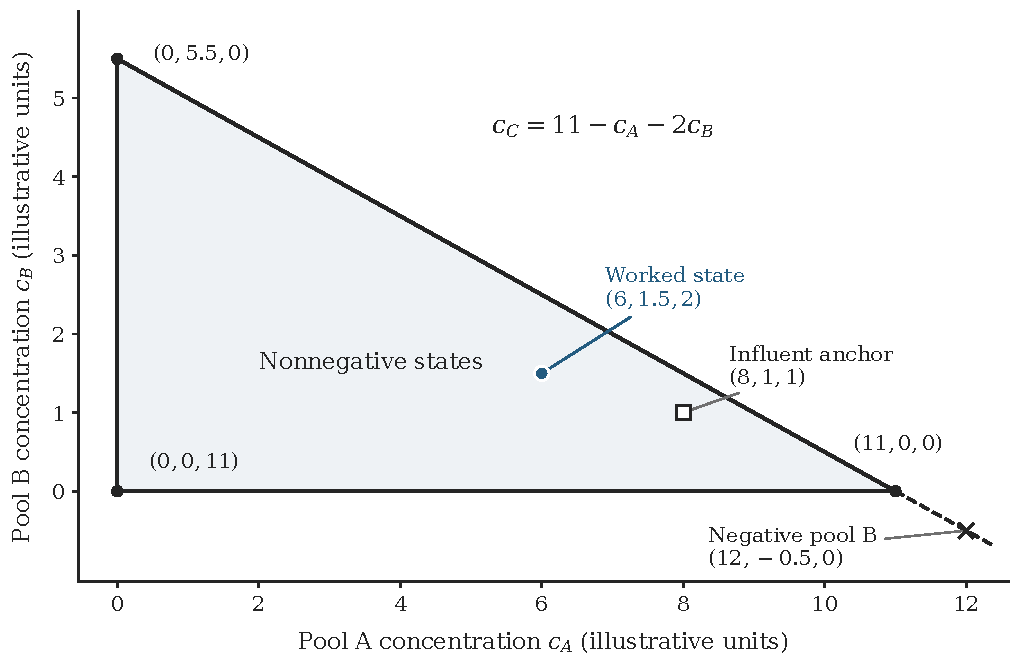
\includegraphics[width=0.93\textwidth]{ch3_concept_feasible_triangle.pdf}
\caption{Hypothetical non-negative states for the weighted inventory $c_A+2c_B+c_C=11$. The shaded triangle includes its boundary. Full state labels retain the third component even though only two coordinates are plotted.}
\label{fig:reactor_feasible_triangle}
\end{figure}

The sloping edge has $c_C=0$. The two coordinate edges have $c_A=0$ or $c_B=0$. Inside the triangle, all three components are positive and can redistribute the same inventory in different proportions. The cross-marked point preserves the inventory but has negative pool $B$. The figure therefore shows how concentration bounds reduce the inventory plane to a particular feasible region without selecting a unique kinetic state.

A two-component hypothetical system with sum fixed by mass conservation $c_1+c_2=10$ illustrates the geometry. The equality permits states such as $(-1,11)$, $(4,6)$, and $(12,-2)$. Non-negativity retains only the line segment between $(0,10)$ and $(10,0)$. Clipping $(-1,11)$ to $(0,11)$ sets its negative coordinate to zero but changes the sum to 11. Enforcing the equality alone and enforcing non-negativity alone therefore solve different problems. Simultaneous enforcement requires the intersection.

The geometry also explains why a feasible prediction need not be kinetically correct. Several non-negative states can share all five invariant values. A state with the wrong distribution between ammonium and nitrate may satisfy the invariant equality. A state with an implausible biomass concentration may do the same. The feasible set establishes the declared material accounting and sign restrictions. It does not establish that the 28 process rates balance hydraulics and aeration at that state. This distinction is central to the constraint methods of \citet{KircherVotsmeier2025} and to the broader physical-consistency perspective of \citet{Valente2025}.

\section{Reported water quality quantities and hidden component errors}

Reported water quality quantities are calculated after a component state has been predicted. Each quantity is first a scalar weighted sum of the components. The coefficients in Table~\ref{tab:component_basis_composites} give
\[
\begin{aligned}
\mathrm{COD}={}&S_F+S_A+S_I+X_I+X_S+X_H+X_{PAO}\\
&+X_{PHA}+X_{AOB}+X_{NOB},\\[2pt]
\mathrm{TN}={}&S_{NH4}+S_{NO2}+S_{NO3}+0.01S_I+0.02X_I\\
&+0.07(X_H+X_{PAO}+X_{AOB}+X_{NOB}),\\[2pt]
\mathrm{TP}={}&S_{PO4}+0.01X_I+0.02(X_H+X_{PAO}+X_{AOB}+X_{NOB})\\
&+X_{PP}+X_{MeP}/4.87,\\[2pt]
\mathrm{TSS}={}&0.75(X_I+X_S)+0.90(X_H+X_{PAO}+X_{AOB}+X_{NOB})\\
&+3.23X_{PP}+0.60X_{PHA}+X_{MeP}+X_{MeOH}.
\end{aligned}
\]
For example, the factor 0.07 has units of g nitrogen per g biomass COD. Multiplying it by $X_H$ on the biomass COD concentration basis produces a nitrogen concentration. The factor 3.23 has units of g suspended solids per g stored phosphorus. The sum for each reported quantity therefore combines contributions already converted to the same output basis.

A hypothetical reporting state containing only $X_H=100$ g COD m$^{-3}$ and $X_{PP}=2$ g P m$^{-3}$ gives
\[
\begin{aligned}
\mathrm{COD}&=100, &\mathrm{TN}&=0.07(100)=7,\\
\mathrm{TP}&=0.02(100)+2=4,
&\mathrm{TSS}&=0.90(100)+3.23(2)=96.46.
\end{aligned}
\]
Each numerical output uses its own reported constituent unit. This sparse example teaches the composition calculation and is not asserted to be a reactor steady state. The matrix map records these same four sums by placing the COD coefficients in its first row, the TN coefficients in its second row, and the remaining two coefficient groups in their corresponding rows. With the coefficients in Table~\ref{tab:component_basis_composites},
\begin{equation}
y=I_{comp}c,\qquad
y=(\mathrm{COD},\mathrm{TN},\mathrm{TP},\mathrm{TSS})^\top,\qquad
I_{comp}\in\mathbb{R}^{4\times20}.
\label{eq:component_composite_map}
\end{equation}
The four rows convert the component vector to g COD m$^{-3}$, g N m$^{-3}$, g P m$^{-3}$, and g TSS m$^{-3}$, respectively. All coefficients are non-negative. A non-negative component state therefore gives non-negative reported quantities.

The nitrogen map excludes dissolved dinitrogen. This reporting convention makes TN different from an inventory used for mass conservation that includes nitrogen gas. In a hypothetical redistribution of 3 g N m$^{-3}$ from nitrate to dissolved dinitrogen, the reported TN decreases by 3 g N m$^{-3}$ while the complete nitrogen inventory can remain unchanged. Conversely, a phosphorus inventory that includes every modeled phosphorus pool can coincide with a reporting row. The relationship between a reported total and an invariant must be checked from their coefficients rather than inferred from the word ``total.''

The same coefficient table explains constituent conversion. A hypothetical $X_H$ concentration of 100 g COD m$^{-3}$ contributes 100 g COD m$^{-3}$ to COD, 7 g N m$^{-3}$ to TN, 2 g P m$^{-3}$ to TP, and 90 g TSS m$^{-3}$ to TSS under the adopted map. A hypothetical $X_{PP}$ concentration of 2 g P m$^{-3}$ contributes 2 g P m$^{-3}$ to TP and 6.46 g TSS m$^{-3}$ to TSS. These examples illustrate fixed accounting factors rather than evidence about a treatment outcome.

Aggregation can hide prediction errors. Equal and opposite errors in ammonium and nitrate cancel in reported TN because both have unit nitrogen weights. A negative ammonium value can even be hidden by a sufficiently large nitrate prediction. Likewise, different biomass and substrate errors can compensate in COD while producing distinct errors in TSS because their solids factors differ. Four accurate reported quantities therefore cannot establish an accurate or physically admissible 20-component state.

The reporting map and the invariant operator serve different purposes. The map provides engineering summaries. The invariant operator tests reaction-compatible material accounting at the declared boundary. Neither can recover all of the component information lost by aggregation. Component prediction, composite interpretation, mass conservation, and non-negativity therefore remain separate objects of assessment.


\section{Mixing and spatial transport as model boundaries}

The preceding reactor balance assumes a single mixed concentration for each component in a reactor. This assumption removes spatial coordinates from that reactor state. It is a modeling decision rather than a claim that every treatment unit is uniform. Biofilms, trickling filters, and aerated vessels with incomplete mixing can have concentration gradients and transport limitations \citep{Wik2003,Zhang1994,SadinoRiquelme2020}. These effects provide useful context for interpreting the scope of a mixed-reactor surrogate.

A small spatial control volume illustrates the additional accounting. For one component, let $V$ be its fixed volume and $\bar c$ its average concentration. Let $F_{\rm adv,in}$ and $F_{\rm adv,out}$ be advective mass flow rates. Let $F_{\rm diff,in}$ and $F_{\rm diff,out}$ be diffusive mass flow rates. The finite-volume balance is
\begin{equation}
V\frac{\mathrm d\bar c}{\mathrm dt}
=F_{\rm adv,in}-F_{\rm adv,out}
+F_{\rm diff,in}-F_{\rm diff,out}+Vr.
\label{eq:teaching_spatial_control_volume}
\end{equation}
The symbol $r$ is the net reaction production rate per unit volume. It can be negative when the component is consumed. Every term on the right has units of component mass per time. For a hypothetical volume of 2 m$^3$, advective inflow and outflow of 5 and 3 g d$^{-1}$, diffusive inflow and outflow of 2 and 0 g d$^{-1}$, and total reaction consumption of 3 g d$^{-1}$, the accumulation is $5-3+2-0-3=1$ g d$^{-1}$. Dividing by the volume gives $\mathrm d\bar c/\mathrm dt=0.5$ g m$^{-3}$ d$^{-1}$. This calculation shows why the reaction term alone cannot determine a local concentration change.

In a one-dimensional domain with coordinate $z$, the advective flux is $v c$ and the diffusive flux is $-D_z\partial c/\partial z$. Here $v$ is the velocity and $D_z$ is a dispersion or diffusion coefficient. Dividing the balance of a slice by its volume and taking the limit as its thickness decreases gives
\begin{equation}
\frac{\partial c_j}{\partial t}
=-\frac{\partial(v c_j)}{\partial z}
+\frac{\partial}{\partial z}
\left(D_z\frac{\partial c_j}{\partial z}\right)
+\sum_{p=1}^{n_p}\nu_{pj}\rho_p+s_j.
\label{eq:teaching_spatial_balance}
\end{equation}
The term $s_j$ represents a specified external source per unit volume. The first two terms express spatial transport. The summation is the same component-by-component reaction accounting used in the mixed reactor. Boundary conditions specify how material enters and leaves the spatial domain. An invariant weighted sum cancels compatible reaction terms, but the transport and external-source terms still remain in its balance.

This spatial formulation explains how the theoretical ideas can extend to other treatment representations. It is not an additional spatial reactor in the present study. Chapter~\ref{ch:plant} uses mixed reactor stages and a layered clarifier. The stages represent sequential treatment conditions, while the clarifier layers represent solids transport and inventory. Their distinct boundaries must be respected when mass conservation is imposed.

\chapter{Learning the Reactor Response and Enforcing Physical Admissibility}
\label{ch:projection}

\section{Rationale}

Repeated activated sludge calculations are needed to compare influent conditions and operating settings. A surrogate can reduce the cost of these calculations by approximating responses learned from simulated cases. Its engineering value depends on what it predicts and how that prediction is checked. Organic substrate, nitrogen species, phosphorus, biomass, and solids all contribute to the treatment response and reactor material accounting \citep{Henze2006}. Predicting a few reported totals does not establish agreement with this complete state. Two effluents with the same TN can contain different amounts of ammonium and nitrate. A model that predicts the total correctly can therefore still misrepresent a treatment process of interest.

The first gap concerns comparative evidence for the complete activated sludge response. The soft sensor of \citet{Ching2022} estimates oxygen demand from available measurements, while \citet{Wang2025} compare methods for effluent TN prediction. The structured reactor study of \citet{Selerio2026} retains the complete effluent component state. These contributions support useful but different prediction tasks. Their findings do not by themselves establish which learning method best approximates the same complete state under a shared assessment. A meaningful comparison requires common influent and operating inputs, component targets, assessment cases, and error scales. Otherwise, differences in the prediction task can be mistaken for differences between learners.

Data availability is an important part of this gap. Generating training cases requires mechanistic reactor calculations, so the available simulation budget affects the practical choice of a surrogate. A flexible learner may perform well with many cases without being the best choice when only a small design is available. The learning-curve review of \citet{VieringLoog2023} explains why performance should be followed across data budgets. The tabular comparisons of \citet{Borisov2024} and \citet{ShwartzZiv2022} also support comparing several learning families rather than assuming that one family is consistently preferable. For activated sludge analysis, this comparison must retain the substrate, nutrient, biomass, and solids responses that the engineer intends to use.

Prediction beyond the sampled influent and operating ranges poses a separate question. A held-out case within those ranges tests a different use from an unfamiliar loading or operating condition. The study therefore examines learning-domain and exterior inputs separately. This distinction is important when a surrogate is used to explore alternatives rather than reproduce familiar cases. Neither a favorable learning-domain error nor a physically admissible exterior prediction establishes accurate treatment prediction beyond the sampled range \citep{KircherVotsmeier2025,Selerio2026}.

The second gap concerns simultaneous physical enforcement and its effect on the same reactor predictions. Ordinary regression approximates the statistical response without necessarily preserving the inventories or concentration bounds of a new influent. Physical guidance during fitting and explicit constraints on the returned state serve different purposes \citep{Kashinath2021,Hansen2024}. A balance check alone can accept a state with a negative component. Replacing that negative concentration with zero can then disturb the balance. Both requirements must therefore be checked on each returned state. The projection of \citet{KircherVotsmeier2025} provides a method for enforcing mass conservation and non-negativity together. The unresolved application question is how this common adjustment behaves across activated sludge learners, component scales, and input conditions.

Physical compliance is only one part of that assessment. Projection changes the component vector and can redistribute error among its entries. Those changes also alter COD, TN, TP, and TSS, which are reported treatment quantities rather than interchangeable measures of reactor conservation. The species-weighted correction of \citet{SturmSilva2024} shows why the scale assigned to an adjustment matters. An improvement in nutrient prediction can accompany a deterioration in another quantity. A single aggregate error or a count of feasible states cannot describe this tradeoff. Component errors, reported treatment errors, and physical checks are therefore needed together.

The adjustment also has a computational cost. A surrogate intended for repeated operating calculations must be assessed as the complete prediction procedure, including projection. Large changes from a raw state can reveal disagreement with the imposed physical relations, but small changes do not establish accurate reaction behavior. Paired raw and projected predictions allow error, physical compliance, displacement, and prediction cost to be examined without changing the fitted learner. This separation follows the need to assess approximation quality and computational usefulness together in surrogate applications \citep{BhosekarIerapetritou2018}.

The study addresses the first and second research questions in Section~\ref{sec:research_questions}. It compares complete reactor predictions across learning methods, simulation budgets, and input-domain conditions. It then assesses the effect of a common projection on those same predictions. The contribution is an activated sludge benchmark that separates learner performance from physical enforcement and identifies their joint consequences for treatment analysis. It does not introduce a new projection method or presume that projection improves every error measure. Its practical purpose is to support a choice of learner and adjustment procedure for specified data availability, treatment quantities, and operating ranges.

\section{Theory}

\subsection{Reactor inputs and raw predictions}

For sample $i$, the two operating values are entered first. They are followed by the twenty influent concentrations in the established component order. Written as a list, the input begins with $(\mathrm{HRT}_i,u_{\mathrm{air},i},S_{O,in,i},S_{F,in,i})$ and ends with the remaining influent coordinates through $X_{MeOH,in,i}$. The component list and its units are fixed before any learner is fitted. Transposing the two input blocks into rows permits their horizontal concatenation. The final transpose restores the column convention. The complete input for sample $i$ is
\begin{equation}
\equationname{Reactor surrogate inputs from operation and influent concentrations}
x_i=(u_i^\top,c_{in,i}^\top)^\top\in\mathbb{R}^{22},\qquad
u_i=(\mathrm{HRT}_i,u_{\mathrm{air},i})^\top.
\label{eq:surrogate_input_vector}
\end{equation}
A fitted surrogate is a function that takes these twenty-two numbers and returns twenty component values. The subscript $m$ identifies which fitted method is used. For component $j$, its prediction can be written as $c_{raw,ij}^{(m)}=f_{m,j}(x_{i1},\ldots,x_{i22})$. The superscript $(m)$ identifies the model and is not an exponent. Collecting its twenty scalar output functions, a fitted surrogate $f_m$ produces the raw component prediction
\begin{equation}
\equationname{Raw component-state prediction from a fitted surrogate}
c_{raw,i}^{(m)}=f_m(x_i)\in\mathbb{R}^{20}.
\label{eq:surrogate_raw_state}
\end{equation}
The raw prediction is assessed in its returned physical units. A post prediction projection then produces a second prediction for the same sample. Pairing the two states permits the effect of physical enforcement to be assessed separately from the choice of learner, data partition, and preprocessing \citep{SturmSilva2024,KircherVotsmeier2025}.

\subsection{Statistical response models}

\subsubsection{Boosting and randomized tree ensembles}

XGBoost builds an additive sequence of regression trees. A regression tree applies a sequence of input comparisons and assigns the value associated with the reached terminal region. For one output, an additive tree model has the scalar form
\[
f_j(x)=b_j+\beta_1h_{1j}(x)+\beta_2h_{2j}(x)+\cdots+\beta_Th_{Tj}(x).
\]
Here $h_{tj}$ is the response from tree $t$, $\beta_t$ determines its contribution, and $b_j$ is a baseline. The summation notation $b_j+\sum_{t=1}^T\beta_th_{tj}(x)$ records the same additions. A hypothetical baseline of 10 and two tree contributions of $-2$ and 1 produce 9. Each new tree addresses the error left by the current ensemble while regularization discourages an unnecessarily complex fit. Its split structure represents changes in response across input regions, and repeated additions permit interactions and nonlinear response shapes. The computational design and regularized objective of \citet{ChenGuestrin2016} motivate its inclusion as a flexible tabular baseline.

LightGBM also uses gradient-boosted trees, but grows trees through leaf-wise expansion. This strategy can allocate more detail to regions where an additional split offers a larger loss reduction. The efficiency-oriented design of \citet{Ke2017} makes the method relevant when each candidate fit must be repeated over several validation partitions. Its learning rate, leaf count, and minimum leaf support jointly control how closely it follows the training response.

CatBoost uses symmetric boosted trees and a Bayesian bootstrap in the specified regression setting. The work of \citet{Prokhorenkova2018} addresses bias associated with categorical-feature handling and boosting. The reactor benchmark evaluates this learner on continuous inputs. Each level of a symmetric tree uses the same splitting condition across nodes at that level. This structural restriction gives a different approximation class from the leaf-wise trees of LightGBM.

Adaptive boosting (AdaBoost) regression combines shallow trees through adaptive emphasis on observations that are difficult to predict. The base trees have depth three. The estimator count, learning rate, and loss choice control how strongly the ensemble responds to poorly fitted examples. \citet{Drucker1997} develops the regression extension of boosting that supports this comparator. These four boosting methods fit one regressor for each effluent component. All 20 regressors within a method use one shared selected hyperparameter vector.

Random Forest averages randomized regression trees. For component $j$, the average of $T$ tree responses is $f_j(x)=[h_{1j}(x)+\cdots+h_{Tj}(x)]/T$. Hypothetical tree values of 2, 3, and 4 give a mean of 3. Variation in sampled observations and candidate features reduces dependence among trees, so the average is less sensitive to a particular tree fit \citep{Breiman2001}. Extra Trees adds randomization of split thresholds \citep{Geurts2006}. Both methods fit the 20 outputs jointly in native multiresponse ensembles. Joint output handling lets the same tree partition support several component predictions. The projection subsequently enforces their stoichiometric relationships.

Tree averaging can preserve non-negativity when all leaf responses are non-negative. Mass conservation also requires the balance target of the new influent. For a hypothetical two-component system, two training responses with totals of 10 and 20 have an equally weighted average with total 15. If a new influent requires total 12, the average is positive but inconsistent with mass conservation for that sample. This distinction is caused by the sample-specific target $b_i$, rather than by whether the predictor averages positive observations.

\subsubsection{Kernel, neighborhood, and latent-variable regression}

Support vector regression (SVR) fits a function with an error-insensitive region around each training response. For scalar error $e$ and positive insensitive width $\epsilon$, its error contribution is zero when $|e|\leq\epsilon$ and $|e|-\epsilon$ otherwise. This can be recorded as $\max(0,|e|-\epsilon)$. With a hypothetical width of 0.2, an error of 0.1 contributes zero and an error of $-0.5$ contributes 0.3. Predictions within that region incur no corresponding error penalty. A linear kernel gives a globally linear input mapping. A radial kernel allows a nonlinear mapping through similarity to training inputs. Its similarity has the form
\[
K(z,z')=\exp\!\left[-\gamma\sum_{\ell=1}^{22}(z_\ell-z'_\ell)^2\right].
\]
Here $z$ and $z'$ contain the standardized input coordinates used by this learner. The positive coefficient $\gamma$ controls how quickly similarity decreases with squared distance. Identical inputs give similarity one. Greater distance gives a smaller value. The penalty parameter balances fit and regularity, while the insensitive width sets the tolerated response discrepancy. \citet{SmolaScholkopf2004} explain these mechanisms and the importance of their parameterization. The benchmark fits one regressor per component with one shared setting vector.

The $k$-nearest-neighbor ($k$-NN) predictor finds training observations close to a new input and combines their 20-component responses. For one component and a selected neighborhood $\mathcal N(x)$, weighted averaging means
\[
f_j(x)=\frac{\sum_{i\in\mathcal N(x)}w_i c_{out,ij}}{\sum_{i\in\mathcal N(x)}w_i}.
\]
The neighborhood size controls the degree of smoothing. Uniform weights give every selected neighbor equal influence, whereas distance weights give closer observations greater influence. Hypothetical neighbor values 2 and 6 give 4 under equal weights. Weights 3 and 1 instead give $[3(2)+1(6)]/(3+1)=3$. The local behavior analyzed by \citet{Mack1981} explains why input scaling and distance choice matter. An unscaled alkalinity coordinate spanning hundreds of numerical units could dominate a much smaller aeration coordinate even though both influence the reactor. Standardization avoids using native numerical range as an implicit measure of scientific importance.

Partial least squares (PLS) regression represents the inputs and joint response through latent directions chosen to capture their covariance. One latent score is a weighted input sum $t_h=w_{1h}z_1+\cdots+w_{22h}z_{22}$, where $z$ contains standardized inputs. An output is then a baseline plus a weighted sum of the retained scores. Substituting each score's input sum shows why ordinary partial least squares remains a linear input mapping. It can summarize strongly related input variables with a relatively small number of latent components. These weighted statistical combinations differ from the physical effluent components predicted by the model. The chemometric formulation described by \citet{Wold2001} provides an inspectable linear baseline. Its wastewater use is illustrated by \citet{Woo2009}, who employs a kernel extension for process-variable estimation, and by \citet{Yang2021}, who combines partial least squares with another predictor for adaptive effluent-quality prediction. The benchmark retains ordinary partial least squares with one to six latent components while predicting all 20 physical effluent components.

\subsubsection{Shared sparse coefficient models}

Multi-task Lasso fits one coefficient matrix for all component outputs. A predicted output is a baseline plus a sum of input-coefficient products. For two hypothetical inputs and two outputs, the coefficient rows can be $(3,4)$ and $(0,0)$. The first input contributes to both outputs and the second contributes to neither. The Euclidean length of the first row is $\sqrt{3^2+4^2}=5$, and the length of the second row is zero. Adding row lengths gives 5. This operation penalizes an input's complete coefficient group rather than adding the absolute value of every coefficient separately. If row $B_{j,\cdot}$ contains the coefficients of input $j$ across those outputs, the row-group penalty is
\begin{equation}
\equationname{Row-group penalty for multiresponse regression coefficients}
\|B\|_{2,1}=\sum_j\|B_{j,\cdot}\|_2.
\label{eq:multiresponse_row_penalty}
\end{equation}
This penalty can set an entire input row to zero. It therefore promotes a shared selection of inputs rather than 20 unrelated selections. The feature-sharing principle of \citet{Argyriou2008}, the multi-task Lasso algorithm of \citet{Liu2009}, and the grouped-variable framework of \citet{Yuan2006} provide the relevant foundations.

Multi-task Elastic Net combines the row-group penalty with a squared Frobenius penalty. The squared Frobenius norm is the sum of the squares of all matrix entries. For the hypothetical coefficient rows just given, it is $3^2+4^2+0^2+0^2=25$. With penalty strength $\lambda>0$ and mixing ratio $r\in(0,1)$, the combined penalty has the form
\[
\lambda r\sum_j\sqrt{\sum_{f=1}^{20}B_{jf}^2}
+\frac{\lambda(1-r)}2\sum_j\sum_{f=1}^{20}B_{jf}^2.
\]
For the two-output illustration only, taking $\lambda=0.2$ and $r=0.5$ gives $0.2(0.5)(5)+0.2(0.5)(25)/2=1.75$. The row-group part encourages selection and the squared part shrinks the retained coefficients. This extends the elastic-net principle of \citet{Zou2005} to a joint response structure, with multiresponse computation described by \citet{Simon2013}. Both methods use standardized inputs and targets. Their global coefficient matrices can be inspected to identify fitted associations. A nonzero row identifies an input that contributes to the fitted prediction.

These two predictors and partial least squares are grouped as structurally inspectable surrogates. The grouping identifies their globally available coefficient structures \citep{Rudin2019}. Physical projection enforces the influent-specific balances and non-negativity of their returned predictions.

\subsubsection{Neural predictors}

The multilayer perceptron (MLP) uses three fully connected hidden layers with 128, 64, and 32 units and one joint 20-output layer. One unit first forms a weighted sum, such as $b+w_1z_1+w_2z_2$, and then applies an activation. A rectified linear activation returns the larger of zero and that sum. For hypothetical values $b=0.2$, $w_1=0.5$, $w_2=-1$, $z_1=2$, and $z_2=0.3$, the sum is $0.2+0.5(2)-0.3=0.9$ and the activated value is 0.9. If the sum were $-0.9$, the activated value would be zero. Each hidden layer applies such operations to the values supplied by the preceding layer. Backpropagation updates the weights according to the prediction loss \citep{Rumelhart1986}. The approximation result of \citet{Hornik1989} motivates the expressive capacity of feedforward networks. The topology considerations discussed by \citet{Curteanu2011} motivate the stated architecture and training controls.

TabNet applies sequential attentive feature selection. At a decision step, a feature mask multiplies each input coordinate by its selected attention weight. If two hypothetical standardized inputs are $(2,1)$ and their mask weights are $(0.8,0.2)$, the masked inputs are $(1.6,0.2)$. A different step can use different weights and therefore examine a different input emphasis. The selected features then contribute to a joint output layer. \citet{ArikPfister2021} develop this approach for tabular learning. The attention masks show how the model weights its inputs during prediction. TabNet remains a neural comparator even though its internal masks can be inspected.

An epoch is one pass through the training data during neural fitting. Patience is the allowed number of consecutive epochs without the specified improvement before stopping. These fitting quantities describe the use of simulated reactor cases.

Both neural predictors start from random initialization and use only the simulated training partition available to that fit. The multilayer perceptron uses all available training rows and stops on training-loss convergence or at 250 epochs. Validation-based early stopping is disabled. Its training-loss patience is 15 epochs. TabNet's epoch count is selected in the inner search and ranges from 20 to 50. Its patience is zero, so a refit runs the selected epoch count without reserving an additional response-based stopping partition.

\subsection{Simultaneous physical requirements}

Now let the first hypothetical concentration be 11 and the second be $-1$. Their sum is $11+(-1)=10$, so the inventory equality is satisfied. The second component fails non-negativity. Replacing it by zero changes the sum to $11+0=11$. To return to the non-negative part of the line defined by mass conservation, both coordinates can be changed. The state with first concentration 10 and second concentration zero has sum ten and passes both checks.

The individual adjustments make the distinction explicit,
\[
\begin{aligned}
\text{raw state}&=(11,-1)^\top,\\
\text{clipped state}&=(11+0,-1+1)^\top=(11,0)^\top,\\
\text{jointly feasible state}&=(11-1,-1+1)^\top=(10,0)^\top.
\end{aligned}
\]
Clipping changes only the second coordinate. The joint projection also compensates in the first coordinate. An equality projection alone can retain a negative component, while clipping alone can violate an equality. The final assessment therefore checks both properties on the same returned state \citep{KircherVotsmeier2025,Haddad2010}.

Figure~\ref{fig:assessment_feasible_segment} places the three states on the line defined by mass conservation and its non-negative segment. Their positions show which requirement each state satisfies.

\begin{figure}[htbp]
\centering
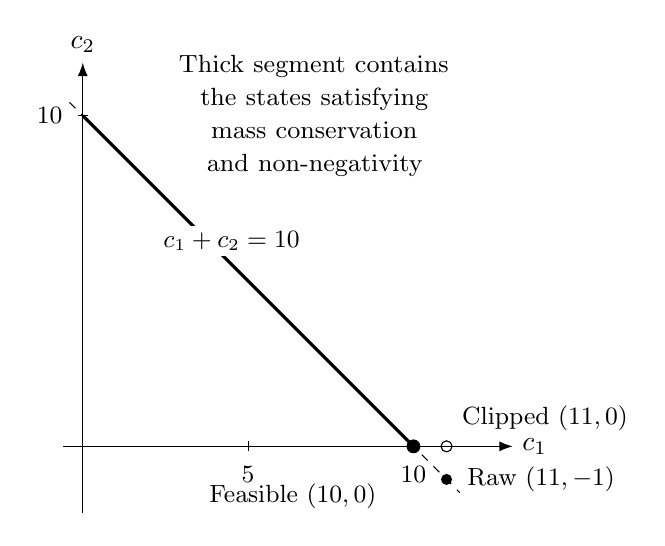
\begin{tikzpicture}[x=0.42cm,y=0.42cm,>=Latex]
\draw[->] (-0.6,0)--(13,0) node[right] {$c_1$};
\draw[->] (0,-2)--(0,11.6) node[above] {$c_2$};
\draw[dashed] (-0.4,10.4)--(11.4,-1.4);
\draw[very thick] (0,10)--(10,0);
\foreach \x in {5,10} {\draw (\x,0.15)--(\x,-0.15) node[below=2pt] {\small\x};}
\draw (0.15,10)--(-0.15,10) node[left=2pt] {\small 10};
\fill (11,-1) circle (2pt) node[right=4pt] {\small Raw $(11,-1)$};
\draw (11,0) circle (2pt) node[above right=3pt] {\small Clipped $(11,0)$};
\fill (10,0) circle (2.5pt);
\node[below left=14pt] at (10,0) {\small Feasible $(10,0)$};
\node[fill=white,inner sep=2pt] at (4.5,6.2) {\small $c_1+c_2=10$};
\node[align=center,text width=4cm] at (7,10) {\small Thick segment contains the states satisfying mass conservation and non-negativity};
\end{tikzpicture}
\caption{Hypothetical two-component geometry showing why clipping a negative concentration can violate a sum fixed by mass conservation.}
\label{fig:assessment_feasible_segment}
\end{figure}

The raw point is on the extended line defined by mass conservation but below the concentration boundary. The clipped point reaches a non-negative second coordinate while leaving that line. The jointly projected point lies at the end of the thick feasible segment. The geometry shows the two properties checked on each returned state.

Separate marginal summaries can also be misleading. If one prediction satisfies only mass conservation and another satisfies only non-negativity, neither is jointly feasible. For a hypothetical collection of two such states, each marginal compliance frequency is one half, while the joint compliance frequency is zero. The correct denominator is the number of states checked, and both conditions are tested within each state before counting joint compliance.

\subsection{The Kircher--Votsmeier projection for mass conservation and non-negativity}

\subsubsection{A positive provisional target and relative-error geometry}

\citet{KircherVotsmeier2025} develop a projection that combines mass conservation with non-negativity for mechanistic-kinetics surrogates. Its transfer to the reactor prediction problem uses the invariant operator $A$, the basis $Z$, and the feasible influent anchor. The projection depends on the completed component prediction rather than on predictor internals. It can therefore be applied to every comparator without changing its training objective or architecture. Its inputs are the full component vector, the corresponding non-negative influent, and the physical operators.

The first step compares each raw component with its positive floor. If a raw component is above the floor, its provisional value is the raw value. Otherwise, its provisional value is the floor. For component $j$, the operation is $c_{+,ij}^{(m)}=\max(c_{raw,ij}^{(m)},\varepsilon_{c,j})$. A hypothetical raw pair $(-0.2,3)$ becomes $(10^{-8},3)$ when both native-unit floors have value $10^{-8}$. The corresponding inverse values are $10^8$ and $1/3$. The floor gives a positive denominator for every provisional concentration. The subsequent projection enforces mass conservation.

A diagonal weighting matrix places each inverse concentration on its diagonal and zero elsewhere. For the hypothetical positive pair $(1,2)^\top$, its action on a discrepancy column $h$ is
\[
W=\begin{bmatrix}1&0\\0&1/2\end{bmatrix},\qquad
Wh=\begin{bmatrix}h_1\\h_2/2\end{bmatrix}.
\]
No component is mixed with another in this operation. Each component discrepancy is divided by its own provisional concentration, so both weighted coordinates are relative discrepancies. The first step forms a strictly positive provisional target,
\begin{equation}
\equationname{Positive provisional target and relative projection weights}
c_{+,i}^{(m)}=\max(c_{raw,i}^{(m)},\boldsymbol{\varepsilon}_c),\qquad
W_i^{(m)}=\operatorname{Diag}\bigl(\mathbf{1}\oslash c_{+,i}^{(m)}\bigr).
\label{eq:projection_positive_target}
\end{equation}
The maximum and division are componentwise. Each entry of $\boldsymbol{\varepsilon}_c$ is $10^{-8}$ in its component's native unit. The provisional target supplies both a reference state and finite positive weights. The subsequent mass conservation and non-negativity stages determine the final physical prediction.

For a component change $h_j$, the weighted discrepancy is $h_j/c_{+,ij}^{(m)}$. The geometry therefore penalizes relative movement. A hypothetical movement of 1 g m$^{-3}$ corresponds to a relative discrepancy of 0.01 at a component value of 100 g m$^{-3}$ and 10 at a component value of 0.1 g m$^{-3}$. Small coordinates receive strong protection. Large coordinates can absorb larger absolute changes at the same relative cost. Relative-error projection and variance-standardized accuracy therefore assess redistribution using different scales \citep{KircherVotsmeier2025,SturmSilva2024}.

\subsubsection{Selecting a candidate that satisfies mass conservation}

Changes consistent with mass conservation can first be written one component at a time. If $Z$ has fifteen change columns, coordinate $j$ of a change is $Z_{j1}q_1+\cdots+Z_{j,15}q_{15}$. Adding that change to $c_{in,ij}$ gives the candidate component. Since each column of $Z$ has zero invariant product, every such combination preserves the influent target.

A complete two-component hypothetical calculation shows how these coordinates are chosen. Both components use the same abstract concentration basis. Let the required sum be four and the feasible anchor be $(2,2)^\top$. The raw pair is $(1,2)^\top$, which sums to three. The provisional pair is unchanged because both values exceed the floor. A normalized invariant row and a normalized change column are
\[
A_{\rm ex}=\frac1{\sqrt2}\begin{bmatrix}1&1\end{bmatrix},\qquad
Z_{\rm ex}=\frac1{\sqrt2}\begin{bmatrix}1\\-1\end{bmatrix}.
\]
Their product is $(1-1)/2=0$. A scalar change amount $t$ gives the candidate $(2+t,2-t)^\top$. In the normalized basis its coordinate is $q=\sqrt2t$, because $Z_{\rm ex}q=(t,-t)^\top$. The sum remains four for every $t$. All states consistent with mass conservation for sample $i$ have the form
\begin{equation}
\equationname{Null-space parameterization of states satisfying mass conservation}
c=c_{in,i}+Zq,\qquad q\in\mathbb{R}^{15}.
\label{eq:projection_affine_parameterization}
\end{equation}
For the hypothetical pair, the provisional target change from the anchor is $(-1,0)^\top$. The difference between an allowed change and this target change is $(t+1,-t)^\top$. Applying the inverse provisional concentrations gives $(t+1,-t/2)^\top$. Its squared Euclidean norm is
\[
E(t)=(t+1)^2+\frac{t^2}{4}.
\]
At $t=0$, this value is one. Choosing a negative $t$ moves the first component toward its raw value while requiring an increase in the second to preserve the sum. A derivative describes the change in the objective for a small change in $t$. The derivative of $(t+1)^2$ is $2(t+1)$ and that of $t^2/4$ is $t/2$. Adding them gives the rate of change of the complete objective. The best compromise can be found by differentiating,
\[
\frac{dE}{dt}=2(t+1)+\frac t2=\frac52t+2.
\]
Setting the derivative to zero gives $t=-4/5$. The second derivative is $5/2>0$, so this point is the unique minimum. The resulting candidate is $(6/5,14/5)^\top=(1.2,2.8)^\top$. Its relative discrepancies from the provisional target are 0.2 and 0.4, giving squared objective $0.2^2+0.4^2=0.20$. A candidate $(1.5,2.5)^\top$ instead gives $0.5^2+0.25^2=0.3125$. The weighting favors the first candidate because the smaller provisional component receives stronger protection against absolute movement.

Figure~\ref{fig:relative_projection_geometry} shows this calculation as a geometric comparison. Curves around the raw pair connect states with the same projection objective. The line defined by mass conservation restricts the candidate to states whose two components sum to four.

\begin{figure}[htbp]
\centering
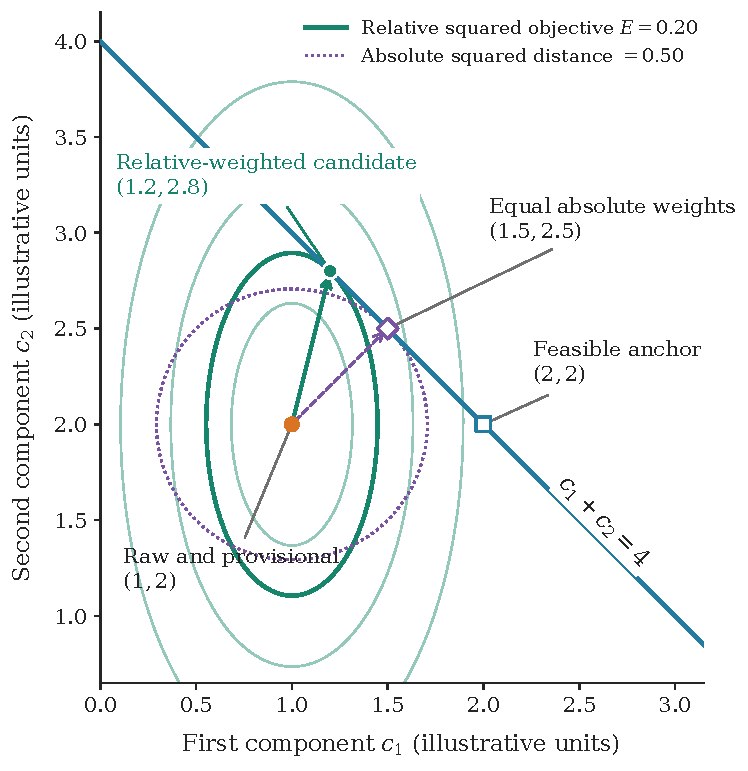
\includegraphics[width=0.79\textwidth]{ch4_concept_weighted_projection.pdf}
\caption{Hypothetical projection for mass conservation with relative and equal absolute weights. The highlighted ellipse first touches the line defined by mass conservation at the relative-weighted candidate. The dotted circle touches it at the equal-absolute-weight candidate.}
\label{fig:relative_projection_geometry}
\end{figure}

The relative-weighted ellipse is taller than it is wide because movement in the second component is divided by two. A larger absolute change in that component can therefore have the same weighted cost as a smaller change in the first. The circular geometry assigns equal cost to equal absolute changes. Both chosen points satisfy the sum fixed by mass conservation, but the distance definition determines where each geometry touches that line. The feasible anchor locates the reference from which changes satisfying mass conservation are constructed and need not be the nearest candidate.

For the full problem, let $d_j=c_{+,ij}^{(m)}-c_{in,ij}$ denote the provisional change and let $w_j=1/c_{+,ij}^{(m)}$. The scalar objective adds all twenty squared relative discrepancies,
\[
E(q)=\sum_{j=1}^{20}
w_j^2\left(\sum_{k=1}^{15}Z_{jk}q_k-d_j\right)^2.
\]
The inner sum builds one component of the change satisfying mass conservation. Subtracting $d_j$ gives its discrepancy from the target change. Multiplication by $w_j^2$ scales its square. The outer sum combines these component contributions. The notation $\operatorname{argmin}$ identifies the coordinate vector at which this objective is smallest, rather than the value of the objective itself. The projection selects the change satisfying mass conservation closest to the provisional target change in the relative-error geometry,
\begin{equation}
\equationname{Weighted least-squares problem for projection coordinates}
q_i^{*,(m)}=\underset{q\in\mathbb{R}^{15}}{\operatorname{argmin}}
\left\|W_i^{(m)}\bigl[Zq-(c_{+,i}^{(m)}-c_{in,i})\bigr]\right\|_2^2.
\label{eq:projection_weighted_least_squares}
\end{equation}
The squared objective is a quadratic function of $q$. To minimize it, differentiate with respect to each coordinate $q_\ell$. A partial derivative, written with $\partial$, varies this one coordinate while holding the others fixed. Differentiating the square and then its inner sum gives
\[
\frac{\partial E}{\partial q_\ell}
=2\sum_{j=1}^{20}w_j^2 Z_{j\ell}
\left(\sum_{k=1}^{15}Z_{jk}q_k-d_j\right).
\]
Set this derivative to zero, divide by two, and move the target-change contribution to the right-hand side. For every $\ell$, the resulting equation is
\[
\sum_{k=1}^{15}\left(\sum_{j=1}^{20}w_j^2Z_{j\ell}Z_{jk}\right)q_k
=\sum_{j=1}^{20}w_j^2Z_{j\ell}d_j.
\]
The coefficient of $q_k$ is a weighted dot product of columns $\ell$ and $k$ of $Z$. Because $W_i^{(m)}$ is diagonal, its square places $w_j^2$ on the diagonal. Collecting these fifteen equations gives a $15\times15$ coefficient matrix and a fifteen-coordinate right-hand side. Differentiation gives
\begin{equation}
\equationname{Normal equations for weighted projection coordinates}
Z^\top(W_i^{(m)})^2Zq_i^{*,(m)}
=Z^\top(W_i^{(m)})^2(c_{+,i}^{(m)}-c_{in,i}).
\label{eq:projection_normal_conditions}
\end{equation}
For the hypothetical pair, the compact coefficient calculation gives $Z_{\rm ex}^\top W^2Z_{\rm ex}=(1+1/4)/2=5/8$. Its right-hand side is $-1/\sqrt2$. Dividing gives $q^*=-8/(5\sqrt2)=-4\sqrt2/5$, which equals $\sqrt2t$ for the scalar minimum already obtained. The scalar and matrix calculations therefore return the same candidate. For any nonzero vector $v$, the full problem's associated quadratic form equals $\|W_i^{(m)}Zv\|_2^2>0$. If $Zv$ were zero, multiplying by $Z^\top$ would give $v=Z^\top Zv=0$, contradicting the choice of $v$. Positive diagonal weights cannot turn a nonzero column into zero. The squared norm is consequently strictly positive. A positive-definite matrix has a strictly positive such product in every nonzero direction. The matrix is therefore positive definite and the minimizer is unique.

The selected coordinates build the component change through the fifteen sums $\sum_kZ_{jk}q_k^*$. Adding each sum to its matching influent coordinate constructs the state. In the hypothetical pair, this operation is $(2,2)^\top+(-0.8,0.8)^\top=(1.2,2.8)^\top$. Both entries are non-negative and their invariant value is $(1.2+2.8)/\sqrt2=4/\sqrt2$, equal to the anchor value. This example needs no projection interpolation for non-negativity. The candidate satisfying mass conservation is
\begin{equation}
\equationname{Component candidate satisfying mass conservation}
c_{cand,i}^{(m)}=c_{in,i}+Zq_i^{*,(m)}.
\label{eq:projection_conservative_candidate}
\end{equation}
Since $AZ=0$, it satisfies $Ac_{cand,i}^{(m)}=Ac_{in,i}=b_i$ in exact arithmetic. If the provisional target is already consistent with mass conservation, its change lies in $\operatorname{null}(A)$. The least-squares residual can then be zero and the candidate reproduces that target to numerical tolerance.

Equation~\eqref{eq:projection_normal_conditions} provides the derivation rather than the preferred numerical solution. The weighted design $W_i^{(m)}Z$ is solved through an orthogonal--triangular factorization. Singular-value decomposition with relative cutoff $10^{-12}$ is the fallback. No explicit inverse of the normal-equation matrix is formed. Near-zero provisional targets can produce very unequal weights, so solving the original weighted system avoids the extra conditioning penalty associated with forming a normal-equation inverse \citep{BuzziFerraris2013}.

\subsubsection{The largest feasible interpolation toward the candidate}

The candidate is also checked for non-negativity. A different hypothetical three-component example isolates the boundary problem. Its quantity used for mass conservation is the unweighted sum, with feasible influent $(8,1,1)^\top$ and candidate satisfying mass conservation $(4,-0.5,6.5)^\top$. Both sums are ten. Subtracting the influent from the candidate gives the direction $(-4,-1.5,5.5)^\top$. A fraction $\alpha$ of that direction gives individual concentrations
\[
c_1(\alpha)=8-4\alpha,\qquad
c_2(\alpha)=1-1.5\alpha,\qquad
c_3(\alpha)=1+5.5\alpha.
\]
The first component requires $8-4\alpha\geq0$, so $\alpha\leq2$. The second requires $1-1.5\alpha\geq0$, so $\alpha\leq2/3$. The third increases and gives no upper bound for $\alpha\geq0$. Restricting $\alpha$ to $[0,1]$ makes $2/3$ the first boundary point. Define
\begin{equation}
\equationname{Candidate direction from the feasible influent anchor}
\delta_i^{(m)}=c_{cand,i}^{(m)}-c_{in,i}=Zq_i^{*,(m)}.
\label{eq:projection_candidate_direction}
\end{equation}
The segment $c_{in,i}+\alpha\delta_i^{(m)}$, with $0\leq\alpha\leq1$, satisfies mass conservation because $A\delta_i^{(m)}=0$. For a general decreasing coordinate, start with $c_{in,ij}+\alpha\delta_{ij}^{(m)}\geq0$. Moving the negative change to the other side gives $c_{in,ij}\geq\alpha(-\delta_{ij}^{(m)})$. The factor $-\delta_{ij}^{(m)}$ is positive, so dividing by it preserves the inequality direction. For every decreasing coordinate, non-negativity requires
\begin{equation}
\equationname{Interpolation bound for a decreasing concentration}
\alpha\leq\frac{c_{in,ij}}{-\delta_{ij}^{(m)}}
\qquad\text{when }\delta_{ij}^{(m)}<0.
\label{eq:projection_coordinate_bound}
\end{equation}
The minimum of these bounds is the first point at which the segment reaches the non-negative-orthant boundary.

If every candidate coordinate is non-negative, the entire direction is allowed and $\alpha=1$. If at least one candidate coordinate is negative, the smallest decreasing-coordinate ratio supplies a bound below one. Taking that bound reaches the concentration boundary. Multiplication by $1-\eta$ retreats slightly from the boundary to limit a sign change caused by rounding. With numerical safety margin $\eta=10^{-12}$, the accepted interpolation factor and final state are
\begin{equation}
\equationname{Interpolation factor and final state satisfying non-negativity}
\begin{split}
\alpha_i^{(m)}&=
\begin{cases}
1, & c_{cand,i}^{(m)}\geq0,\\
(1-\eta)\displaystyle\min_{j\,\mid\,\delta_{ij}^{(m)}<0}
\frac{c_{in,ij}}{-\delta_{ij}^{(m)}}, & \text{otherwise},
\end{cases}\\
\tilde c_i^{(m)}&=c_{in,i}+\alpha_i^{(m)}\delta_i^{(m)}.
\end{split}
\label{eq:projection_positivity_backtracking}
\end{equation}
If the candidate is negative somewhere, at least one bound lies below one. Non-negativity of the influent makes every bound non-negative. The factor is restricted to $[0,1]$ against roundoff. Decreasing coordinates satisfy $\tilde c_{ij}^{(m)}\geq\eta c_{in,ij}\geq0$, and increasing coordinates remain non-negative. For invariant row $h$, the final weighted component sum is $\sum_jA_{hj}c_{in,ij}+\alpha\sum_jA_{hj}\delta_{ij}^{(m)}$. The second sum is zero and the first is $b_{ih}$. Mass conservation follows from
\begin{equation}
\equationname{Mass conservation identity for the final projected state}
A\tilde c_i^{(m)}=Ac_{in,i}+\alpha_i^{(m)}AZq_i^{*,(m)}=b_i.
\label{eq:projection_final_conservation}
\end{equation}
The unrestricted boundary factor is the largest feasible interpolation factor. The safety margin makes the returned factor slightly smaller when projection is necessary.

A hypothetical three-component system with sum fixed by mass conservation 10 illustrates this safeguard. Let the feasible influent be $(8,1,1)^\top$ and a candidate satisfying mass conservation be $(4,-0.5,6.5)^\top$. The direction is $(-4,-1.5,5.5)^\top$. Its decreasing-coordinate bounds are 2 and $2/3$, so the largest feasible factor is $2/3$. Ignoring the numerical safety margin only for this illustration gives $(16/3,0,14/3)^\top$. The sum remains 10 and every component is non-negative. The first coordinate changes even though the second coordinate determines the boundary. One scalar shortens the complete direction satisfying mass conservation.

If an influent coordinate is zero and the candidate direction decreases that coordinate, its bound is zero. The final state then returns to the influent anchor. This returns a feasible state. Likewise, a component that is absent from the invariant rows can still move during interpolation because the complete direction is shortened. Recording the factor and activation frequency is therefore necessary for interpreting the projection.

\subsubsection{Numerical acceptance and returned predictions}

Numerical acceptance tests the returned state rather than assuming that the exact algebra eliminates rounding error. For row $h$, form the residual $r_h=\sum_jA_{hj}\tilde c_{ij}^{(m)}-b_{ih}$. Square its five values, add them, and take the square root to obtain the mass conservation norm. Separately compare each of the twenty concentrations with the negative of its own tolerance. A hypothetical concentration of $-5\times10^{-11}$ passes a $10^{-10}$ sign tolerance, whereas $-2\times10^{-10}$ fails it. These examples illustrate the numerical sign check. A returned projection is accepted only when
\begin{equation}
\equationname{Numerical mass conservation and non-negativity acceptance checks}
\|A\tilde c_i^{(m)}-b_i\|_2\leq\tau_{mc},\qquad
\tilde c_{ij}^{(m)}\geq-\tau_{nn,j}\quad\text{for every }j,
\label{eq:projection_numerical_acceptance}
\end{equation}
with $\tau_{mc}=10^{-10}$ in the fixed invariant-coordinate convention and $\tau_{nn,j}=10^{-10}$ in the native unit of component $j$. These checks distinguish the exact mathematical construction from its finite-precision realization. A finite raw vector is required.

The final state satisfies the declared invariants and sign restrictions. The least-squares stage minimizes weighted distance over the affine space, and the interpolation stage selects a feasible point on the influent-to-candidate line segment. The prediction error uses training standard deviations, while the projection weights use the positive provisional concentrations. These definitions give the two calculations distinct objectives.

Figure~\ref{fig:projection_acceptance_flow} brings the projection steps and their checks into one prediction procedure. The non-negativity decision concerns the candidate satisfying mass conservation. The final numerical audit applies to the state returned by either branch.

\begin{figure}[htbp]
\centering
\begingroup
\linespread{1}\selectfont
\begin{tikzpicture}[
    >=Latex,
    block/.style={draw=plantblue!85!black,fill=white,rounded corners=2pt,
        text width=4.2cm,minimum height=1cm,align=center,font=\small},
    branch/.style={draw=plantblue!85!black,fill=white,rounded corners=2pt,
        text width=4.1cm,minimum height=1.3cm,align=center,font=\small},
    test/.style={diamond,draw=plantblue!85!black,fill=plantteal!9,aspect=2.5,
        text width=2.7cm,align=center,inner sep=2pt,font=\small},
    flow/.style={->,line width=.9pt,draw=plantblue!85!black},
    tag/.style={font=\small,fill=white,inner sep=2pt}]
\node[block,draw=plantorange!85!black,fill=plantorange!10] (raw) at (0,0) {Raw prediction\\Physical units};
\node[block,draw=plantblue!85!black,fill=plantblue!10] (positive) at (0,-1.65) {Positive target\\Relative weights};
\node[block,draw=plantpurple!85!black,fill=plantpurple!10] (candidate) at (0,-3.3) {Candidate satisfying mass conservation\\Weighted solve};
\node[test,draw=plantteal!85!black,fill=plantteal!10] (non-negative) at (0,-5.2) {Candidate\\non-negative?};
\node[branch,draw=plantteal!85!black,fill=plantteal!10] (full) at (-3.0,-7.3) {Retain full change\\$\alpha=1$};
\node[branch,draw=plantpurple!85!black,fill=plantpurple!10] (shorten) at (3.0,-7.3) {Shorten toward influent\\Boundary ratio};
\coordinate (join) at (0,-8.4);
\node[test,draw=plantteal!85!black,fill=plantteal!10] (audit) at (0,-9.9) {Final numerical\\checks passed?};
\node[branch,draw=plantteal!85!black,fill=plantteal!10] (return) at (-3.0,-12.1) {Checked state\\Reported quantities};
\node[branch,draw=plantorange!85!black,fill=plantorange!10] (failure) at (3.0,-12.1) {Projection failure\\No unchecked output};
\draw[flow] (raw)--(positive);
\draw[flow] (positive)--(candidate);
\draw[flow] (candidate)--(non-negative);
\draw[flow] (non-negative.west)-|(full.north) node[pos=.25,tag] {Yes};
\draw[flow] (non-negative.east)-|(shorten.north) node[pos=.25,tag] {No};
\draw[draw=plantblue!85!black,line width=.9pt] (full.south)|-(join);
\draw[draw=plantblue!85!black,line width=.9pt] (shorten.south)|-(join);
\draw[flow] (join)--(audit.north);
\draw[flow] (audit.west)-|(return.north) node[pos=.25,tag] {Yes};
\draw[flow] (audit.east)-|(failure.north) node[pos=.25,tag] {No};
\end{tikzpicture}
\endgroup

\caption{Post prediction mass conservation and non-negativity procedure. Positive-target construction, projection for mass conservation, and final-state acceptance have separate roles. The diagram shows the sequence used for each prediction.}
\label{fig:projection_acceptance_flow}
\end{figure}

The provisional positive target supplies a reference and weights for the mass conservation solve. A non-negative candidate can retain the full change satisfying mass conservation, while a candidate crossing a concentration boundary requires shortening toward the feasible influent. Both branches reach the same final checks. This arrangement applies the same numerical acceptance criteria to each returned state.

Each raw or projected composite is obtained by multiplying the relevant component values by the coefficients already defined in Table~\ref{tab:component_basis_composites} and adding them. The coefficients do not change between the two prediction types. A paired comparison therefore changes only the component state supplied to the four scalar sums. Raw and projected composites are calculated with the same map,
\begin{equation}
\equationname{Raw and projected water-quality composites}
y_{raw,i}^{(m)}=I_{comp}c_{raw,i}^{(m)},\qquad
\tilde y_i^{(m)}=I_{comp}\tilde c_i^{(m)}.
\label{eq:projection_paired_composites}
\end{equation}
Feasibility is checked on the complete component state before this aggregation.

\section{Methodology}

\subsection{Constructing a mechanistic learning domain}

The single-reactor dataset is designed to contain 10,000 accepted steady states. Each candidate varies all 22 input coordinates. A randomized, scrambled, strength-one Latin hypercube places one sample in each stratum of every marginal input distribution. A stratum is one interval in a partition of an input range. A marginal distribution describes one coordinate, such as influent ammonium, considered separately from the other inputs. The construction uses seed 42 and no subsequent design optimization. Linear scaling maps the unit-hypercube samples to the bounds in Table~\ref{tab:reactor_sampling_domain}. Latin hypercube sampling distributes coverage across marginal ranges without requiring a full Cartesian grid \citep{McKay1979}.

\begin{table}[htbp]
\centering\small
\caption{Design bounds for the standalone reactor learning domain. The intervals define the sampled input ranges.}\label{tab:reactor_sampling_domain}
\begin{tabular}{lp{5.7cm}ll}
\toprule
Input & Meaning & Interval & Unit\\
\midrule
HRT & Hydraulic operating input & $[6,36]$ & h\\
$u_{\mathrm{air}}$ & Dimensionless aeration input & $[0.5,2.5]$ & 1\\
$S_O$ & Influent dissolved oxygen & $[0,0.5]$ & g O$_2$ m$^{-3}$\\
$S_F$ & Influent fermentable substrate & $[20,180]$ & g COD m$^{-3}$\\
$S_A$ & Influent acetate & $[5,80]$ & g COD m$^{-3}$\\
$S_{NH4}$ & Influent ammonium nitrogen & $[12,55]$ & g N m$^{-3}$\\
$S_{NO2}$ & Influent nitrite nitrogen & $[0,3]$ & g N m$^{-3}$\\
$S_{NO3}$ & Influent nitrate nitrogen & $[0,8]$ & g N m$^{-3}$\\
$S_{N2}$ & Influent dissolved dinitrogen & $[0,2]$ & g N m$^{-3}$\\
$S_{PO4}$ & Influent soluble phosphate & $[2,18]$ & g P m$^{-3}$\\
$S_I$ & Influent soluble inert organic matter & $[10,90]$ & g COD m$^{-3}$\\
$S_{ALK}$ & Influent alkalinity & $[80,260]$ & mol m$^{-3}$\\
$X_I$ & Influent particulate inert matter & $[20,120]$ & g COD m$^{-3}$\\
$X_S$ & Influent slowly biodegradable substrate & $[60,280]$ & g COD m$^{-3}$\\
$X_H$ & Influent heterotrophic biomass & $[15,100]$ & g COD m$^{-3}$\\
$X_{PAO}$ & Influent phosphate-accumulating biomass & $[5,60]$ & g COD m$^{-3}$\\
$X_{PP}$ & Influent stored polyphosphate & $[2,20]$ & g P m$^{-3}$\\
$X_{PHA}$ & Influent stored polyhydroxyalkanoates & $[1,30]$ & g COD m$^{-3}$\\
$X_{AOB}$ & Influent ammonia-oxidizing biomass & $[0.5,8]$ & g COD m$^{-3}$\\
$X_{NOB}$ & Influent nitrite-oxidizing biomass & $[0.5,8]$ & g COD m$^{-3}$\\
$X_{MeP}$ & Influent precipitated metal phosphate & $[0,12]$ & g TSS m$^{-3}$\\
$X_{MeOH}$ & Influent metal hydroxide & $[0,12]$ & g TSS m$^{-3}$\\
\bottomrule
\end{tabular}
\end{table}

The standalone domain varies the operating and influent inputs within the declared simulation bounds. Its alkalinity interval uses the stated native coordinate. The coupled plant uses its own operating and influent bounds.

For each candidate input, nonlinear least squares solves Equation~\eqref{eq:reactor_steady_balance} with numerical state bounds $[10^{-8},1500]$ in each component's native unit. The cost-change, step-size, and gradient convergence tolerances are $10^{-9}$. Each solve allows at most 1200 function evaluations. The generation procedure has an overall attempt cap of 25 times the target retained count. A state is retained only if the solver converges and the maximum absolute component-balance residual is no greater than $10^{-9}$ on the fixed native component-unit-per-day coordinates. The residual criterion uses the native component-unit-per-day coordinates.

Two physically informed starting states are tried before dynamic relaxation. The first blends the sampled influent with a preceding accepted effluent when one is available. It lowers readily consumed substrate coordinates, retains biomass pools, and estimates dissolved oxygen from dilution and transfer. The second applies stronger substrate depletion and biomass enrichment. Starting vectors are restricted to $[10^{-6},1500]$. If both steady solves fail, a stiff backward differentiation formula integrates the dynamic balance for 20 days and supplies a new initial state. The state bounds and starting-state restrictions apply to concentrations. The 28 kinetic process rates are evaluated without an artificial ceiling or clipping.

Solver acceptance, invariant residual, and minimum concentration are recorded separately. A converged bounded least-squares calculation can terminate without meeting the required balance residual. A positive state can also fail mass conservation. Retaining these separate diagnostics prevents one successful numerical check from standing in for all others. The surrogate inputs contain the sampled operating and influent coordinates. Initialization choices and solver history are not predictive features.

\subsection{Preprocessing and validation without response leakage}

A fold is one reserved group of cases in cross-validation. Successive fits change which group is withheld. Nested cross-validation separates an inner comparison used to select hyperparameters from an outer comparison used to assess the selected model. Here each case contains influent and operating inputs paired with the mechanistic effluent state.

The evaluation uses nested subsets at
\begin{equation}
\equationname{Observation counts for nested reactor assessment}
N\in\{500,1450,2400,3350,4300,5250,6200,7150,8100,9050,10000\}.
\label{eq:reactor_nested_sample_sizes}
\end{equation}
A seed-42 permutation determines the nested row order and persistent master fold identifiers before subsets are formed. Every smaller subset is contained in each larger subset. A row retains its outer-fold role at every scale. Five outer folds train on $0.8N$ observations and score the remaining $0.2N$. Thus a design size of 500 gives 400 training rows and 100 scored rows per outer iteration. A design size of 10,000 gives 8000 training rows and 2000 scored rows. The five iterations change which fold is withheld, so each row supplies a scored prediction from a fit that excludes it. The same rows and fold identifiers are used by every surrogate and both prediction types.

Hyperparameters are selected using four inner folds within the largest outer-training partition. The scored outer fold is absent from the search. Within an 8000-row outer-training pool, an inner iteration fits on 6000 rows and scores 2000 different rows from that pool. Those inner-validation rows are not the 2000 rows reserved for outer assessment. The inner score selects the setting, and the outer score assesses a model fitted with that selected setting. For each outer fold, its selected setting is retained over the smaller nested subsets. Learning curves therefore examine the response to sample size under a fixed fold-specific setting. The bias--variance discussion of \citet{Belkin2019} cautions against assuming that error must vary monotonically with model capacity or available data. The learning-curve review of \citet{VieringLoog2023} supports treating the complete curve as an object of assessment.

Every transformation is fitted within the applicable training partition. During inner selection, that partition is the inner-training split. During outer scoring, it is the outer-training subset at the current size. During extrapolation assessment, it is the full in-domain training pool. A training coordinate has one mean and one standard deviation for that fit. If its $M$ training values are $v_1,\ldots,v_M$, these quantities are calculated in three steps,
\[
\mu=\frac{v_1+\cdots+v_M}{M},\qquad
\sigma^2=\frac{(v_1-\mu)^2+\cdots+(v_M-\mu)^2}{M},\qquad
\sigma=\sqrt{\sigma^2}.
\]
The second quantity is the population variance. The population convention divides by the training count $M$. A z-score subtracts the mean and divides by the standard deviation, giving $z=(v-\mu)/\sigma$. Subtracting the mean centers the coordinate and division puts its numerical variation on a unit-standard-deviation scale. The transformation requires $\sigma>0$.

For hypothetical training values 2, 2, 6, and 6, the mean is 4. Their centered values are $-2$, $-2$, 2, and 2, so the variance is $(4+4+4+4)/4=4$ and the standard deviation is 2. A validation value of 6 therefore becomes $(6-4)/2=1$. The validation value is not added to the training values before calculating the mean or variance. If this coordinate is an output, a predicted z-score of 0.5 returns to physical units as $4+2(0.5)=5$.

The mean and population standard deviation of a training coordinate define its z-score transformation. Validation inputs are transformed with those training quantities, and target-scaled predictions are restored to physical units before projection or physical diagnostics. Every target has its own inverse transformation $\widehat c_j=\mu_j+\sigma_j\widehat z_j$. A single common inverse scale would be incorrect for components with different units or variability.

\begin{table}[htbp]
\centering
\caption{Output handling and preprocessing for the statistical comparators. Scaling uses only the training partition applicable to each fit.}
\label{tab:surrogate_preprocessing}
\small
\begin{tabular}{p{5.1cm}p{3.2cm}p{3.3cm}}
\toprule
Surrogates & Output handling & Scaling\\
\midrule
XGBoost, LightGBM, CatBoost & Separate component regressors & None\\
AdaBoost & Separate component regressors & Targets only\\
Random Forest & Joint tree response & None\\
Extra Trees & Joint tree response & Targets only\\
Support vector regression & Separate component regressors & Inputs and targets\\
$k$-nearest neighbors & Joint neighborhood response & Inputs and targets\\
Partial least squares, Multi-task Lasso, Multi-task Elastic Net & Joint coefficient structure & Inputs and targets\\
Multilayer perceptron, TabNet & Joint neural output & Inputs and targets\\
\bottomrule
\end{tabular}
\end{table}

Tree partitions depend on coordinate ordering, so a positive affine input rescaling preserves candidate threshold partitions. Distance-based, covariance-based, and regularized models require more deliberate scaling because relative numerical magnitudes affect their objectives. Separate-output tree regressors do not combine different component units within one joint fitting loss. The target-only scaling of Extra Trees and AdaBoost is retained as a specified benchmark choice. Independent of those training choices, every scored component error is standardized with the designated training reference. Training target scaling and evaluation normalization are distinct operations.

No missing-value imputation, response-based outlier removal, or target filtering is applied. No validation or extrapolation response is used to estimate a scaling parameter. A hypothetical decision to standardize a validation target with the standard deviation of its own fold would change the scoring reference using data outside training. Retaining a training reference instead asks how large an error is relative to the variability the learner was allowed to observe.

\subsection{Hyperparameter selection}

Each surrogate uses a seeded tree-structured Parzen search with 100 trials per study and no pruning or timeout. One trial proposes a complete parameter setting, fits it within the prescribed inner-training partitions, and calculates its validation objective. The objective is an error value to be minimized. It differs from a parameter value such as tree depth or penalty strength. The search mechanism is supported by the optimization framework of \citet{Akiba2019}. The objective is the mean squared standardized component error over the inner validation folds. Five studies select the settings for the five largest-scale outer-training partitions. A sixth, independent four-fold study selects the setting for a final full-domain fit. The design specifies $6(100)=600$ trials per surrogate and $13(600)=7800$ across all 13 surrogates.

\begin{table}[htbp]
\centering\small
\caption{Search domains and fixed controls for tree ensemble surrogates. Integer limits are inclusive. ``Log'' denotes a log-uniform search.}\label{tab:surrogate_search_domains}
\begin{tabular}{p{2.65cm}p{9.2cm}}
\toprule
Surrogate & Search domain and fixed controls\\
\midrule
XGBoost & 80--320 trees. Learning rate 0.01--0.2 (log). Depth 3--8. Minimum child weight 0.5--8 (log). Row and feature fractions 0.6--1. Absolute-value penalty $10^{-6}$--1 (log). Squared penalty $10^{-3}$--10 (log). Histogram or approximate trees. Squared-error objective.\\
LightGBM & 80--320 trees. Learning rate 0.01--0.2 (log). 15--63 leaves. Depth unbounded or in $\{4,6,8,10\}$. Minimum child rows 5--40. Row and feature fractions 0.6--1 with subsampling frequency 1. Absolute-value penalty $10^{-6}$--1 (log). Squared penalty $10^{-6}$--10 (log). Regression objective.\\
CatBoost & 80--320 iterations. Learning rate 0.01--0.2 (log). Depth 4--8. Squared penalty 0.01--20 (log). Bagging temperature 0--5. Random strength $10^{-3}$--5 (log). Root mean squared error loss and Bayesian bootstrap.\\
AdaBoost & 50--250 depth-three trees. Learning rate 0.01--1 (log). Linear, squared, or exponential regression loss.\\
Random Forest & 100--400 trees. Depth unbounded or in $\{6,10,14,18\}$. Minimum split size 2--10. Minimum leaf size 1--4. Feature fraction 0.5--1. Bootstrap enabled or disabled.\\
Extra Trees & 100--400 trees. Depth unbounded or in $\{6,10,14,18\}$. Minimum split size 2--10. Minimum leaf size 1--4. Feature fraction 0.5--1. Bootstrap enabled or disabled.\\
\bottomrule
\end{tabular}
\end{table}

\begin{table}[htbp]
\centering\small
\caption{Search domains and fixed controls for kernel, neighbor, multiresponse, and neural surrogates. Integer limits are inclusive. ``Log'' denotes a log-uniform search.}\label{tab:surrogate_search_domains_other}
\begin{tabular}{p{2.65cm}p{9.2cm}}
\toprule
Surrogate & Search domain and fixed controls\\
\midrule
Support vector regression & Penalty 0.1--10 (log). Error-insensitive width 0.01--0.5 (log). Linear or radial kernel. Radial coefficient set from standardized input variance or inverse input dimension. Tolerance $10^{-3}$--$10^{-2}$ (log). Shrinking enabled. At most 20,000 iterations. Kernel cache of 256 megabytes per output regressor.\\
$k$-nearest neighbors & 1--15 neighbors. Uniform or distance weights. Automatic, ball-tree, $k$-dimensional tree, or brute-force search. Leaf size 15--60. Minkowski, Euclidean, or Manhattan distance. Minkowski order in $\{1,2,3\}$.\\
Partial least squares & 1--6 latent components. 200--1000 maximum iterations. Tolerance $10^{-8}$--$10^{-4}$ (log). Internal scaling disabled because external training-partition scaling is applied.\\
Multi-task Elastic Net & Penalty strength $10^{-6}$--10 (log). Row-group mixing ratio 0.05--0.95. Cyclic coordinate descent. At most 20,000 iterations and tolerance $10^{-6}$.\\
Multi-task Lasso & Penalty strength $10^{-6}$--10 (log). Cyclic coordinate descent. At most 20,000 iterations and tolerance $10^{-6}$.\\
Multilayer perceptron & Hidden widths $(128,64,32)$. Rectified linear, hyperbolic tangent, or logistic activation. Adaptive moment optimization. Squared-weight penalty $10^{-6}$--$10^{-2}$ (log). Batch size in $\{64,128,256\}$. Learning rate $5\times10^{-4}$--$10^{-2}$ (log). Training-loss tolerance $10^{-4}$--$10^{-3}$ (log). Shuffling enabled. Training-loss patience 15 epochs. At most 250 epochs.\\
TabNet & Equal decision and attention widths in $\{8,16,24\}$. Three or four attention steps. Relaxation coefficient 1--2. Sparsity coefficient $10^{-6}$--$10^{-2}$ (log). Adaptive moment learning rate 0.003--0.03 (log). Sparsemax or entmax-1.5 masks. 20--50 selected epochs. Batch size in $\{512,1024\}$. Virtual batch size 128. Patience zero.\\
\bottomrule
\end{tabular}
\end{table}

The search ranges, fixed controls, and 100-trial allocation define a common fitting protocol for the thirteen predictors.

\subsection{Evaluation of error, feasibility, and projection size}

\subsubsection{Component errors on a training-defined scale}

Let $\mathcal{T}$ denote the applicable training reference and let $\sigma_j^{(\mathcal{T})}$ be the population standard deviation of target component $j$ in that reference. For one assessed concentration, subtract the reference effluent value from the predicted value to obtain its signed physical error. Divide this error by the training standard deviation of the same component. For example, a hypothetical prediction of 3 g N m$^{-3}$ against a reference of 2 g N m$^{-3}$ has signed error 1 g N m$^{-3}$. A training standard deviation of 2 g N m$^{-3}$ gives standardized error 0.5. The constituent units cancel in the division. For prediction type $t$, which is either raw or projected, define
\begin{equation}
\equationname{Component error standardized by the training response scale}
\xi_{ij}^{(m,t)}=
\frac{c_{ij}^{(m,t)}-c_{out,ij}}{\sigma_j^{(\mathcal{T})}}.
\label{eq:projection_standardized_error}
\end{equation}
The normalized mean squared error (nMSE), normalized root mean squared error (nRMSE), and normalized mean absolute error (nMAE) combine these standardized errors. A two-observation, two-component hypothetical example shows their order of calculation. Suppose the training standard deviations are 2 and 4. Let the reference and predicted values be
\[
\begin{array}{c|cc|cc}
&\multicolumn{2}{c|}{\text{Reference}}&\multicolumn{2}{c}{\text{Prediction}}\\
\text{Observation}&\text{Component 1}&\text{Component 2}&\text{Component 1}&\text{Component 2}\\\hline
1&2&4&3&2\\
2&4&8&2&12
\end{array}
\]
Values within each component use that component's own physical basis. The four physical errors are 1, $-2$, $-2$, and 4. Dividing each by its corresponding training standard deviation gives
\[
\xi=\begin{bmatrix}1/2&-2/4\\-2/2&4/4\end{bmatrix}
=\begin{bmatrix}0.5&-0.5\\-1&1\end{bmatrix}.
\]
There are four scored component-observation pairs. Their squared errors sum to $0.25+0.25+1+1=2.5$. Their mean squared standardized error is $2.5/4=0.625$, and its square root is approximately 0.7906. Their absolute errors sum to $0.5+0.5+1+1=3$, so the mean absolute standardized error is $3/4=0.75$. The square is taken before averaging for nMSE. The square root is taken after that average for nRMSE. Absolute values are taken before averaging for nMAE.

For the twenty-component assessment, the first summation accumulates errors across observations and the second accumulates them across components. Division by $20n$ gives every scored pair equal weight after standardization. The compact definitions are
\begin{align}
\equationname{Normalized mean squared component error}
\mathrm{nMSE}_{m,t}&=\frac{1}{20n}\sum_{i=1}^{n}\sum_{j=1}^{20}(\xi_{ij}^{(m,t)})^2,\label{eq:projection_nmse}\\
\equationname{Normalized root mean squared component error}
\mathrm{nRMSE}_{m,t}&=\sqrt{\mathrm{nMSE}_{m,t}},\label{eq:projection_nrmse}\\
\equationname{Normalized mean absolute component error}
\mathrm{nMAE}_{m,t}&=\frac{1}{20n}\sum_{i=1}^{n}\sum_{j=1}^{20}|\xi_{ij}^{(m,t)}|.
\label{eq:projection_nmae}
\end{align}
The component state is the primary scoring space because it is the prediction target and the space in which constraints are imposed. The root mean squared score emphasizes larger standardized errors. The absolute score gives a complementary average deviation. The normalized measures require a positive training standard deviation for every component.

A hypothetical error of 1 g m$^{-3}$ has standardized magnitude 0.1 for a component with training standard deviation 10 g m$^{-3}$. The same physical error has magnitude 10 for a component with training standard deviation 0.1 g m$^{-3}$. The score gives equal numerical weight to standardized component variation.

The coefficient of determination compares squared prediction error with the error of predicting one constant value for every observation. That constant is the true mean within the scored partition. For component 1 of the hypothetical example, the true mean is $(2+4)/2=3$. Predicting 3 for both observations would give squared errors $(2-3)^2+(4-3)^2=2$. The actual predictions give squared errors $(3-2)^2+(2-4)^2=5$. Dividing 5 by 2 and subtracting from one gives $R^2=1-5/2=-1.5$. For component 2, the true mean is 6. The corresponding baseline square sum is $(4-6)^2+(8-6)^2=8$, and the prediction square sum is $(2-4)^2+(12-8)^2=20$. Its score is also $1-20/8=-1.5$. The negative scores mean that the predictions are worse than their scored-partition constant baselines.

The mean used in this comparison is $\bar c_{out,j}=(c_{out,1j}+\cdots+c_{out,nj})/n$. It belongs to scoring and is not used to fit the model. The denominator of $R^2$ therefore differs from the training-defined scale of nMSE. For a scored partition with true mean $\bar c_{out,j}$, the component coefficient of determination and its equal-weight average are
\begin{equation}
\equationname{Component and macro-average coefficients of determination}
R_{j,m,t}^2=1-
\frac{\sum_i(c_{ij}^{(m,t)}-c_{out,ij})^2}
{\sum_i(c_{out,ij}-\bar c_{out,j})^2},\qquad
\bar R_{m,t}^2=\frac{1}{20}\sum_{j=1}^{20}R_{j,m,t}^2.
\label{eq:projection_r_squared}
\end{equation}
The macro-average requires a positive scored-partition variance for each component. The coefficient can be negative when the prediction is worse than the scored-partition mean. It complements the standardized error but uses a different response-variability reference.

The macro-average adds the twenty component $R^2$ values and divides by twenty. Likewise, pooled nRMSE is the square root of the mean of component squared standardized errors. It is generally different from the arithmetic mean of component root errors. Hypothetical component mean squared standardized errors of 1 and 9 give pooled root error $\sqrt{(1+9)/2}=\sqrt5$, whereas the mean of their separate roots is $(1+3)/2=2$. This distinction prevents differently constructed aggregate scores from being treated as interchangeable.

Physical-unit errors are retained for individual components. Secondary composite error is calculated separately for COD, TN, TP, and TSS. For a composite, calculate one signed error per observation, square the errors, average them over observations, and take the square root. Dividing that physical-unit root error by the training standard deviation of the composite gives its normalized root error. A hypothetical root error of 5 g COD m$^{-3}$ divided by a training standard deviation of 10 g COD m$^{-3}$ gives 0.5. The normalized root mean squared error of composite $q$ is its physical-unit root mean squared error divided by $\sigma_q^{(\mathcal{T})}$, the training standard deviation of that composite. This composite score uses the variability of one reported quantity. Composite standard deviations are calculated after applying the common reporting map to the training targets.

\subsubsection{Violation frequencies and their magnitudes}

The mass conservation residual begins with five scalar errors. For invariant row $h$, its error is $r_h=\sum_jA_{hj}c_j-b_{ih}$. Its Euclidean magnitude is $\sqrt{r_1^2+\cdots+r_5^2}$. A hypothetical two-row residual of $(3,4)^\top$ has magnitude five in its fixed invariant-coordinate convention. This example explains the norm.

The negative magnitude uses a different operation. First divide each concentration by its training standard deviation. Then retain a negative coordinate if one is present and replace every non-negative coordinate by zero. Finally add the absolute values of the retained negatives. Hypothetical standardized values $(-2,1.5,-2)$ become $(-2,0,-2)$ and have absolute-sum magnitude four. A positive component cannot cancel a negative component in this diagnostic. The mass conservation residual and standardized total negative magnitude of a state $c$ are
\begin{equation}
\equationname{Mass conservation residual and standardized negative concentration}
v_{mc,i}(c)=\|Ac-b_i\|_2,\qquad
v_{nn,i}^{\mathrm{std}}(c)=
\left\|\min(c\oslash\boldsymbol{\sigma}^{(\mathcal{T})},0)\right\|_1.
\label{eq:projection_violation_magnitudes}
\end{equation}
The minimum is componentwise. The mass conservation residual uses the same full-precision orthonormal basis for every sample. Its numerical value uses the adopted invariant-coordinate convention. The negative magnitude uses training standard deviations to compare different component bases without summing incompatible physical units.

A frequency counts observations satisfying a stated failure condition and divides that count by the assessed observation count. The indicator $\mathbb{1}[\cdot]$ returns one when its bracketed condition is true and zero otherwise. For a hypothetical four-observation assessment, suppose the mass conservation failure indicators are $(1,0,1,0)$ and the non-negativity failure indicators are $(0,1,1,0)$. The two frequencies are $(1+0+1+0)/4=0.5$ and $(0+1+1+0)/4=0.5$. An observation with several negative components is still one failing observation in this row-level count. The two row-level violation frequencies are
\begin{equation}
\equationname{Mass conservation and non-negativity violation frequencies}
\pi_{mc}=
\frac{1}{n}\sum_i\mathbb{1}[v_{mc,i}(c_i)>\tau_{mc}],\qquad
\pi_{nn}=
\frac{1}{n}\sum_i\mathbb{1}[\min_j(c_{ij}+\tau_{nn,j})<0].
\label{eq:projection_violation_rates}
\end{equation}
A state is counted as non-negative only when every component passes its tolerance. Component-specific violation frequencies identify which coordinates cross the boundary. In the four-observation example, only the fourth observation passes both conditions, so its joint feasible fraction is one quarter. The third fails both conditions and appears in both marginal failure counts. Adding the two failure frequencies would therefore count it twice. A joint indicator applies both pass conditions to the same observation before averaging. The joint feasible fraction is
\begin{equation}
\equationname{Jointly feasible fraction of assessed component states}
\pi_{\mathrm{feasible}}=
\frac{1}{n}\sum_i\mathbb{1}
[v_{mc,i}(c_i)\leq\tau_{mc}\ \text{and}\ 
\min_j(c_{ij}+\tau_{nn,j})\geq0].
\label{eq:projection_feasible_fraction}
\end{equation}
Mass conservation and non-negativity frequencies are not added to calculate this fraction because the same state can violate both requirements.

Mean, median, and maximum violation magnitudes are retained along with the frequencies. A hypothetical set of many concentrations just below zero can have a high violation frequency but small total negative magnitude. Another set with one strongly negative state can have low frequency and a large maximum magnitude. The two summaries answer different questions. Physical-unit negative magnitudes are also retained separately for each component.

\subsubsection{Paired accuracy effects and displacement}

The paired accuracy effect subtracts the raw score from the projected score on the same assessment observations. If hypothetical raw and projected nRMSE values are 0.40 and 0.35, the difference is $0.35-0.40=-0.05$. If the projected value were 0.45, the difference would be $+0.05$. This sign convention expresses whether error decreases or increases. Component movement and mass conservation residuals are recorded separately. For each outer fold, the effect on the primary error score is
\begin{equation}
\equationname{Paired difference in projected and raw prediction error}
\Delta\mathrm{nRMSE}_{m,N,g}=
\mathrm{nRMSE}_{m,\mathrm{projected},N,g}
-\mathrm{nRMSE}_{m,\mathrm{raw},N,g}.
\label{eq:projection_paired_error_difference}
\end{equation}
A negative difference indicates lower error after projection, and a positive difference indicates higher error. Differences are calculated within paired folds before summary. Component and composite differences are retained because a single aggregate score can conceal opposite changes among outputs.

Displacement measures the difference between the projected prediction and its own raw prediction. Calculate one change per component, divide it by that component's training standard deviation, square it, sum the squares, and take the square root. For the hypothetical weighted-projection pair already calculated, the changes are $1.2-1=0.2$ and $2.8-2=0.8$. If its illustrative training standard deviations are 0.1 and 0.4, the standardized changes are 2 and 2. Their Euclidean displacement is $\sqrt{2^2+2^2}=2\sqrt2$. The example deliberately uses a training scale different from the provisional concentration scale, as the two operations serve different purposes. The sample-level standardized displacement is
\begin{equation}
\equationname{Standardized component displacement caused by projection}
d_{c,i}^{\mathrm{std},(m)}=
\left\|(\tilde c_i^{(m)}-c_{raw,i}^{(m)})
\oslash\boldsymbol{\sigma}^{(\mathcal{T})}\right\|_2.
\label{eq:projection_standardized_displacement}
\end{equation}
This norm measures how far the projection moves the state relative to training variability. It measures movement rather than accuracy. A large displacement can reduce violations of the specified physical constraints while moving away from the true kinetic response \citep{SturmSilva2024,KircherVotsmeier2025}. Mean, median, and maximum displacement, componentwise physical-unit movement, the fraction requiring backtracking, and the distribution of $\alpha$ are therefore assessed together.

Learning curves retain the full error trajectory over Equation~\eqref{eq:reactor_nested_sample_sizes}. An area summary connects the errors at neighboring sample sizes by straight segments. The area under one segment is its width multiplied by the average of its two endpoint heights. For hypothetical error heights 0.8 and 0.6 at design sizes 500 and 1450, the segment area is $(1450-500)(0.8+0.6)/2=665$. If the next hypothetical height is 0.4 at size 2400, the next area is $(2400-1450)(0.6+0.4)/2=475$. The total area over those two segments is 1140. Dividing by the size interval $2400-500=1900$ gives an average height of 0.6.

The full design has ten adjacent intervals. Calculate the trapezoidal area of each interval, add those areas, and divide by $10000-500=9500$. Division by the total interval converts the area into an average error height. As a descriptive summary, the normalized area under an error curve is calculated by trapezoidal integration,
\begin{equation}
\equationname{Normalized trapezoidal area under a learning curve}
\mathcal{A}_{m,t}=
\frac{1}{N_{11}-N_1}
\sum_{\ell=1}^{10}\frac{E_{m,t}(N_\ell)+E_{m,t}(N_{\ell+1})}{2}
(N_{\ell+1}-N_\ell),
\label{eq:projection_learning_curve_area}
\end{equation}
where $E_{m,t}(N)$ is the mean held-out error at size $N$. This quantity has the same scale as the selected error measure. It summarizes behavior across the declared size interval alongside the individual size scores. Training and validation error at the largest size provide a separate descriptive gap. The complete learning curve shows how error responds to sample size \citep{VieringLoog2023}.

Each in-domain metric is summarized as the arithmetic mean and sample standard deviation of five outer-fold values. If these values are $v_1,\ldots,v_5$, first calculate $\bar v=(v_1+\cdots+v_5)/5$. Then calculate $s=\sqrt{[(v_1-\bar v)^2+\cdots+(v_5-\bar v)^2]/4}$. The denominator is four because this summary uses the sample standard deviation of five fold values. It differs from the population standard deviation used to standardize a training coordinate. The standard deviation describes partition-to-partition variation.

\subsection{Testing inputs beyond the learning domain}

Extrapolation assessment uses separately simulated inputs outside the training hyperrectangle. The final setting for each surrogate is selected with four folds on all 10,000 in-domain states. Its preprocessing and predictor are then refitted on that complete pool. No extrapolation response enters selection, fitting, scaling, or calibration. This separation addresses the domain-shift concern discussed in scientific machine learning by \citet{Karniadakis2021} and \citet{Shen2023}.

Four inputs can exceed their upper learning bounds. Exceedance is measured relative to the width of the original input interval. For HRT, the width is $36-6=30$ h. A hypothetical input of 39 h exceeds the upper bound by 3 h, giving exceedance $3/30=0.10$. Dividing by the original width allows a comparable severity description for inputs with different units. For input $\ell$ with bounds $[L_\ell,U_\ell]$, define its normalized exceedance as
\begin{equation}
\equationname{Input exceedance beyond an upper training-domain bound}
e_{i\ell}=\frac{x_{i\ell}-U_\ell}{U_\ell-L_\ell}.
\label{eq:projection_domain_exceedance}
\end{equation}
The mild design uses $e_{i\ell}\in[0.10,0.25]$ and the severe design uses $e_{i\ell}\in[0.35,0.60]$. Reversing the exceedance calculation gives $x_{i\ell}=U_\ell+e_{i\ell}(U_\ell-L_\ell)$. For HRT, the mild endpoints are $36+0.10(30)=39$ h and $36+0.25(30)=43.5$ h. The severe endpoints are $36+0.35(30)=46.5$ h and $36+0.60(30)=54$ h. The generator targets a mixture of 70\% one-input excursions and 30\% two-input excursions. All remaining inputs remain within the original bounds. Every candidate therefore lies outside the training hyperrectangle and consequently outside the training-point convex hull. The hyperrectangle is the set satisfying every original coordinate interval. Every weighted average of training points remains inside those intervals, so a point violating even one interval is also outside their convex hull.

\begin{table}[htbp]
\centering
\caption{Fixed exterior intervals for the two extrapolation designs. The intervals define the exterior input conditions.}
\label{tab:reactor_extrapolation_domain}
\small
\begin{tabular}{lllll}
\toprule
Input & Learning interval & Mild interval & Severe interval & Unit\\
\midrule
HRT & $[6,36]$ & $[39,43.5]$ & $[46.5,54]$ & h\\
$u_{\mathrm{air}}$ & $[0.5,2.5]$ & $[2.7,3.0]$ & $[3.2,3.7]$ & 1\\
$S_{NH4}$ & $[12,55]$ & $[59.3,65.8]$ & $[70.1,80.8]$ & g N m$^{-3}$\\
$X_S$ & $[60,280]$ & $[302,335]$ & $[357,412]$ & g COD m$^{-3}$\\
\bottomrule
\end{tabular}
\end{table}

Each severity design targets 600 accepted steady states and retains the same solver, initialization sequence, and balance-residual criterion. Candidate, accepted, failed, valid-but-unselected, and retained counts are distinguished. The realized one-input and two-input proportions are also distinguished from their design targets. The exterior assessment measures prediction error across the four selected inputs.

Extrapolation errors are standardized with population component standard deviations from all 10,000 in-domain targets. Composite normalization uses the corresponding full-domain composite standard deviations. The nMSE, nRMSE, nMAE, mass conservation and non-negativity diagnostics, displacement, and backtracking diagnostics are calculated on identical raw and projected cases. The coefficient of determination is secondary because the deliberately shifted response distribution changes its denominator.

Each exterior metric summarizes 600 cases from one full-domain refit. Satisfaction of the projected constraints is interpreted separately from the predictive accuracy of extrapolation. A state can remain non-negative and consistent with mass conservation while its estimated nitrogen distribution or biomass abundance is inaccurate \citep{Henze2006,Selerio2026}.

\subsection{Computational cost assessment}

Computation is partitioned into hyperparameter search, preprocessing and fitting, raw inference, projection alone, and complete projected inference. Search time is reported once for each distinct study because a largest-scale outer setting is reused at all eleven sizes. Summing that same search duration over the nested size rows would count the selection cost repeatedly. Fitting time excludes the search and reflects the preparation required for the specified training partition.

Inference uses a deterministic batch of 512 rows constructed by cycling through the relevant validation inputs. The batch size stays fixed even when fewer than 512 unique validation observations are available. Cycling reuses input rows to make a fixed-sized timing workload. Prediction errors retain their original assessment counts. Five warm-up calls precede 30 timed repetitions for each path. Sorting the thirty batch durations puts them in increasing order. Their median is the average of the fifteenth and sixteenth values. The median batch latency is divided by 512 and expressed as milliseconds per sample. For a hypothetical median batch duration of 102.4 ms, the reported per-sample quantity would be $102.4/512=0.2$ ms. For in-domain assessment, the five fold medians are summarized by their arithmetic mean and sample standard deviation. Exterior timing uses the same batching and repetitions for one final fit.

Projection timing includes positive-target construction, relative weighting, the weighted solve, mass conservation and non-negativity checks, and any projection interpolation for non-negativity. Complete projected inference includes both raw prediction and projection. All physical operators, returned component states, preprocessing, and metrics use double precision. TabNet's internal tensors use single precision before its predictions return to the common physical-coordinate calculations. Pseudorandom generation and stochastic fitting use streams derived from seed 42. Deterministic coordinate-descent settings are retained for the multi-task models.

The timing measures describe the declared batch protocol. Complete prediction time includes the physical projection that accompanies each statistical prediction.

\section{Results}
\label{sec:projection_results}

\subsection{Mechanistic reference-state checks}

The learning domain contained 10,000 accepted steady states. Each exterior design contained 600 accepted states. Every attempted candidate passed the specified steady-state balance check, and every retained concentration was strictly positive. The realized exterior designs contained 70\% one-input excursions and 30\% two-input excursions. Table~\ref{tab:projection_dataset_results} reports the invariant residual separately from solver acceptance.

\begin{table}[htbp]
\centering\small
\caption{Accepted mechanistic reference states and their maximum invariant residuals. The residual uses the fixed invariant-coordinate convention. Solver acceptance uses the component-balance residual.}
\label{tab:projection_dataset_results}
\begin{tabular}{lrrr}
\toprule
Assessment domain & Attempted & Accepted & Maximum $\|Ac_{out}-Ac_{in}\|_2$\\
\midrule
Learning domain & 10,000 & 10,000 & $4.90\times10^{-11}$\\
Mild exterior inputs & 600 & 600 & $5.67\times10^{-11}$\\
Severe exterior inputs & 600 & 600 & $2.91\times10^{-10}$\\
\bottomrule
\end{tabular}
\end{table}

The largest invariant residual in the severe design was $2.91\times10^{-10}$, compared with the $10^{-10}$ tolerance imposed on projected predictions. The mechanistic acceptance rule used the maximum component-balance residual of $10^{-9}$ in the native component-unit-per-day coordinates. These two residuals have different definitions. The full-precision physical operators satisfied $\max_{h,p}|(A\nu^\top)_{hp}|=4.25\times10^{-16}$. The small invariant residuals were consistent with numerical rather than structural departures from the specified balances.

\subsection{Prediction within the learning domain}

At $N=10{,}000$, the multilayer perceptron had the lowest observed raw nRMSE of $0.150\pm0.012$. CatBoost followed at $0.230\pm0.006$, then LightGBM, XGBoost, and TabNet. Table~\ref{tab:projection_prediction_results} gives the paired results for all thirteen predictors. The comparisons use the same five outer folds.

\begin{table}[htbp]
\centering\small
\caption{Component prediction error at $N=10{,}000$. Raw and projected nRMSE values are five-fold means with sample standard deviations. The paired difference is projected minus raw and is calculated before rounding.}
\label{tab:projection_prediction_results}
\begin{tabular}{p{4.7cm}rrr}
\toprule
Surrogate & Raw nRMSE & Projected nRMSE & Difference\\
\midrule
XGBoost & $0.254\pm0.006$ & $0.255\pm0.006$ & $+0.0006$\\
LightGBM & $0.249\pm0.008$ & $0.250\pm0.007$ & $+0.0007$\\
CatBoost & $0.230\pm0.006$ & $0.229\pm0.006$ & $-0.0013$\\
AdaBoost & $0.525\pm0.004$ & $0.581\pm0.028$ & $+0.0561$\\
Random Forest & $0.718\pm0.005$ & $0.813\pm0.020$ & $+0.0947$\\
Extra Trees & $0.563\pm0.005$ & $0.608\pm0.025$ & $+0.0445$\\
Support vector regression & $0.364\pm0.011$ & $0.356\pm0.011$ & $-0.0082$\\
$k$-nearest neighbors & $0.607\pm0.007$ & $0.621\pm0.021$ & $+0.0142$\\
Partial least squares & $0.721\pm0.006$ & $0.745\pm0.031$ & $+0.0239$\\
Multi-task Elastic Net & $0.536\pm0.008$ & $0.516\pm0.008$ & $-0.0200$\\
Multi-task Lasso & $0.536\pm0.008$ & $0.516\pm0.008$ & $-0.0200$\\
Multilayer perceptron & $0.150\pm0.012$ & $0.149\pm0.012$ & $-0.0016$\\
TabNet & $0.272\pm0.027$ & $0.275\pm0.024$ & $+0.0032$\\
\bottomrule
\end{tabular}
\end{table}

Projection reduced the mean nRMSE for five predictors and increased it for eight. The largest reductions were approximately 0.020 for each multi-task linear model. Random Forest had the largest increase of 0.095. The multilayer perceptron retained the lowest projected error of $0.149\pm0.012$. Its macro-average $R^2$ increased from 0.977 to 0.978. Random Forest's macro-average $R^2$ decreased from 0.484 to 0.332. However, its nMAE decreased from 0.497 to 0.467. Its squared-error and absolute-error scores therefore changed in opposite directions.

Figure~\ref{fig:projection_accuracy_results} shows the three component-level measures together. The relative positions of raw and projected bars differ across measures. This is most apparent for the randomized tree ensembles and partial least squares.

\begin{figure}[htbp]
\centering
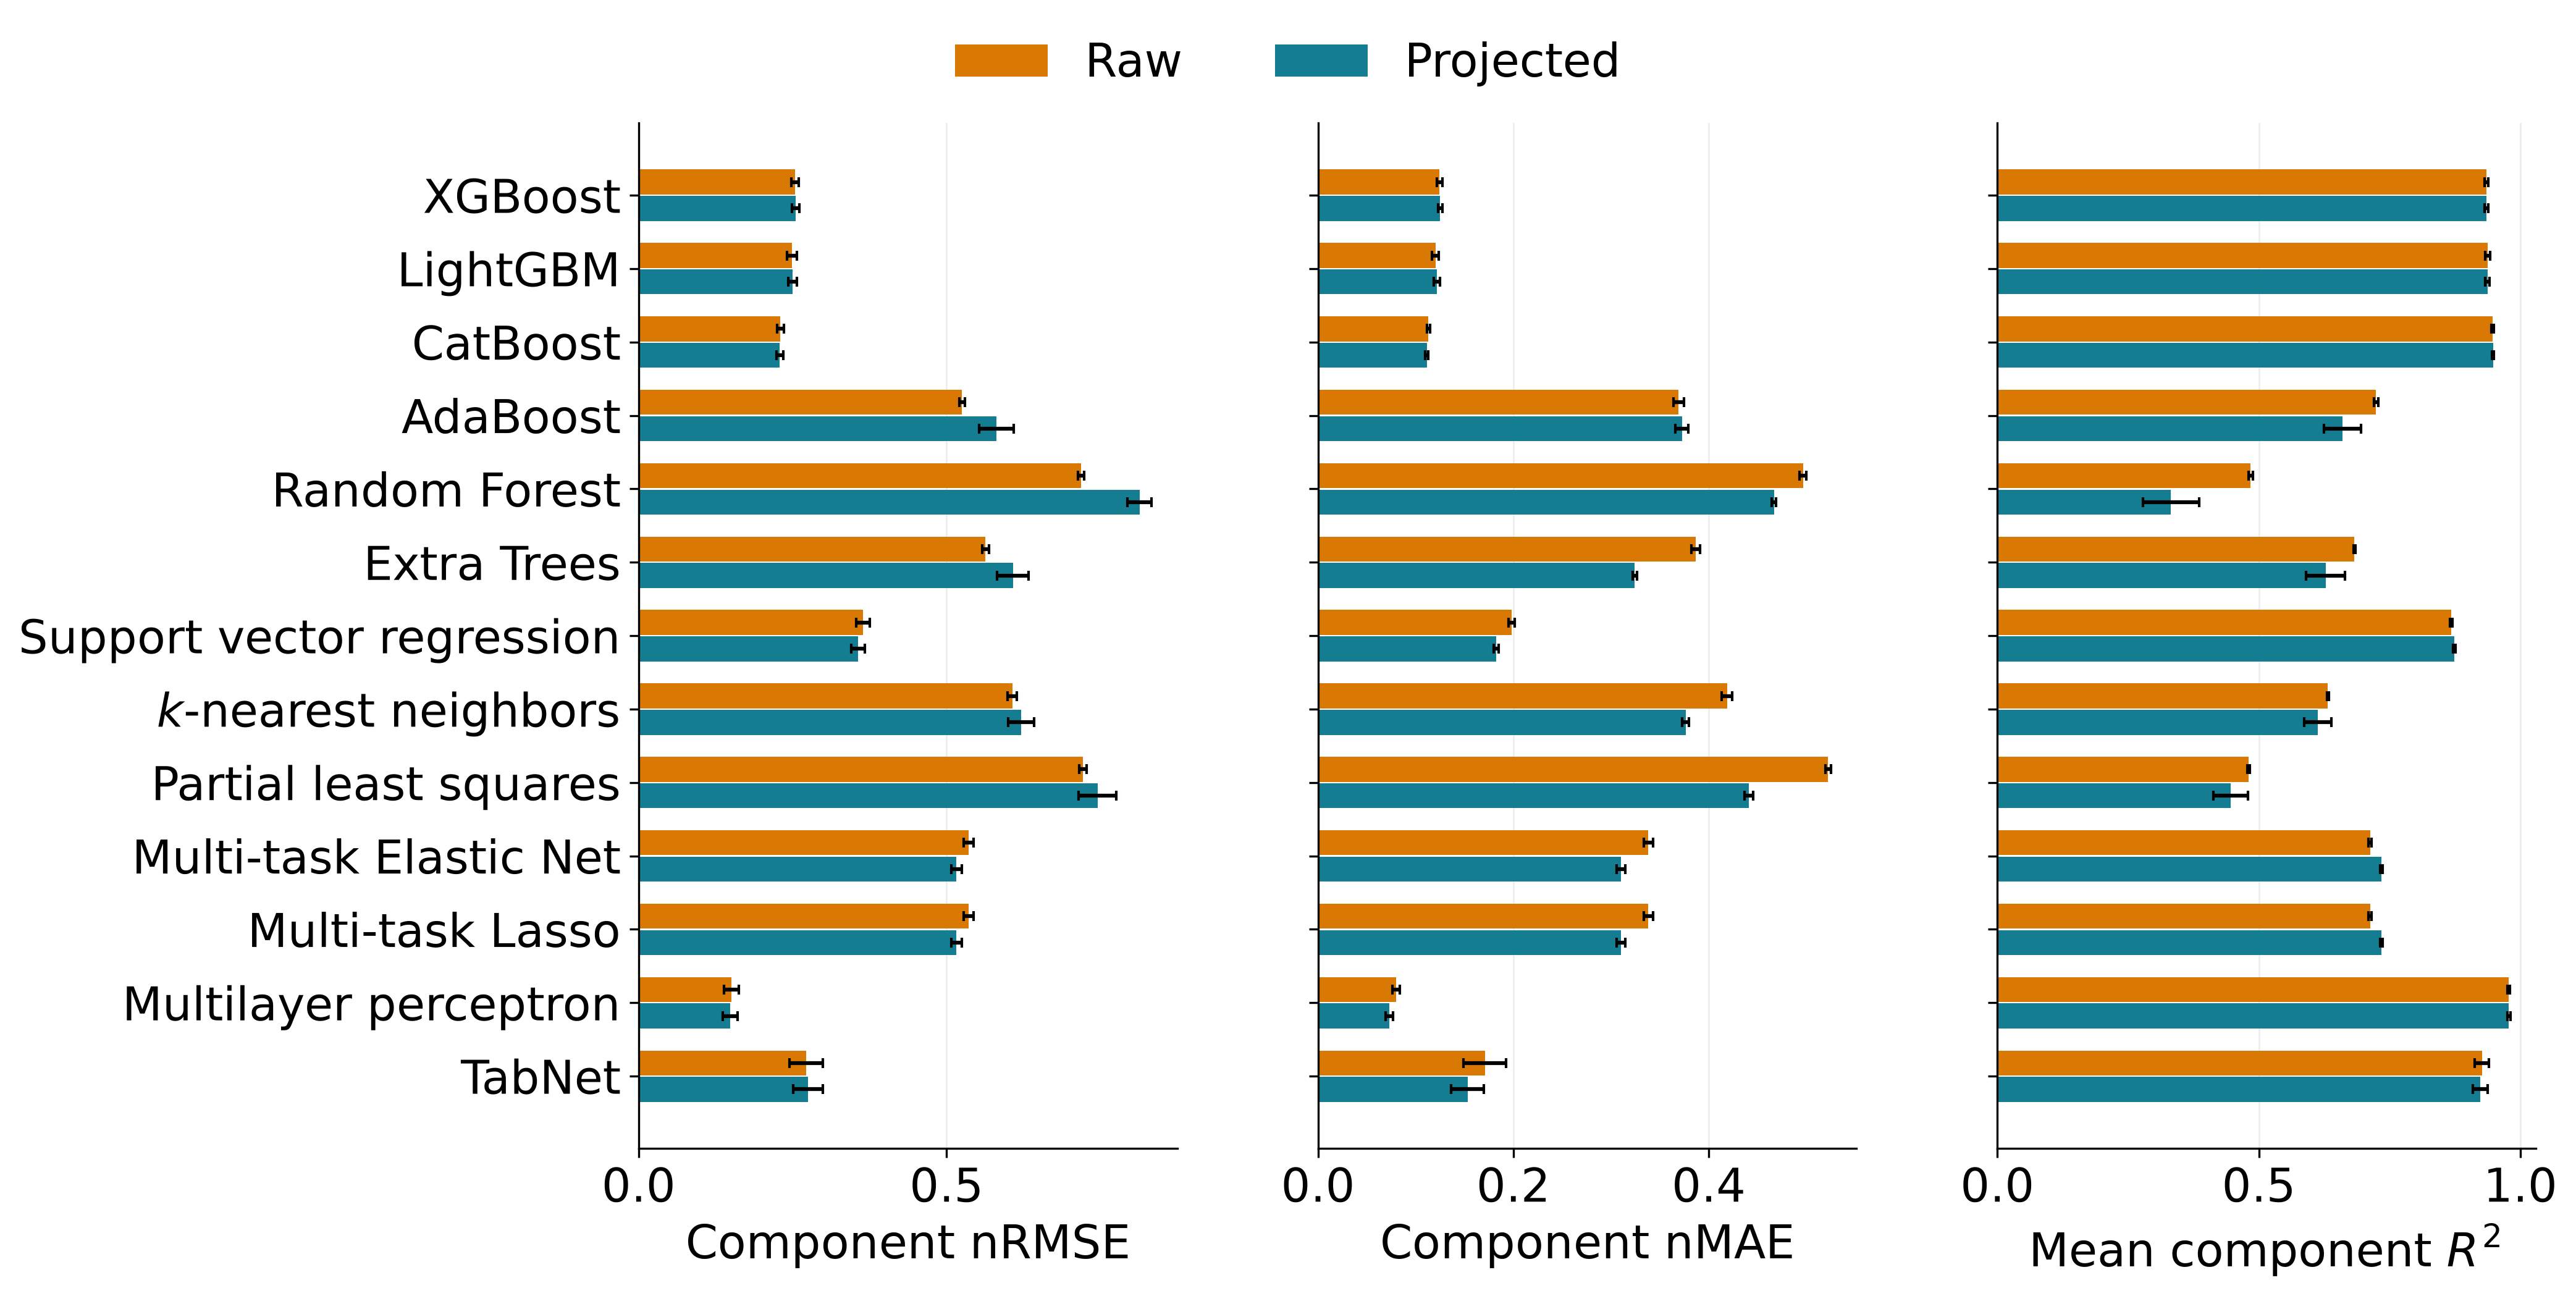
\includegraphics[width=\textwidth]{results/ch4/q01_prediction_accuracy.png}
\caption{Raw and projected component accuracy at $N=10{,}000$. Panels show nRMSE, nMAE, and the mean component $R^2$. Error bars show one sample standard deviation across five outer folds.}
\label{fig:projection_accuracy_results}
\end{figure}

\subsection{Response to the amount of training data}

Every predictor had lower raw nRMSE at $N=10{,}000$ than at $N=500$. Figure~\ref{fig:projection_learning_results} shows the complete trajectories. XGBoost and LightGBM had the lowest observed mean raw errors at $N=500$, with values of 0.435 and 0.439. The multilayer perceptron improved from 0.524 to 0.150. TabNet improved from 0.938 to 0.272 and showed the largest endpoint reduction among the predictors.

\begin{figure}[htbp]
\centering
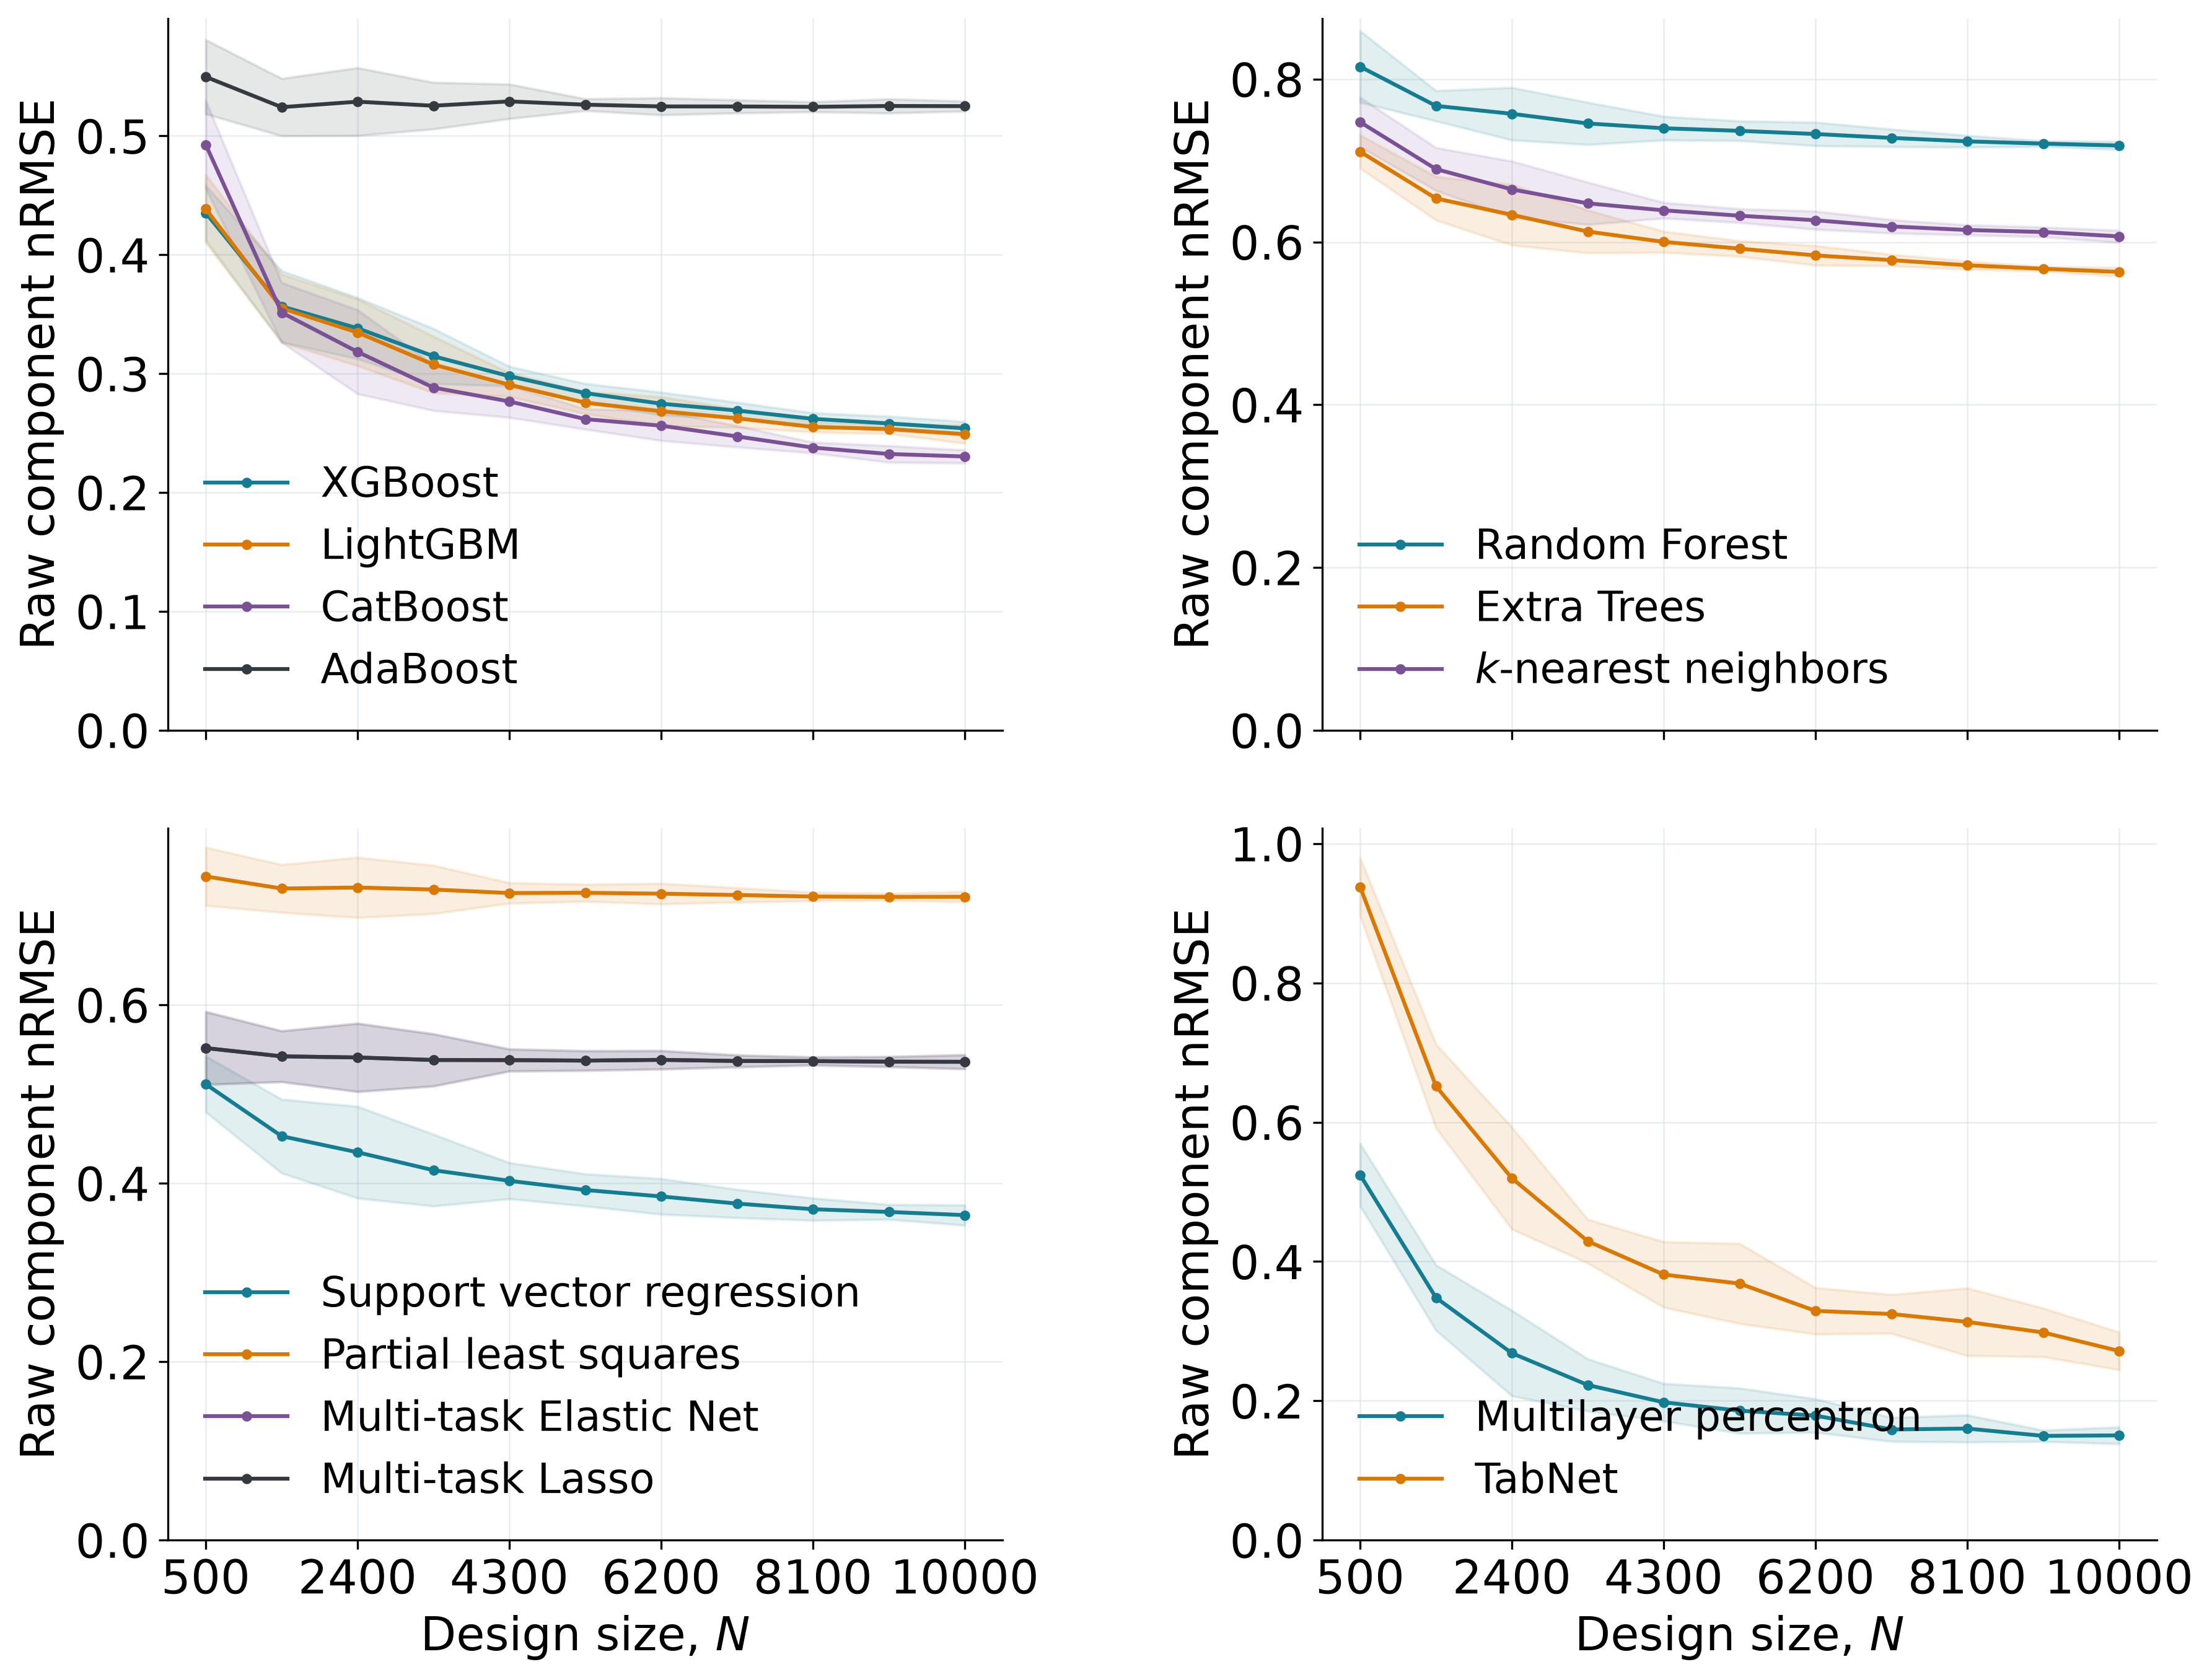
\includegraphics[width=\textwidth]{results/ch4/q02_learning_curves.png}
\caption{Raw component prediction error across the eleven nested design sizes. Separate panels group the predictors by their response representation. Lines show the five-fold mean nRMSE. Shaded regions show one sample standard deviation across folds.}
\label{fig:projection_learning_results}
\end{figure}

The lowest-error predictor changed with the data budget. The boosted trees performed well at the smallest design size. The multilayer perceptron attained the lowest error at the largest size. TabNet still improved from 0.298 at $N=9050$ to 0.272 at $N=10{,}000$. Its final reduction was approximately 0.0266. Its error continued to decrease at the largest evaluated sizes.

The effect of projection also varied with design size. Both multi-task linear models benefited at all eleven sizes. Support vector regression benefited at every size from $N=5250$ onward. The projection effect for the multilayer perceptron and TabNet changed sign across the size sequence. These trajectories were obtained with the prescribed fold-specific settings selected at the largest size.

Figure~\ref{fig:projection_size_effect_results} separates this adjustment effect from the raw learning curves. A negative cell indicates lower error after projection. The persistent reductions for the multi-task models contrast with the mixed effects for the more flexible predictors.

\begin{figure}[htbp]
\centering
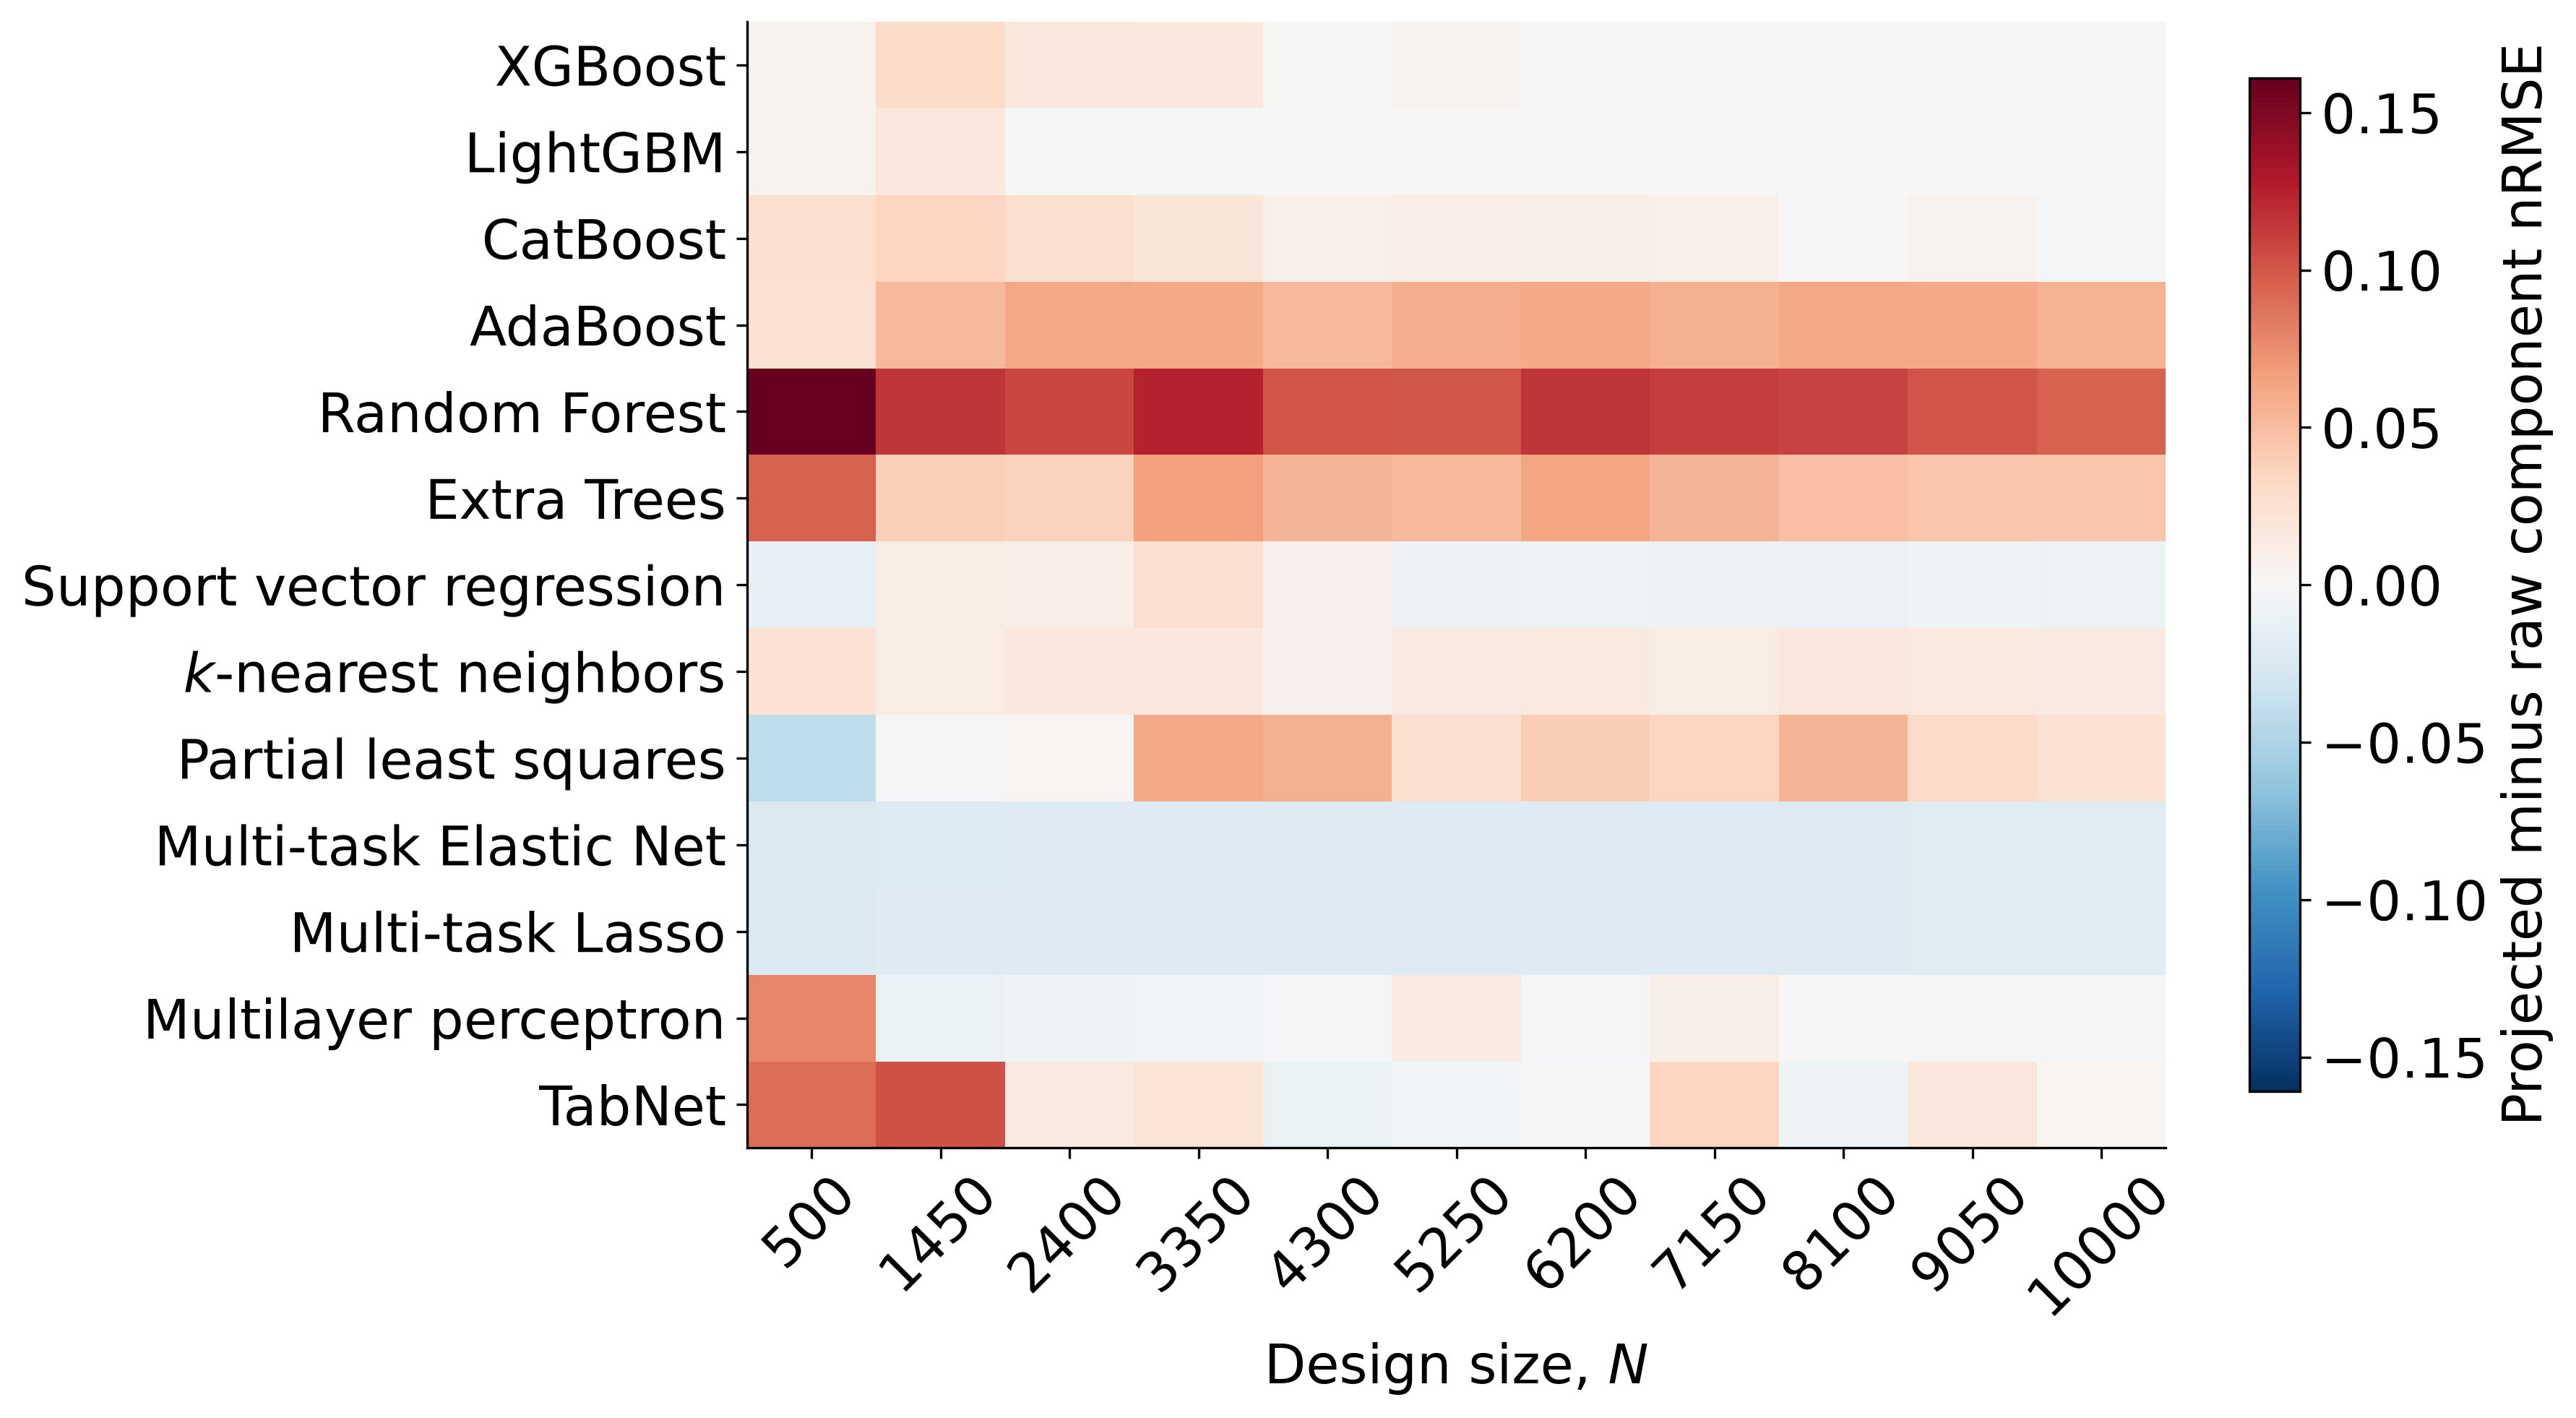
\includegraphics[width=\textwidth]{results/ch4/q03_projection_effect.png}
\caption{Projected minus raw mean component nRMSE for every predictor and design size. Negative values indicate improvement. Both prediction types use the same assessment folds and training-defined component scales.}
\label{fig:projection_size_effect_results}
\end{figure}

\subsection{Physical enforcement and component redistribution}

Every raw assessment state failed the declared mass conservation tolerance at every design size. At $N=10{,}000$, AdaBoost, Random Forest, Extra Trees, and the nearest-neighbor predictor nevertheless returned only non-negative raw concentrations. The other predictors had row-level non-negativity violation rates from 39.0\% to 76.8\%. Table~\ref{tab:projection_constraint_results} reports their rates and the size of the subsequent adjustment.

\begin{table}[htbp]
\centering\small
\caption{Physical diagnostics at $N=10{,}000$. Entries are five-fold means. Every raw mass conservation violation rate was 100\%. Every projected mass conservation and non-negativity violation rate was zero.}
\label{tab:projection_constraint_results}
\begin{tabular}{p{4.2cm}rrr}
\toprule
Surrogate & \begin{tabular}{r}Raw negative\\states (\%)\end{tabular} & \begin{tabular}{r}Interpolation\\activated (\%)\end{tabular} & Mean $d_c^{\mathrm{std}}$\\
\midrule
XGBoost & 39.72 & 0.00 & 0.300\\
LightGBM & 38.95 & 0.00 & 0.301\\
CatBoost & 59.06 & 0.00 & 0.242\\
AdaBoost & 0.00 & 0.30 & 0.901\\
Random Forest & 0.00 & 1.42 & 2.002\\
Extra Trees & 0.00 & 0.88 & 1.528\\
Support vector regression & 76.78 & 0.01 & 0.363\\
$k$-nearest neighbors & 0.00 & 0.25 & 1.192\\
Partial least squares & 54.31 & 0.93 & 1.808\\
Multi-task Elastic Net & 71.06 & 0.00 & 0.482\\
Multi-task Lasso & 71.05 & 0.00 & 0.482\\
Multilayer perceptron & 58.58 & 0.00 & 0.189\\
TabNet & 60.48 & 0.04 & 0.545\\
\bottomrule
\end{tabular}
\end{table}

Projection produced no mass conservation or non-negativity failures in the 750,750 prediction instances evaluated across all thirteen predictors and eleven design sizes. These prediction instances include repeated assessment across nested sizes. The maximum projected invariant residual was $2.06\times10^{-13}$. Interpolation for non-negativity was activated in 2489 instances, or 0.332\%. Random Forest, partial least squares, and Extra Trees accounted for 904, 574, and 566 activations, respectively. Together they accounted for 82.1\% of the activations.

Figure~\ref{fig:projection_physical_results} compares negative raw states with adjustment size and interpolation use. These are separate properties. Random Forest had no negative raw states but required the largest mean displacement and the most frequent interpolation at the largest design size.

\begin{figure}[htbp]
\centering
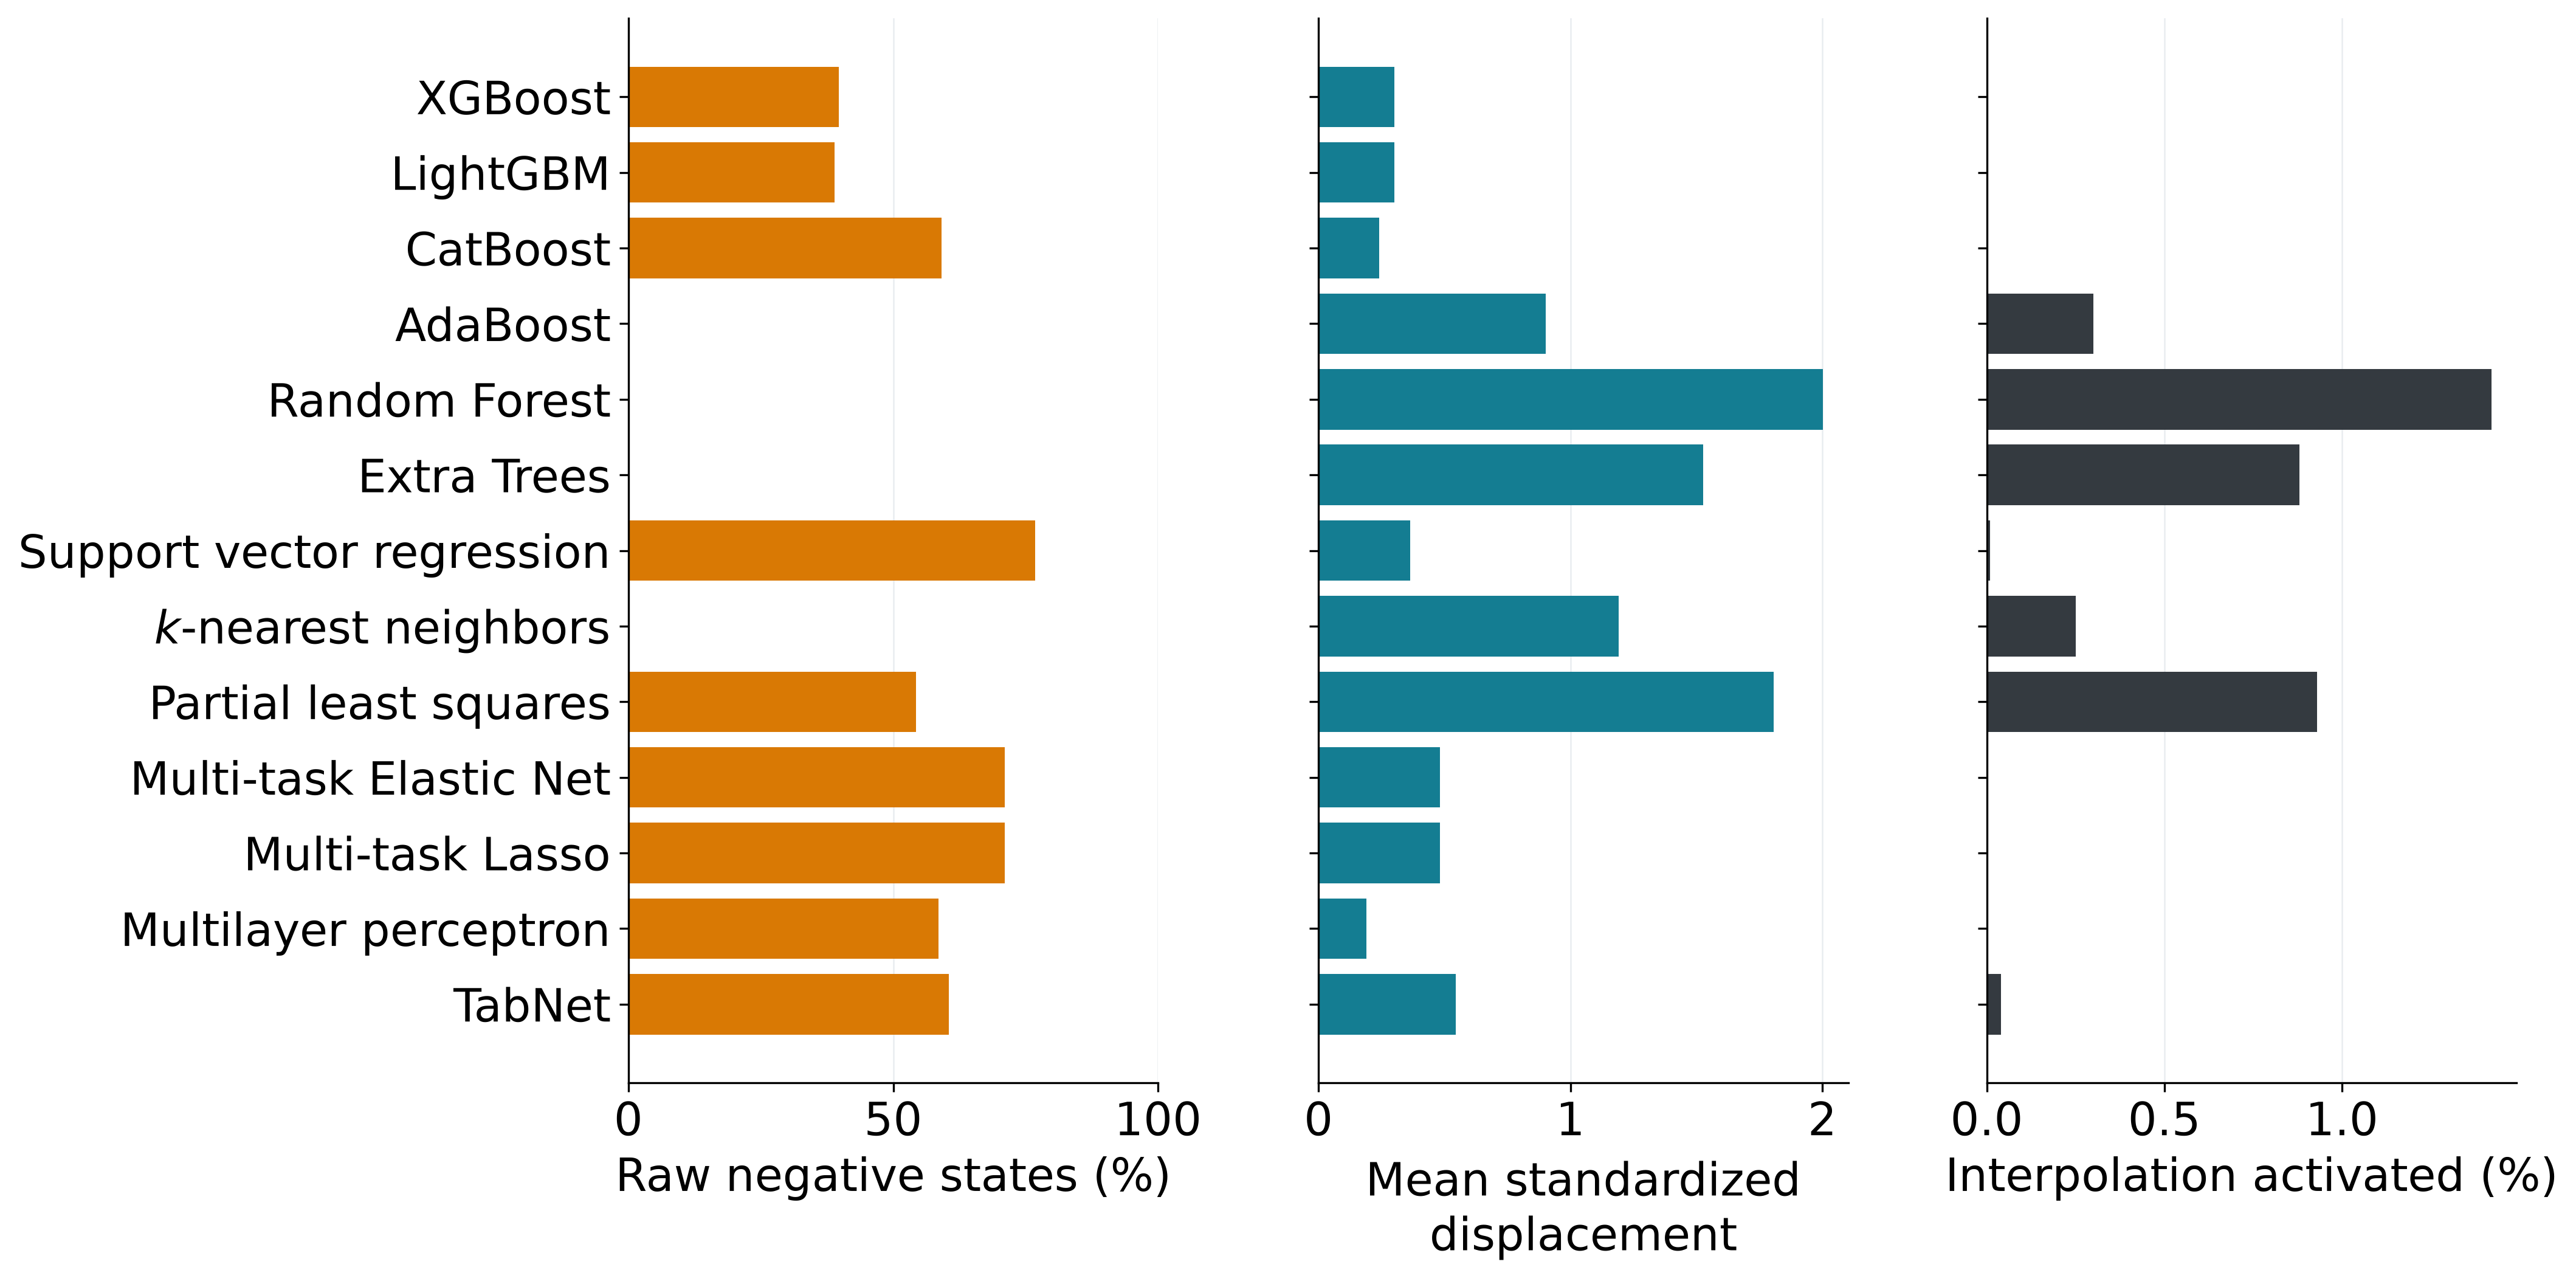
\includegraphics[width=\textwidth]{results/ch4/q04_physical_compliance.png}
\caption{Physical diagnostics at $N=10{,}000$. Panels show the fraction of raw states with negative components, mean standardized displacement, and interpolation activation. Values are five-fold means. All raw states failed the mass conservation tolerance, while every projected state passed both imposed physical checks.}
\label{fig:projection_physical_results}
\end{figure}

At the largest design size, projection reduced component nRMSE in 188 of the 260 predictor--component comparisons. Both multi-task linear models improved eighteen of twenty components. The multilayer perceptron improved seventeen. CatBoost, partial least squares, and support vector regression each improved sixteen. In contrast, the heterotrophic biomass component $X_H$ had higher error for every predictor. Random Forest's fermentable-substrate component $S_F$ increased from nRMSE 0.887 to 1.993. Its 142 interpolated predictions accounted for that component's error increase, while the other 9858 predictions retained essentially the same squared error.

Figure~\ref{fig:projection_component_results} locates the component-level changes. The larger positive changes in a few components explain why an aggregate squared-error measure can increase even when most component scores improve.

\begin{figure}[htbp]
\centering
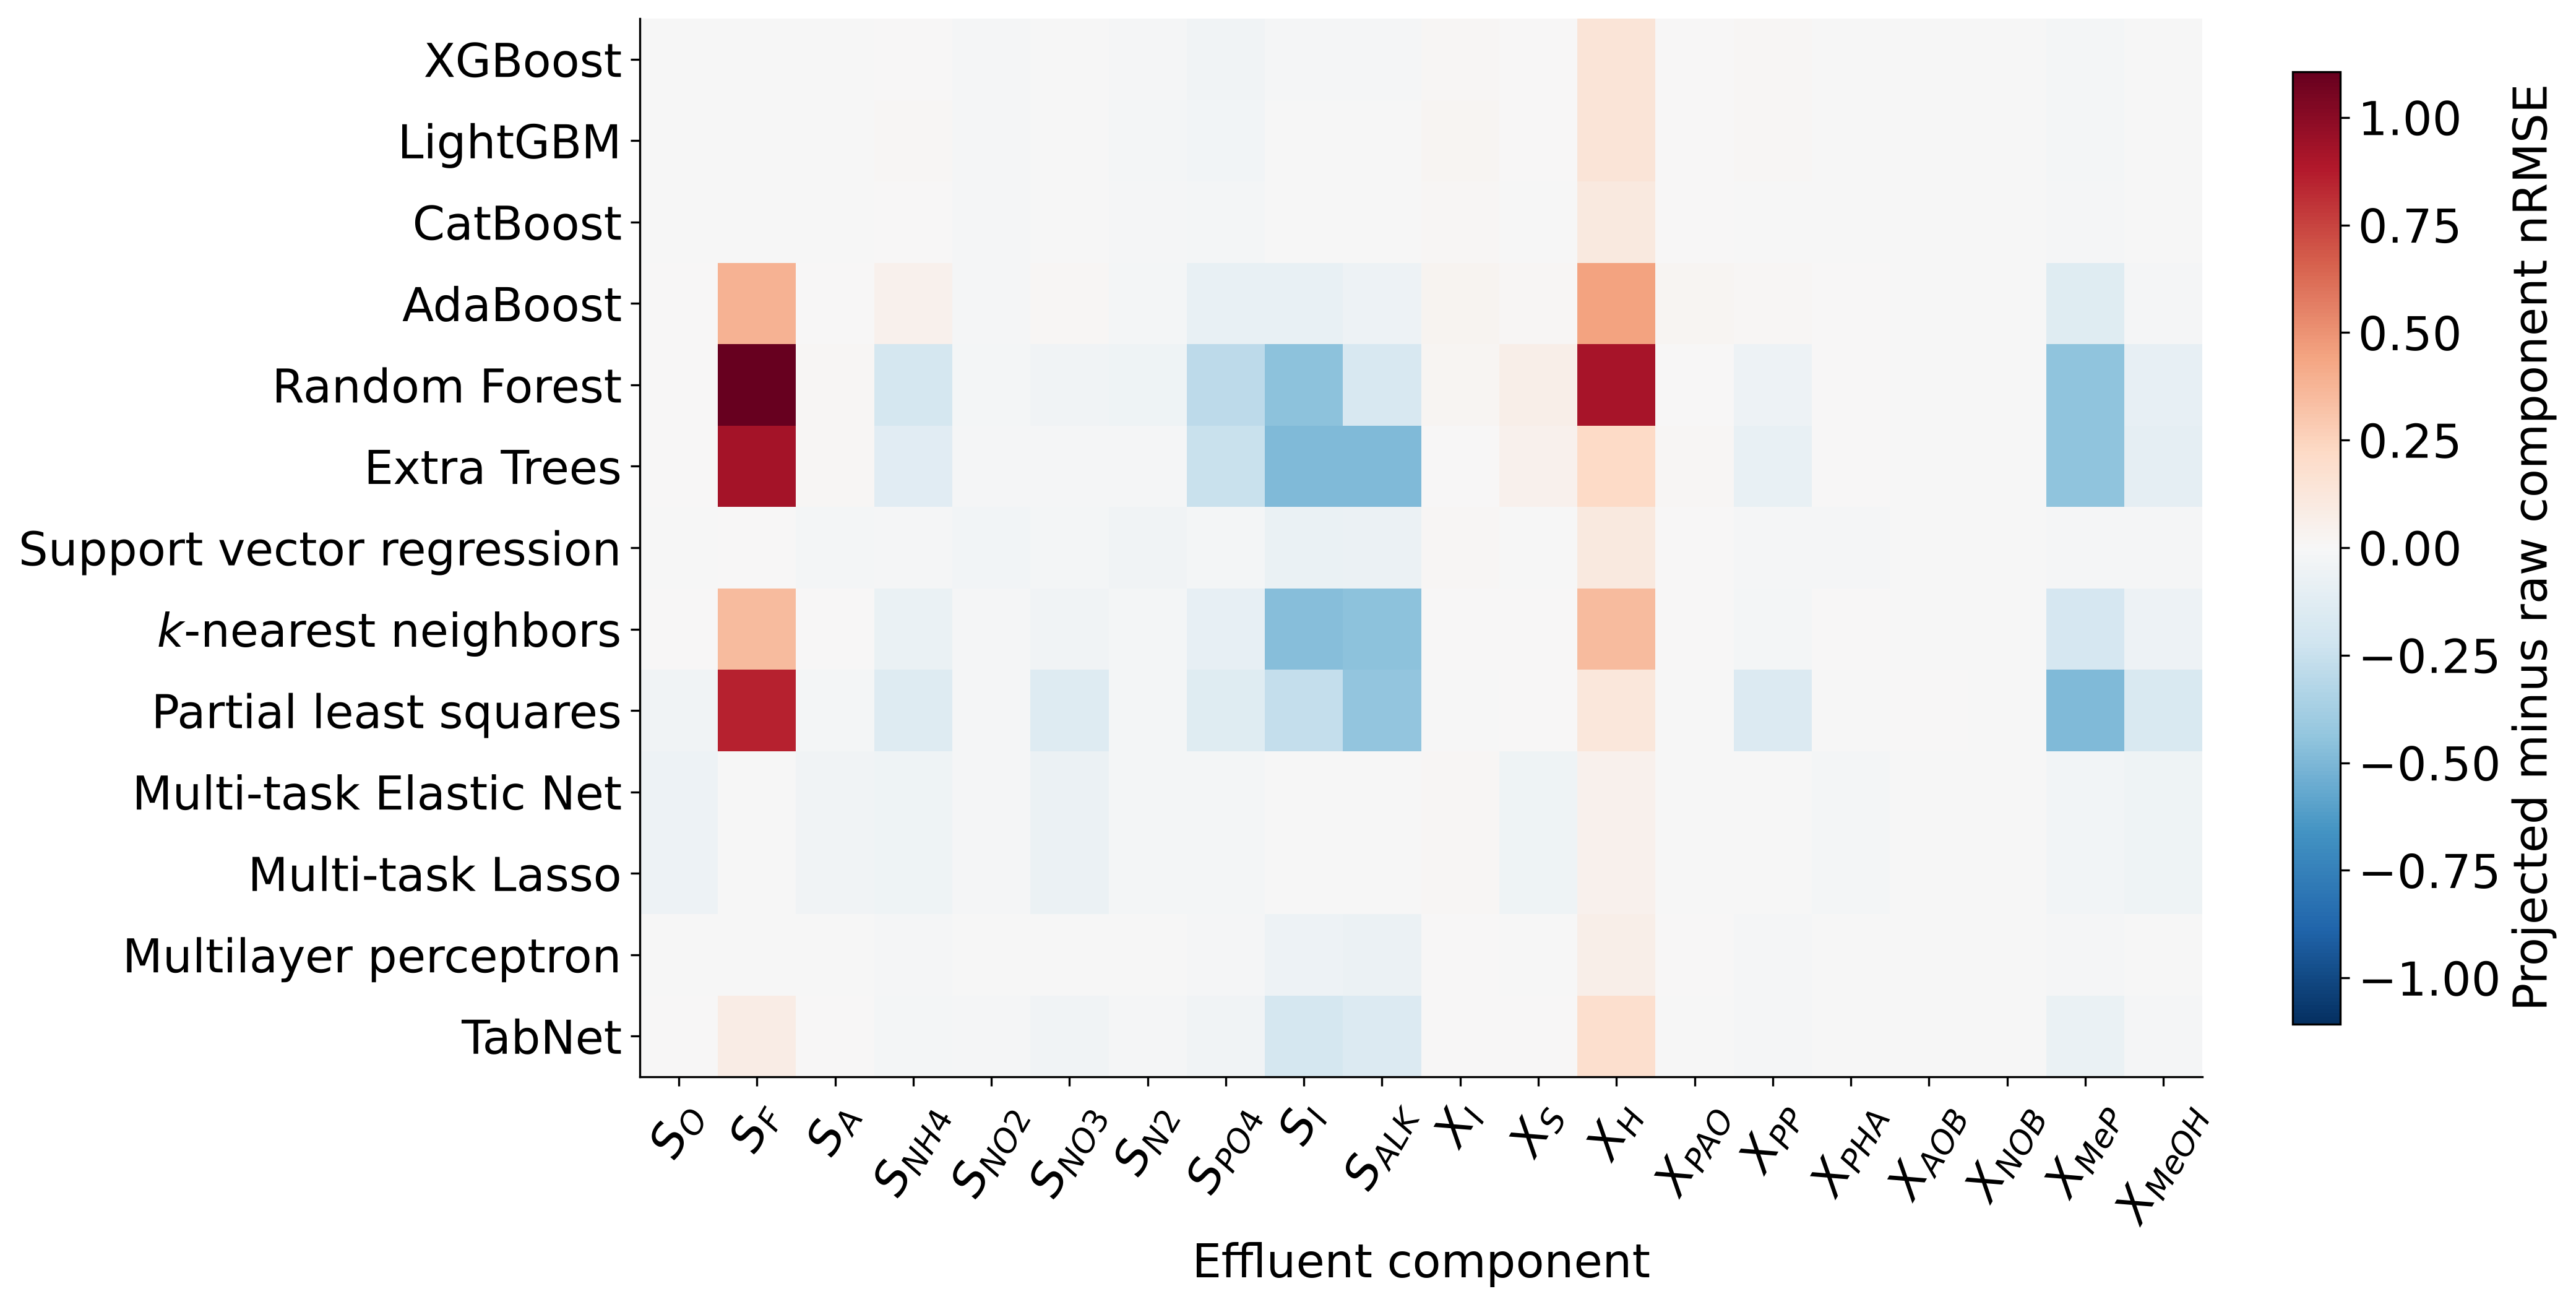
\includegraphics[width=\textwidth]{results/ch4/q05_component_error_change.png}
\caption{Projected minus raw component nRMSE at $N=10{,}000$. Each cell is the difference between five-fold mean scores for one predictor and one component. Negative values indicate improvement. The same color limits apply to all cells.}
\label{fig:projection_component_results}
\end{figure}

The composite results also differed by quantity. Every predictor had lower TN and TP normalized root error after projection. Every predictor had higher COD and TSS normalized root error. The reported composites therefore responded differently to the same component adjustment.

Figure~\ref{fig:projection_composite_results} presents the corresponding root errors in physical units. TN and TP improved while COD and TSS worsened for every predictor. The component projection thus changed the accuracy of different reporting quantities in different directions.

\begin{figure}[htbp]
\centering
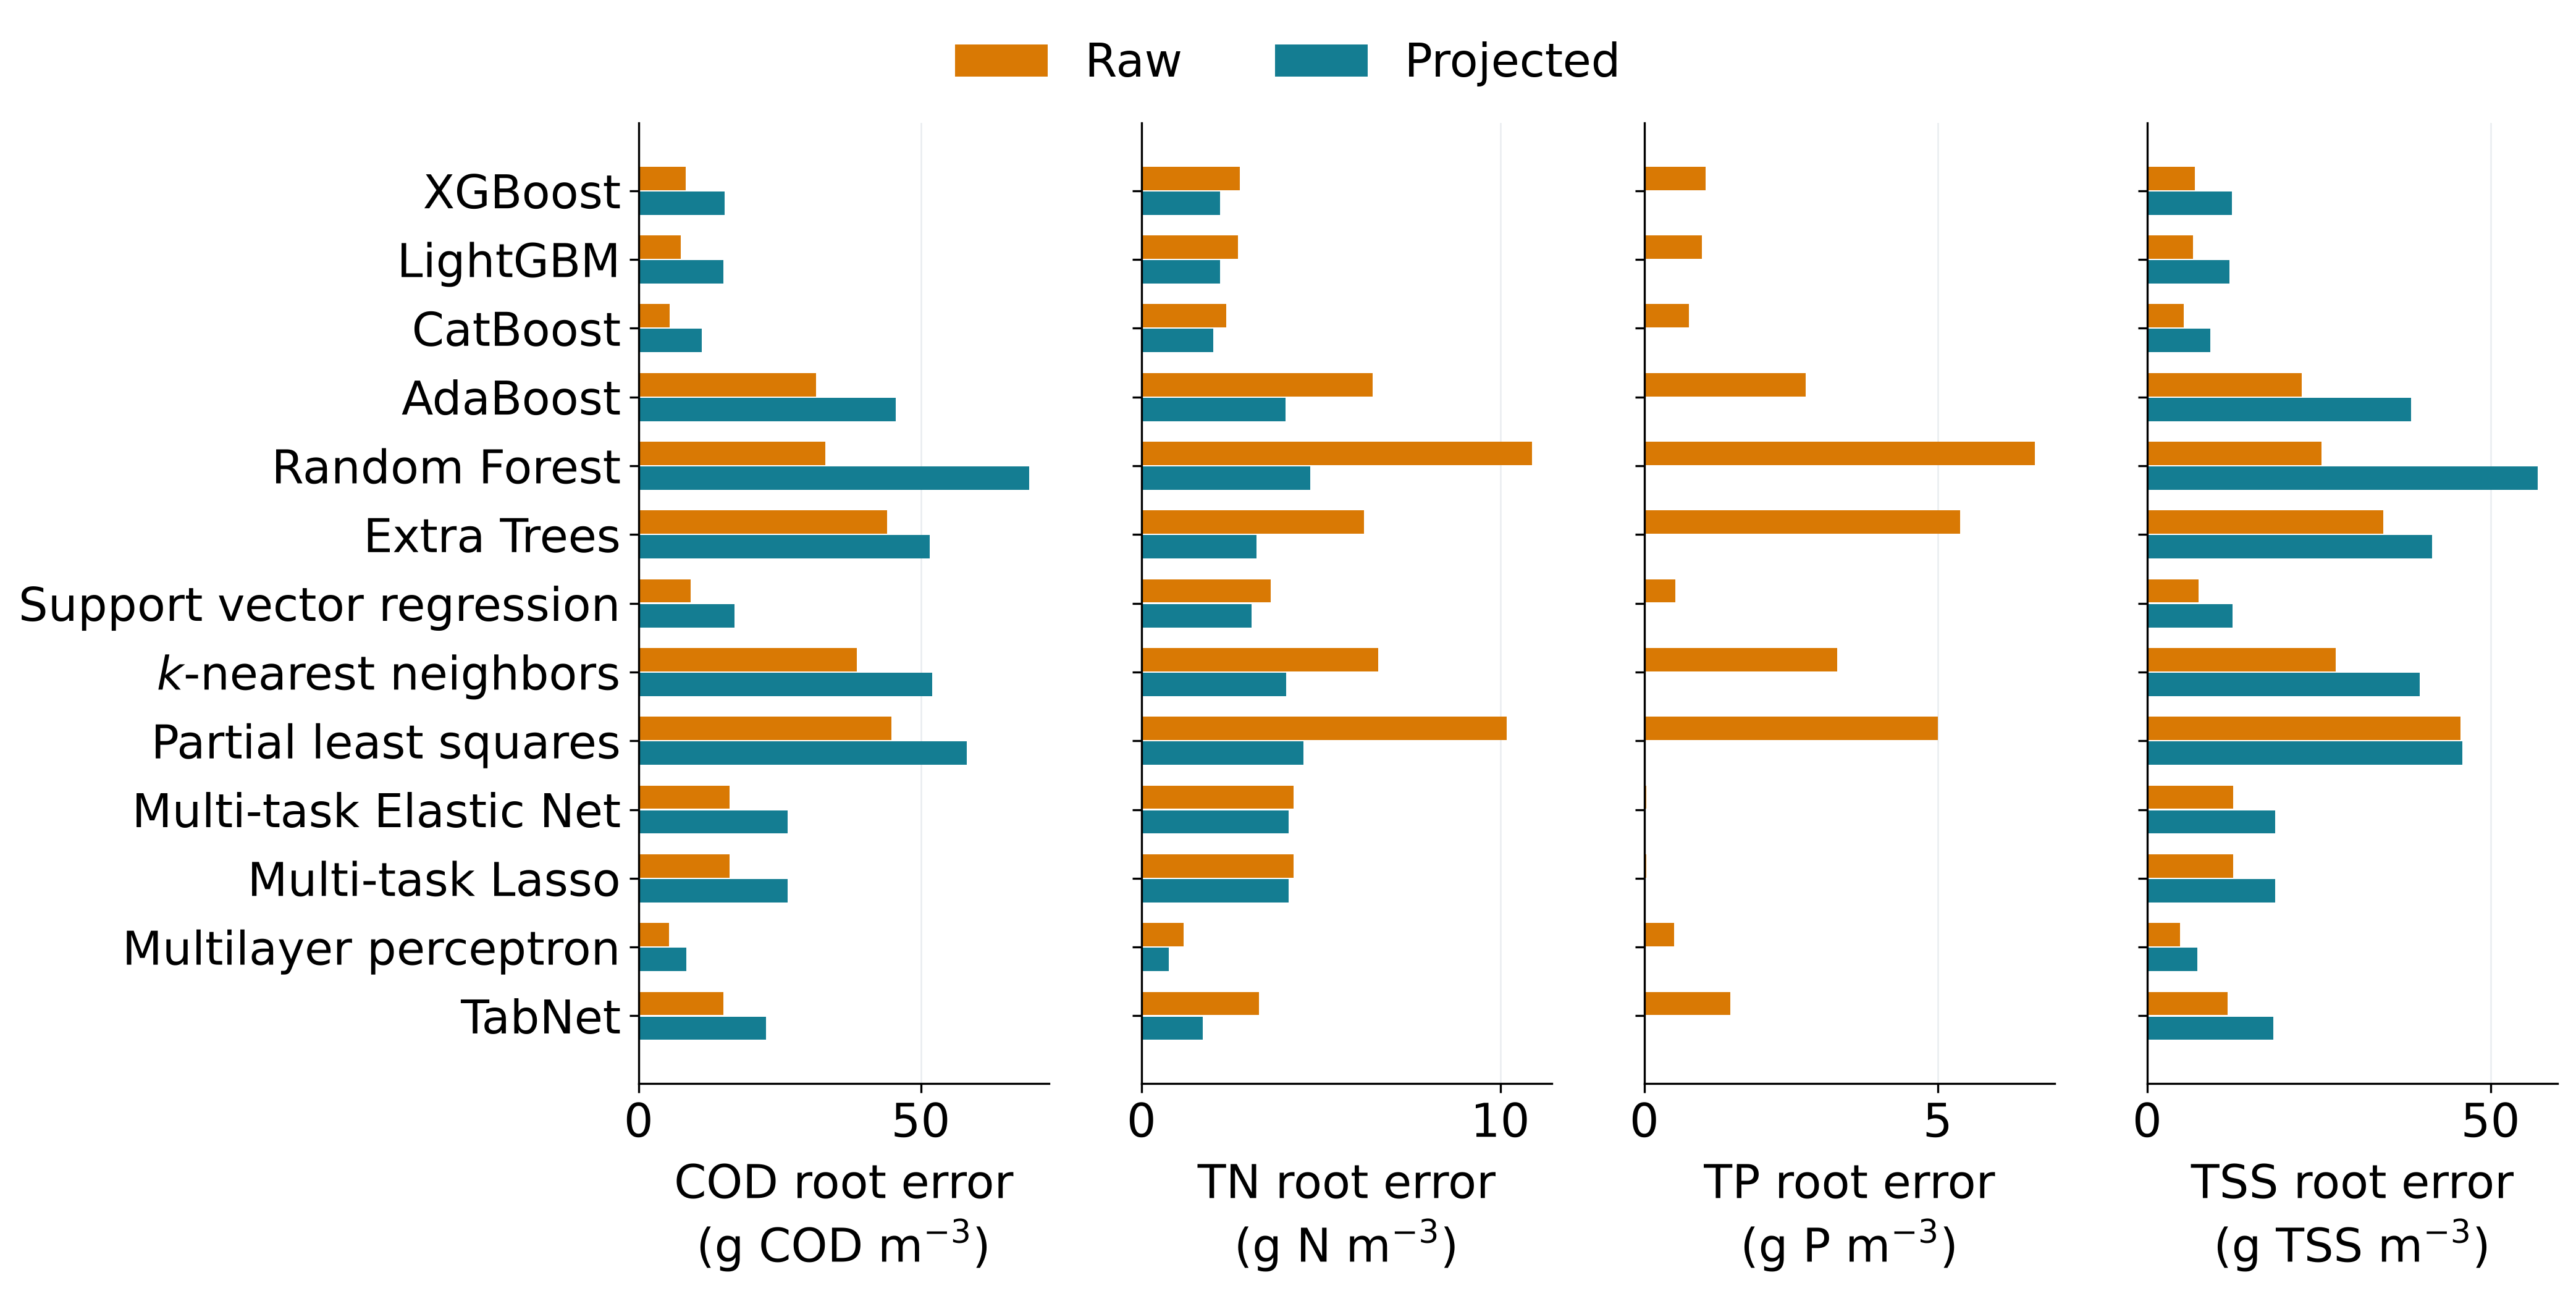
\includegraphics[width=\textwidth]{results/ch4/q06_composite_error_change.png}
\caption{Raw and projected root mean squared errors for COD, TN, TP, and TSS at $N=10{,}000$. Bars show means of five fold-specific root errors. Each panel uses the physical unit of its own reported quantity. These errors are distinct from the standardized component nRMSE.}
\label{fig:projection_composite_results}
\end{figure}

\subsection{Prediction beyond the learning domain}

Both raw and projected error increased from mild to severe exterior inputs for every predictor. The multilayer perceptron had the lowest error in both designs. Its projected nRMSE was 0.251 for mild inputs and 0.521 for severe inputs. TabNet followed at 0.333 and 0.547. Table~\ref{tab:projection_exterior_results} reports the full comparison under the common full-domain normalization.

\begin{table}[htbp]
\centering\small
\caption{Component nRMSE beyond the learning domain. Each entry summarizes 600 accepted mechanistic states from one full-domain refit. }
\label{tab:projection_exterior_results}
\begin{tabular}{p{4.5cm}rrrr}
\toprule
& \multicolumn{2}{c}{Mild exterior inputs} & \multicolumn{2}{c}{Severe exterior inputs}\\
Surrogate & Raw & Projected & Raw & Projected\\
\midrule
XGBoost & 0.424 & 0.420 & 0.861 & 0.853\\
LightGBM & 0.419 & 0.413 & 0.848 & 0.842\\
CatBoost & 0.393 & 0.387 & 0.836 & 0.828\\
AdaBoost & 0.692 & 0.711 & 1.036 & 1.139\\
Random Forest & 0.908 & 0.996 & 1.242 & 1.489\\
Extra Trees & 0.717 & 0.679 & 1.084 & 1.222\\
Support vector regression & 0.555 & 0.538 & 0.989 & 0.948\\
$k$-nearest neighbors & 0.760 & 0.732 & 1.113 & 1.147\\
Partial least squares & 0.908 & 0.841 & 1.267 & 1.190\\
Multi-task Elastic Net & 0.750 & 0.688 & 1.146 & 1.044\\
Multi-task Lasso & 0.751 & 0.688 & 1.146 & 1.044\\
Multilayer perceptron & 0.255 & 0.251 & 0.531 & 0.521\\
TabNet & 0.336 & 0.333 & 0.563 & 0.547\\
\bottomrule
\end{tabular}
\end{table}

Projection reduced aggregate nRMSE in eleven of thirteen mild comparisons and nine of thirteen severe comparisons. AdaBoost and Random Forest worsened in both designs. Extra Trees and the nearest-neighbor predictor also worsened in the severe design. Component error decreased in 192 of 260 mild comparisons and 193 of 260 severe comparisons. Every predictor improved a majority of its component scores in each exterior design.

Figure~\ref{fig:projection_exterior_results} uses a common horizontal scale for the two severity levels. The larger severe-domain errors remain visible even for the most accurate predictors. Both prediction types had larger errors under severe exterior inputs.

\begin{figure}[htbp]
\centering
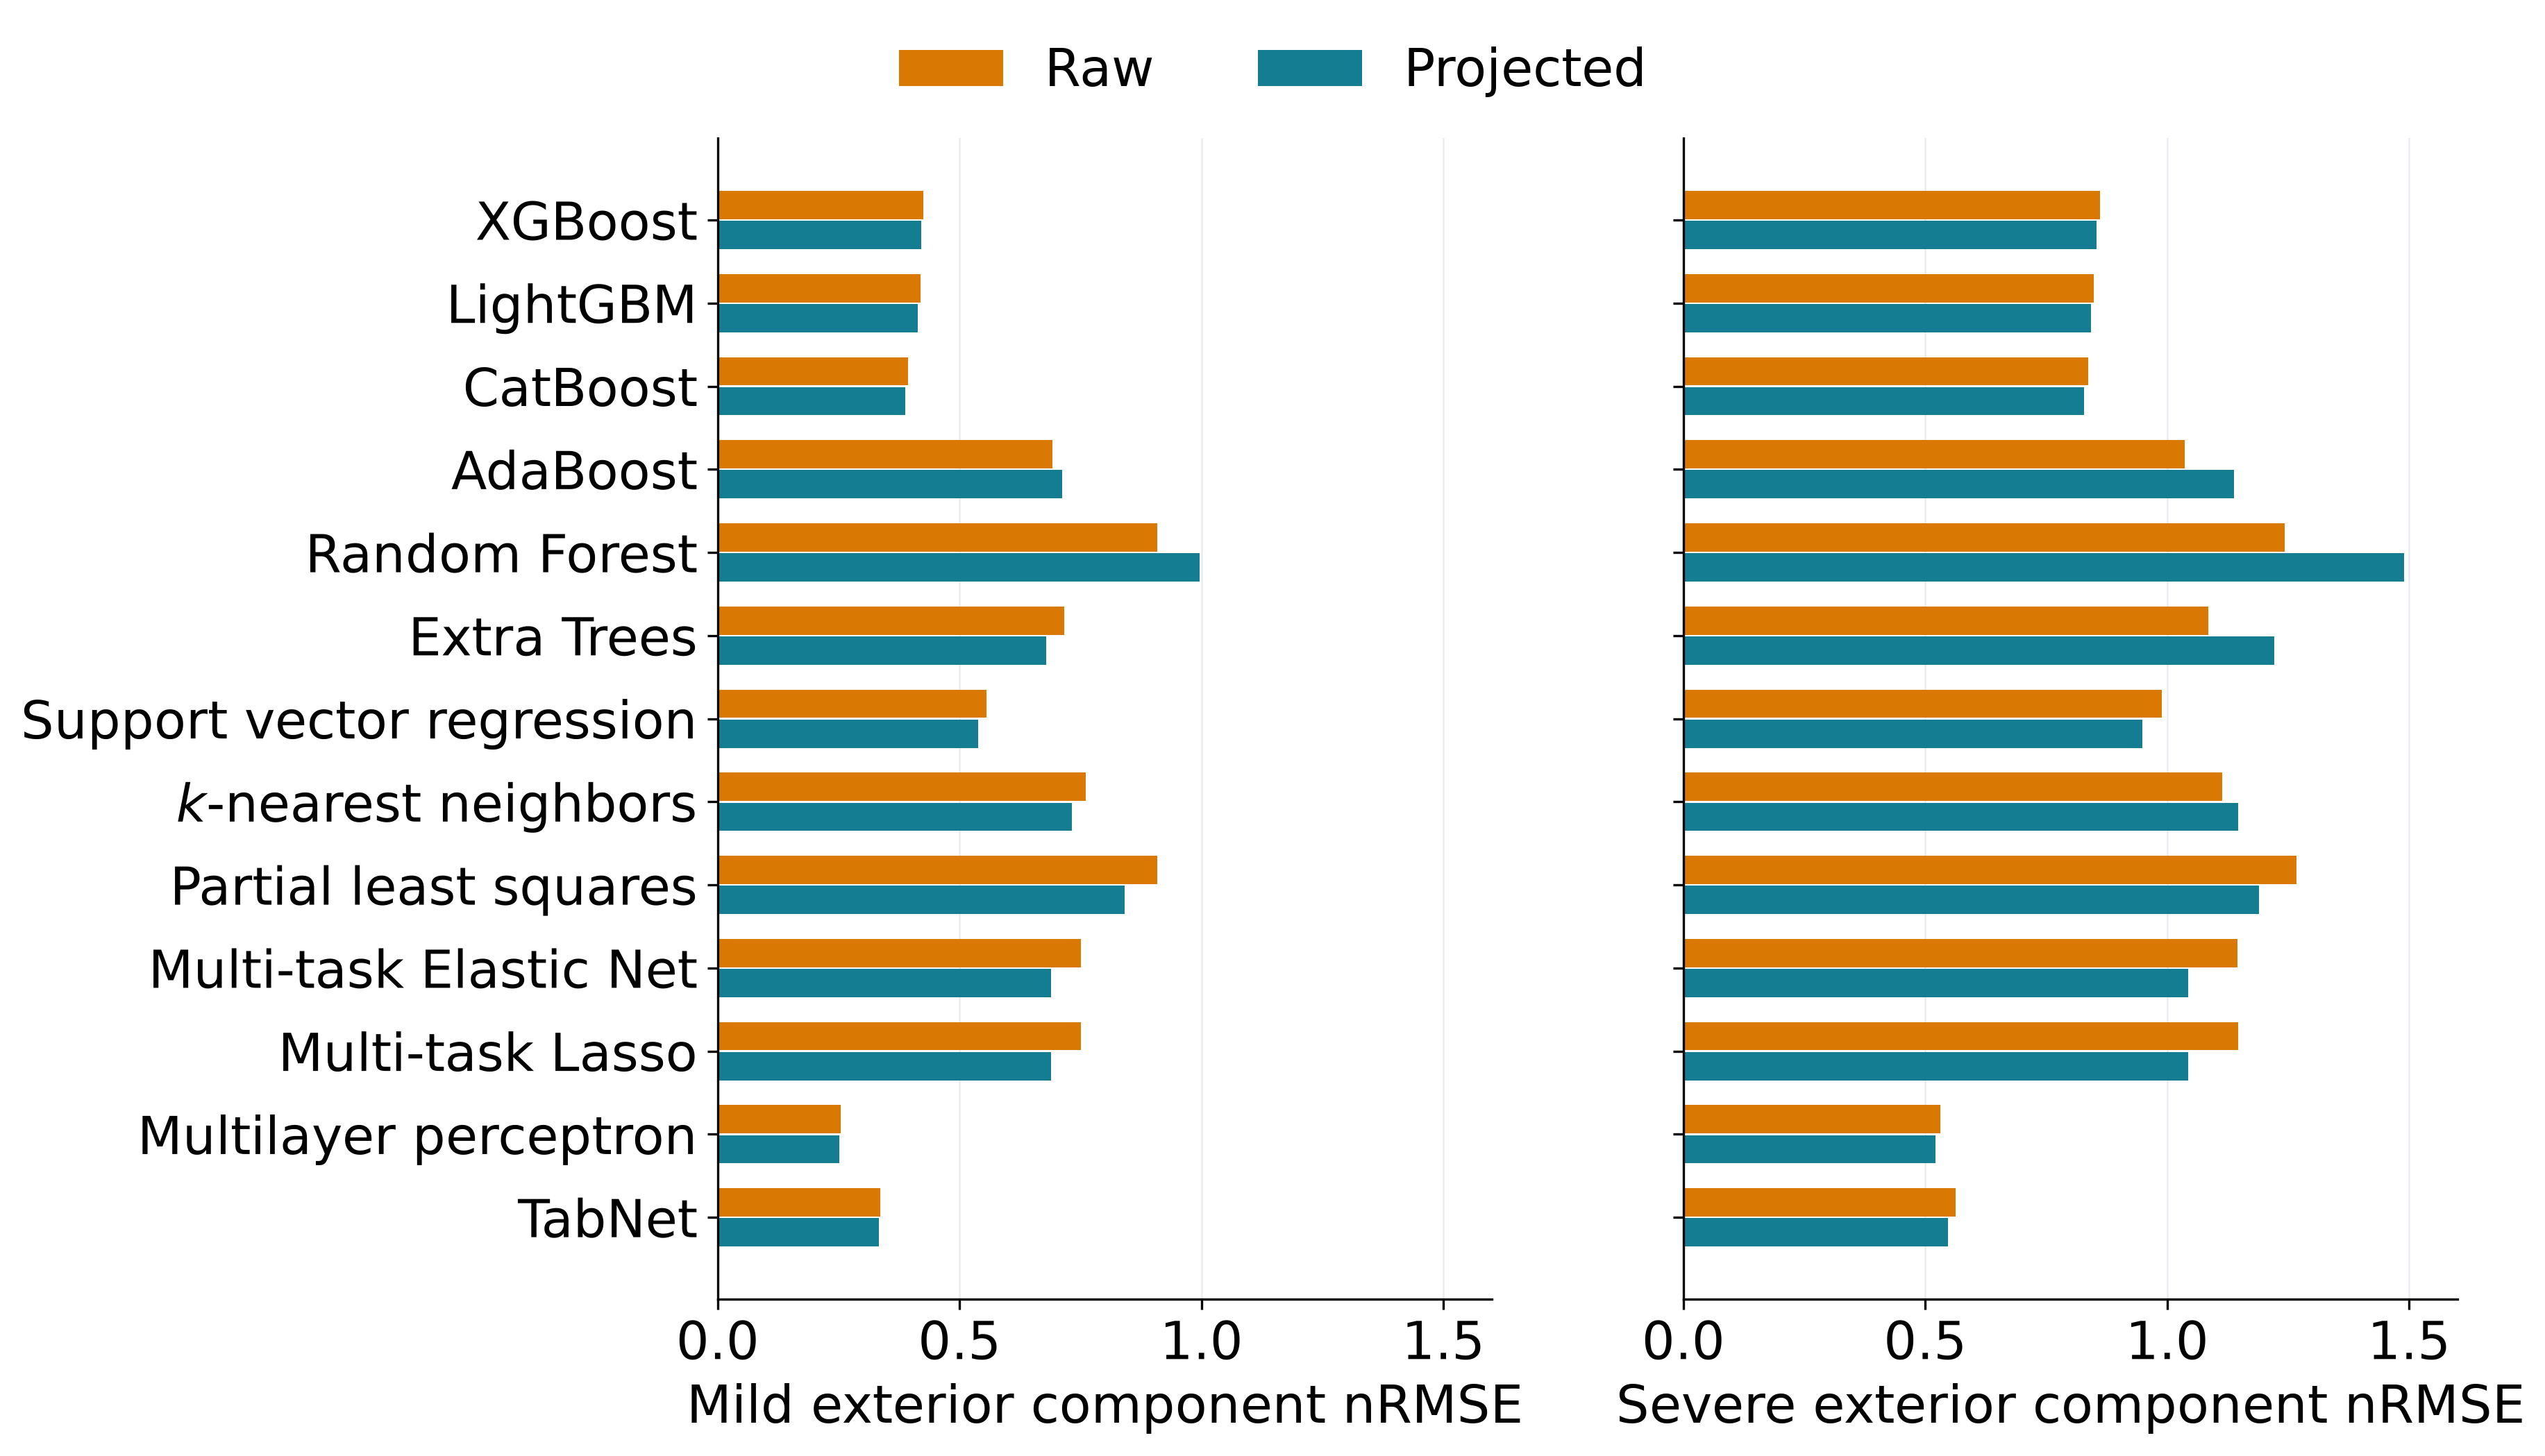
\includegraphics[width=\textwidth]{results/ch4/q07_exterior_accuracy.png}
\caption{Raw and projected component nRMSE for mild and severe exterior inputs. Each severity includes 600 independently simulated reference states. Both panels use full-domain training scales and a common error-axis range. }
\label{fig:projection_exterior_results}
\end{figure}

All 15,600 exterior projected prediction instances passed the imposed physical checks. Their maximum invariant residual was $1.72\times10^{-13}$. Interpolation was activated in 68 instances, or 0.436\%. Combining the interior and exterior assessments gave 766,350 projected prediction instances with no failures of the declared mass conservation and non-negativity checks. The increase in severe-domain error occurred despite this complete constraint compliance.

\subsection{Fitting and prediction costs}

Table~\ref{tab:projection_timing_results} separates model preparation from repeated prediction. At the largest design size, mean fitting time ranged from approximately 0.024 s for Multi-task Elastic Net to 56.02 s for support vector regression. Mean search time ranged from 14.21 s for Multi-task Lasso to 11,082.77 s for support vector regression. These preparation costs were incurred before repeated use of the fitted predictor.

Figure~\ref{fig:projection_cost_results} shows these differences on logarithmic axes. Projection dominated the inference cost of the fastest linear predictors. The two panels report preparation time and repeated prediction time separately.

\begin{figure}[htbp]
\centering
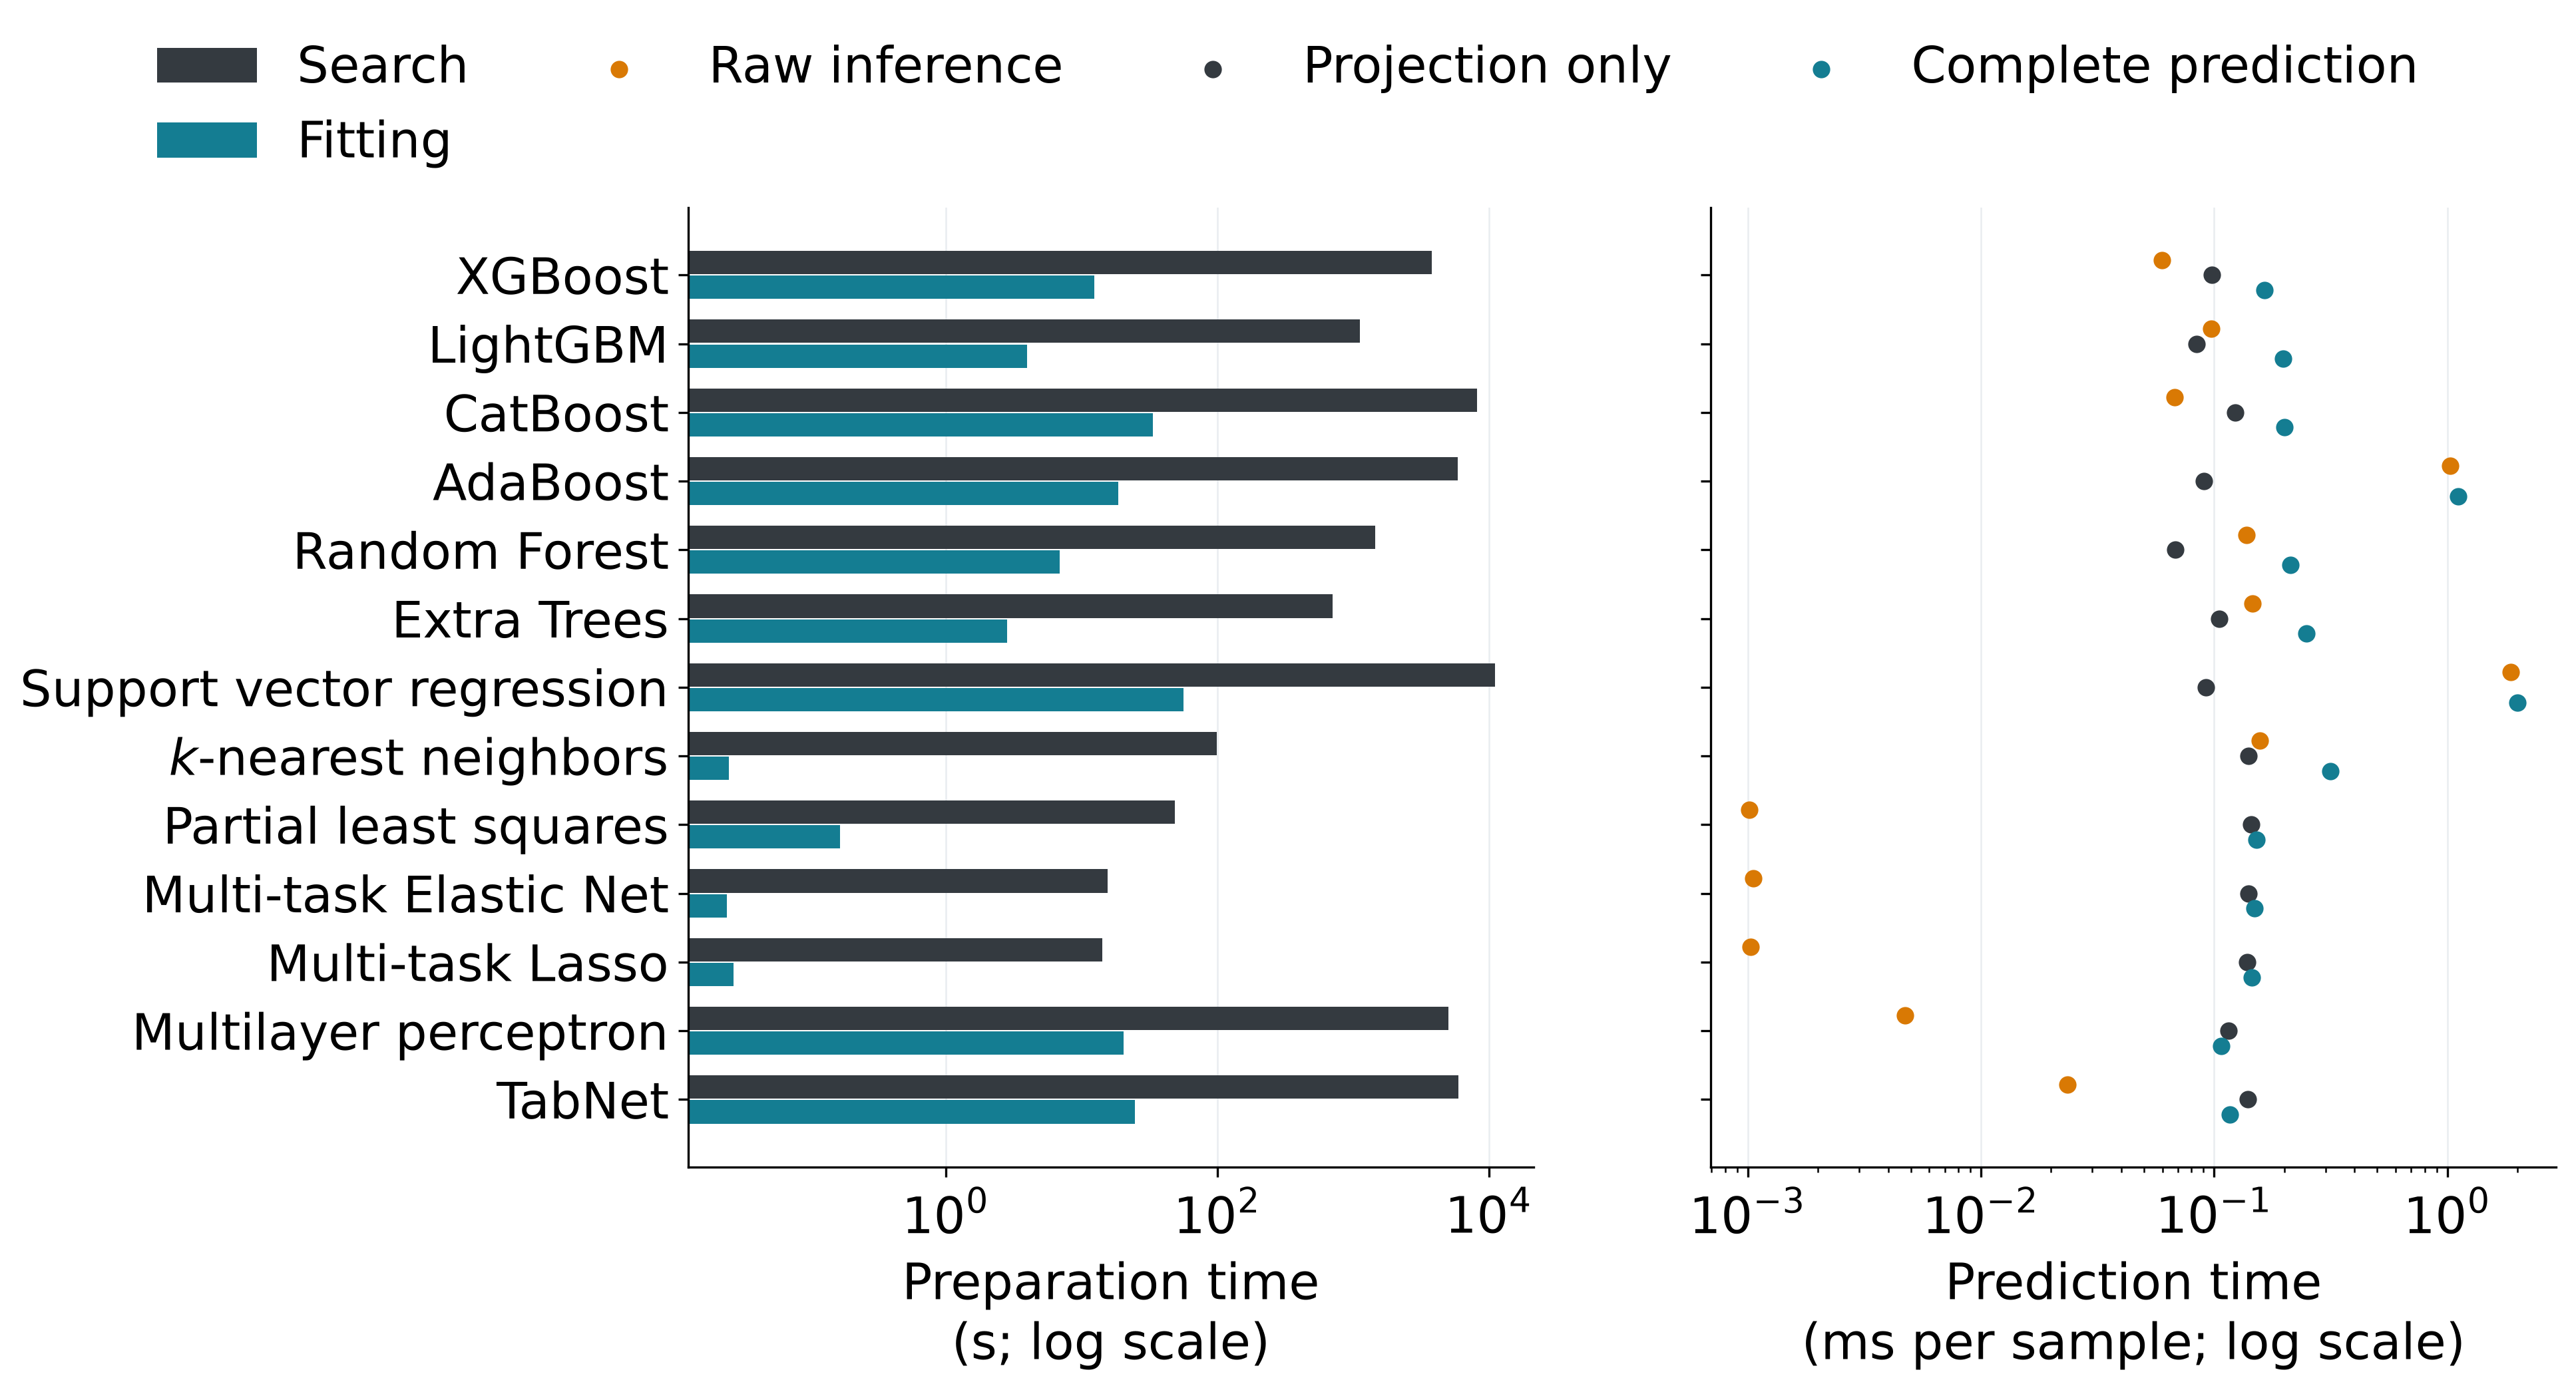
\includegraphics[width=\textwidth]{results/ch4/q08_computational_cost.png}
\caption{Model preparation and repeated prediction costs at $N=10{,}000$. The left panel separates search and fitting in seconds. The right panel separates raw inference, projection alone, and complete prediction in milliseconds per sample under the fixed batch protocol. Both panels show five-fold means on logarithmic axes. Complete prediction was timed separately.}
\label{fig:projection_cost_results}
\end{figure}

\begin{table}[htbp]
\centering\footnotesize
\setlength{\tabcolsep}{3pt}
\caption{Five-fold mean computational costs at $N=10{,}000$. Search and fitting are in seconds. Prediction costs are in milliseconds per sample under the fixed 512-row batch protocol. Complete prediction includes raw inference and projection.}
\label{tab:projection_timing_results}
\begin{tabular}{p{3.7cm}rrrrr}
\toprule
Surrogate & Search & Fitting & Raw & Projection & Complete\\
\midrule
XGBoost & 3810.95 & 12.46 & 0.0597 & 0.0976 & 0.1649\\
LightGBM & 1126.04 & 3.96 & 0.0971 & 0.0840 & 0.1974\\
CatBoost & 8165.42 & 33.30 & 0.0677 & 0.1235 & 0.1997\\
AdaBoost & 5894.14 & 18.55 & 1.0310 & 0.0901 & 1.1101\\
Random Forest & 1452.33 & 6.89 & 0.1376 & 0.0681 & 0.2117\\
Extra Trees & 705.21 & 2.83 & 0.1461 & 0.1053 & 0.2484\\
Support vector regression & 11082.77 & 56.02 & 1.8736 & 0.0922 & 2.0008\\
$k$-nearest neighbors & 99.34 & 0.03 & 0.1574 & 0.1401 & 0.3148\\
Partial least squares & 48.75 & 0.17 & 0.0010 & 0.1442 & 0.1515\\
Multi-task Elastic Net & 15.59 & 0.02 & 0.0011 & 0.1406 & 0.1493\\
Multi-task Lasso & 14.21 & 0.03 & 0.0010 & 0.1387 & 0.1447\\
Multilayer perceptron & 5016.24 & 20.46 & 0.0047 & 0.1151 & 0.1071\\
TabNet & 5971.04 & 24.73 & 0.0235 & 0.1398 & 0.1170\\
\bottomrule
\end{tabular}
\end{table}

The multilayer perceptron had the lowest observed complete batch-normalized prediction cost of 0.1071 ms per sample. Support vector regression had the largest at 2.0008 ms. Projection alone ranged from 0.0681 to 0.1442 ms per sample. It dominated the cost of the fastest raw linear and neural predictions. The complete multilayer perceptron time of 0.1071 ms was smaller than the separately measured projection-only time of 0.1151 ms. Each path has its own repeated batch measurements, and the complete prediction cost uses the directly measured complete path.

\section{Discussion}
\label{sec:projection_discussion}

\subsection{Mass conservation and prediction error}

Consider a hypothetical two-component prediction problem in which both components use one material basis. The first reference concentration is 6 and the second is 4 in arbitrary concentration units. Their sum is $6+4=10$. The raw prediction gives 8 for the first component and 3 for the second. Its sum is $8+3=11$, so its inventory residual is $11-10=1$. Both coordinates are non-negative, but the state is inconsistent with mass conservation under the specified equality.

Suppose a hypothetical projection for mass conservation lowers the first prediction by one unit and leaves the second unchanged. The projected sum is $7+3=10$. The component errors can be calculated directly,
\[
\begin{aligned}
\text{raw errors}&=(8-6,\,3-4)=(2,-1),\\
\text{projected errors}&=(7-6,\,3-4)=(1,-1),\\
\text{raw squared distance}&=2^2+(-1)^2=5,\\
\text{projected squared distance}&=1^2+(-1)^2=2.
\end{aligned}
\]
The corresponding Euclidean distances are $\sqrt5\approx2.236$ and $\sqrt2\approx1.414$. Their values follow from comparison with the reference state. The mass conservation test instead uses the predicted sums. In compact component notation, the raw state is $(8,3)^\top$, the reference state is $(6,4)^\top$, and the chosen projected state is $(7,3)^\top$. This calculation assesses feasibility and error on the same hypothetical prediction.

\subsection{Statistical accuracy and physical admissibility}

The paired assessment gave a direct counterexample to using low error as a physical acceptance rule. The multilayer perceptron had the lowest raw component error at the largest size, yet every raw state failed the mass conservation tolerance and 58.58\% contained a negative component beyond tolerance. The positive outputs of the averaging-based predictors also failed mass conservation. Their responses combined cases with different influent-specific balance targets. Positivity of the contributing states did not preserve the target of a new case.

This result supports the distinction between learning a response and enforcing a constraint discussed by \citet{Kashinath2021} and \citet{Hansen2024}. The projection of \citet{KircherVotsmeier2025} addressed the second task across all thirteen predictor types. Its observed constraint compliance did not depend on the predictor having the lowest statistical error. A final physical acceptance check is therefore justified when a subsequent calculation requires the full non-negative component state and the adopted invariant balances.

Violation frequency and magnitude also require separate interpretation. A state was counted as failing when any one of twenty components crossed the tolerance. For CatBoost, raw non-negativity incidence increased from 12.8\% at $N=500$ to 59.1\% at $N=10{,}000$, even as aggregate error decreased. Its overall fit improved over the same interval. The negative predictions were concentrated in small substrate and nitrogen pools. A more accurate aggregate response can still contain small departures at a zero boundary.

\subsection{Why enforcement can increase prediction error}

The projection minimized relative movement from a positive provisional target. The accuracy score measured error relative to training variability. These were different objectives. The method also shortened one complete direction when a candidate crossed a concentration boundary. Neither operation was designed to minimize the assessed nRMSE. The species-weighted conservation correction of \citet{SturmSilva2024} provides a related example of how the adjustment metric affects component accuracy.

The $S_F$ result illustrates the effect of shared interpolation. Its column in the invariant operator was numerically zero. The mass conservation solve consequently left it essentially unchanged before interpolation. When another component required a shorter direction, $S_F$ was also moved toward its much larger influent value. A safeguard needed by one component could therefore worsen an otherwise acceptable prediction of another. Random Forest's 142 affected full-size states provide a concrete example of this mechanism.

The $X_H$ losses had a different explanation. Its relatively large concentrations made an absolute adjustment less costly under inverse-concentration weighting. Such an adjustment could satisfy the invariants while moving away from the mechanistic biomass target. The opposing changes in TN, TP, COD, and TSS further showed that mass conservation did not determine every reported composite. Near-alignment of the TP reporting vector with the phosphorus invariant explained its very small projected error. COD and TSS remained sensitive to the redistribution of organic and particulate components \citep{Henze2006}.

Both multi-task linear models benefited consistently. The largest aggregate losses occurred in predictors with larger displacements and more interpolation activations. Paired error, displacement, and activation summaries identified this trade-off more clearly than a feasible fraction alone.

\subsection{Data support, extrapolation, and practical use}

The strong small-data performance of boosted trees is consistent with the tabular comparisons discussed by \citet{Borisov2024} and \citet{ShwartzZiv2022}. The multilayer perceptron had the lowest error at the largest data budget. TabNet also continued to improve as more mechanistic states became available. Learning-curve interpretation requires the full trajectory and its validation design \citep{VieringLoog2023}.

Exterior inputs increased error even when every projected state remained feasible. The changed error under exterior inputs is consistent with the role of input-domain coverage discussed by \citet{Shen2023} and \citet{Valente2025}. The projection maintained the imposed component balances and non-negativity throughout both exterior designs.

The timing results supported rapid repeated evaluation after preparation. They also showed that a very fast raw predictor could spend most of its complete prediction time on physical enforcement. A deployment choice must therefore compare complete prediction cost rather than raw inference alone \citep{BhosekarIerapetritou2018,Bliek2023}.

The evidence establishes reliable enforcement of the specified mass conservation and non-negativity conditions for the evaluated simulated steady states. It also establishes that the statistical cost of enforcement depends on the predictor, component, and assessment domain.

\subsection{Data Availability}
\label{sec:projection_data_availability}

The simulation data and numerical results supporting this study are publicly available at \url{https://github.com/egbertoselerio1997/surrogate-projection}.

\chapter{Interpretable Regression with Checked Physical Predictions}
\label{ch:interpretable}

\section{Rationale}

An activated sludge surrogate used for process analysis should do more than reproduce treatment outputs accurately. It should also allow an engineer to examine how operating settings and influent composition contribute to those predictions. An error score alone cannot explain why a predicted nutrient concentration changes when aeration or loading changes, nor can it reveal whether the underlying component response remains physically meaningful. The prediction must retain the substrate, nutrient, biomass, and solids components required for both treatment reporting and material accounting \citep{Henze2006}. The research problem is therefore to obtain an inspectable approximation of the complete activated sludge state whose returned concentrations also satisfy the adopted physical requirements.

Directly inspectable models provide a basis for scrutinizing predictions used in consequential decisions \citep{Rudin2019}. Polynomial response-surface methods offer a treatment-specific precedent for representing operating effects and interactions explicitly \citep{Nazlabadi2021}. The nonlinear libraries of \citet{Brunton2016} and the combined process and learning models reviewed by \citet{Shen2023} likewise show how mathematical structure can be connected with process knowledge. These approaches establish the value of explicit representations, but they do not by themselves provide an interpretable prediction of the complete activated sludge component state after physical enforcement. The first gap therefore concerns how operating and loading effects can remain identifiable throughout the full prediction calculation.

This distinction between operation and loading is especially important for nutrient removal. Carbon availability affects denitrification and phosphorus storage, while oxygen availability affects carbon oxidation and nitrification. \citet{Wentzel1992} describe these interconnected pathways, and \citet{Guerrero2011} examine competition for carbon during nitrogen and phosphorus removal. Consequently, the predicted effect of increasing aeration may depend on the incoming ammonium concentration, organic substrate, or both. Separate operating, loading, curvature, and interaction terms make these relationships visible within the fitted model. Their interpretation, however, remains an interpretation of the statistical response and does not establish a unique biological mechanism.

Relationships among effluent components introduce a second layer of interpretation. A term associated with influent substrate can influence several predicted concentrations through learned component coupling. Its coefficient in the regression driver is therefore not necessarily the final sensitivity of substrate, biomass, or another returned component. Both the units of the coefficient and its position within the calculation matter. The structured treatment model of \citet{Selerio2026} provides the basis for separating the explicit regression driver from the coupled raw effluent state. Examining these stages separately makes the fitted associations traceable without interpreting coupling coefficients as kinetic parameters.

The second gap concerns what happens to interpretation after physical enforcement. Projection changes the raw component state before COD, TN, TP, and TSS are calculated. A concentration bound may be inactive at one operating point and active at another, so the local behavior of the returned prediction can differ from the slope suggested by the raw regression. Interpretation must therefore follow the complete sequence from the driver, through component coupling, to the projected effluent \citep{Selerio2026}. A visible polynomial is not sufficient if the explanation stops before the operation that produces the state ultimately used by the engineer.

Physical requirements must also be distinguished from fitting preferences. Penalties can discourage balance violations or negative concentrations during training, but they do not guarantee that every new prediction satisfies both requirements \citep{Hansen2024}. An explicit polynomial can still return negative components even when all training states are non-negative. Mass conservation and non-negativity therefore require a defined enforcement procedure followed by checks on the final returned state. The joint projection of \citet{KircherVotsmeier2025} demonstrates the importance of treating these conditions together. For an inspectable activated sludge regression, the enforcement stage must therefore be both physically checked and included in the explanation of the prediction.

The practical value of this structure also depends on the amount of available training data. A compact representation of operating effects may be attractive when mechanistic calculations limit the number of training cases, but it need not outperform a more flexible learner when a larger simulation design is available. Learning curves make this distinction measurable \citep{VieringLoog2023}. Held-out prediction error, fitting effort, deployment effort, coefficient structure, and physical checks are therefore assessed together. The purpose is not to assume that a transparent equation is automatically the best approximation, but to determine when inspectability is accompanied by useful predictive performance.

The study presents invariant-constrained second-order regression (ICSOR), which combines an explicit polynomial driver, learned component coupling, and checked prediction \citep{Selerio2026}. Deployment here means evaluating a fitted model at a new influent and operating condition and returning its physically checked component state. The study addresses the third research question in Section~\ref{sec:research_questions} by examining the complete response, the fitted terms that generate it, and its sensitivities before and after projection. Its contribution is an inspectable component-state formulation with a traceable physical enforcement procedure. The assessment identifies the data conditions under which this structure is useful and the limits that remain when its coefficients are interpreted. It does not presume causal coefficient meanings or superior predictive accuracy at every training size.

\section{Theory}

The prediction target is the effluent component vector \(c_{out}\in\mathbb{R}^{F}\). The adopted process basis contains \(F=20\) components and \(P=28\) reactions. The operating vector \(u\in\mathbb{R}^{M_{op}}\) has \(M_{op}=2\) entries representing HRT and aeration level, while the full influent state is \(c_{in}\in\mathbb{R}^{F}\). Component concentrations retain their physical units throughout the calculation. The four reported water-quality composites are obtained from a fixed reporting map \(I_{\mathrm{comp}}\in\mathbb{R}^{4\times F}\), which is applied only after the component state has been predicted.

\subsection{Mass conservation in the adopted state space}

The connection between a component balance and a regression constraint can first be illustrated with a hypothetical conversion of one component into another. Suppose one unit of component 1 is converted into one unit of component 2, with both expressed in a common inventory unit. Their changes satisfy
\begin{equation}
\equationname{Illustrative component changes for a two-component reaction}
\label{eq:icsor_scalar_inventory_example}
c_{out,1}-c_{in,1}=-\xi,
\qquad
c_{out,2}-c_{in,2}=\xi.
\end{equation}
Adding the two equations eliminates the unknown conversion amount and gives the relation \(c_{out,1}+c_{out,2}=c_{in,1}+c_{in,2}\). For an illustrative influent \((6,4)^\top\) and conversion amount 2, the effluent is \((4,6)^\top\), and both states have a total inventory of 10. Many other non-negative pairs can satisfy the same total. The balance therefore defines a set of admissible regression outputs rather than a unique state.

The same calculation can be written using the reduced matrices
\begin{equation}
\equationname{Illustrative stoichiometric matrix and mass conservation operator}
\label{eq:icsor_small_inventory_matrices}
\nu=\begin{bmatrix}-1&1\end{bmatrix},
\qquad
A=\begin{bmatrix}1&1\end{bmatrix},
\qquad
A\nu^\top=1(-1)+1(1)=0.
\end{equation}
These hypothetical matrices use only two components to make the operation visible. The adopted reactor applies the same principle to the full 20-component basis, reaction matrix, and operating domain.

The stoichiometric matrix \(\nu\in\mathbb{R}^{P\times F}\) stores reactions as rows and components as columns. Let \(V_0\in\mathbb{R}^{F\times K}\) span its right null space, where \(K=5\). The invariant operator is
\begin{equation}
\equationname{Structured-regression mass conservation operator from the null space}
\label{eq:icsor_invariant_operator}
A=V_0^\top\in\mathbb{R}^{K\times F},
\qquad \nu V_0=0,
\qquad A\nu^\top=0.
\end{equation}
Because the columns of \(V_0\) are independent, \(A\) has full row rank. When the null-space basis is orthonormal, \(AA^\top=I_K\). Another full-rank basis would describe the same mass conservation conditions, although its row scaling would change the numerical magnitude of a soft invariant penalty.

For the control volume and boundary accounting represented by the adopted process model, a reaction-induced component change can be written as
\begin{equation}
\equationname{Effluent change in stoichiometric process coordinates}
\label{eq:icsor_stoichiometric_change}
c_{out}-c_{in}=\nu^\top\xi,
\qquad \xi\in\mathbb{R}^{P}.
\end{equation}
The reaction-progress vector \(\xi\) represents the net contribution of the modeled reactions in concentration-equivalent units. Multiplication by \(A\) removes this unknown reaction contribution and yields
\begin{equation}
\equationname{Mass conservation equality for the structured-regression effluent}
\label{eq:icsor_invariant_balance}
A(c_{out}-c_{in})=0.
\end{equation}
This construction follows the mass conservation logic used in the photochemical surrogate framework of \citet{SturmWexler2020}. \citet{SturmWexler2022} further show how a stoichiometric transformation can connect learned reaction information with state changes that satisfy mass conservation. The same linear algebra is used here, but the conserved combinations are defined by the activated sludge reaction network.

Equation~\eqref{eq:icsor_invariant_balance} applies to the modeled boundary in Equation~\eqref{eq:icsor_stoichiometric_change}. External gas transfer, chemical dosing, solids withdrawal, and other boundary fluxes must enter the balance where they occur. If an explicit boundary contribution \(s\) is present, the corresponding relation becomes \(A(c_{out}-c_{in}-s)=0\).

For a new influent state, checked deployment therefore uses the feasible component set
\begin{equation}
\equationname{Structured-regression feasible set for mass conservation and non-negativity}
\label{eq:icsor_feasible_set}
\mathcal{F}(c_{in})=
\left\{c\in\mathbb{R}^{F}\mid Ac=Ac_{in},\ c\geq\mathbf{0}\right\}.
\end{equation}
If \(c_{in}\geq\mathbf{0}\), the set contains \(c_{in}\) itself and is therefore nonempty. Its members satisfy both the modeled linear invariants and component non-negativity within the declared system boundary.

The reported water-quality composites provide another reason to perform these checks in component space. Distinct component states can produce the same COD, TN, TP, and TSS values, and a negative component can be hidden by positive contributions to an aggregate. When \(I_{\mathrm{comp}}\) is entrywise non-negative, a non-negative component state necessarily produces non-negative reported composites, but the reverse implication does not generally hold. Mass conservation and non-negativity are therefore assessed before the state is collapsed into the four reported quantities \citep{Henze2006,Selerio2026}.

\subsection{A partitioned second-order driver}

\subsubsection{Separating operation from loading}

Operating conditions and influent composition have different engineering roles. HRT and aeration determine aspects of the reactor environment, whereas influent components determine the material entering that environment. This distinction is consistent with the operating-sensitivity analysis of \citet{Araujo2013} and with the separation of operational and influent uncertainty examined by \citet{Machado2014}.

Consider first two hypothetical operating entries \(u_1,u_2\) and two influent entries \(c_1,c_2\). A second-order model includes the individual entries, their squares, and their pairwise products. The operating products are \(u_1^2,u_1u_2,u_2u_1,u_2^2\). Both cross-term orders are retained as an accounting convention even though \(u_1u_2=u_2u_1\).

For two column vectors, the Kronecker product multiplies the complete second vector by each entry of the first vector in sequence. Thus
\begin{equation}
\equationname{Illustrative operating, influent, and mixed Kronecker products}
\label{eq:icsor_small_kronecker}
\begin{aligned}
u\otimes u&=\begin{bmatrix}u_1u_1\\u_1u_2\\u_2u_1\\u_2u_2\end{bmatrix},
&c\otimes c&=\begin{bmatrix}c_1c_1\\c_1c_2\\c_2c_1\\c_2c_2\end{bmatrix},\\
u\otimes c&=\begin{bmatrix}u_1c_1\\u_1c_2\\u_2c_1\\u_2c_2\end{bmatrix}.
\end{aligned}
\end{equation}
For the illustrative values \(u=(2,3)^\top\) and \(c=(4,5)^\top\), these three blocks become \((4,6,6,9)^\top\), \((16,20,20,25)^\top\), and \((8,10,12,15)^\top\), respectively. Including the baseline and first-order entries gives 17 ordered features in this reduced example. The adopted model uses the same construction for the full input vector.

The complete feature vector is
\begin{equation}
\equationname{Second-order driver feature vector and its dimension}
\label{eq:icsor_features}
\phi(u,c_{in})=
\begin{bmatrix}
1\\u\\c_{in}\\u\otimes u\\c_{in}\otimes c_{in}\\u\otimes c_{in}
\end{bmatrix}
\in\mathbb{R}^{D},
\qquad
D=1+M_{op}+F+M_{op}^{2}+F^{2}+M_{op}F.
\end{equation}
The symbol \(\otimes\) denotes the Kronecker product. For the adopted dimensions, \(D=467\). The ordered expansion includes both \(u_i u_j\) and \(u_j u_i\), as well as both \(c_{in,i}c_{in,j}\) and \(c_{in,j}c_{in,i}\). Although these paired features have identical numerical values, their coefficient representation requires the symmetry convention introduced below.

The multiplication of features by regression coefficients can be read one entry at a time. For an illustrative first driver, take a baseline coefficient of 1, operating coefficients \((2,-1)\), and influent coefficients \((0.5,0)\). Let the operating quadratic row be \((0.1,0.1,0.1,0)\), the influent quadratic row be \((0,0,0,-0.05)\), and the operating-load row be \((0,0,0.25,0)\). Applying these coefficients to the numerical feature blocks gives
\begin{equation}
\equationname{Numerical evaluation of an illustrative regression driver}
\label{eq:icsor_driver_multiplication_example}
\begin{aligned}
r_1={}&1+\begin{bmatrix}2&-1\end{bmatrix}\begin{bmatrix}2\\3\end{bmatrix}
+\begin{bmatrix}0.5&0\end{bmatrix}\begin{bmatrix}4\\5\end{bmatrix}\\
&+\begin{bmatrix}0.1&0.1&0.1&0\end{bmatrix}\begin{bmatrix}4\\6\\6\\9\end{bmatrix}\\
&+\begin{bmatrix}0&0&0&-0.05\end{bmatrix}\begin{bmatrix}16\\20\\20\\25\end{bmatrix}\\
&+\begin{bmatrix}0&0&0.25&0\end{bmatrix}\begin{bmatrix}8\\10\\12\\15\end{bmatrix}\\
={}&1+1+2+1.6-1.25+3=7.35.
\end{aligned}
\end{equation}
Each row-vector product is simply a sum of coefficient--feature products. The calculation is therefore equivalent to an ordinary linear regression evaluated on an expanded nonlinear feature library. A second hypothetical driver \(r_2=-u_1+u_2+0.2c_2\) would equal 2 at the same inputs. The subsequent coupled relation converts these driver values into predicted component concentrations.

Before grouping the coefficients into matrices, the same first driver can be written in scalar polynomial form as
\begin{equation}
\equationname{Scalar polynomial form of the illustrative regression driver}
\label{eq:icsor_scalar_driver_example}
r_1=1+2u_1-u_2+0.5c_1+0.1u_1^2
+0.2u_1u_2-0.05c_2^2+0.25u_2c_1.
\end{equation}
The coefficient 0.2 of \(u_1u_2\) is the sum of the two ordered coefficients of 0.1. More generally, the driver for component \(f\) is \(r_f=\sum_{\ell=1}^{D}B_{f\ell}\phi_\ell\). Evaluating this sum for all components gives
\begin{equation}
\equationname{Matrix mapping from second-order features to the regression driver}
\label{eq:icsor_driver}
r(u,c_{in})=B\phi(u,c_{in}),
\qquad B\in\mathbb{R}^{F\times D}.
\end{equation}
The driver is an intermediate statistical quantity supplied to the coupled component relation. Its coefficients are unrestricted in sign because the fitted response may increase or decrease with an input. Non-negativity is imposed later on the component state, where that requirement has a physical meaning.

The same driver can be partitioned into interpretable feature groups:
\begin{equation}
\equationname{Driver decomposition into operating, influent, and interaction blocks}
\label{eq:icsor_driver_blocks}
\begin{aligned}
r(u,c_{in})={}&b+W_u u+W_{in}c_{in}
+\Theta_{uu}(u\otimes u)\\
&+\Theta_{cc}(c_{in}\otimes c_{in})
+\Theta_{uc}(u\otimes c_{in}).
\end{aligned}
\end{equation}
Here \(b\in\mathbb{R}^{F}\) is the baseline term. The matrices \(W_u\in\mathbb{R}^{F\times M_{op}}\) and \(W_{in}\in\mathbb{R}^{F\times F}\) contain the first-order operating and influent terms. The matrices \(\Theta_{uu}\in\mathbb{R}^{F\times M_{op}^{2}}\) and \(\Theta_{cc}\in\mathbb{R}^{F\times F^{2}}\) represent curvature within the two input groups, while \(\Theta_{uc}\in\mathbb{R}^{F\times M_{op}F}\) contains operating-load interactions. This partition makes the statistical roles of operation, loading, curvature, and interaction explicit.

\subsubsection{Illustrative operating and loading effects}

Consider an illustrative driver for one component with aeration level \(a\) and influent ammonium concentration \(n\):
\begin{equation}
\equationname{Illustrative driver with aeration, nitrogen, and interaction effects}
\label{eq:icsor_example_driver}
r_f=\beta_0+\beta_a a+\beta_n n+\beta_{aa}a^2+\beta_{an}an.
\end{equation}
Its derivative with respect to aeration is \(\partial r_f/\partial a=\beta_a+2\beta_{aa}a+\beta_{an}n\). The modeled aeration response therefore depends not only on the linear aeration coefficient, but also on the current aeration setting and the ammonium loading. The interaction term makes the local aeration effect conditional on the influent condition.

The same reasoning extends to other simultaneous loads. A carbon-ammonium interaction allows the fitted association with carbon availability to depend on nitrogen loading. A phosphorus-storage interaction allows the fitted response to dissolved phosphate to depend on a particulate storage pool. These terms provide a transparent statistical approximation of nonlinear treatment behavior involving the interconnected microbial pathways described by \citet{Henze1999}.

The second-order library therefore represents smooth local curvature and pairwise interactions while keeping those terms directly inspectable. Explicit nonlinear libraries provide a general basis for examining such structures \citep{Brunton2016}, while the response-surface applications reviewed by \citet{Nazlabadi2021} provide a wastewater-treatment precedent for using polynomial operating terms and interactions.

\subsubsection{Symmetry and the meaning of cross terms}

The ordered quadratic expansion contains mirrored cross terms, but those pairs are not separately identifiable from the polynomial response. For a two-entry vector,
\begin{equation}
\equationname{Expansion of a two-variable quadratic form}
\label{eq:icsor_scalar_quadratic}
\begin{bmatrix}x_1&x_2\end{bmatrix}
\begin{bmatrix}q_{11}&q_{12}\\q_{21}&q_{22}\end{bmatrix}
\begin{bmatrix}x_1\\x_2\end{bmatrix}
=q_{11}x_1^2+(q_{12}+q_{21})x_1x_2+q_{22}x_2^2.
\end{equation}
Only the sum of the two off-diagonal entries affects the polynomial. Replacing them by their average therefore leaves the prediction unchanged. For example,
\begin{equation}
\equationname{Numerical example of quadratic-coefficient symmetrization}
\label{eq:icsor_symmetry_numbers}
Q=\begin{bmatrix}0.1&0.3\\-0.1&0\end{bmatrix},
\qquad
\frac{Q+Q^\top}{2}=\begin{bmatrix}0.1&0.1\\0.1&0\end{bmatrix}.
\end{equation}
At \(x=(2,3)^\top\), the first matrix gives \(0.4+1.8-0.6=1.6\), while the symmetric matrix gives \(0.4+0.6+0.6=1.6\). The two matrices therefore make the same prediction even though their individual off-diagonal coefficients differ.

Their squared coefficient sums are not the same. The original matrix has squared sum \(0.01+0.09+0.01=0.11\), while the symmetric part has squared sum \(0.01+0.01+0.01=0.03\). The removed skew-symmetric part contributes 0.08 to the coefficient norm without contributing anything to the prediction. A positive coefficient penalty therefore favors the symmetric representation.

For component \(f\), the corresponding rows of \(\Theta_{uu}\) and \(\Theta_{cc}\) can be reshaped into square matrices \(Q_{uu}^{(f)}\) and \(Q_{cc}^{(f)}\). Any quadratic term can then be written as \(x^\top Qx\), and for any real square matrix,
\begin{equation}
\equationname{Symmetric coefficient matrix of a quadratic form}
\label{eq:icsor_quadratic_symmetry}
x^\top Qx=x^\top\operatorname{sym}(Q)x,
\qquad
\operatorname{sym}(Q)=\frac{Q+Q^\top}{2}.
\end{equation}
The skew-symmetric part contributes nothing to the predicted value but can increase the coefficient norm because
\begin{equation}
\equationname{Frobenius-norm decomposition into symmetric and skew parts}
\label{eq:icsor_quadratic_norm}
\|Q\|_F^2=
\|\operatorname{sym}(Q)\|_F^2+
\|\operatorname{skew}(Q)\|_F^2.
\end{equation}
Replacing each quadratic slice by its symmetric part therefore preserves all fitted values and cannot increase a positive ridge penalty. The projection is applied after each driver update. With a strictly positive driver ridge weight, the exact minimum-norm solution contains no skew-symmetric contribution.

This symmetry convention also determines how coefficient displays should be interpreted. If \(q_{ij}=q_{ji}\), the two displayed off-diagonal cells jointly contribute \(2q_{ij}x_i x_j\). Each displayed cell therefore represents half of the coefficient of the corresponding unordered interaction term. For example, if \(q_{12}=q_{21}=0.3\), the polynomial contains \(0.6x_1x_2\). Reading either cell alone as the complete interaction coefficient would understate the cross-term contribution by half.

Each component therefore has \(M_{op}(M_{op}+1)/2=3\) distinct operating quadratic terms and \(F(F+1)/2=210\) distinct influent quadratic terms. Together with the baseline, first-order terms, and operating-load interactions, the model contains 276 distinct polynomial terms per component. These counts define the structural dimension of the interpretable feature library.

\subsection{Learned coupling among effluent components}

The driver does not predict each effluent component independently. Instead, the model allows the component channels to interact through a learned simultaneous relation. Consider two hypothetical component equations with coupling coefficient 0.2 in both directions:
\begin{equation}
\equationname{Illustrative coupled equations for two effluent components}
\label{eq:icsor_scalar_coupling_example}
c_1=4+0.2c_2,
\qquad c_2=2+0.2c_1.
\end{equation}
Substituting the second equation into the first gives \(c_1=4+0.2(2+0.2c_1)\), or \(0.96c_1=4.4\). Thus \(c_1=55/12\) and \(c_2=35/12\), approximately \((4.5833,2.9167)^\top\). These values illustrate the arithmetic of a simultaneous statistical relation: each predicted component depends on both the driver and the other component.

Moving the coupled terms to the left gives the equivalent matrix system
\begin{equation}
\equationname{Illustrative coupling matrix and coupled-state system}
\label{eq:icsor_small_coupling_matrices}
\Gamma=\begin{bmatrix}0&0.2\\0.2&0\end{bmatrix},
\qquad
R=\begin{bmatrix}1&-0.2\\-0.2&1\end{bmatrix},
\qquad
R\begin{bmatrix}c_1\\c_2\end{bmatrix}=\begin{bmatrix}4\\2\end{bmatrix}.
\end{equation}
The determinant of \(R\) is \(1-0.2^2=0.96\), and
\begin{equation}
\equationname{Inverse of the illustrative two-component coupling system}
\label{eq:icsor_small_coupling_inverse}
R^{-1}=\frac{1}{0.96}\begin{bmatrix}1&0.2\\0.2&1\end{bmatrix}.
\end{equation}
Multiplication by this inverse gives the same solution as the scalar substitution. More importantly for interpretation, the inverse shows how a change in one driver can propagate into several predicted component channels.

The full regression uses a coupling matrix \(\Gamma\in\mathbb{R}^{F\times F}\). Define
\begin{equation}
\equationname{General coupled-state relation and system matrix}
\label{eq:icsor_coupled_relation}
R=I_F-\Gamma,
\qquad Rc=r(u,c_{in}).
\end{equation}
Equivalently, the equation for component \(f\) is \(c_f=r_f+\sum_{j\neq f}\Gamma_{fj}c_j\). This formulation separates the part of the response driven directly by the inputs from the dependence learned among the predicted component channels. The diagonal of \(\Gamma\) is fixed to zero so that self-dependence is not represented redundantly.

The sign of \(\Gamma_{fj}\) describes reinforcement or compensation within the fitted simultaneous relation. Activated sludge reactions involve several components simultaneously, and the stoichiometric matrix specifies those process transformations \citep{Henze2006}. The coupling matrix, however, is learned from state patterns rather than imposed from kinetics. Its entries therefore describe fitted dependence arising from correlated transformations, loading patterns, and the allocation of effects between the driver and coupling blocks \citep{Selerio2026}.

When \(R\) is nonsingular, the raw component prediction is \(R^{-1}r\). This multiplication can redistribute or amplify the response encoded by the driver. Consequently, interpretation requires examination of the driver, the coupling matrix, and their combined raw mapping rather than any one of these objects in isolation.

The coupling matrix is subject to
\begin{equation}
\equationname{Diagonal, magnitude, and conditioning safeguards for component coupling}
\label{eq:icsor_coupling_safeguards}
\Gamma_{ff}=0,
\qquad |\Gamma_{fj}|\leq\gamma_{abs}\quad(f\neq j),
\qquad \kappa_2(I_F-\Gamma)\leq\kappa_{max}.
\end{equation}
The condition number is the ratio of the largest to the smallest singular value of the coupled-system matrix. A nearly singular system can amplify small errors in the driver or in numerical computation \citep{BuzziFerraris2013}. The condition-number check therefore controls the behavior of the complete coupling system independently of the bounds imposed on individual entries.

The small symmetric matrix in Equation~\eqref{eq:icsor_small_coupling_matrices} makes this distinction visible. Along the direction \((1,1)^\top\), multiplication by \(R\) scales the vector by 0.8; along \((1,-1)^\top\), it scales the vector by 1.2. These orthogonal directions give singular values 0.8 and 1.2, so the condition number is \(1.2/0.8=1.5\).

If the two illustrative coupling coefficients were instead 0.99, the same directions would have scales 0.01 and 1.99, giving a condition number of 199. A driver error of magnitude \(\epsilon\) in each component along the first direction would then produce a state error of \(100\epsilon\) in each component. This hypothetical example shows how strong coupling can greatly amplify a small perturbation.

Conversely, small individual entries do not guarantee that the complete matrix is well conditioned. In a hypothetical four-component system with every off-diagonal coupling equal to \(1/3\), each row sum of \(\Gamma\) equals one. Thus \(\Gamma\mathbf{1}=\mathbf{1}\) and \((I-\Gamma)\mathbf{1}=0\). Every coupling entry is smaller than the adopted bound of 0.368, yet the resulting system matrix is singular. The entry bound and condition-number check therefore protect against different failure modes.

Shrinking a proposed coupling matrix toward zero provides a natural safe direction because \(I_F-0=I_F\), whose condition number is one. A prescribed \(\kappa_{max}>1\) therefore admits the zero matrix as a fallback. The condition-number requirement defines a generally nonconvex admissible set, so it is evaluated after the convex box-constrained coupling update proposes a candidate.

\section{Methodology}

\subsection{Fitting in prediction space}

\subsubsection{The coupled training objective}

The fitting procedure estimates coefficients that approximate the mechanistic effluent concentrations while retaining the structured relation described above. It also introduces auxiliary fitted states, which are concentration variables optimized for the training cases. These auxiliary states make it possible to express prediction error, physical guidance, and coupled-system consistency within one objective. They are fitting variables and should not be confused with the component predictions returned for new inputs after the model has been trained.

For any matrix \(M\) with entries \(M_{ij}\), the squared Frobenius norm is
\begin{equation}
\equationname{Squared Frobenius norm as a sum of coefficient squares}
\label{eq:icsor_frobenius_definition}
\|M\|_F^2=\sum_i\sum_j M_{ij}^2.
\end{equation}
For example, a residual matrix \(\begin{bmatrix}1&-2\\3&0\end{bmatrix}\) has squared norm \(1^2+(-2)^2+3^2+0^2=14\). The corresponding norm is \(\sqrt{14}\), whereas a least-squares objective uses the squared value 14. Squaring the residuals prevents positive and negative errors from canceling when they are aggregated.

Let \(i\) index observations, \(f\) components, \(k\) invariants, and \(\ell\) features. The fitted concentration is \(\widehat c_{if}\), and \(\phi_{i\ell}\) is the corresponding feature value. Written explicitly, the five contributions to the training criterion are
\begin{equation}
\equationname{Scalar expansion of the structured-regression training objective}
\label{eq:icsor_training_scalar}
\begin{aligned}
J={}&\sum_{i=1}^{N}\sum_{f=1}^{F}
\left(c_{out,if}-\widehat c_{if}\right)^2\\
&+\lambda_{inv}\sum_{i=1}^{N}\sum_{k=1}^{K}
\left[\sum_{f=1}^{F}A_{kf}(\widehat c_{if}-c_{in,if})\right]^2\\
&+\lambda_{sys}\sum_{i=1}^{N}\sum_{f=1}^{F}
\left[\widehat c_{if}-\sum_{j=1}^{F}\Gamma_{fj}\widehat c_{ij}
-\sum_{\ell=1}^{D}B_{f\ell}\phi_{i\ell}\right]^2\\
&+\lambda_B\sum_{f=1}^{F}\sum_{\ell=1}^{D}B_{f\ell}^2
+\lambda_{\Gamma}\sum_{f=1}^{F}\sum_{j=1}^{F}\Gamma_{fj}^2.
\end{aligned}
\end{equation}
The first contribution measures disagreement with the mechanistic effluent state. The second measures violation of the modeled invariant relations. The third measures disagreement between the auxiliary fitted state and the coupled regression equation. The final two terms penalize the magnitudes of the driver and coupling coefficients.

The same structure can be written compactly in matrix form. The entry in row \(i\), column \(k\) of \((\widehat C-C_{in})A^\top\) is the invariant residual for observation \(i\). Likewise, the entry in row \(i\), column \(f\) of \(\widehat C R^\top\) is \(\widehat c_{if}-\sum_j\Gamma_{fj}\widehat c_{ij}\). The transpose appears because observations are stored as rows, whereas the single-observation relation \(Rc=r\) uses column vectors.

For \(N\) training observations, \(\Phi\in\mathbb{R}^{N\times D}\) stores the feature vectors by row. The matrices \(C_{in}\) and \(C_{out}\) contain the corresponding influent and mechanistic effluent states. The auxiliary fitted-state matrix is \(\widehat C\in\mathbb{R}_{+}^{N\times F}\). The resulting criterion is
\begin{equation}
\equationname{Matrix form of the structured-regression training objective}
\label{eq:icsor_training_objective}
\begin{aligned}
J(B,\Gamma,\widehat C)={}&
\|C_{out}-\widehat C\|_F^2
+\lambda_{inv}\| (\widehat C-C_{in})A^\top\|_F^2\\
&+\lambda_{sys}\|\widehat C(I_F-\Gamma)^\top-\Phi B^\top\|_F^2\\
&+\lambda_B\|B\|_F^2+\lambda_{\Gamma}\|\Gamma\|_F^2.
\end{aligned}
\end{equation}
The estimation problem minimizes this criterion subject to non-negative fitted training states, a zero coupling diagonal, coupling box bounds, and the conditioning safeguard. All penalty weights are non-negative, while the adopted ridge weights and coupled-system weight are strictly positive.

The first term favors agreement with the mechanistic component response. The second guides the fitted states toward the adopted mass conservation relations. The third connects those states to the simultaneous regression equation. The final two terms regularize the coefficients. The auxiliary state therefore mediates among statistical fit, physical guidance, and consistency with the learned coupled representation.

A one-observation example makes these contributions concrete. Take \(c_{out}=(3,1)^\top\), \(c_{in}=(2,2)^\top\), \(\widehat c=(2.5,1.2)^\top\), and \(A=[1\ \ 1]\). Use the coupling matrix in Equation~\eqref{eq:icsor_small_coupling_matrices}, and for a single baseline feature take \(B=(2,1)^\top\), giving the driver \((2,1)^\top\). The five unweighted contributions are
\begin{equation}
\equationname{Illustrative numerical contributions to the training penalties}
\label{eq:icsor_penalty_numbers}
\begin{aligned}
\text{prediction error}&=(3-2.5)^2+(1-1.2)^2=0.29,\\
\text{inventory error}&=(2.5+1.2-2-2)^2=0.09,\\
\text{system error}&=(2.5-0.2(1.2)-2)^2\\
&\quad +(1.2-0.2(2.5)-1)^2=0.1576,\\
\text{driver squared sum}&=2^2+1^2=5,\\
\text{coupling squared sum}&=0.2^2+0.2^2=0.08.
\end{aligned}
\end{equation}
With illustrative weights \(\lambda_{inv}=2\), \(\lambda_{sys}=3\), \(\lambda_B=0.1\), and \(\lambda_{\Gamma}=0.5\), the objective becomes \(0.29+2(0.09)+3(0.1576)+0.1(5)+0.5(0.08)=1.4828\). These illustrative weights simply show how the objective assigns relative importance to the different discrepancies. The numerical values used in the actual fit are reported in Table~\ref{tab:icsor_fitting_settings}.

The auxiliary state exists only within the fitting problem. At deployment, a new prediction is generated by solving the learned coupled relation. The invariant penalty therefore provides guidance during fitting rather than a final physical guarantee. This use of residual penalties follows the general physics-informed training principle developed by \citet{Raissi2019}. Mass conservation and non-negativity of the returned prediction are subsequently enforced by checked deployment.

The objective is formulated in physical component coordinates. Because the components have different units and numerical scales, the magnitudes of their residuals and fitted coefficients reflect those conventions. The penalty weights likewise depend on the adopted feature and invariant scaling. Any consistent rescaling must transform the features, coefficients, invariant operator, reporting map, and penalty weights together. \citet{Pinheiro2025} discuss the influence of feature scaling on learning. In this setting, physical interpretability requires both numerical conditioning and unit consistency.

\subsubsection{Deterministic block updates}

The product \(\widehat C\Gamma^\top\) makes the complete objective nonconvex. However, fixing two variable blocks at a time leaves a simpler problem in the remaining block. The fitting procedure therefore updates the driver coefficients, the coupling matrix, and the fitted states sequentially within each cycle.

The source of the nonconvexity can be seen from the reduced residual \((1-\gamma z)^2\), where \(\gamma\) is a coupling coefficient and \(z\) a fitted component. With \(z\) fixed, the expression is quadratic in \(\gamma\); with \(\gamma\) fixed, it is quadratic in \(z\). Jointly, however, it is not convex. At \((\gamma,z)=(0.2,5)\) and \((0.1,10)\), the residual is zero, while at the midpoint \((0.15,7.5)\) it becomes \((1-1.125)^2=1/64\). A convex function could not exceed the average of two zero endpoint values at their midpoint. The coupling between a fitted state and a learned coefficient therefore creates the nonconvex joint problem.

For fixed \(\Gamma\) and \(\widehat C\), the driver update is a ridge-regularized linear least-squares problem. Define \(T=\widehat C R^\top\). For one output row, let its coefficient vector be \(\beta\) and the corresponding target column of \(T\) be \(t\). The relevant part of the objective is
\begin{equation}
\equationname{Regularized least-squares objective for one driver coefficient row}
\label{eq:icsor_ridge_row_objective}
\lambda_{sys}\sum_{i=1}^{N}
\left(t_i-\sum_{\ell=1}^{D}\phi_{i\ell}\beta_\ell\right)^2
+\lambda_B\sum_{\ell=1}^{D}\beta_\ell^2.
\end{equation}
Differentiating with respect to coefficient \(\beta_h\) and setting the derivative to zero gives
\begin{equation}
\equationname{Scalar stationarity conditions for the driver coefficient row}
\label{eq:icsor_ridge_scalar_normal}
\lambda_{sys}\sum_{i=1}^{N}\phi_{ih}
\left(\sum_{\ell=1}^{D}\phi_{i\ell}\beta_\ell-t_i\right)
+\lambda_B\beta_h=0.
\end{equation}
Writing the condition for all coefficients produces the normal equations
\begin{equation}
\equationname{Normal equations for the driver coefficient row}
\label{eq:icsor_ridge_normal_equations}
\left(\lambda_{sys}\Phi^\top\Phi+\lambda_BI_D\right)\beta
=\lambda_{sys}\Phi^\top t.
\end{equation}
The matrix \(\Phi^\top\Phi\) contains the pairwise products of feature columns, while \(\Phi^\top t\) contains the products of features with the target. The positive ridge weight adds curvature in directions that would otherwise be weakly identified, including those created by duplicated ordered quadratic columns.

For example, with one coefficient and no intercept, take \(\Phi=(1,2)^\top\), \(t=(2,3)^\top\), and unit weights. The objective is
\begin{equation}
\equationname{Illustrative scalar ridge objective and its polynomial expansion}
\label{eq:icsor_ridge_numeric_example}
(2-\beta)^2+(3-2\beta)^2+\beta^2
=13-16\beta+6\beta^2.
\end{equation}
Its derivative is \(-16+12\beta\), so the minimizer is \(\beta=4/3\). The matrix form gives \(\Phi^\top\Phi=5\), \(\Phi^\top t=8\), and \((5+1)\beta=8\), yielding the same result. Without the ridge term, the coefficient would be \(8/5\). The example therefore illustrates how regularization shrinks the fitted coefficient.

For all output rows, the driver update becomes
\begin{equation}
\equationname{Closed-form ridge update for the driver coefficient matrix}
\label{eq:icsor_ridge_update}
B^\top=
\left(\lambda_{sys}\Phi^\top\Phi+\lambda_B I_D\right)^{-1}
\lambda_{sys}\Phi^\top\widehat C R^\top.
\end{equation}
The positive driver ridge weight makes the coefficient matrix positive definite even when some feature columns are duplicated by the ordered quadratic expansion. In computation, the corresponding linear system is solved directly rather than forming the explicit matrix inverse. The square quadratic slices are then symmetrized without changing the fitted response.

For fixed \(B\) and \(\widehat C\), define \(E=\widehat C-\Phi B^\top\). The coupling calculation can then be read one output row at a time. For row \(f\), the residual at observation \(i\) is \(E_{if}-\sum_{j\neq f}\widehat c_{ij}\Gamma_{fj}\). The other fitted component columns therefore act as predictors of \(E_{if}\), subject to ridge regularization and box constraints.

A reduced example illustrates the update. Suppose one permitted coupling \(\gamma\) uses predictor values 1 and 2 and residual targets 0.4 and 0.8. With equal unit weights,
\begin{equation}
\equationname{Illustrative scalar coupling objective and its expansion}
\label{eq:icsor_coupling_numeric_update}
(0.4-\gamma)^2+(0.8-2\gamma)^2+\gamma^2
=0.8-4\gamma+6\gamma^2.
\end{equation}
The derivative \(-4+12\gamma\) gives \(\gamma=1/3\), which lies below the adopted absolute entry bound of 0.368. If the box bound were instead 0.25, the constrained optimum would occur at that boundary. The full conditioning test is then applied to the assembled coupling matrix rather than to each coefficient separately.

Collecting the row-wise problems gives
\begin{equation}
\equationname{Regularized least-squares update for component coupling}
\label{eq:icsor_coupling_update}
\min_{\Gamma}\quad
\lambda_{sys}\|E-\widehat C\Gamma^\top\|_F^2+
\lambda_{\Gamma}\|\Gamma\|_F^2
\end{equation}
subject to the zero diagonal and box bounds. This subproblem is a convex quadratic program. Its candidate is subsequently screened using Equation~\eqref{eq:icsor_coupling_safeguards}. If the conditioning requirement is violated, the candidate is shrunk toward zero or replaced by an admissible fallback. The screened proposal is then compared with the previous admissible coupling matrix using the complete objective.

For fixed \(B\) and \(\Gamma\), the fitted-state update separates across observations. For sample \(i\), write \(\widehat c_i\) as a column vector. Expanding the three state-dependent residual terms gives a quadratic function of \(\widehat c_i\). The data term contributes \(\widehat c^\top\widehat c-2c_{out}^\top\widehat c\), the invariant term contributes \(\lambda_{inv}\widehat c^\top A^\top A\widehat c-2\lambda_{inv}c_{in}^\top A^\top A\widehat c\), and the system term contributes \(\lambda_{sys}\widehat c^\top R^\top R\widehat c-2\lambda_{sys}(B\phi)^\top R\widehat c\). Terms independent of \(\widehat c\) do not affect the minimizer.

Writing the resulting objective as \(\widehat c_i^\top H_C\widehat c_i-2h_i^\top\widehat c_i\), the matrix entries are
\begin{equation}
\equationname{Scalar entries of the fitted-state Hessian and forcing vector}
\label{eq:icsor_state_scalar_coefficients}
\begin{aligned}
(H_C)_{fg}&=\delta_{fg}+\lambda_{inv}\sum_{k=1}^{K}A_{kf}A_{kg}
+\lambda_{sys}\sum_{j=1}^{F}R_{jf}R_{jg},\\
(h_i)_f&=c_{out,if}
+\lambda_{inv}\sum_{k=1}^{K}A_{kf}\sum_{g=1}^{F}A_{kg}c_{in,ig}\\
&\quad+\lambda_{sys}\sum_{j=1}^{F}R_{jf}\sum_{\ell=1}^{D}B_{j\ell}\phi_{i\ell}.
\end{aligned}
\end{equation}
Here \(\delta_{fg}\) is one when \(f=g\) and zero otherwise. The off-diagonal terms show that the preferred value of one fitted component can depend on changes in another through both the invariant and coupled-system contributions.

Completing the square clarifies what the non-negative solve is doing. With \(c_0=H_C^{-1}h_i\),
\begin{equation}
\equationname{Completed-square form of the fitted-state objective}
\label{eq:icsor_state_completed_square}
\widehat c^\top H_C\widehat c-2h_i^\top\widehat c
=(\widehat c-c_0)^\top H_C(\widehat c-c_0)
-h_i^\top H_C^{-1}h_i.
\end{equation}
The unrestricted minimizer is \(c_0\). If one or more entries are negative, the constrained problem finds the closest non-negative state in the quadratic geometry defined by \(H_C\). Because that geometry can contain off-diagonal coupling, simple coordinate clipping need not yield the constrained optimum.

For example, take
\(H_C=\begin{bmatrix}3&1\\1&3\end{bmatrix}\) and \(h_i=(-1,2)^\top\). These coefficients can arise from unit data, invariant, and system weights with \(A=[1\ \ 1]\) and \(R=I\). The unrestricted solution is \(c_0=(-5/8,7/8)^\top\). Componentwise clipping gives \((0,7/8)^\top\). If the first component is instead fixed at zero and the remaining quadratic \(3c_2^2-4c_2\) is minimized, the optimum is \(c_2=2/3\).

At \((0,2/3)^\top\), the derivative in the first coordinate is \(2(c_2+1)=10/3\), so increasing the component away from its zero boundary would increase the objective. The objective value is \(-4/3\) at this constrained solution and \(-77/64\) at the clipped state, confirming that clipping is not optimal. These negative values arise because constant terms were omitted during the quadratic expansion; the complete residual-based training criterion remains non-negative.

The general fitted-state coefficients are
\begin{equation}
\equationname{Hessian and forcing vector for the fitted-state update}
\label{eq:icsor_state_update}
\begin{aligned}
H_C&=I_F+\lambda_{inv}A^\top A+\lambda_{sys}R^\top R,\\
h_i&=c_{out,i}+\lambda_{inv}A^\top A c_{in,i}
+\lambda_{sys}R^\top B\phi_i.
\end{aligned}
\end{equation}
Each observation minimizes \(\widehat c_i^\top H_C\widehat c_i-2h_i^\top\widehat c_i\) over \(\widehat c_i\geq\mathbf{0}\). The identity contribution makes \(H_C\) positive definite, so the row minimizer is unique. The off-diagonal terms again explain why componentwise clipping of the unconstrained solution generally does not solve the constrained problem.

The quadratic-program method of \citet{Stellato2018} provides an algorithmic basis for the constrained coupling and fitted-state updates. A generic stochastic first-order method could also optimize a related objective, but additional mechanisms would still be required to control non-negativity, coupling bounds, and matrix conditioning. The block formulation keeps each requirement associated with a clearly defined subproblem.

\subsubsection{Descent, stopping, and numerical safeguards}

Exact minimization of one block cannot increase the objective when the previous block value remains feasible. Since \(J\geq0\), a monotone non-increasing objective sequence converges in value. The convergence analysis of \citet{Razaviyayn2013} relates blockwise minimization to stationary solutions under its stated assumptions.

The conditioning screen requires an additional safeguard because shrinking a proposed coupling matrix can increase the objective relative to the previous admissible matrix. The procedure therefore evaluates the complete objective after screening and retains the previous admissible coupling whenever the screened candidate does not provide an acceptable non-increasing update. Numerical solver tolerances are also allowed explicitly. Monotone descent therefore applies to the accepted sequence of screened objective-decreasing updates.

Each restart begins from an admissible coupling matrix and non-negative fitted states. A ridge solve provides the initial driver. Complete cycles then continue until the iteration limit is reached or the slope of the recent objective history is sufficiently small. A running minimum records the best admissible state encountered. If several restarts are used, the admissible state with the smallest recorded objective is retained. A nearly flat objective therefore triggers stopping without discarding a better state reached earlier in the sequence.

Figure~\ref{fig:ch5_training_cycle} separates the three fitting updates from the checks used to accept them. The reduced calculations in Equations~\eqref{eq:icsor_ridge_numeric_example} and \eqref{eq:icsor_coupling_numeric_update} illustrate the driver and coupling updates, while the non-negative-state example explains why the fitted-state block requires a constrained solve.

\begin{figure}[htbp]
\centering
\begingroup\linespread{1}\selectfont
\begin{tikzpicture}[
    c5box/.style={draw=plantblue!85!black,fill=plantblue!8,rounded corners=2pt,
        line width=0.7pt,align=center,font=\small,inner sep=6pt},
    c5decision/.style={diamond,aspect=2.2,draw=plantblue!85!black,fill=plantteal!9,
        line width=0.7pt,align=center,font=\small,text width=2.1cm,inner sep=2pt},
    c5arrow/.style={-{Latex[length=2.2mm]},draw=plantblue!85!black,line width=0.8pt},
    c5label/.style={font=\small,fill=white,inner sep=2pt}
]
\node[c5box,text width=4.5cm,draw=plantblue!85!black,fill=plantblue!10] (initialize) at (0,0)
    {\textbf{Start a restart}\\Admissible \(\Gamma\) and \(\widehat C\geq0\)};
\node[c5box,text width=4.5cm,below=6mm of initialize,draw=plantpurple!85!black,fill=plantpurple!10] (driver)
    {\textbf{Driver ridge update}\\Fit \(B\) with \(\Gamma,\widehat C\) fixed};
\node[c5box,text width=4.5cm,below=6mm of driver,draw=plantpurple!85!black,fill=plantpurple!10] (symmetry)
    {\textbf{Symmetric quadratic slices}\\Keep predictions and reduce the ridge norm};
\node[c5box,text width=4.5cm,below=6mm of symmetry,draw=plantpurple!85!black,fill=plantpurple!10] (proposal)
    {\textbf{Coupling proposal}\\Zero diagonal and box bounds};
\node[c5box,text width=4.0cm,right=12mm of proposal,draw=plantteal!85!black,fill=plantteal!10] (screen)
    {\textbf{Screen the proposal}\\Check conditioning\\and objective\\Shrink or retain \(\Gamma\)};
\node[c5box,text width=4.0cm,above=6mm of screen,draw=plantteal!85!black,fill=plantteal!10] (states)
    {\textbf{Non-negative fitted states}\\Update \(\widehat C\) with \(B,\Gamma\) fixed};
\node[c5box,text width=4.0cm,above=6mm of states,draw=plantorange!85!black,fill=plantorange!10] (record)
    {\textbf{Evaluate the objective}\\Record the best\\admissible objective};
\node[c5decision,above=6mm of record,draw=plantteal!85!black,fill=plantteal!10] (stop)
    {Small slope\\or limit?};
\node[c5box,text width=4.0cm,above=6mm of stop,draw=plantteal!85!black,fill=plantteal!10] (retain)
    {\textbf{Complete the restart}\\Retain its best state};
\node[c5decision,draw=plantblue!85!black,fill=plantblue!10] (restart) at (initialize.center |- retain.center)
    {More planned\\restarts?};
\node[c5box,text width=2.25cm,left=7mm of restart,draw=plantteal!85!black,fill=plantteal!10] (finish)
    {\textbf{Best fit}\\Smallest admissible objective};
\coordinate (loopcorner) at ($(initialize.east)+(5mm,0)$);
\draw[c5arrow] (initialize.south)--(driver.north);
\draw[c5arrow] (driver.south)--(symmetry.north);
\draw[c5arrow] (symmetry.south)--(proposal.north);
\draw[c5arrow] (proposal.east)--(screen.west);
\draw[c5arrow] (screen.north)--(states.south);
\draw[c5arrow] (states.north)--(record.south);
\draw[c5arrow] (record.north)--(stop.south);
\draw[c5arrow] (stop.north)--node[c5label,right] {Yes}(retain.south);
\draw[c5arrow] (stop.west)--node[c5label,above] {No}(loopcorner |- stop.west)
    --(loopcorner |- driver.east)--(driver.east);
\draw[c5arrow] (retain.west)--(restart.east);
\draw[c5arrow] (restart.south)--node[c5label,right] {Yes}(initialize.north);
\draw[c5arrow] (restart.west)--node[c5label,above] {No}(finish.east);
\end{tikzpicture}
\endgroup

\caption{Conceptual fitting cycle with explicit symmetry, conditioning, descent, and non-negativity checks. The prescribed restart count can be one.}
\label{fig:ch5_training_cycle}
\end{figure}

The cycle returns to the driver because each block changes the conditions faced by the remaining blocks. The conditioning screen is applied to the coupling proposal before the fitted-state update, and the complete objective is recorded after each full cycle. The restart decision belongs to the prescribed search procedure, while the final model selection compares the admissible objective values obtained. Together, these steps define the accepted sequence of updates for the nonconvex fit.

\begin{table}[htbp]
\centering
\caption{Specified fitting settings for the structured regression.}
\label{tab:icsor_fitting_settings}
\begin{tabular}{ll}
\toprule
Setting & Value\\
\midrule
Baseline feature & Included\\
Invariant penalty \(\lambda_{inv}\) & \(8.68\times10^{-3}\)\\
Coupled-system penalty \(\lambda_{sys}\) & \(1.27\times10^{-3}\)\\
Driver ridge penalty \(\lambda_B\) & \(6.09\times10^{-5}\)\\
Coupling ridge penalty \(\lambda_{\Gamma}\) & \(6.55\times10^{-4}\)\\
Off-diagonal bound \(\gamma_{abs}\) & 0.368\\
Maximum full fitting cycles & 60\\
Restarts & 1\\
Trailing objective window & 12 cycles\\
Objective slope tolerance & \(2.85\times10^{-7}\)\\
\bottomrule
\end{tabular}
\end{table}

Table~\ref{tab:icsor_fitting_settings} summarizes the numerical choices used during fitting. The condition threshold \(\kappa_{max}\) is an additional prescribed safeguard and is checked independently of the coefficient bound. Hyperparameter assessment uses validation observations drawn only from the training pool. Held-out test responses do not determine the penalty weights or stopping settings \citep{Kaufman2012}. The fitted settings are held fixed within each sample-size comparison so that changes in the learning curves reflect differences in available data rather than changes in the model specification.

\subsection{Checked deployment}

\subsubsection{The raw coupled state}

For a new input pair \((u_*,c_{in,*})\), the fitted parameters define
\begin{equation}
\equationname{Raw deployed state from the fitted coupled system}
\label{eq:icsor_raw_state}
\widehat R=I_F-\widehat\Gamma,
\qquad d_* =\widehat B\phi(u_*,c_{in,*}),
\qquad \widehat R c_{raw}=d_*.
\end{equation}
The notation \(c_{raw}=\widehat R^{-1}d_*\) describes the mapping mathematically, although the prediction is evaluated numerically by solving the linear system. The adopted conditioning bound limits the sensitivity of that solve. The raw state can be returned directly only if it satisfies both the invariant and non-negativity checks.

The two diagnostics measure different departures from physical admissibility. For a vector, the Euclidean norm is the square root of the sum of squared entries, so an invariant-residual vector \((3,4)^\top\) has norm 5. For an illustrative concentration vector \((-0.3,0.1,-0.4)^\top\), retaining only the negative entries gives \((-0.3,0,-0.4)^\top\), whose absolute norm is 0.7. The first quantity measures the size of a mass conservation discrepancy; the second measures the total negative concentration in the adopted numerical coordinates.

For a candidate state \(c\), define
\begin{equation}
\equationname{Mass conservation and non-negativity diagnostics of a deployed state}
\label{eq:icsor_deployment_diagnostics}
v_{mc}(c)=\|A(c-c_{in,*})\|_2,
\qquad
v_{nn}(c)=\|\min(c,\mathbf{0})\|_1.
\end{equation}
The minimum is evaluated componentwise. The numerical diagnostic tolerance is \(10^{-10}\). The mathematical requirements are exact equality and non-negativity; the residual tolerance defines their computational assessment under the stated scaling of \(A\).

\subsubsection{Affine projection for mass conservation}

The first correction stage enforces the mass conservation equalities without yet imposing concentration bounds. The underlying geometry can again be seen in the two-component example. Let the raw prediction be \((p_1,p_2)^\top\) and let the required total inventory be \(T\). The nearest mass-conserving state minimizes \((c_1-p_1)^2+(c_2-p_2)^2\) subject to \(c_1+c_2=T\). Introducing multiplier \(\eta\) gives
\begin{equation}
\equationname{Lagrangian for an illustrative two-component affine projection}
\label{eq:icsor_scalar_projection_lagrangian}
\mathcal{L}=\frac{1}{2}(c_1-p_1)^2+
\frac{1}{2}(c_2-p_2)^2+\eta(c_1+c_2-T).
\end{equation}
The stationarity and equality conditions are
\begin{equation}
\equationname{Stationarity and equality conditions for the illustrative affine projection}
\label{eq:icsor_scalar_projection_conditions}
c_1-p_1+\eta=0,
\qquad c_2-p_2+\eta=0,
\qquad c_1+c_2=T.
\end{equation}
Thus
\begin{equation}
\equationname{Closed-form solution of the illustrative affine projection}
\label{eq:icsor_scalar_projection_solution}
\begin{aligned}
\eta&=\frac{p_1+p_2-T}{2},\\
c_1&=p_1-\frac{p_1+p_2-T}{2},\\
c_2&=p_2-\frac{p_1+p_2-T}{2}.
\end{aligned}
\end{equation}
The unweighted projection distributes the inventory discrepancy equally between the two numerical coordinates. For \(p_1=12\), \(p_2=1\), and \(T=10\), the discrepancy is 3, so the multiplier is 1.5 and the projected state is \((10.5,-0.5)^\top\). The total inventory is correct, but the second concentration is negative. This example shows why an equality-only projection cannot guarantee complete physical admissibility.

In the full component space, a raw state that fails the checks is first projected by
\begin{equation}
\equationname{Euclidean affine projection onto the mass conservation equality}
\label{eq:icsor_affine_problem}
c_{aff}=\mathop{\arg\min}_{c\in\mathbb{R}^{F}}\|c-c_{raw}\|_2^2
\quad\text{subject to}\quad Ac=Ac_{in,*}.
\end{equation}
With multiplier \(\eta\in\mathbb{R}^{K}\), stationarity gives \(c-c_{raw}+A^\top\eta=0\). Substitution into the equality yields \(AA^\top\eta=A(c_{raw}-c_{in,*})\), and full row rank of \(A\) gives
\begin{equation}
\equationname{Closed-form affine projection of the raw component state}
\label{eq:icsor_affine_solution}
c_{aff}=c_{raw}-A^\top(AA^\top)^{-1}A(c_{raw}-c_{in,*}).
\end{equation}
Because \(A\) is fixed, the matrix \(A^\top(AA^\top)^{-1}A\) can be prepared once and reused for every new prediction.

The two-component example makes the same matrix operation explicit:
\begin{equation}
\equationname{Illustrative matrix of the mass conservation projection}
\label{eq:icsor_small_affine_matrix}
AA^\top=2,
\qquad
A^\top(AA^\top)^{-1}A
=\frac{1}{2}\begin{bmatrix}1&1\\1&1\end{bmatrix}.
\end{equation}
With illustrative influent \((6,4)^\top\), the raw-minus-influent difference is \((6,-3)^\top\). Multiplication by the projection matrix gives \((1.5,1.5)^\top\), which is subtracted from the raw state. The matrix calculation therefore reproduces the scalar result without requiring an arbitrary choice about which component should absorb the imbalance.

Geometrically, this is the orthogonal projection onto the affine set defined by the adopted mass conservation equations in the chosen numerical component coordinates. It removes the part of the raw prediction normal to that set while retaining the tangent component. Because the distance is measured in the stated component units, the scaling of those coordinates affects the adjustment. \citet{SturmSilva2024} develop related mass-conservation projections and show why species-dependent weighting matters when concentration scales differ.

The affine state is checked for both balance residuals and non-negativity before it is accepted. The equality follows analytically from Equation~\eqref{eq:icsor_affine_solution}, but the numerical residual check can still reveal inconsistency in the operator or computation. If the affine state remains negative, a second projection must enforce the equality and inequality requirements simultaneously.

\subsubsection{Joint mass conservation and non-negativity}

The final projection can again be understood from the two-component example. Starting from the mass-conserving but negative state \((10.5,-0.5)^\top\), require \(c_1+c_2=10\) and \(c_1,c_2\geq0\). Introduce non-negative adjustment variables \(\rho_1,\rho_2\) satisfying
\begin{equation}
\equationname{Absolute-adjustment bounds for an illustrative two-component projection}
\label{eq:icsor_scalar_absolute_constraints}
\begin{aligned}
\rho_1&\geq c_1-10.5,&\rho_1&\geq10.5-c_1,\\
\rho_2&\geq c_2+0.5,&\rho_2&\geq-0.5-c_2.
\end{aligned}
\end{equation}
These inequalities make \(\rho_1\) and \(\rho_2\) at least as large as the absolute adjustments of the two coordinates. Minimizing \(w_1\rho_1+w_2\rho_2\) with positive weights makes them equal to those absolute adjustments at the optimum.

Imposing the inventory equality with \(c_2=t\) gives \(c_1=10-t\) and \(0\leq t\leq10\). Both absolute adjustments are then \(t+0.5\), so the objective becomes \((w_1+w_2)(t+0.5)\). It is minimized at \(t=0\), yielding \((10,0)^\top\). With equal weights, this state has cost 1, whereas \(t=1\) would give \((9,1)^\top\) with cost 3. The reduced example therefore makes the optimal joint correction transparent.

For the full component state, the final projection is
\begin{equation}
\equationname{Weighted absolute-distance projection for mass conservation and non-negativity}
\label{eq:icsor_weighted_correction}
\begin{aligned}
\widehat c =\mathop{\arg\min}_{c,\rho\in\mathbb{R}^{F}}\quad
& w_c^\top\rho\\
\text{subject to}\quad
& Ac=Ac_{in,*},\\
& c\geq\mathbf{0},\\
& -\rho\leq c-c_{aff}\leq\rho,\\
& \rho\geq\mathbf{0}.
\end{aligned}
\end{equation}
For strictly positive weights \(w_c\), the optimal auxiliary variable satisfies \(\rho_f=|c_f-c_{aff,f}|\). The objective is therefore the weighted absolute adjustment \(\sum_f w_{c,f}|c_f-c_{aff,f}|\). The fitted regression itself remains unchanged; only the returned state is corrected.

The problem is linear because the absolute values are represented by auxiliary variables and linear inequalities. The revised-simplex method described by \citet{HuangfuHall2018} provides an algorithmic basis for this type of projection. The mathematical feasible set is nonempty whenever the supplied influent state is non-negative and satisfies the adopted boundary relation. Positive weights make the objective bounded below and discourage unnecessary movement in every component. A minimizer therefore exists, although several minimizing states can occur if the weighted absolute-distance objective contains a flat face.

The weights determine how the required adjustment is distributed. A large weight makes a component expensive to change, whereas a smaller weight allows more movement if that helps satisfy the constraints. The weights are fixed before deployment according to the intended component scaling and scientific priorities. Equal numerical weights are themselves a modeling choice because the components differ in units and typical magnitudes.

A three-component illustration shows how this choice matters. Let the invariant row be \([1\ \ 1\ \ 1]\), and let the affine reference be \((-1,4,7)^\top\), whose total is 10. Restoring the first component to zero requires one unit to be removed elsewhere. Two feasible candidates are \((0,3,7)^\top\) and \((0,4,6)^\top\). With weights \((1,10,1)^\top\), their costs are 11 and 2, respectively, so the second candidate is preferred because changing the second component is expensive. With weights \((1,1,10)^\top\), the costs reverse to 2 and 11. Both candidates conserve the same total inventory; the weights determine which admissible redistribution is preferred.

\citet{KircherVotsmeier2025} show why mass-conservation projection in reaction-kinetics surrogates must be combined with non-negativity enforcement. Their scaled-space formulation protects low-concentration species during correction. Equation~\eqref{eq:icsor_weighted_correction} addresses the same joint requirement for activated sludge components through a weighted absolute-distance formulation. It enforces the adopted linear invariants and non-negativity on the final returned state.

\subsubsection{Illustrative projection and the failure of clipping}

The difference between projection and simple clipping can be summarized using the same two-component system. Let \(A=[1\ \ 1]\), let the influent inventory total be 10, and let the raw prediction be \(c_{raw}=(12,1)^\top\). The raw total is 13. The affine projection subtracts 1.5 from each coordinate, producing \(c_{aff}=(10.5,-0.5)^\top\). Mass conservation is restored, but the second component becomes negative.

If that negative concentration is clipped to zero, the state becomes \((10.5,0)^\top\), whose total is 10.5 and therefore violates the invariant. Equation~\eqref{eq:icsor_weighted_correction}, by contrast, returns \((10,0)^\top\) for equal weights. Both requirements are satisfied simultaneously. The distinction is important because repairing one physical defect independently can recreate another.

The deployment procedure therefore follows the geometry of the feasible set. A raw state that already satisfies both checks is returned without modification. Otherwise, the affine projection first restores the invariant relations. If that state is also non-negative, it can be returned. The linear program is needed only when the affine state remains outside the non-negative region. Every returned candidate is then checked under the declared numerical tolerances, and a failed solve or failed final audit is recorded as a prediction failure.

Figure~\ref{fig:ch5_checked_deployment} makes these branches explicit.

\begin{figure}[htbp]
\centering
\begingroup\linespread{1}\selectfont
\begin{tikzpicture}[
    c5box/.style={draw=plantblue!85!black,fill=plantblue!8,rounded corners=2pt,
        line width=0.7pt,align=center,font=\small,inner sep=6pt},
    c5decision/.style={diamond,aspect=2.3,draw=plantblue!85!black,fill=plantteal!9,
        line width=0.7pt,align=center,font=\small,text width=2.3cm,inner sep=2pt},
    c5arrow/.style={-{Latex[length=2.2mm]},draw=plantblue!85!black,line width=0.8pt},
    c5label/.style={font=\small,fill=white,inner sep=2pt}
]
\node[c5box,text width=4.8cm,draw=plantorange!85!black,fill=plantorange!10] (raw) at (0,0)
    {\textbf{Raw coupled prediction}\\\(c_{raw}=\widehat R^{-1}d_*\)};
\node[c5decision,below=6mm of raw,draw=plantteal!85!black,fill=plantteal!10] (rawcheck)
    {Both checks\\pass?};
\node[c5box,text width=3.3cm,draw=plantteal!85!black,fill=plantteal!10] (rawaccept) at (6,0 |- rawcheck.center)
    {Set \(\widehat c=c_{raw}\)};
\node[c5box,text width=4.8cm,below=6mm of rawcheck,draw=plantblue!85!black,fill=plantblue!10] (affine)
    {\textbf{Project for mass conservation}\\Compute \(c_{aff}\)};
\node[c5decision,below=6mm of affine,draw=plantteal!85!black,fill=plantteal!10] (affcheck)
    {Both checks\\pass?};
\node[c5box,text width=3.3cm,draw=plantteal!85!black,fill=plantteal!10] (affaccept) at (6,0 |- affcheck.center)
    {Set \(\widehat c=c_{aff}\)};
\node[c5box,text width=4.8cm,below=6mm of affcheck,draw=plantpurple!85!black,fill=plantpurple!10] (projection)
    {\textbf{Weighted projection}\\Minimize \(w_c^\top\rho\)\\\(Ac=Ac_{in,*},\quad c\geq0\)\\\(\rho\geq|c-c_{aff}|\)};
\node[c5decision,below=6mm of projection,draw=plantteal!85!black,fill=plantteal!10] (audit)
    {Solve and\\audit pass?};
\node[c5box,text width=3.3cm,draw=plantteal!85!black,fill=plantteal!10] (lpaccept) at (6,0 |- audit.center)
    {Use optimized \(\widehat c\)};
\node[c5box,text width=4.8cm,fill=plantteal!9,draw=plantblue!85!black,below=6mm of audit,draw=plantorange!85!black,fill=plantorange!10] (failed)
    {\textbf{Prediction failure}\\Admissibility not verified};
\node[c5box,text width=3.7cm,draw=plantteal!85!black,fill=plantteal!10] (return) at (6,0 |- failed.center)
    {\textbf{Checked output}\\\(\widehat c,\quad I_{\mathrm{comp}}\widehat c\)};
\coordinate (merge) at (8.5,0);
\draw[c5arrow] (raw.south)--(rawcheck.north);
\draw[c5arrow] (rawcheck.east)--node[c5label,above] {Yes}(rawaccept.west);
\draw[c5arrow] (rawcheck.south)--node[c5label,right] {No}(affine.north);
\draw[c5arrow] (affine.south)--(affcheck.north);
\draw[c5arrow] (affcheck.east)--node[c5label,above] {Yes}(affaccept.west);
\draw[c5arrow] (affcheck.south)--node[c5label,right] {No}(projection.north);
\draw[c5arrow] (projection.south)--(audit.north);
\draw[c5arrow] (audit.east)--node[c5label,above] {Yes}(lpaccept.west);
\draw[c5arrow] (audit.south)--node[c5label,right] {No}(failed.north);
\draw[c5arrow] (rawaccept.east)--(merge |- rawaccept.east)
    --(merge |- return.east)--(return.east);
\draw[draw=plantblue!85!black,line width=0.8pt] (affaccept.east)--(merge |- affaccept.east);
\draw[draw=plantblue!85!black,line width=0.8pt] (lpaccept.east)--(merge |- lpaccept.east);
\fill[blue!65!black] (merge |- affaccept.east) circle (1.2pt);
\fill[blue!65!black] (merge |- lpaccept.east) circle (1.2pt);
\end{tikzpicture}
\endgroup

\caption{Checked deployment of one predicted component state. Accepted branches merge before the common reporting map is applied. A failed final audit produces a reported prediction failure.}
\label{fig:ch5_checked_deployment}
\end{figure}

The illustrative state \((12,1)^\top\) follows both ``No'' branches because the raw inventory is incorrect and the affine projection contains a negative concentration. The weighted projection produces \((10,0)^\top\), which enters the return branch only after both checks pass. A state that satisfies the requirements earlier in the sequence reaches the same reporting step with less projection effort. The branches therefore differ in computational work, but not in the physical acceptance requirements.

The final component state is the deployed model output. The corresponding reported water-quality quantities are
\begin{equation}
\equationname{Water-quality composites of the final checked state}
\label{eq:icsor_deployed_composites}
\widehat y_{\mathrm{comp}}=I_{\mathrm{comp}}\widehat c.
\end{equation}
The deployment constraints determine whether the state is admissible, while the stage-wise assessment records how often each correction stage is needed.

\subsection{Interpreting the complete prediction map}

\subsubsection{Driver coefficients and back projection}

The effect of component coupling on coefficient interpretation can be seen using the same two-component example. Take the coupling matrix from Equation~\eqref{eq:icsor_small_coupling_matrices}, a reduced feature vector \((1,a)^\top\), and driver coefficients
\begin{equation}
\equationname{Illustrative driver coefficients and operating-dependent driver}
\label{eq:icsor_small_driver_coefficient_matrix}
B=\begin{bmatrix}4&1\\2&0\end{bmatrix},
\qquad
r=\begin{bmatrix}4+a\\2\end{bmatrix}.
\end{equation}
The first coefficient column gives the baseline response, and the second gives direct dependence on the hypothetical scalar input \(a\). Passing these coefficients through the coupling inverse gives
\begin{equation}
\equationname{Illustrative transformation of driver coefficients through coupling}
\label{eq:icsor_small_back_projection}
\begin{aligned}
R^{-1}B
&=\frac{1}{0.96}
\begin{bmatrix}1&0.2\\0.2&1\end{bmatrix}
\begin{bmatrix}4&1\\2&0\end{bmatrix}\\
&=\frac{1}{0.96}\begin{bmatrix}4.4&1\\2.8&0.2\end{bmatrix}
=\begin{bmatrix}55/12&25/24\\35/12&5/24\end{bmatrix}.
\end{aligned}
\end{equation}
The second raw component now depends on \(a\), even though its own driver coefficient for that input was zero. The dependence is introduced by the simultaneous coupling solve. A coefficient in the driver is therefore not, by itself, the coefficient of the final raw component response.

The same transformation continues into reported water-quality quantities. For a hypothetical quantity \(y=c_1+2c_2\), with reporting row \([1\ \ 2]\),
\begin{equation}
\equationname{Illustrative composite coefficients after coupling}
\label{eq:icsor_small_composite_projection}
\begin{bmatrix}1&2\end{bmatrix}R^{-1}B
=\begin{bmatrix}125/12&35/24\end{bmatrix}.
\end{equation}
At \(a=2\), the driver is \((6,2)^\top\), the raw component state is \((20/3,10/3)^\top\), and the reported quantity is \(40/3\). The transformed coefficient row gives the same value through \(125/12+(35/24)2=40/3\). The example shows how the driver coefficients acquire their final raw-response meaning only after coupling and reporting have been applied.

For the fitted model, the raw component coefficient matrix is
\begin{equation}
\equationname{Raw component-response coefficients after coupling}
\label{eq:icsor_raw_component_coefficients}
B_{\mathrm{raw}}=\widehat R^{-1}\widehat B,
\qquad c_{raw}=B_{\mathrm{raw}}\phi.
\end{equation}
The corresponding coefficient map for COD, TN, TP, and TSS is
\begin{equation}
\equationname{Raw composite-response coefficients after coupling and reporting}
\label{eq:icsor_raw_composite_coefficients}
B_{\mathrm{raw,comp}}=I_{\mathrm{comp}}\widehat R^{-1}\widehat B,
\qquad y_{\mathrm{raw,comp}}=B_{\mathrm{raw,comp}}\phi.
\end{equation}
This transformation carries the driver coefficients first through the learned component coupling and then through the reporting map. Consequently, inspection of a COD quadratic term uses the COD row of \(B_{\mathrm{raw,comp}}\), rather than an arbitrary component row of \(\widehat B\).

Figure~\ref{fig:ch5_prediction_chain} summarizes this raw prediction chain while retaining the named feature blocks.

\begin{figure}[htbp]
\centering
\begingroup\linespread{1}\selectfont
\begin{tikzpicture}[
    c5box/.style={draw=plantblue!85!black,fill=plantblue!8,rounded corners=2pt,
        line width=0.7pt,align=center,font=\small,inner sep=7pt},
    c5feature/.style={c5box,text width=4.8cm,align=left},
    c5arrow/.style={-{Latex[length=2.2mm]},draw=plantblue!85!black,line width=0.8pt},
    c5label/.style={font=\small,fill=white,inner sep=2pt}
]
\node[c5box,text width=4.8cm,draw=plantblue!85!black,fill=plantblue!10] (inputs) at (0,0)
    {Operating conditions \(u\)\\Influent components \(c_{in}\)};
\node[c5feature,below=7mm of inputs,draw=plantblue!85!black,fill=plantblue!10] (features)
    {\textbf{Feature vector \(\phi\)}\\[3pt]
     Baseline \(1\)\\
     Operating \(u\)\\
     Influent \(c_{in}\)\\
     Operating pairs \(u\otimes u\)\\
     Influent pairs \(c_{in}\otimes c_{in}\)\\
     Operating-load pairs \(u\otimes c_{in}\)};
\node[c5box,text width=3.3cm,draw=plantpurple!85!black,fill=plantpurple!10] (driver) at ($(features.north east)+(2.5cm,-0.65cm)$)
    {\textbf{Component driver}\\\(r=B\phi\)};
\node[c5box,text width=3.3cm,below=7mm of driver,draw=plantpurple!85!black,fill=plantpurple!10] (solve)
    {\textbf{Coupled solve}\\\(Rc_{raw}=r\)};
\node[c5box,text width=3.3cm,fill=plantteal!9,below=7mm of solve,draw=plantpurple!85!black,fill=plantpurple!10] (coupling)
    {Learned coupling\\\(R=I_F-\Gamma\)};
\node[c5box,text width=3.2cm,right=15mm of solve,draw=plantorange!85!black,fill=plantorange!10] (components)
    {\textbf{Raw component}\\\textbf{state}\\\(c_{raw}\)};
\node[c5box,text width=3.2cm,above=10mm of components,draw=plantteal!85!black,fill=plantteal!10] (reported)
    {\textbf{Reporting map}\\\(I_{\mathrm{comp}}c_{raw}\)};
\draw[c5arrow] (inputs.south)--(features.north);
\draw[c5arrow] (features.east)--node[c5label,above,sloped] {\(\phi\)}(driver.west);
\draw[c5arrow] (driver.south)--(solve.north);
\draw[c5arrow] (coupling.north)--(solve.south);
\draw[c5arrow] (solve.east)--node[c5label,above] {\(c_{raw}\)}(components.west);
\draw[c5arrow] (components.north)--(reported.south);
\end{tikzpicture}
\endgroup

\caption{Named feature blocks and the transformation from driver to raw component and reported-composite predictions. Composing the three operations gives the raw reported coefficient map \(I_{\mathrm{comp}}R^{-1}B\).}
\label{fig:ch5_prediction_chain}
\end{figure}

In the two-feature illustration, the second driver has no direct coefficient for the scalar input, but the coupling step gives the corresponding component a nonzero response. The reporting map then combines both component responses. Reading the calculation in this order explains the back projection in Equations~\eqref{eq:icsor_small_back_projection} and \eqref{eq:icsor_small_composite_projection}. Checked deployment occurs afterward and may further modify the component state before the final reported quantities are calculated.

The fitted coefficients are displayed according to the same logical structure. Operating terms are separated from influent terms, symmetric quadratic maps display the mirrored cells consistently, and operating-load maps show which operating variables interact with which influent components. The coupling matrix is displayed separately because its meaning differs from that of the driver coefficients.

A post-fitting display threshold is used only to simplify presentation. For each reported-composite raw-regression map, the threshold is \(10^{-4}\) times the largest absolute coefficient. For the coupling matrix, it is \(10^{-4}\) times the largest absolute off-diagonal entry. The fitted model itself remains unchanged; the threshold controls only which entries are shown. Symmetric quadratic summaries count unique upper-triangular terms. A small coefficient can still contribute substantially when multiplied by a large feature, so interpretation considers coefficient magnitude together with the scale of the corresponding input and its contribution over the declared domain \citep{Selerio2026,Nazlabadi2021}.

\subsubsection{Analytical jacobians of the raw regression}

A fitted coefficient and a local response derivative are not the same quantity. The scalar driver in Equation~\eqref{eq:icsor_scalar_driver_example} makes this distinction explicit:
\begin{equation}
\equationname{Gradients of the illustrative scalar regression driver}
\label{eq:icsor_scalar_driver_derivatives}
\begin{aligned}
\frac{\partial r_1}{\partial u_1}&=2+0.2u_1+0.2u_2,\\
\frac{\partial r_1}{\partial u_2}&=-1+0.2u_1+0.25c_1,\\
\frac{\partial r_1}{\partial c_1}&=0.5+0.25u_2,
&\frac{\partial r_1}{\partial c_2}&=-0.1c_2.
\end{aligned}
\end{equation}
At \(u=(2,3)^\top\) and \(c=(4,5)^\top\), these derivatives are 3, 0.4, 1.25, and \(-0.5\). The derivative with respect to \(u_1\) is therefore 3 even though the linear coefficient of \(u_1\) is only 2. The difference comes from the operating curvature and interaction terms.

The second illustrative driver \(r_2=-u_1+u_2+0.2c_2\) has derivative \(-1\) with respect to \(u_1\). Differentiating the coupled equations while holding the learned coupling fixed gives
\[
\frac{\partial c_1}{\partial u_1}-0.2\frac{\partial c_2}{\partial u_1}=3,
\qquad
-0.2\frac{\partial c_1}{\partial u_1}+\frac{\partial c_2}{\partial u_1}=-1.
\]
The same inverse used for prediction therefore propagates the derivative:
\begin{equation}
\equationname{Illustrative propagation of an operating derivative through coupling}
\label{eq:icsor_small_chain_derivative}
\begin{bmatrix}\partial c_1/\partial u_1\\\partial c_2/\partial u_1\end{bmatrix}
=\frac{1}{0.96}\begin{bmatrix}1&0.2\\0.2&1\end{bmatrix}
\begin{bmatrix}3\\-1\end{bmatrix}
=\begin{bmatrix}35/12\\-5/12\end{bmatrix}.
\end{equation}
For the hypothetical reporting row \([1\ \ 2]\), the resulting reported derivative is \(35/12+2(-5/12)=25/12\). Differentiating the driver, passing the derivative through coupling, and applying the reporting weights are therefore distinct stages of the same sensitivity calculation.

Collecting several derivatives produces a Jacobian. At the illustrative operating point,
\begin{equation}
\equationname{Illustrative operating Jacobians before and after coupling}
\label{eq:icsor_small_operating_jacobian}
J_{r,u}=\begin{bmatrix}3&0.4\\-1&1\end{bmatrix},
\qquad
R^{-1}J_{r,u}=\begin{bmatrix}35/12&5/8\\-5/12&9/8\end{bmatrix}.
\end{equation}
The first column reproduces the derivative calculation above. The second is obtained by solving the same coupled system for derivative column \((0.4,1)^\top\). The Jacobian therefore collects the local response of the complete raw mapping to several inputs at once.

For component \(f\), reshape the operating-load coefficients as \(H_{uc}^{(f)}\in\mathbb{R}^{M_{op}\times F}\), so that the interaction term is \(u^\top H_{uc}^{(f)}c_{in}\). The component driver can then be written as
\begin{equation}
\equationname{Component driver expressed through symmetric quadratic matrices}
\label{eq:icsor_driver_component}
\begin{aligned}
r_f={}&b_f+(W_u)_{f,:}u+(W_{in})_{f,:}c_{in}
+u^\top Q_{uu}^{(f)}u\\
&+c_{in}^\top Q_{cc}^{(f)}c_{in}
+u^\top H_{uc}^{(f)}c_{in}.
\end{aligned}
\end{equation}
With symmetric quadratic slices, its gradients are
\begin{equation}
\equationname{Operating and influent gradients of a component driver}
\label{eq:icsor_driver_gradients}
\begin{aligned}
\nabla_u r_f&=(W_u)_{f,:}^\top+2Q_{uu}^{(f)}u
+H_{uc}^{(f)}c_{in},\\
\nabla_{c_{in}}r_f&=(W_{in})_{f,:}^\top+2Q_{cc}^{(f)}c_{in}
+(H_{uc}^{(f)})^\top u.
\end{aligned}
\end{equation}
These expressions follow directly from differentiation. For \(x^\top Qx\), the derivative collects both mirrored terms and reduces to \(2Qx\) when \(Q\) is symmetric. For \(u^\top Hc\), differentiation gives \(Hc\) with respect to \(u\) and \(H^\top u\) with respect to \(c\).

Stacking the component gradients gives the driver Jacobians \(J_{r,u}\in\mathbb{R}^{F\times M_{op}}\) and \(J_{r,c}\in\mathbb{R}^{F\times F}\). The corresponding raw component and composite Jacobians are
\begin{equation}
\equationname{Raw component and composite Jacobians after coupling}
\label{eq:icsor_raw_jacobians}
\begin{aligned}
J_{raw,u}&=\widehat R^{-1}J_{r,u},
&J_{raw,c}&=\widehat R^{-1}J_{r,c},\\
J_{raw,comp,u}&=I_{\mathrm{comp}}J_{raw,u},
&J_{raw,comp,c}&=I_{\mathrm{comp}}J_{raw,c}.
\end{aligned}
\end{equation}
These derivatives describe the complete fitted raw regression at a specified operating point, including the effects of curvature, interactions, coupling, and reporting. Projection-stage derivatives are considered separately below.

For example, an aeration sensitivity can be evaluated at low and high ammonium loading while other inputs are held fixed. A difference between the two derivatives indicates a loading-dependent association in the fitted response. Oxygen-transfer limitations and heterotrophic competition provide process context for interpreting such a pattern \citep{StenstromSong1991}. The process model therefore provides a plausibility reference for the learned relationship without converting that statistical relationship into a causal claim.

\subsubsection{Sensitivity after the affine projection}

Projection can substantially alter the local response of the fitted model. Return to the two-feature example in Equation~\eqref{eq:icsor_small_back_projection}. Its raw derivative with respect to \(a\) is \((25/24,5/24)^\top\), whose entries sum to \(5/4\). This raw response changes the total inventory. If the influent inventory is fixed, the affine projection must remove that total change.

For the two-component invariant,
\begin{equation}
\equationname{Illustrative operating derivative after affine projection}
\label{eq:icsor_small_projection_derivative}
\begin{aligned}
P_A&=\frac{1}{2}\begin{bmatrix}1&-1\\-1&1\end{bmatrix},\\
\frac{\partial c_{aff}}{\partial a}
&=P_A\begin{bmatrix}25/24\\5/24\end{bmatrix}
=\begin{bmatrix}5/12\\-5/12\end{bmatrix}.
\end{aligned}
\end{equation}
The projected derivatives now sum to zero, as required by the fixed total inventory. For reporting row \([1\ \ 2]\), the projected derivative is \(5/12+2(-5/12)=-5/12\), whereas the raw derivative was \(35/24\). Projection therefore changes both the magnitude and sign of the local reported response because it enforces a different material-accounting condition on the complete state.

Influent sensitivities involve an additional effect because perturbing the influent also changes the mass conservation reference. In the reduced example, suppose the driver has no influent term. Increasing either influent component by \(\delta\) increases the required total by \(\delta\). The unweighted affine projection then adds \(\delta/2\) to each predicted component. The resulting influent derivative is \(\frac12\begin{bmatrix}1&1\\1&1\end{bmatrix}\), even though the raw regression has zero direct influent sensitivity. This contribution arises entirely from the changing right-hand side of the physical equality.

Define
\begin{equation}
\equationname{Complementary mass conservation projection matrices}
\label{eq:icsor_projection_matrices}
Q_A=A^\top(AA^\top)^{-1}A,
\qquad P_A=I_F-Q_A.
\end{equation}
Then \(c_{aff}=P_Ac_{raw}+Q_Ac_{in}\), and with the fitted coefficients and invariant operator held fixed,
\begin{equation}
\equationname{Operating and influent Jacobians of the affine-projected state}
\label{eq:icsor_affine_jacobians}
J_{aff,u}=P_AJ_{raw,u},
\qquad J_{aff,c}=P_AJ_{raw,c}+Q_A.
\end{equation}
The \(Q_A\) term in the influent derivative accounts for the changing conservation reference.

These expressions satisfy \(AJ_{aff,u}=0\) and \(AJ_{aff,c}=A\). An operating perturbation therefore changes the affine prediction only in directions that preserve the current influent inventories, while an influent perturbation changes those inventories consistently with the perturbed influent state. These identities also provide analytical checks on the sensitivity implementation.

When the same affine branch remains active over a local neighborhood, these Jacobians describe that branch. The complete deployment rule, however, can transition among raw, affine, and linear-program branches. Each branch therefore has its own local sensitivity \citep{Selerio2026}.

\subsubsection{Active constraints in the final projection}

A non-negativity boundary can change the derivative again. For the same reduced example, the affine components are
\begin{equation}
\equationname{Illustrative affine-projected components as functions of an operating input}
\label{eq:icsor_small_affine_branch}
c_{aff,1}=\frac{35}{6}+\frac{5a}{12},
\qquad
c_{aff,2}=\frac{25}{6}-\frac{5a}{12}.
\end{equation}
Their sum is 10. Near \(a=10\), the first component remains positive while the second reaches zero. Immediately below the boundary, the affine state is feasible and has derivative \((5/12,-5/12)^\top\). Above the boundary, the second affine component becomes negative, and the positive-weight absolute projection returns \((10,0)^\top\). The deployed derivative then becomes \((0,0)^\top\). The final response therefore has different local behavior on the two sides of the active constraint.

The same result follows by differentiating the active equalities. In the projected branch, the binding conditions are \(c_1+c_2=10\) and \(c_2=0\). Differentiation gives
\[
\frac{\partial c_1}{\partial a}+\frac{\partial c_2}{\partial a}=0,
\qquad
\frac{\partial c_2}{\partial a}=0,
\]
which implies a zero derivative for both components. The general active-set calculation extends this idea to all binding conservation and adjustment constraints.

The linear program can activate a zero-concentration bound or one of the absolute-adjustment inequalities. These binding constraints define the active set. If the optimal solution is unique and its nondegenerate basis remains unchanged over a local neighborhood, the solution varies affinely with the relevant right-hand sides. A local branch-specific sensitivity can then be obtained directly from that fixed basis.

At an active-set transition, however, the derivative can change abruptly. If several optimal projected states exist, the returned response can also depend on the rule used to select among them. Local deployment sensitivity is therefore assessed either by differentiating a verified fixed basis or by perturbing admissible inputs and resolving the complete deployment problem. Any branch change is recorded as part of that sensitivity assessment.

This distinction prevents three different interpretive quantities from being conflated. A driver coefficient belongs to \(\widehat B\). A raw-state sensitivity includes the effect of \(\widehat R^{-1}\). A deployed-state sensitivity additionally depends on the mass conservation reference and any active projection constraints. Each describes a different stage of the prediction.

\subsubsection{Following sensitivity through projection}

Interpretation must therefore follow the complete prediction map rather than stop at the fitted polynomial. Coupling transforms the driver into component predictions, the reporting map converts those components into water-quality quantities, and active projection constraints can alter the local derivative of the final state. Physical-unit interpretation should therefore specify whether it concerns a driver coefficient, a raw response derivative, or the derivative of the final projected prediction \citep{Brunton2016,Shen2023}.

A second hypothetical example isolates the effect of projection. Let a dimensionless operating input be \(a\), and define the raw concentrations
\[
c_{raw,1}(a)=4+a,\qquad c_{raw,2}(a)=3+2a.
\]
The raw slopes are one and two. At \(a=2\), the concentrations are 6 and 7, giving a total of 13. Suppose the required total is 10 and the projection minimizes the sum of squared adjustments with equal weights. If the adjustments are \(d_1\) and \(d_2\), conservation requires \(d_1+d_2=-3\). Substituting \(d_2=-3-d_1\) into the objective gives
\[
\begin{aligned}
d_1^2+d_2^2&=d_1^2+(-3-d_1)^2,\\
\frac{\mathrm d}{\mathrm d d_1}\bigl[d_1^2+(-3-d_1)^2\bigr]
&=4d_1+6=0.
\end{aligned}
\]
Thus \(d_1=d_2=-1.5\), giving the mass-conserving state \((4.5,5.5)^\top\).

For general \(a\), the excess total is \((4+a)+(3+2a)-10=3a-3\). Equal-weight affine projection subtracts half of that excess from each coordinate:
\[
\begin{aligned}
c_{aff,1}(a)&=4+a-\frac{3a-3}{2}=5.5-0.5a,\\
c_{aff,2}(a)&=3+2a-\frac{3a-3}{2}=4.5+0.5a.
\end{aligned}
\]
The projected slopes are therefore \(-0.5\) and \(0.5\). The first component changes from a positive raw slope to a negative affine slope, while the two projected slopes sum to zero as required by the fixed total inventory.

Non-negativity introduces a further change. The first affine component reaches zero at \(a=11\). For \(a>11\), the affine state lies outside the non-negative conservation segment, and the nearest jointly feasible state is \((0,10)^\top\). Both local slopes are then zero while that boundary remains active. A single operating input can therefore produce three different local responses: the raw polynomial slope, the affine mass-conserving slope, and the final boundary-constrained slope.

Figure~\ref{fig:assessment_branch_sensitivity} shows this progression for the first component.

\begin{figure}[htbp]
\centering
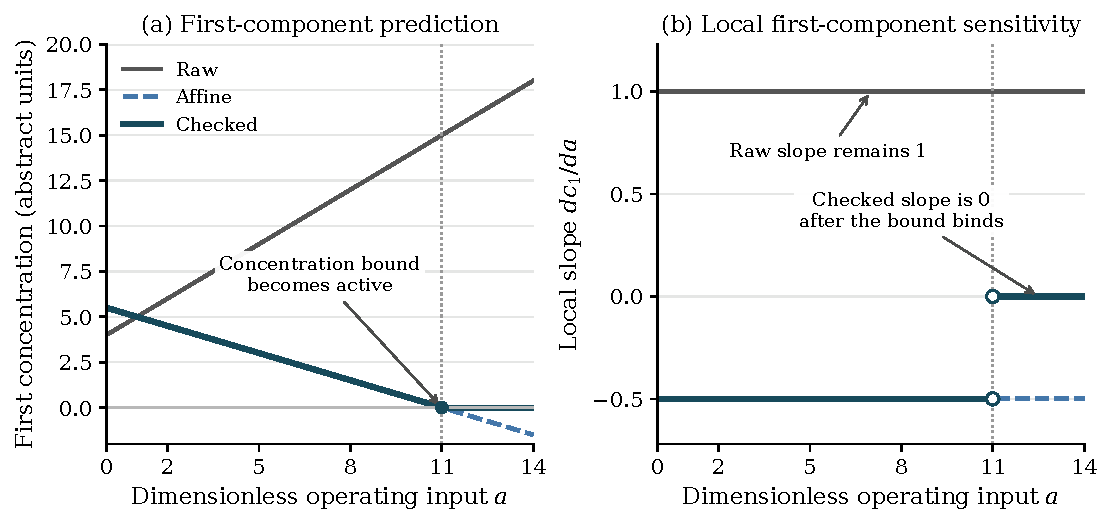
\includegraphics[width=\textwidth]{ch7_concept_branch_sensitivity.pdf}
\caption{Hypothetical first-component response and sensitivity before and after mass conservation and non-negativity enforcement. Open circles mark the two one-sided checked slopes at the active-boundary transition.}
\label{fig:assessment_branch_sensitivity}
\end{figure}

Before the concentration boundary becomes active, the affine and checked responses coincide. Their negative first-component slope differs from the positive raw slope because mass conservation redistributes the operating response across the two components. After the boundary activates, the checked concentration remains at zero and its local slope becomes zero. The transition is therefore characterized by distinct one-sided sensitivities. This example summarizes why interpretation must follow the complete deployed calculation.

\subsection{Assessment design for the structured regression}

\subsubsection{Common inputs and comparator models}

The structured-regression assessment uses a design collection of 10,000 accepted steady-state reactor cases. Every predictor receives the same 22 physical inputs and targets the same 20 effluent components. COD, TN, TP, and TSS are subsequently calculated through the common composition matrix. The input domain, reaction model, simulation bounds, and acceptance criteria remain those of the declared reactor benchmark. The comparison therefore changes the statistical predictor while keeping the physical process and prediction task fixed.

The nine unconstrained comparators are XGBoost, LightGBM, CatBoost, AdaBoost, random forest, support vector regression, \(k\)-nearest neighbors, partial least squares, and a fully connected multilayer perceptron. Together, they represent boosted and randomized tree ensembles, kernel regression, local neighbor averaging, latent linear regression, and nonlinear neural regression. Their methodological foundations include the ensemble construction of \citet{Breiman2001}, the boosting formulations of \citet{Drucker1997}, \citet{ChenGuestrin2016}, \citet{Ke2017}, and \citet{Prokhorenkova2018}, and the latent regression framework of \citet{Wold2001}. These comparators do not use an invariant penalty, auxiliary non-negative fitted-state matrix, or learned component-coupling equation during fitting. The latent components of partial least squares are statistical combinations of the inputs rather than physical process components. The supervised target nevertheless remains the same 20-component effluent state for all methods.

The neural comparator uses hidden layers of 128, 64, and 32 units with logistic activation. Dense connections map the 22 inputs through these layers to the 20 component outputs. Its flexible internal representation is therefore compared with the explicit polynomial structure of ICSOR without changing the prediction target or reporting map.

\subsubsection{Training partitions and hyperparameter selection}

The primary assessment uses a row-wise 80\% training and 20\% held-out split with random seed 42. From the 10,000-case design, 8000 observations form the training pool and 2000 form the final held-out set. Hyperparameter selection uses only the training pool. Half of that pool forms a 4000-row tuning subset, which is further split into 3200 tuning-training and 800 tuning-validation observations.

Each predictor receives 100 hyperparameter trials under a seeded tree-structured Parzen estimator with seed 42. No trial pruning or wall-clock timeout is imposed. \citet{Bergstra2011} develop this search strategy, while \citet{Akiba2019} provide the associated hyperparameter optimization framework. The selection criterion is mean squared error in the shared physical component space on the internal validation set. Once selected, the settings are held fixed for the primary assessment and repeated sample-size study. The final primary model is then fitted using all 8000 training observations.

For the unconstrained comparators, input and output standardization parameters are estimated from the applicable training partition. Predictions are transformed back to physical component coordinates before invariant checking, reporting, or error assessment. ICSOR remains in physical coordinates throughout so that its coefficients, invariant operator, and deployment constraints share the same component convention. Internal-validation transformations are estimated only from the tuning-training rows. Thus, means, standard deviations, and hyperparameters are determined without access to the held-out test responses. Projection weights are likewise fixed before held-out assessment.

Table~\ref{tab:icsor_comparator_settings} lists the specified comparator configurations. These settings describe the fitted models and should not be interpreted as performance results.

\begin{table}[htbp]
\centering\small
\caption{Specified configurations of the nine unconstrained comparators.}\label{tab:icsor_comparator_settings}
\begin{tabular}{p{0.19\textwidth}p{0.74\textwidth}}
\toprule
Comparator & Configuration\\
\midrule
XGBoost & 309 trees, learning rate 0.125, maximum depth 3, minimum child weight 6.84, row fraction 0.915, feature fraction 0.828, absolute penalty \(1.18\times10^{-3}\), and squared penalty 0.382.\\
LightGBM & 302 trees, learning rate 0.0809, 16 leaves, maximum depth 8, minimum leaf count 14, row fraction 0.845, feature fraction 0.869, absolute penalty \(3.17\times10^{-3}\), and squared penalty \(3.36\times10^{-4}\).\\
CatBoost & 236 boosting iterations, learning rate 0.172, depth 4, leaf squared penalty 0.0266, bagging temperature 0.0277, and random strength 0.0657.\\
AdaBoost & 236 estimators, learning rate 0.999, and squared regression loss.\\
Random forest & 390 trees, maximum depth 14, minimum split count 3, minimum leaf count 1, feature fraction 0.500, and no bootstrap resampling.\\
Support vector regression & Polynomial kernel of degree 4, regularization parameter 0.118, insensitive-error width 0.0458, constant offset 0.889, and solver tolerance \(8.96\times10^{-4}\). The kernel scale is the reciprocal of the product of input dimension and training input variance.\\
\(k\)-nearest neighbors & 15 neighbors, inverse-distance weighting, Manhattan distance, and a k-dimensional search tree with leaf size 40.\\
Partial least squares & 6 latent components, maximum 887 fitting iterations, and tolerance \(9.91\times10^{-5}\).\\
Multilayer perceptron & Hidden widths \((128,64,32)\), logistic activation, adaptive moment estimation, squared penalty \(6.33\times10^{-4}\), batch size 64, initial learning rate \(1.08\times10^{-3}\), maximum 500 iterations, and tolerance \(1.63\times10^{-5}\). Training rows are not shuffled, and early stopping is disabled.\\
\bottomrule
\end{tabular}
\end{table}

\subsubsection{Scoring states and physical diagnostics}

The scored ICSOR prediction is its final checked component state. For comparator accuracy assessment, the raw comparator prediction receives the same affine mass-conservation projection in Equation~\eqref{eq:icsor_affine_solution}, after which the common reporting map is applied. The accuracy comparison therefore evaluates the checked structured prediction against comparator predictions aligned to the same invariant equalities. Comparator accuracy scoring uses the affine state, whereas ICSOR accuracy scoring uses the complete deployed state, including the constrained non-negativity projection when required.

The numerical assessment uses an operator \(A_{num}\) obtained by rounding the null-space basis, removing negligible coefficients, and dividing each row by its first nonzero coefficient. Fitting, affine projection, and constrained deployment use this numerical operator in place of the ideal operator \(A\). Reported balance violations therefore refer specifically to these adopted numerical relations and the stated scaling.

Physical diagnostics use the raw comparator predictions rather than their affine-aligned accuracy states. ICSOR diagnostics distinguish the raw coupled prediction, affine projection, and final deployed state. This separation makes it possible to identify which stage produces physical compliance. The empirical balance diagnostic is \(v_{mc}^{num}(c)=\|A_{num}(c-c_{in})\|_2\), while non-negativity is assessed using \(v_{nn}\) from Equation~\eqref{eq:icsor_deployment_diagnostics}. For either diagnostic,
\begin{equation}
\equationname{Percentage frequency of a physical-constraint violation}
\label{eq:icsor_violation_frequency}
f_v=\frac{100}{n}\sum_{i=1}^{n}
\mathbf{1}\{v(c_i)>10^{-10}\}.
\end{equation}
Violation frequencies, residual magnitudes, adjustment distances, and deployment-branch use answer different questions about the same prediction procedure. They are therefore reported alongside, rather than substituted for, predictive error.

\subsubsection{Composite error measures}

The five reported error measures summarize different aspects of predictive disagreement. Consider two hypothetical observations with reference values \((2,4)\) and predictions \((3,2)\). The residuals are \((1,-2)\), their squares are \((1,4)\), and their absolute values are \((1,2)\). The resulting mean squared error is 2.5, root mean squared error is approximately 1.5811, and mean absolute error is 1.5.

The corresponding absolute relative errors are \(1/2\) and \(2/4\), giving a mean relative absolute error of 0.5. The reference mean is 3, with total squared variation \((2-3)^2+(4-3)^2=2\). The prediction residual squared sum is 5, so \(R^2=1-5/2=-1.5\). The negative value indicates that the hypothetical prediction has greater squared error than using the reference mean for both observations. These calculations illustrate why the metrics provide complementary information.

For reported quantity \(q\in\{1,2,3,4\}\), let \(e_{iq}=\widehat y_{iq}-y_{iq}\). The squared, root, and absolute measures are
\begin{equation}
\equationname{Per-composite squared, root, and absolute error measures}
\label{eq:icsor_composite_error_metrics}
E_{2,q}=\frac{1}{n}\sum_i e_{iq}^{2},
\qquad E_{root,q}=\sqrt{E_{2,q}},
\qquad E_{1,q}=\frac{1}{n}\sum_i|e_{iq}|.
\end{equation}
For strictly nonzero reference values,
\begin{equation}
\equationname{Mean relative absolute error of a reported composite}
\label{eq:icsor_relative_error}
E_{rel,q}=\frac{1}{n}\sum_i\frac{|e_{iq}|}{|y_{iq}|}.
\end{equation}
The quantity is reported as a ratio; multiplying by 100 gives a percentage. A zero reference value makes the expression undefined, while a very small reference can make the relative error disproportionately large. Any convention for zero-reference cases must therefore be defined before predictors are compared.

The target-specific coefficient of determination is
\begin{equation}
\equationname{Coefficient of determination for a reported composite}
\label{eq:icsor_coefficient_determination}
R_q^2=1-
\frac{\sum_i e_{iq}^{2}}
{\sum_i(y_{iq}-\overline y_q)^2}.
\end{equation}
A target with no reference variation makes the expression undefined. Negative values are possible when the prediction error exceeds that of the reference-mean predictor.

The aggregate root error pools residuals across the four reported quantities:
\begin{equation}
\equationname{Root mean squared error pooled across four reported composites}
\label{eq:icsor_aggregate_root_error}
E_{root}=\left(\frac{1}{4n}\sum_{q=1}^{4}\sum_{i=1}^{n}e_{iq}^{2}\right)^{1/2}.
\end{equation}
Aggregate absolute and relative errors use the corresponding means across observations and reported quantities, while aggregate \(R^2\) is the mean of the four target-specific coefficients. Because the composite coordinates retain their own physical units, the pooled error is a benchmark summary under that numerical convention rather than a dimensionless measure. Per-target scores remain necessary to identify which reported quantities drive the aggregate.

Pooling before taking the square root is also distinct from averaging target-specific root errors. If four hypothetical target mean squared errors are 1, 9, 1, and 9, the pooled mean squared error is 5 and the pooled root error is \(\sqrt5\approx2.2361\). The average of the four target root errors is instead \((1+3+1+3)/4=2\). Equation~\eqref{eq:icsor_aggregate_root_error} defines the first of these two summaries.

The primary ordering measure is aggregate root mean squared error. The remaining measures provide complementary perspectives: squared error emphasizes large residuals, absolute error describes average deviation, relative error scales that deviation to the reference magnitude, and \(R^2\) relates squared error to target variation. Predictor rankings are therefore examined separately under each measure.

\subsubsection{Repeated sample-size assessment}

The sample-size assessment uses
\begin{equation}
\equationname{Observation counts for structured-regression sample-size assessment}
\label{eq:icsor_assessment_sizes}
n\in\{500,1450,2400,3350,4300,5250,6200,7150,8100,9050,10000\}.
\end{equation}
At each size, ten subsamples are drawn without replacement from the design collection using deterministic seeds derived from 42. Each subsample receives an 80\% training and 20\% held-out split, and all ten predictors use the same sampled rows and partitions. The complete design therefore contains 110 fits per predictor.

The selected hyperparameters remain fixed across this assessment. This isolates the effect of data availability under a common model specification rather than allowing each sample size to define a new tuned model. Mean held-out scores and their variability are summarized across the ten runs. These learning curves show how the relative value of model flexibility and structural constraints changes with the simulation budget \citep{Geman1992,VieringLoog2023}.

The learning-curve area can be understood from a reduced example. Suppose an error measure takes values 6, 4, and 3 at sample sizes 100, 200, and 400. The first trapezoid has width 100 and average height 5, giving area 500. The second has width 200 and average height 3.5, giving area 700. The total area is therefore 1200. Dividing by the complete width \(400-100=300\) gives a normalized area of 4. Wider sample-size intervals contribute proportionally more to this average.

For retained sizes \(n_1,\ldots,n_S\), the numerical approximation is
\begin{equation}
\equationname{Trapezoidal approximation of normalized learning-curve area}
\label{eq:icsor_learning_area_trapezoids}
\frac{1}{n_{max}-n_{min}}
\sum_{s=1}^{S-1}(n_{s+1}-n_s)
\frac{\overline M_{m,j}(n_s)+\overline M_{m,j}(n_{s+1})}{2}.
\end{equation}
The corresponding continuous definition is
\begin{equation}
\equationname{Integral definition of normalized learning-curve area}
\label{eq:icsor_learning_area}
L_{m,j}=\frac{1}{n_{max}-n_{min}}
\int_{n_{min}}^{n_{max}}\overline M_{m,j}(n)\,\mathrm{d}n.
\end{equation}
Here \(\overline M_{m,j}(n)\) is the mean held-out value of measure \(j\) for predictor \(m\) at sample size \(n\). Dividing by the sample-size interval makes the result an average curve height and preserves the units of the original measure. \citet{Cawley2011} and \citet{Guyon2011} provide related trajectory summaries in active learning, while the present study varies the number of randomly sampled training observations.

Ranks provide a separate view of relative ordering. If four hypothetical errors are 3.0, 3.0, 4.5, and 6.0, their dense ranks are 1, 1, 2, and 3. The tie receives the same rank, and the next distinct score receives the next consecutive rank. The numerical distance between 4.5 and 6.0 does not affect the difference between their ranks.

For each measure \(j\), reported quantity \(q\), and retained sample size \(n_s\), predictors receive a dense rank \(r_{m,j,q}(n_s)\) based on their mean held-out score. Lower squared, root, absolute, and relative errors receive better ranks, whereas larger \(R^2\) values receive better ranks. With \(S=11\) sizes and five measures,
\begin{equation}
\equationname{Mean dense ranks over quantities, measures, and sample sizes}
\label{eq:icsor_dense_rank}
\overline r_{m,j}=\frac{1}{4S}\sum_{q=1}^{4}\sum_{s=1}^{S}r_{m,j,q}(n_s),
\qquad
\overline r_m=\frac{1}{5}\sum_{j=1}^{5}\overline r_{m,j}.
\end{equation}
These summaries describe relative performance over the declared comparisons. \citet{Demsar2006} develops broader rank-based model comparisons, while \citet{Shevchenko2024} emphasize the importance of benchmarking variability. Absolute error and mean rank are therefore reported together so that ordering is not detached from error magnitude.

At the largest sample size, the generalization gap is
\begin{equation}
\equationname{Held-out minus training root-error gap}
\label{eq:icsor_generalization_gap}
\Delta E_{root,m}=E_{root,m}^{held\text{-}out}-E_{root,m}^{training}.
\end{equation}
A positive value indicates greater held-out error. The gap does not by itself measure predictive quality: a model can have a small gap because it performs similarly well on training and held-out data, or because it performs similarly poorly on both. For example, training and held-out errors of 0.5 and 0.8 give a gap of 0.3, while errors of 5.0 and 5.1 give a smaller gap of 0.1 despite much worse prediction. The gap is therefore interpreted together with the absolute error \citep{Hastie2009}.

Training time is recorded for every repeated fit and summarized across runs. Deployment effort is assessed separately through prediction time, branch use, and constrained-solve effort. This separation distinguishes the cost of constructing the approximation from the cost of returning a physically checked state.

\subsection{Interpretability assessment}

The interpretability assessment examines the six driver blocks, the coupling matrix, and the corresponding raw component and composite mappings. It asks what the fitted structure reveals about the response within the declared process domain. \citet{Brunton2016} connect interpretable nonlinear terms to the broader problem of recovering mathematical structure from data, while \citet{Machado2014} show how operational and influent uncertainty complicate interpretation in activated sludge systems.

The driver and coupling parameters can trade off in the simultaneous relation \(Rc=B\phi\). Different joint stationary solutions can therefore produce similar component predictions using different coefficient allocations \citep{Selerio2026}. The imposed symmetry removes one source of redundancy in the ordered quadratic terms, but it does not establish unique causal parameter identification. Coefficient signs and magnitudes are therefore interpreted together with the complete fitted response rather than in isolation.

Prediction error and physical diagnostics are also separated across the raw regression, affine projection, and final deployed state. This distinction makes clear what the statistical model learns and what the projection subsequently imposes \citep{Karniadakis2021,KircherVotsmeier2025}. Projection magnitude is examined because a final state can satisfy the adopted constraints while remaining far from the raw prediction. Likewise, fitting effort and deployment effort are recorded separately because they represent different computational costs.

The assessment is therefore limited to steady-state component prediction within the stated input domain and control volume. The raw regression provides an inspectable statistical approximation. Checked deployment then imposes the adopted numerical invariants and non-negativity requirements on the returned state.

\section{Results}
\label{sec:icsor_results}

\subsection{Accuracy on the fixed held-out partition}

Table~\ref{tab:icsor_fixed_results} summarizes predictive performance on the 2000 fixed held-out cases. ICSOR is evaluated using its final checked state, while the comparator predictions are evaluated after affine alignment to the adopted mass conservation relations. The multilayer perceptron produced the lowest pooled root mean squared error at 4.38, followed by LightGBM at 5.30. Support vector regression and ICSOR were closely spaced at 5.97 and 5.98, respectively. Under the pooled native composite-coordinate convention of Equation~\eqref{eq:icsor_aggregate_root_error}, ICSOR therefore provided competitive but not leading full-data accuracy.

\begin{table}[htbp]
\centering\small
\caption{Fixed-split held-out composite performance. ICSOR is scored after checked deployment. Comparators are scored after affine alignment without a non-negativity constraint. Relative absolute error is a ratio rather than a percentage.}
\label{tab:icsor_fixed_results}
\begin{tabular}{p{4.7cm}rrrr}
\toprule
Predictor & $E_{root}$ & $E_1$ & Mean $R^2$ & $E_{rel}$\\
\midrule
Multilayer perceptron & 4.38 & 2.55 & 0.9915 & 0.0123\\
LightGBM & 5.30 & 3.21 & 0.9806 & 0.0203\\
Support vector regression & 5.97 & 3.49 & 0.9713 & 0.0244\\
ICSOR & 5.98 & 3.70 & 0.9700 & 0.0256\\
XGBoost & 6.12 & 3.81 & 0.9733 & 0.0244\\
CatBoost & 6.45 & 4.07 & 0.9727 & 0.0250\\
AdaBoost & 21.27 & 13.15 & 0.8643 & 0.0653\\
$k$-nearest neighbors & 23.61 & 13.87 & 0.8535 & 0.0557\\
Partial least squares & 28.24 & 17.05 & 0.7808 & 0.0681\\
Random Forest & 29.00 & 16.93 & 0.7934 & 0.0632\\
\bottomrule
\end{tabular}
\end{table}

Relative to the two leading predictors, ICSOR's pooled root error was 36.5\% higher than that of the multilayer perceptron and 12.8\% higher than that of LightGBM. It nevertheless remained slightly below XGBoost and CatBoost on the same measure. Its mean absolute relative error of 0.0256 corresponds to 2.56\%. The fixed-split comparison therefore quantifies the predictive cost associated with using the more structured model under the largest-data setting.

Figure~\ref{fig:icsor_fixed_results} shows the same comparison for pooled root error, pooled absolute error, and mean composite \(R^2\). ICSOR ranked fourth by pooled root error on this partition, reinforcing the conclusion that its principal advantage at the largest design size is not minimum error alone.

\begin{figure}[htbp]
\centering
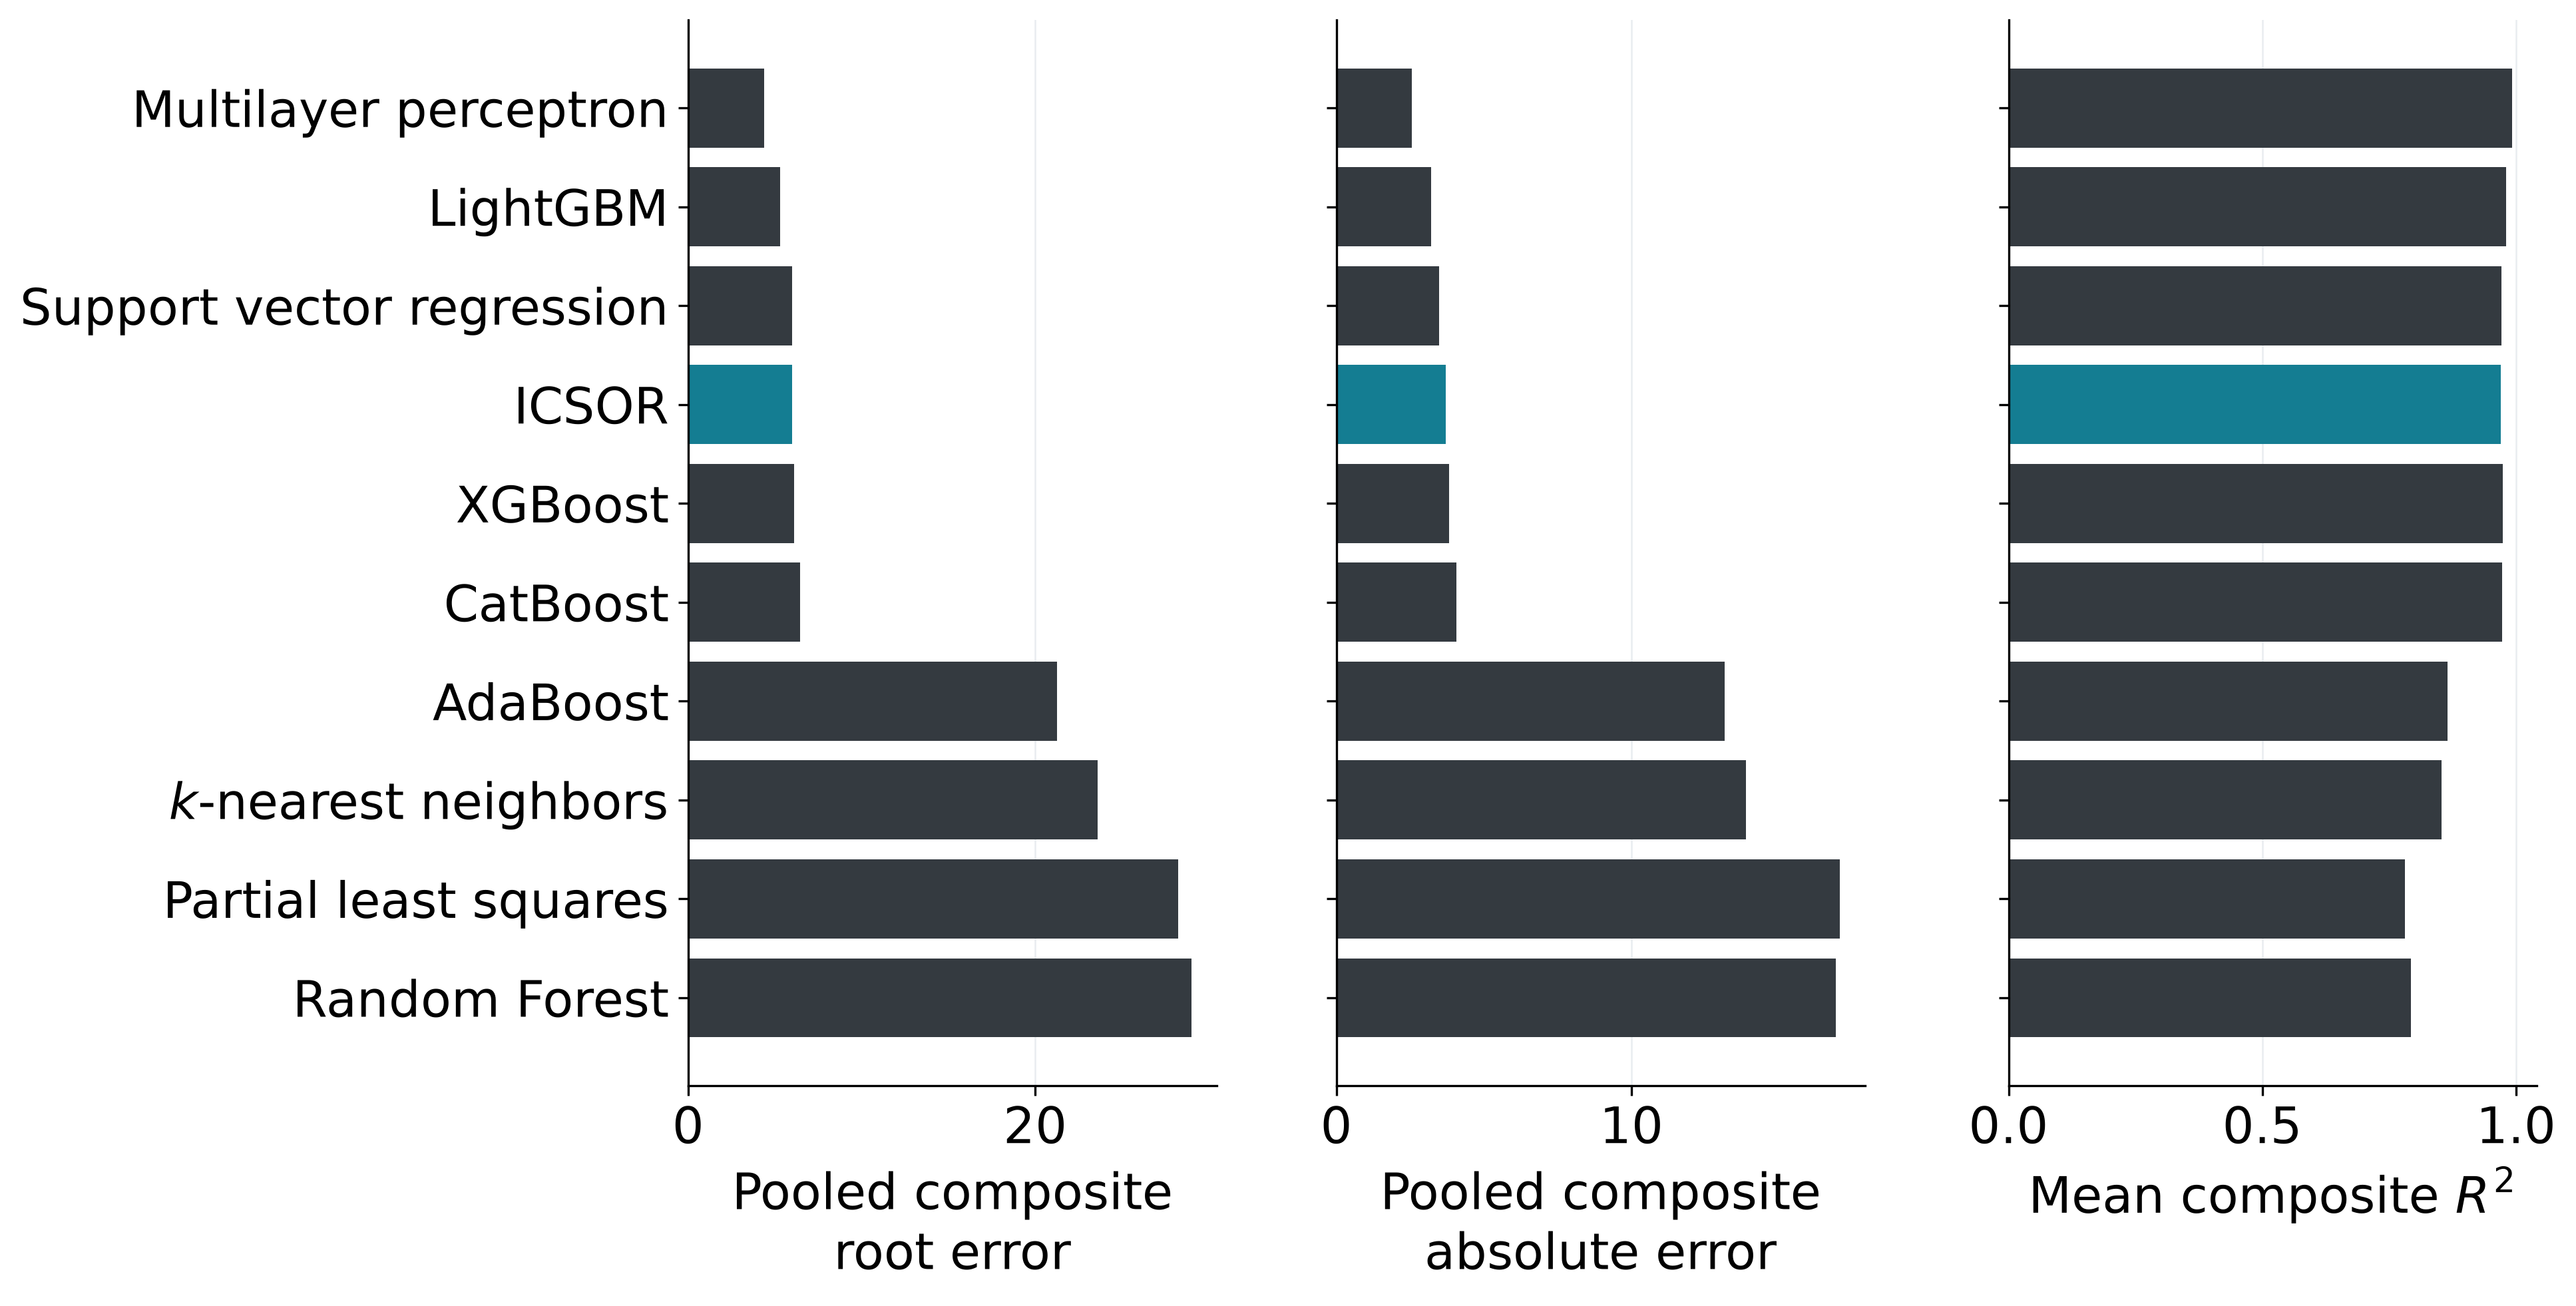
\includegraphics[width=\textwidth]{results/ch5/q01_fixed_split_accuracy.png}
\caption{Fixed-split composite accuracy on 2000 held-out cases. Teal bars identify ICSOR after checked deployment. Gray bars identify comparators after affine alignment. Pooled root and absolute errors retain the native composite-coordinate convention. The right panel averages four composite-specific $R^2$ values.}
\label{fig:icsor_fixed_results}
\end{figure}

The aggregate score also hides differences among the individual treatment quantities. Table~\ref{tab:icsor_target_results} separates COD, TN, TP, and TSS. ICSOR's COD root error was 7.77, only 0.18 above LightGBM and lower than that of the other non-neural predictors. Its TN and TSS errors were 3.55 and 8.36, respectively. The multilayer perceptron produced the lowest COD, TN, and TSS errors. All methods had the same TP error of 0.0361 after the specified alignment and reporting procedure, so TP did not distinguish the predictors in this comparison.

\begin{table}[htbp]
\centering\small
\caption{Fixed-split root mean squared error for each composite. COD, TN, TP, and TSS use g COD m$^{-3}$, g N m$^{-3}$, g P m$^{-3}$, and g TSS m$^{-3}$, respectively.}
\label{tab:icsor_target_results}
\begin{tabular}{p{4.7cm}rrrr}
\toprule
Predictor & COD & TN & TP & TSS\\
\midrule
Multilayer perceptron & 6.48 & 1.58 & 0.0361 & 5.66\\
LightGBM & 7.59 & 2.77 & 0.0361 & 6.85\\
Support vector regression & 8.87 & 3.50 & 0.0361 & 7.20\\
ICSOR & 7.77 & 3.55 & 0.0361 & 8.36\\
XGBoost & 8.78 & 3.27 & 0.0361 & 7.88\\
CatBoost & 9.13 & 3.23 & 0.0361 & 8.53\\
AdaBoost & 38.30 & 5.58 & 0.0361 & 17.68\\
$k$-nearest neighbors & 38.24 & 4.23 & 0.0361 & 27.37\\
Partial least squares & 43.22 & 5.09 & 0.0361 & 36.00\\
Random Forest & 45.87 & 4.00 & 0.0361 & 35.26\\
\bottomrule
\end{tabular}
\end{table}

Figure~\ref{fig:icsor_composite_results} makes the scale difference among these quantities visible. COD and TSS contributed much larger numerical errors to the pooled score than TP. The separate target panels are therefore necessary for interpreting what the aggregate comparison represents.

\begin{figure}[htbp]
\centering
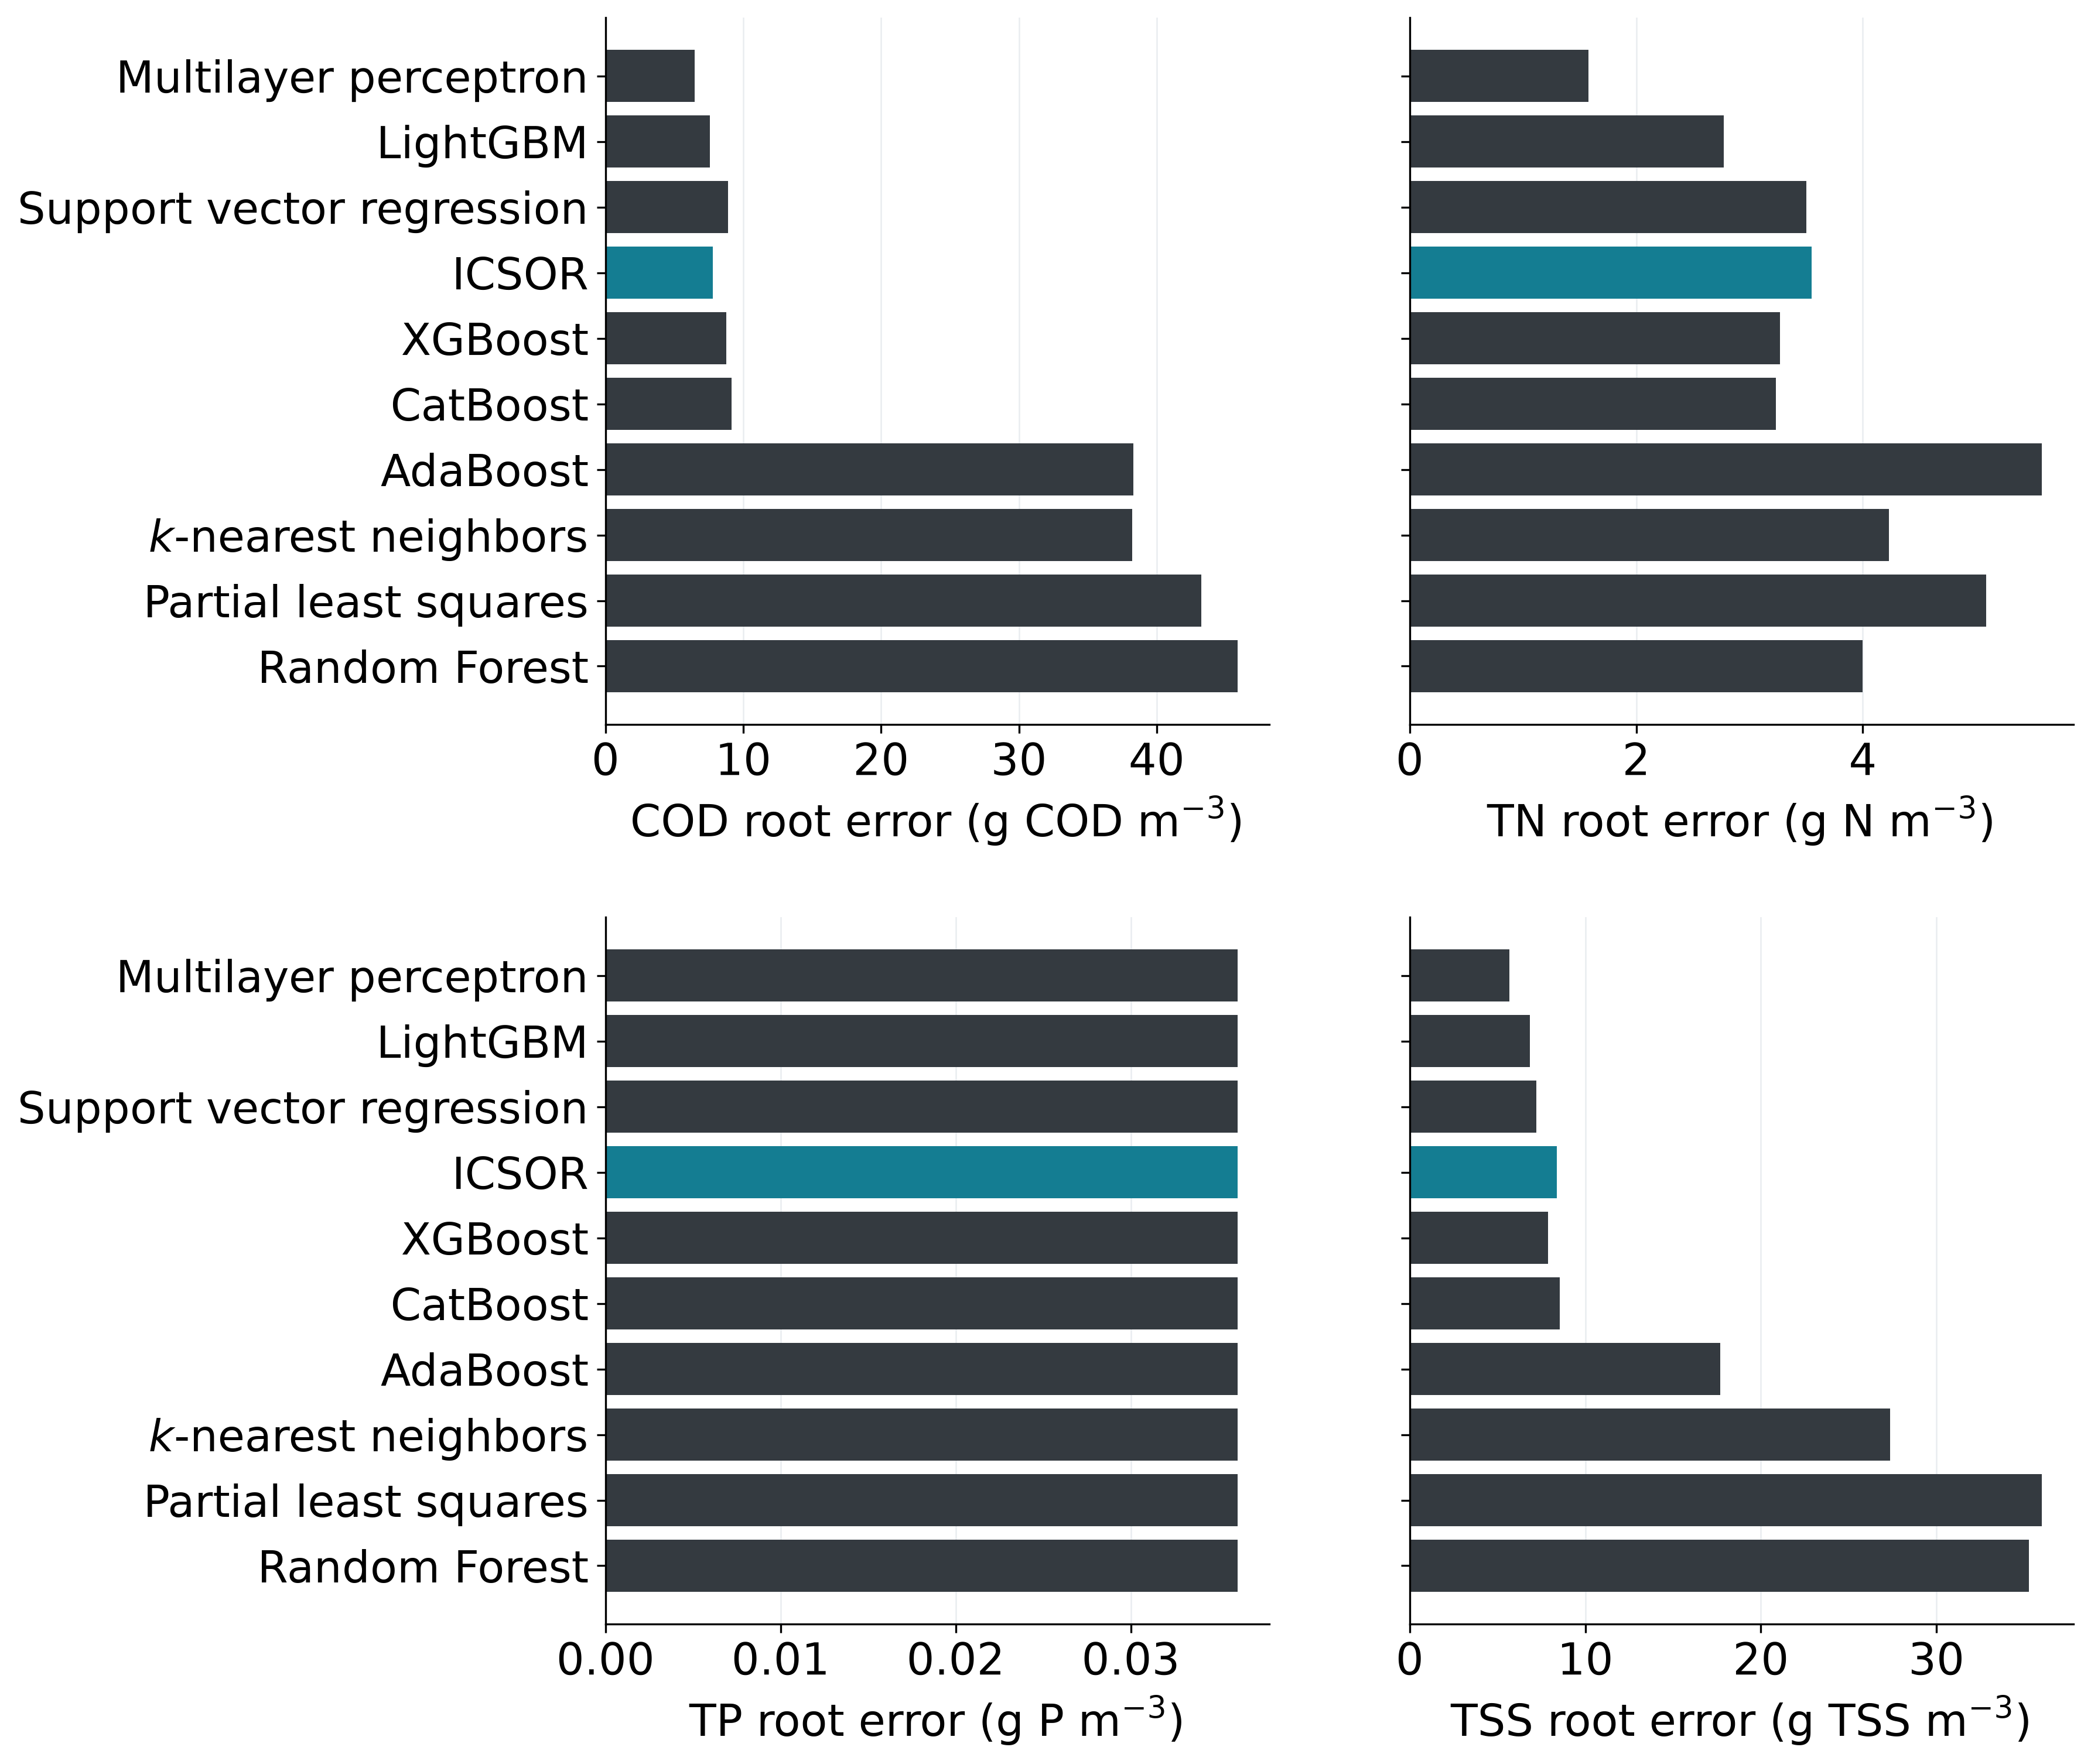
\includegraphics[width=\textwidth]{results/ch5/q02_composite_accuracy.png}
\caption{Fixed-split root mean squared error for COD, TN, TP, and TSS. Teal identifies ICSOR and gray identifies the comparators. Each panel has its own constituent unit and horizontal scale. All methods have the same reported TP error under the specified alignment and reporting procedure.}
\label{fig:icsor_composite_results}
\end{figure}

\subsection{Sample efficiency and generalization}

The repeated sample-size assessment produced a different picture from the fixed large-data comparison. At the smallest design size of 500 cases, ICSOR had the lowest mean held-out root error at 10.79. XGBoost and LightGBM followed at 11.26 and 11.45, while the multilayer perceptron ranked fifth at 13.26. At the largest design size, however, the ordering changed: the multilayer perceptron reached 4.62, LightGBM 5.27, support vector regression 5.84, and ICSOR 5.94. The leading model therefore depended on the available simulation budget rather than remaining fixed across the learning curve.

\begin{table}[htbp]
\centering\small
\caption{Repeated-split composite assessment over eleven design sizes and ten runs per size. Final error and the held-out minus training gap refer to $n=10{,}000$. The learning-curve area is normalized by the design-size interval. Lower error and curve-area values indicate better performance. The gap measures the separation between training and held-out error.}
\label{tab:icsor_scaling_results}
\begin{tabular}{p{4.3cm}rrrr}
\toprule
Predictor & \begin{tabular}{r}Final\\$E_{root}$\end{tabular} & \begin{tabular}{r}Normalized\\curve area\end{tabular} & Mean rank & $\Delta E_{root}$\\
\midrule
Multilayer perceptron & 4.62 & 6.75 & 2.5 & 0.65\\
LightGBM & 5.27 & 6.35 & 2.2 & 1.99\\
Support vector regression & 5.84 & 6.90 & 4.0 & 1.19\\
ICSOR & 5.94 & 6.33 & 4.3 & 0.22\\
XGBoost & 6.10 & 7.01 & 4.3 & 1.44\\
CatBoost & 6.26 & 7.60 & 5.0 & 0.69\\
AdaBoost & 21.42 & 20.29 & 8.2 & 0.23\\
$k$-nearest neighbors & 23.76 & 25.77 & 7.0 & 23.66\\
Partial least squares & 27.96 & 30.17 & 9.4 & 0.38\\
Random Forest & 28.78 & 30.31 & 8.2 & 18.71\\
\bottomrule
\end{tabular}
\end{table}

Across the complete range of design sizes, ICSOR had the lowest normalized root-error curve area at 6.33. LightGBM was nearly identical at 6.35 and achieved the best mean dense rank of 2.2. The multilayer perceptron had the second-best mean rank at 2.5, while ICSOR and XGBoost both had a mean rank of 4.3. These summaries emphasize different aspects of performance: the curve area favors sustained low root error across the data range, whereas the rank aggregates relative ordering across targets, metrics, and sizes. ICSOR therefore led one trajectory summary without leading all comparative summaries.

Its training-to-held-out behavior also differed from that of the more flexible learners. At the largest design size, ICSOR's held-out minus training root-error gap was 0.22, smaller than the corresponding gaps for the multilayer perceptron, LightGBM, XGBoost, and support vector regression. Partial least squares also had a small gap of 0.38, but its held-out root error was 27.96. A small gap alone therefore did not imply useful prediction. ICSOR combined a small gap with substantially lower absolute error than partial least squares, while the most accurate flexible learners still achieved lower final prediction error.

Figure~\ref{fig:icsor_efficiency_results} separates the normalized curve area, mean dense rank, and final generalization gap. The figure reinforces that no single summary dominates the interpretation: ICSOR led the root-error area, LightGBM led the mean-rank comparison, and the absolute held-out error remained necessary for interpreting the generalization gap.

\begin{figure}[htbp]
\centering
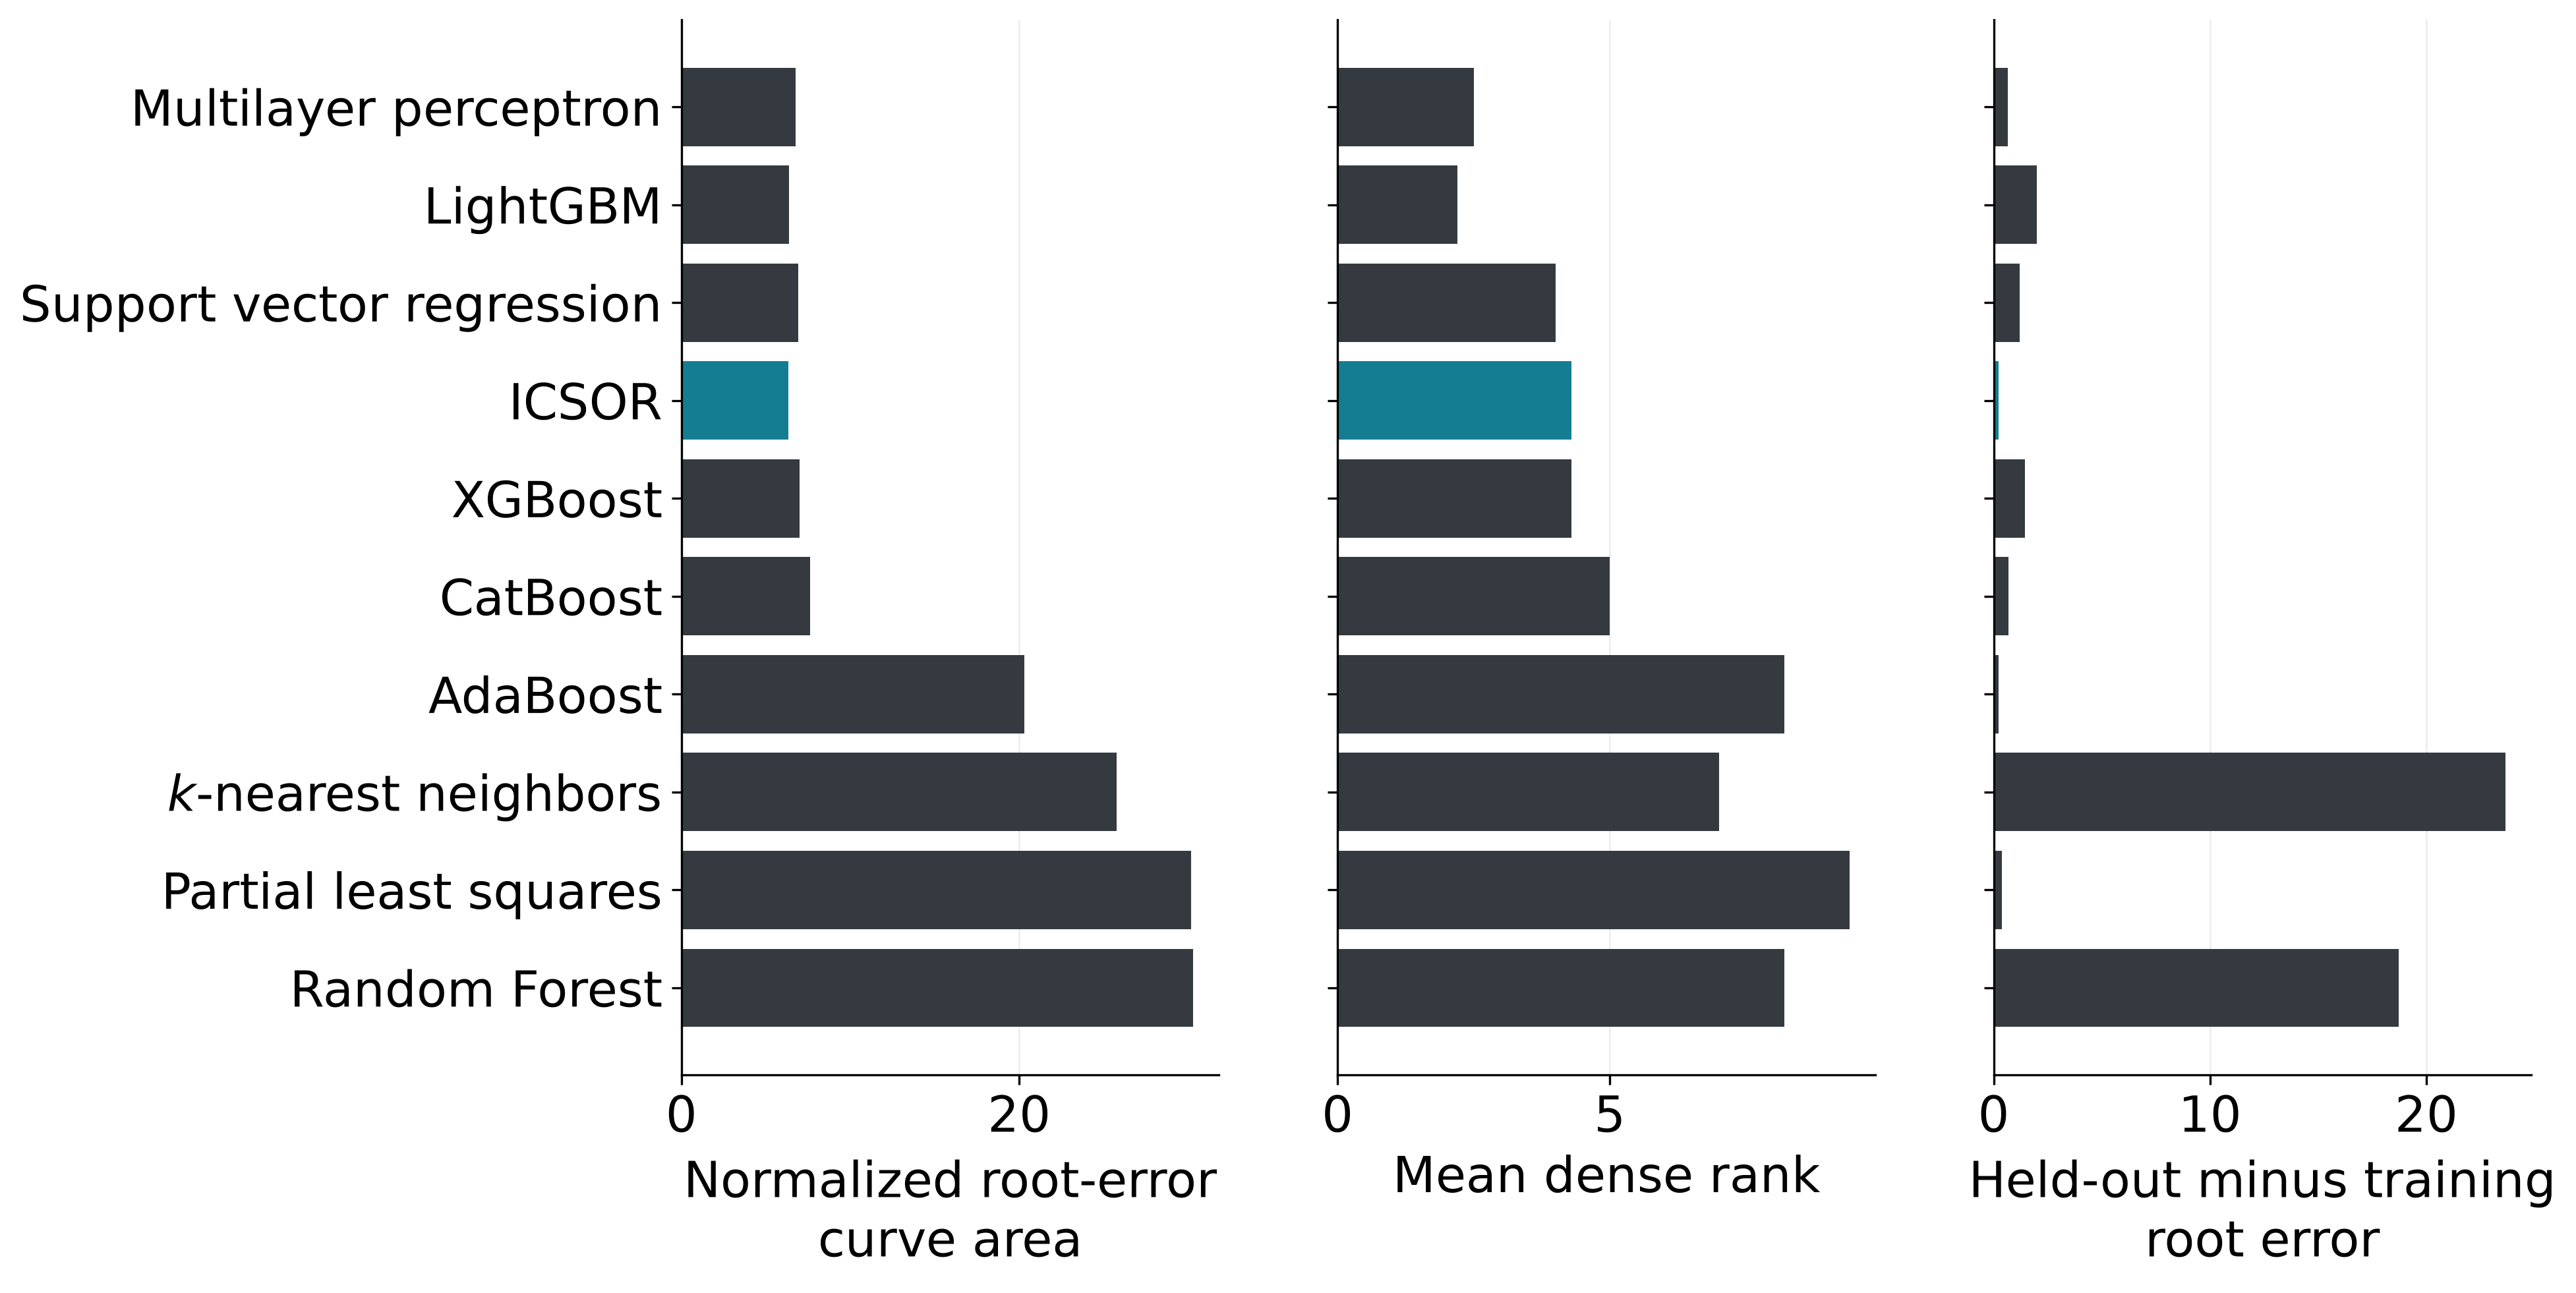
\includegraphics[width=\textwidth]{results/ch5/q03_sample_efficiency.png}
\caption{Normalized root-error curve area, mean dense rank, and held-out minus training root-error gap. Curve areas and ranks summarize eleven design sizes with ten repeated splits per size. The gap refers to the largest design size. Teal identifies ICSOR. The gap is reported alongside the held-out error.}
\label{fig:icsor_efficiency_results}
\end{figure}

The change in model ordering is especially clear at the two endpoints shown in Figure~\ref{fig:icsor_budget_results}. ICSOR led the four selected predictors when only 500 cases were available, whereas the multilayer perceptron had the lowest error at 10,000 cases. The result therefore supports a conditional interpretation of the structured model: its advantage is strongest when simulation data are limited, while flexible nonlinear learners benefit more from the larger design.

\begin{figure}[htbp]
\centering
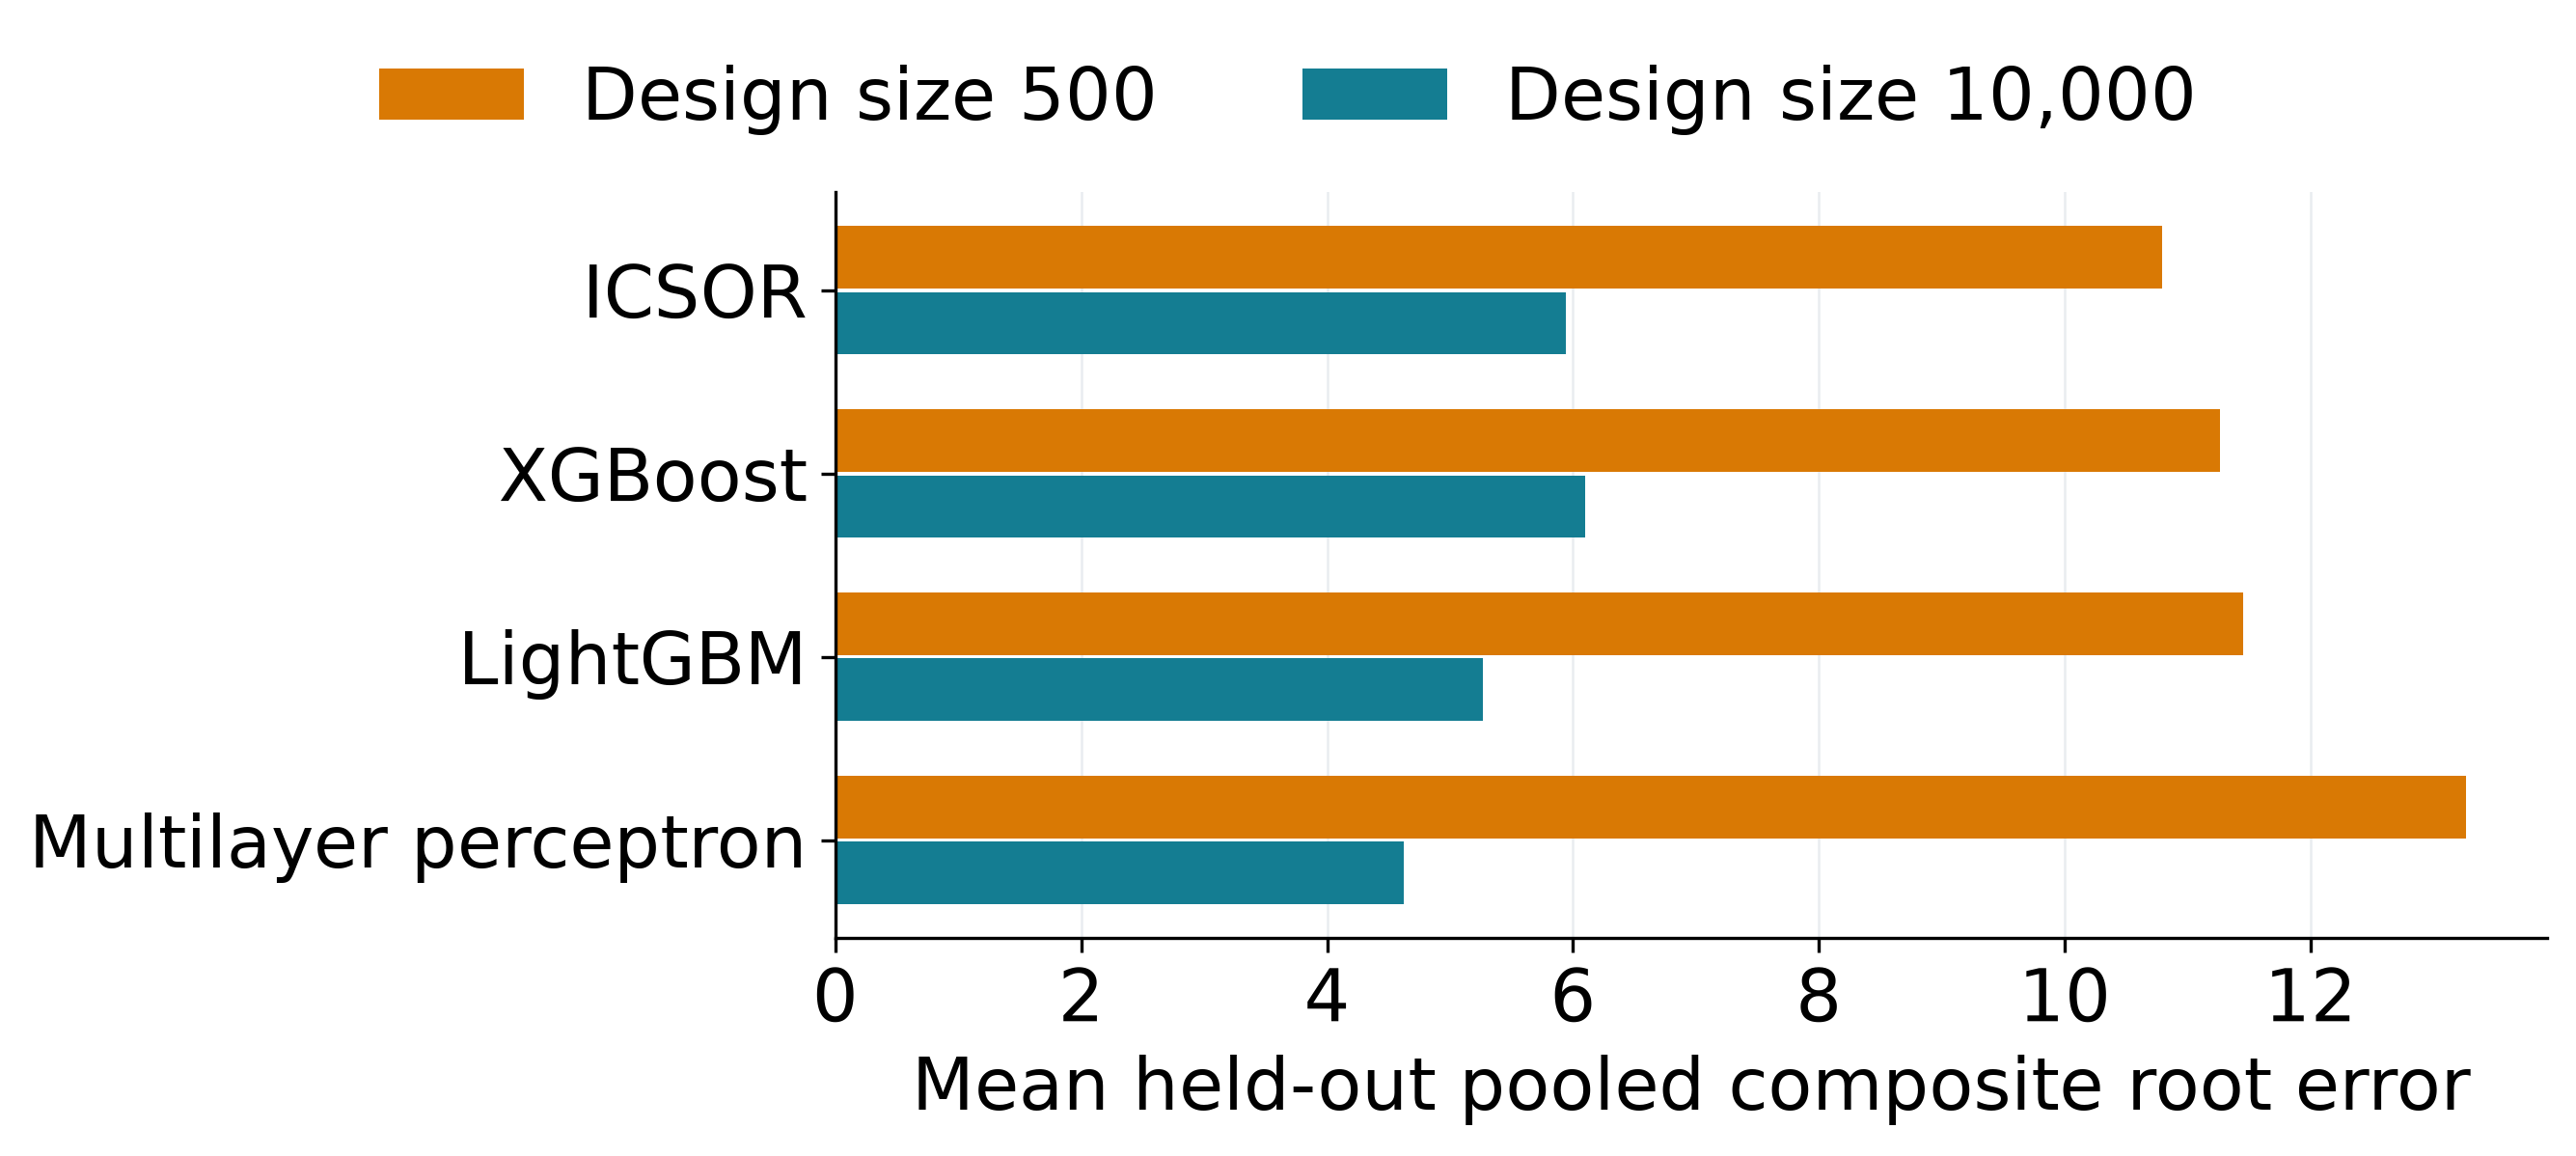
\includegraphics[width=\textwidth]{results/ch5/q04_data_budget_comparison.png}
\caption{Mean held-out pooled composite root error at design sizes 500 and 10,000 for ICSOR, XGBoost, LightGBM, and the multilayer perceptron. Values summarize ten repeated splits. The panels show repeated-split endpoint means at the two specified design sizes.}
\label{fig:icsor_budget_results}
\end{figure}

\subsection{Physical checks and deployment branches}

The physical diagnostics distinguish statistical prediction from the properties of the returned component state. Table~\ref{tab:icsor_physical_results} compares the final ICSOR output with the raw outputs of the nine comparators. Every final ICSOR state satisfied both the adopted numerical balances and non-negativity tolerance. By contrast, every raw comparator state violated the adopted balance tolerance. Several comparators---AdaBoost, random forest, and \(k\)-nearest neighbors---produced no negative raw states, but this did not make them mass conserving. For the remaining comparators, raw non-negativity violation rates ranged from 46.00\% to 70.10\%.

\begin{table}[htbp]
\centering\small
\caption{Component-state violation frequencies on the 2000 held-out cases. ICSOR uses its final checked state. Comparators use their raw state, not the affine-aligned state used for accuracy scoring. Balance violations refer to $A_{num}$ and the declared $10^{-10}$ tolerance.}
\label{tab:icsor_physical_results}
\begin{tabular}{p{5.2cm}rr}
\toprule
Predictor & Balance violations (\%) & Negative states (\%)\\
\midrule
Multilayer perceptron & 100.0 & 58.20\\
LightGBM & 100.0 & 46.00\\
Support vector regression & 100.0 & 68.65\\
ICSOR & 0.0 & 0.00\\
XGBoost & 100.0 & 64.95\\
CatBoost & 100.0 & 70.10\\
AdaBoost & 100.0 & 0.00\\
$k$-nearest neighbors & 100.0 & 0.00\\
Partial least squares & 100.0 & 48.70\\
Random Forest & 100.0 & 0.00\\
\bottomrule
\end{tabular}
\end{table}

The stage-wise ICSOR diagnostics show how this final compliance was obtained. None of the raw coupled predictions passed both physical checks because all violated the adopted balance tolerance, although 21.7\% were already non-negative. Affine projection restored the balance equalities in every case and simultaneously produced a non-negative state for 436 predictions, or 21.8\% of the held-out set. These states could be returned immediately. The remaining 1564 cases, or 78.2\%, required the weighted linear projection to enforce non-negativity while preserving the balances. That solve required a mean of 23.5 iterations and a maximum of 40. Every resulting final state passed both checks.

Figure~\ref{fig:icsor_deployment_results} separates the raw comparator diagnostics from the internal stages of ICSOR deployment. This separation is essential because the final zero-violation result was not a property of the raw regression. It was produced by the projection procedure. The affine stage supplied balance compliance, while the constrained linear projection supplied the additional correction needed for most cases to satisfy non-negativity.

\begin{figure}[htbp]
\centering
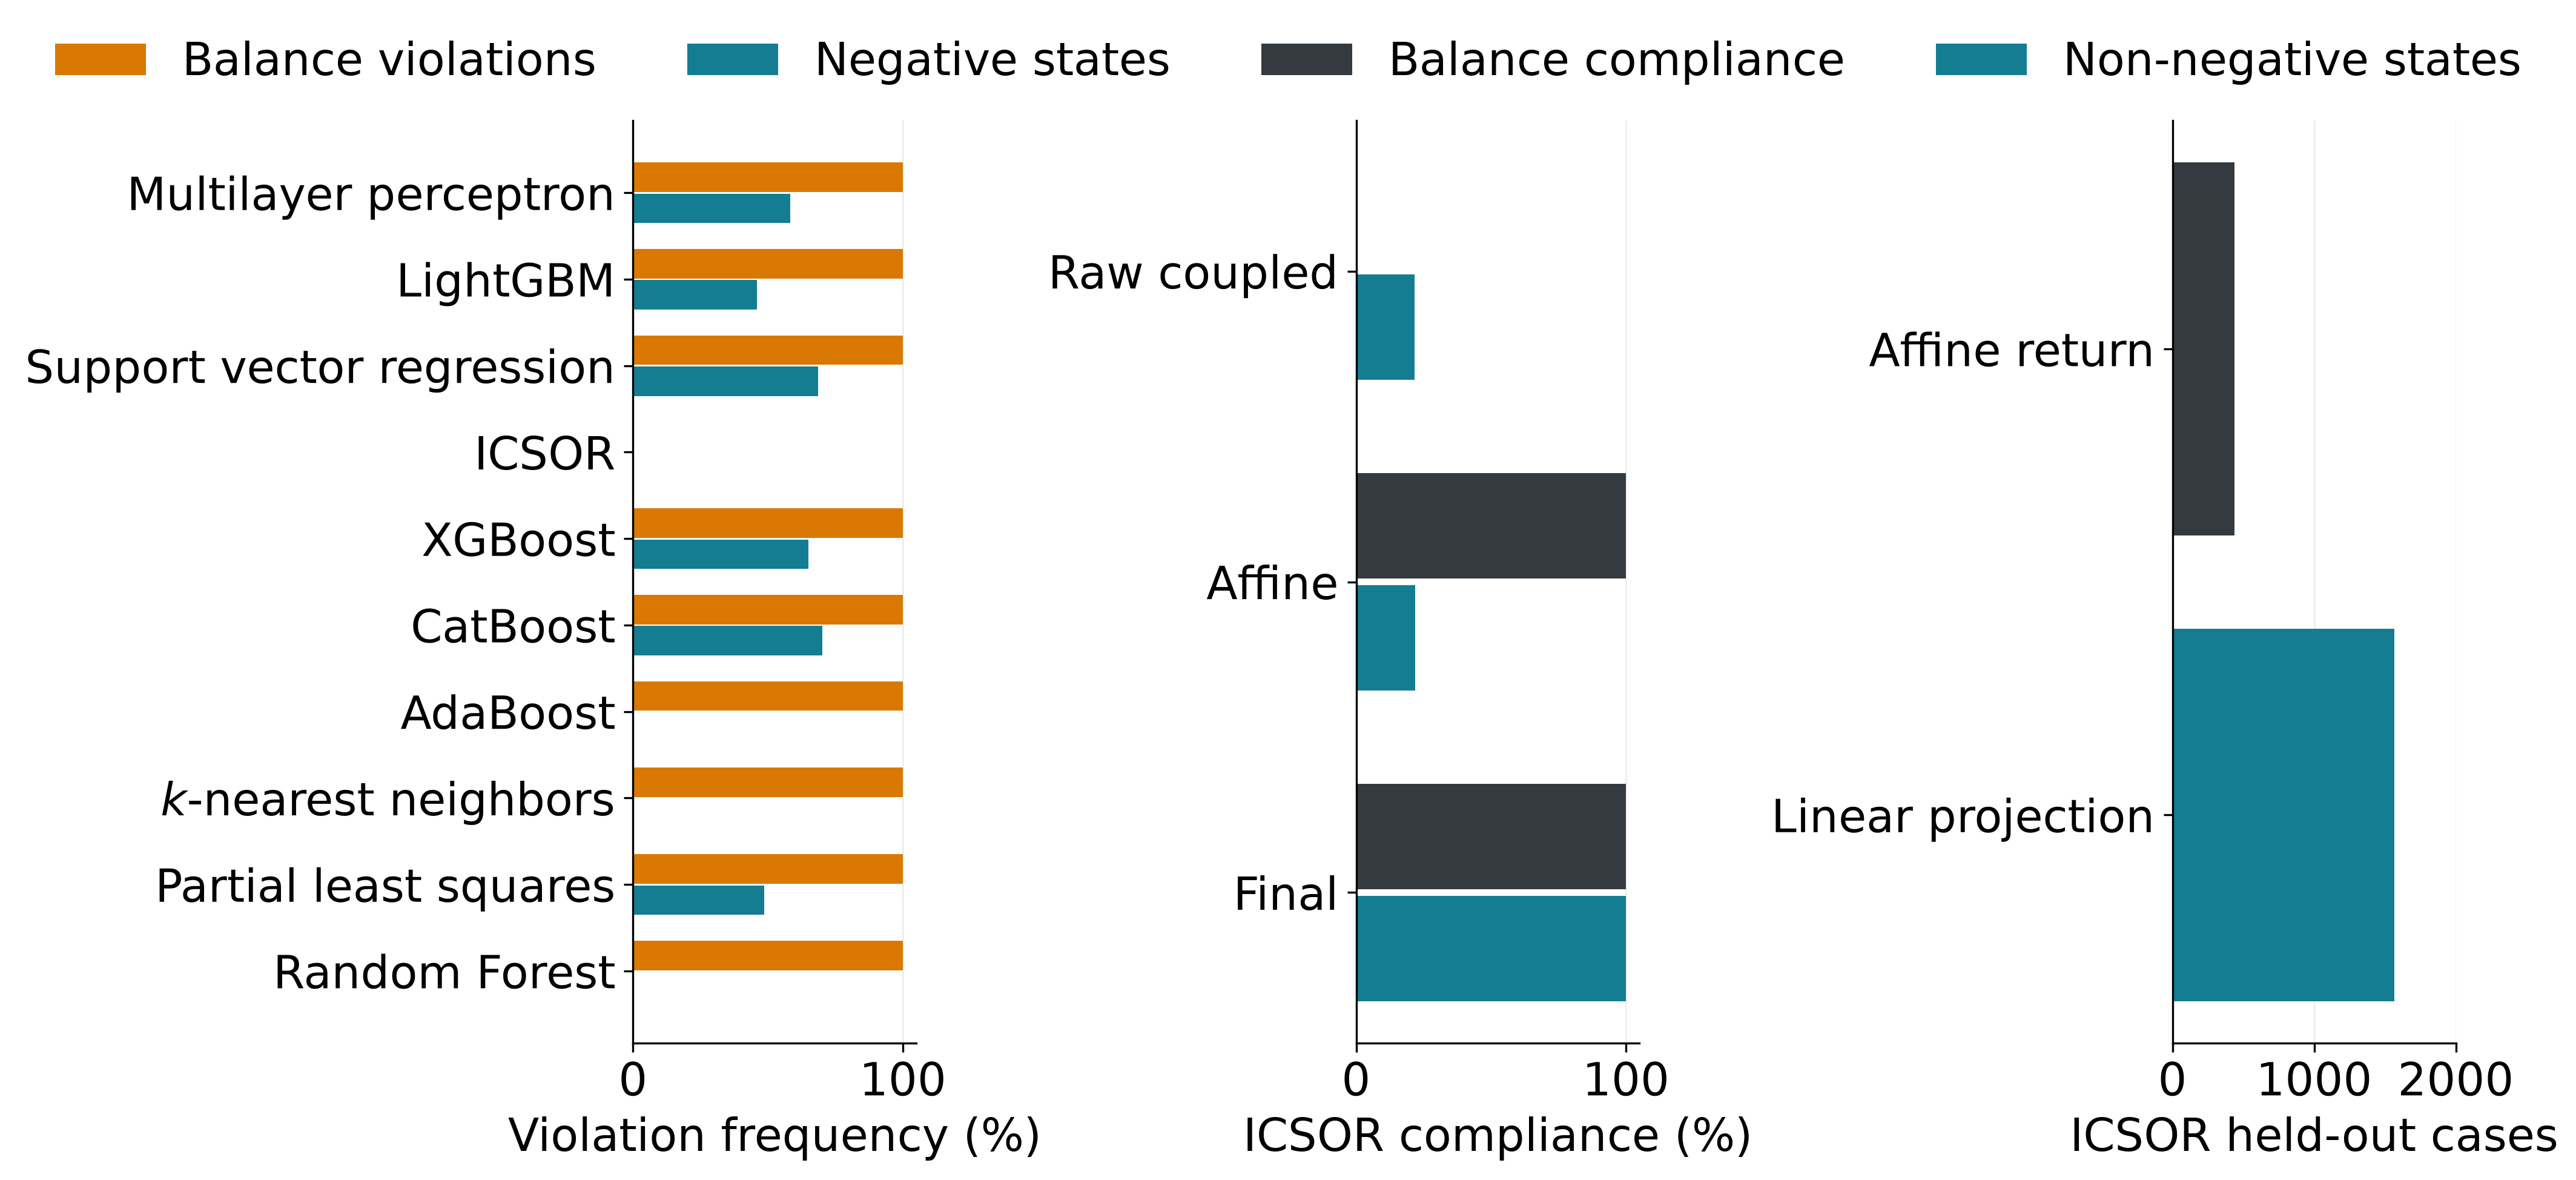
\includegraphics[width=\textwidth]{results/ch5/q05_physical_deployment.png}
\caption{Physical diagnostics and ICSOR deployment on 2000 held-out cases. The left panel compares final ICSOR states with raw comparator states. The middle panel separates raw coupled, affine, and final ICSOR compliance. The right panel gives the numbers returned after affine projection and after constrained linear projection. Balance checks use the adopted numerical operator $A_{num}$.}
\label{fig:icsor_deployment_results}
\end{figure}

The branch counts therefore identify the source of physical admissibility. Fitting guidance alone did not make the raw state compliant. The affine projection restored the adopted invariant relations, and the constrained projection handled the remaining concentration violations. The complete checked deployment procedure, rather than the regression by itself, produced the zero final violation rates.

\subsection{Computational effort}

The structured fitting procedure required more computation than the fastest comparators, but its relative cost changed with the design size. At 500 cases, mean ICSOR fitting time was 21.5 s, compared with 4.72 s for LightGBM, 3.16 s for XGBoost, and 4.99 s for the multilayer perceptron. At 10,000 cases, ICSOR required 94.4 s. LightGBM and the other fast tree ensembles remained much faster, while partial least squares and \(k\)-nearest neighbors required only 0.228 and 2.70 s, respectively.

ICSOR was nevertheless not the slowest model at the largest design size. Its mean fitting time remained below AdaBoost at 117.7 s, support vector regression at 136.8 s, and the multilayer perceptron at 161.6 s. The result places the structured fit between the fastest conventional regressors and several computationally heavier nonlinear alternatives.

Fitting time is only one part of the computational requirement. Most fixed-split ICSOR predictions also required constrained deployment: the linear projection branch was activated in 78.2\% of cases. The reported iteration counts therefore represent additional repeated-use effort beyond the raw regression evaluation. Separating fitting from deployment makes clear that model preparation and physically checked prediction impose different computational costs.

Figure~\ref{fig:icsor_fitting_results} shows the fitting-time comparison on logarithmic axes. The smaller-design panel focuses on four leading predictors, while the larger-design panel includes additional alternatives. The figure therefore describes model-construction effort only; projection and checked deployment are accounted for separately.

\begin{figure}[htbp]
\centering
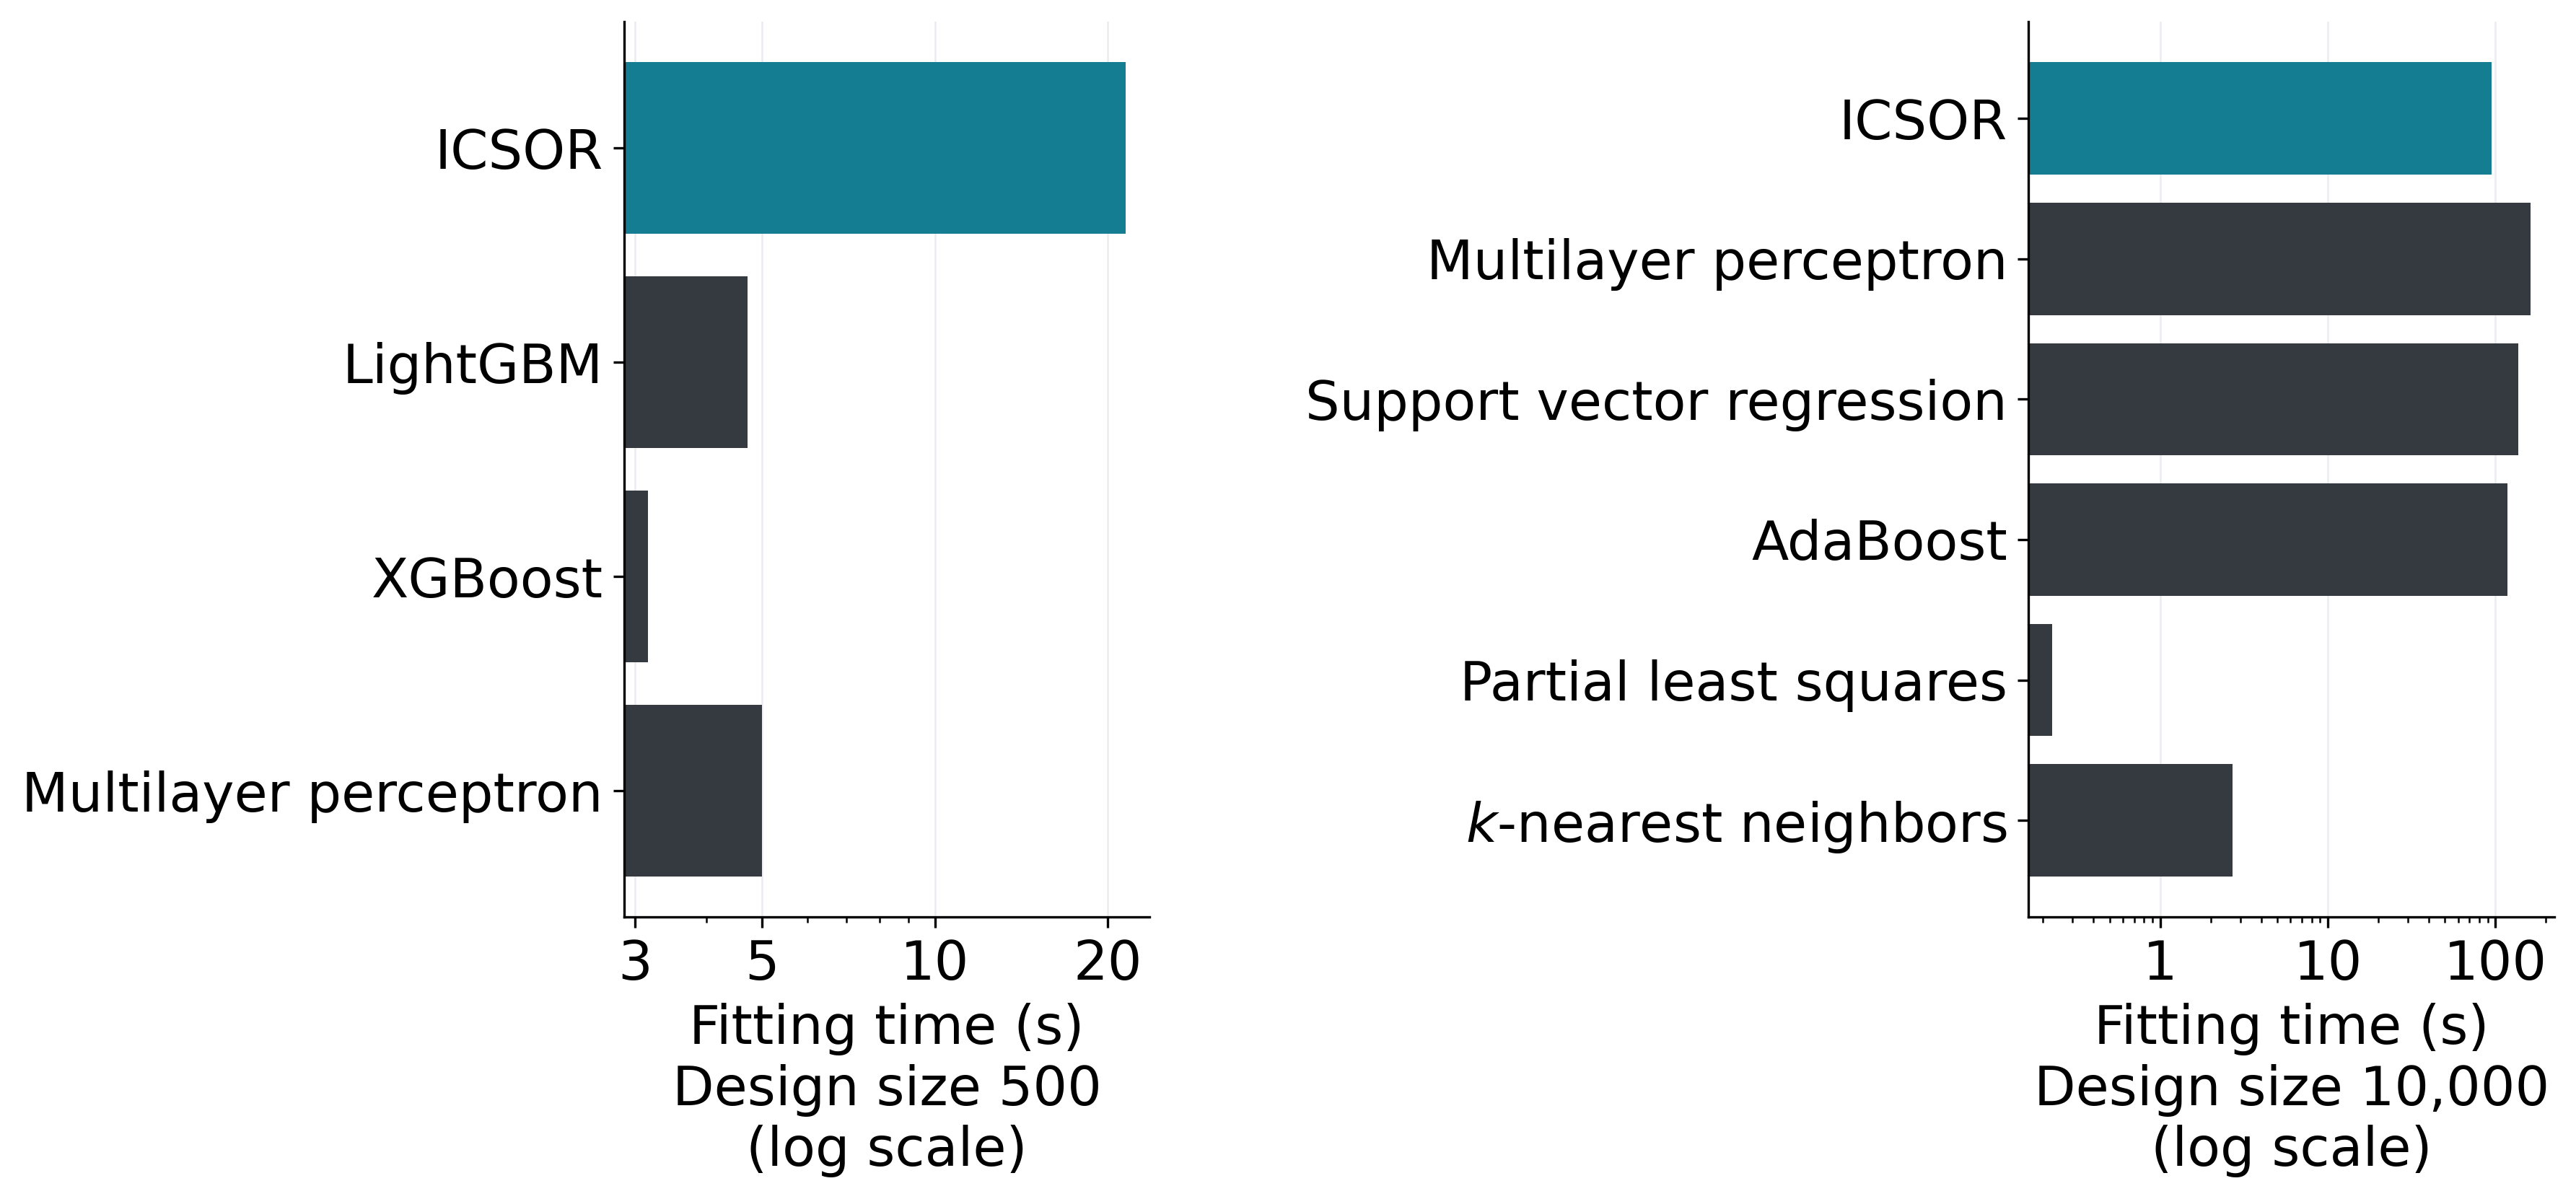
\includegraphics[width=\textwidth]{results/ch5/q06_fitting_effort.png}
\caption{Mean fitting times for the specified predictors at design sizes 500 and 10,000. Teal identifies ICSOR. Each panel uses a logarithmic seconds axis. The values concern repeated model fits and exclude deployment calculations.}
\label{fig:icsor_fitting_results}
\end{figure}

\subsection{Inspectable coefficient structure}

The fitted coefficient structure shows where ICSOR remained selective and where it relied on dense dependence among component channels. Table~\ref{tab:icsor_coefficient_results} reports the COD raw-composite polynomial coefficients together with the shared coupling matrix. The polynomial representation contains 276 unique candidate terms. Adding the 380 off-diagonal coupling entries gives 656 entries in the displayed structure. Under the specified post-fitting thresholds, 469 entries were retained, corresponding to 71.5\% of the combined display.

\begin{table}[htbp]
\centering\small
\caption{Coefficients exceeding the reporting thresholds in one fitted model. Polynomial blocks describe the COD row of $B_{\mathrm{raw,comp}}$. The coupling matrix is shared across component outputs and uses its own threshold. Symmetric quadratic blocks count unique upper-triangular terms.}
\label{tab:icsor_coefficient_results}
\begin{tabular}{p{6.2cm}rrr}
\toprule
Coefficient block & Candidates & Retained & Retained (\%)\\
\midrule
Baseline $b$ & 1 & 1 & 100.0\\
Operating terms $W_u$ & 2 & 2 & 100.0\\
Influent terms $W_{in}$ & 20 & 19 & 95.0\\
Operating curvature $\Theta_{uu}$ & 3 & 3 & 100.0\\
Operating-load interactions $\Theta_{uc}$ & 40 & 29 & 72.5\\
Influent curvature $\Theta_{cc}$ & 210 & 44 & 21.0\\
Shared off-diagonal coupling $\Gamma$ & 380 & 371 & 97.6\\
Combined display & 656 & 469 & 71.5\\
\bottomrule
\end{tabular}
\end{table}

The contrast between influent curvature and component coupling was pronounced. Only 44 of 210 unique influent-curvature terms exceeded the display threshold, whereas 371 of 380 coupling entries did. The fitted representation was therefore selective in its nonlinear influent curvature but dense in the dependence learned among output components. This pattern is important for interpretation because it shows that the visible polynomial structure was not uniformly sparse.

The largest absolute COD influent-curvature coefficient was the dissolved-oxygen self term at \(-5.8097\). The two mirrored dissolved-oxygen--dinitrogen entries were each \(-1.7411\), giving a combined unordered interaction coefficient of \(-3.4822\). Other prominent terms linked dissolved oxygen with metal phosphate, ammonia-oxidizing biomass, soluble phosphate, nitrite-oxidizing biomass, and nitrite. These coefficients belong to the raw COD composite mapping after both component coupling and reporting have been applied.

Figure~\ref{fig:icsor_structure_results} shows the retained counts and selected oxygen-related curvature terms. The plotted interaction values combine the two mirrored cells, consistent with the symmetry convention. The figure therefore describes the fitted polynomial in its native input units rather than implying that coefficient magnitudes from different units are directly comparable.

\begin{figure}[htbp]
\centering
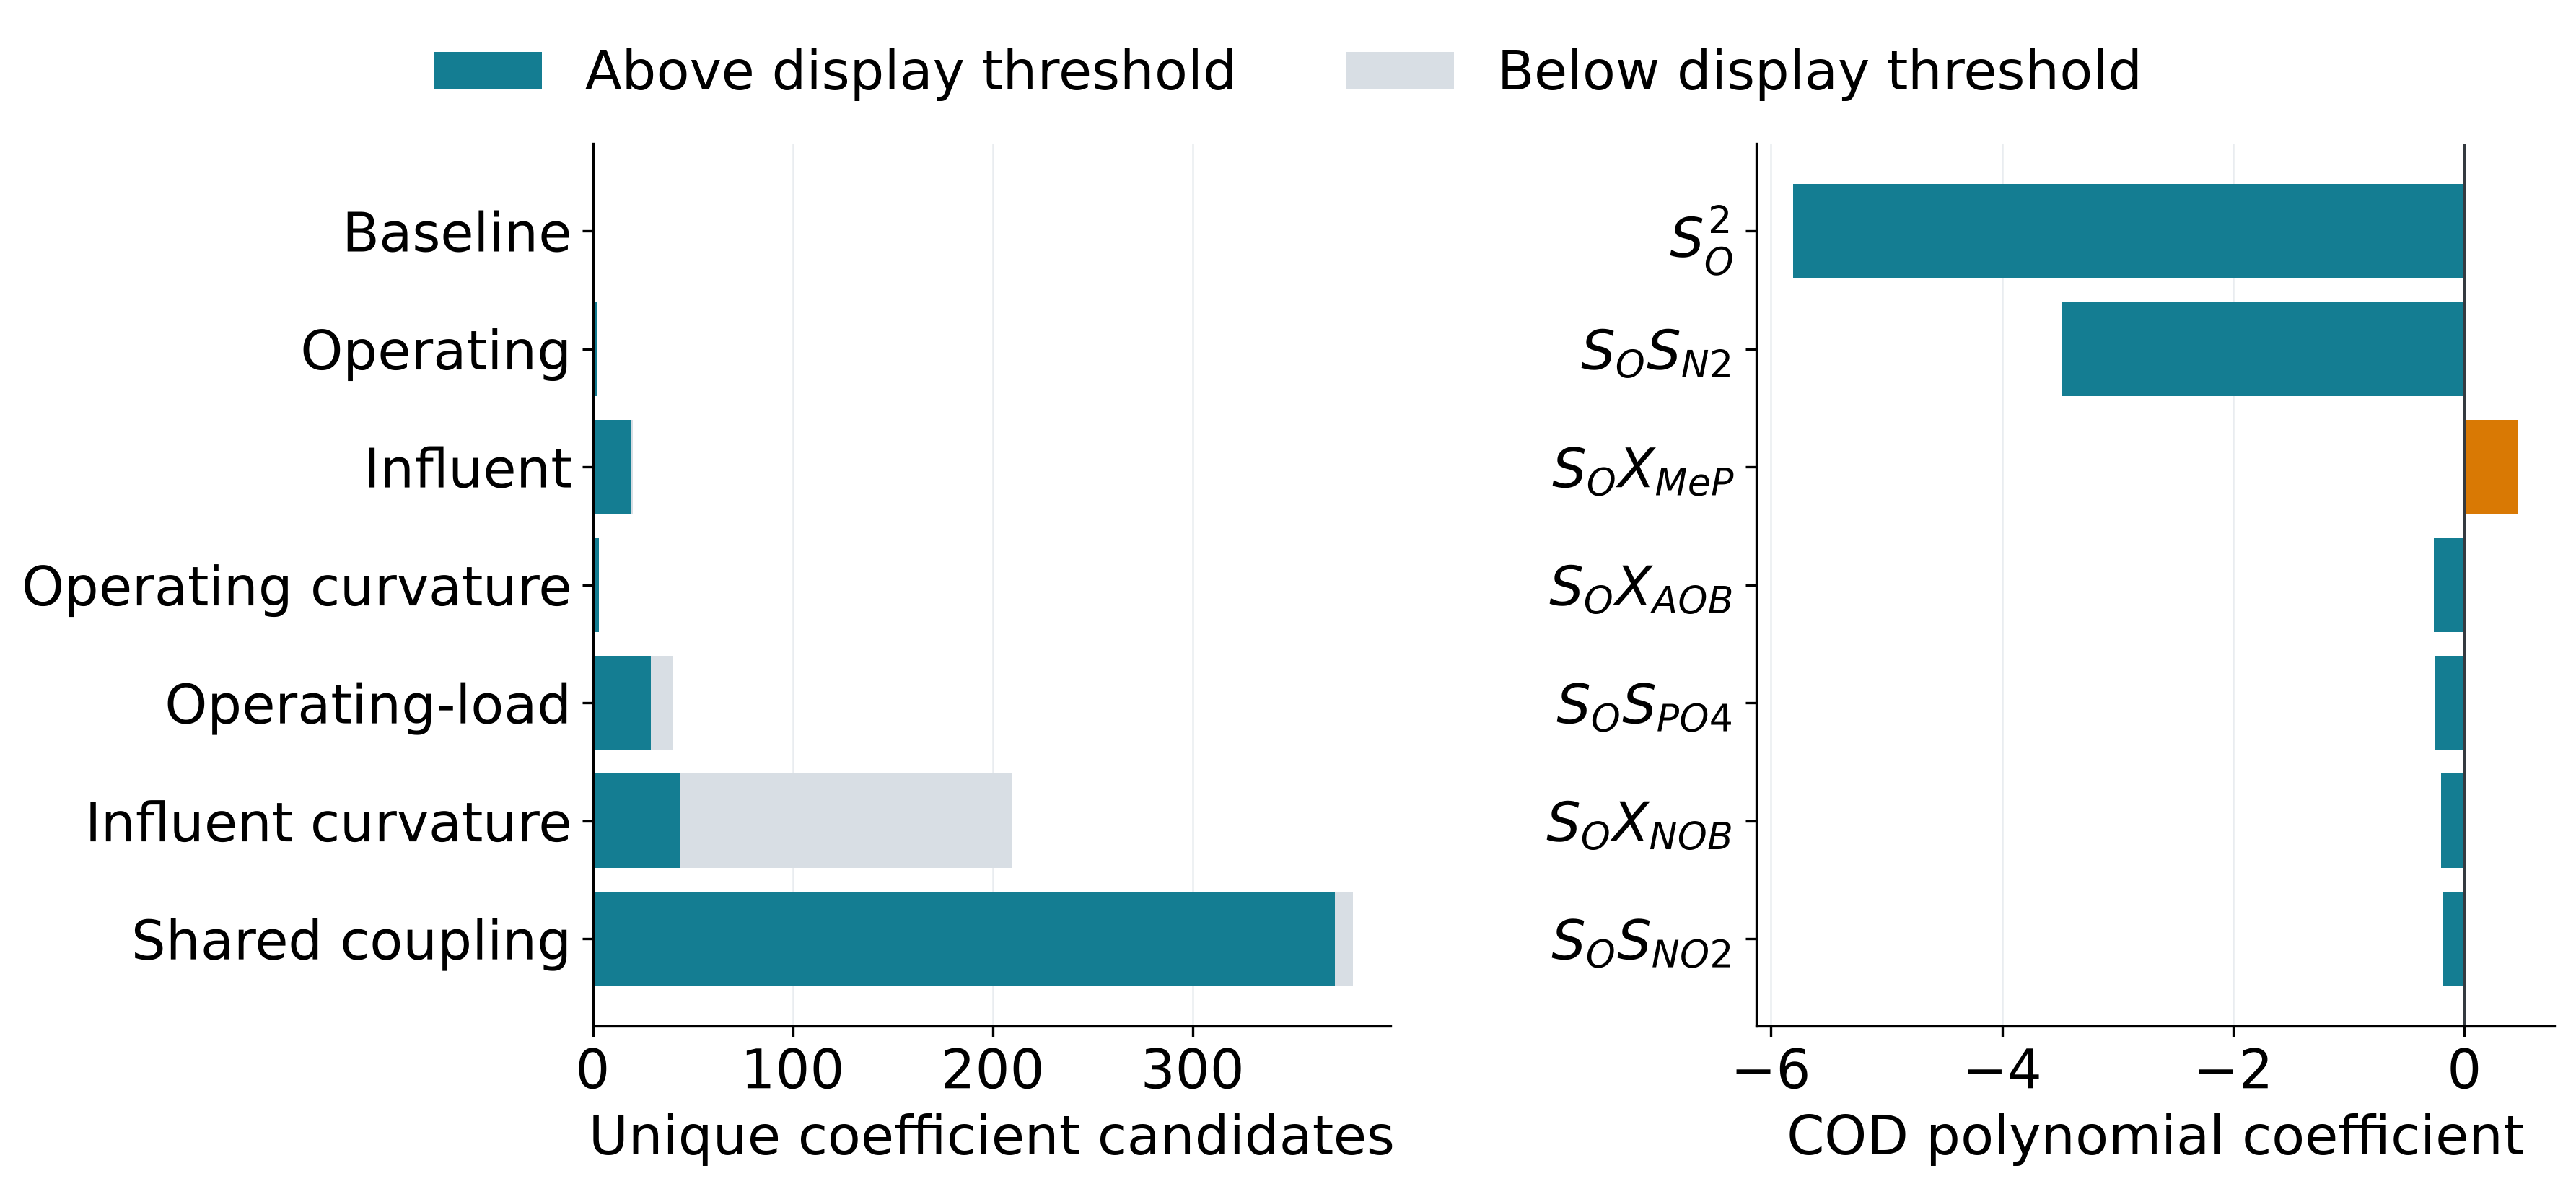
\includegraphics[width=\textwidth]{results/ch5/q07_coefficient_structure.png}
\caption{Coefficient structure of one fitted ICSOR model. The left panel separates entries above and below the display thresholds for the COD polynomial blocks and shared coupling. The right panel shows selected COD influent-curvature coefficients with mirrored interaction entries combined. Coefficient units depend on the corresponding input terms. The displayed values describe the raw composite mapping.}
\label{fig:icsor_structure_results}
\end{figure}

\section{Discussion}
\label{sec:icsor_discussion}

\subsection{A structured approximation under limited data}

The results show that the value of the structured model depends strongly on the available data budget. ICSOR produced the lowest mean held-out root error at the smallest design size and the lowest normalized root-error curve area across the full sample-size range. Its explicit second-order driver, invariant-aware fitting objective, and learned component coupling therefore provided a useful approximation when fewer mechanistic simulations were available. This behavior is consistent with the broader role of model structure in hybrid learning discussed by \citet{Shen2023} and with the changing learner orderings across data budgets reviewed by \citet{VieringLoog2023}.

That advantage did not persist as a universal ranking. At the largest design size, the multilayer perceptron produced the lowest composite error, while LightGBM achieved the best mean dense rank across targets, metrics, and sample sizes. ICSOR's normalized curve area of 6.33 was only slightly lower than LightGBM's 6.35, but its final full-data error remained higher than that of the strongest flexible learners. The result therefore does not support choosing ICSOR simply because it is interpretable. Instead, it identifies a specific trade-off: ICSOR offers an explicit equation, favorable performance when simulations are limited, and checked component states, while more flexible learners can achieve lower prediction error when a larger training design is available \citep{Rudin2019,BhosekarIerapetritou2018}.

The generalization results reinforce the same point. ICSOR's training-to-held-out root-error gap was small, but a small gap is useful only when the underlying prediction error is also acceptable. Partial least squares demonstrated the opposite case: it also had a relatively small gap, yet its held-out error remained high. The leading flexible learners achieved lower absolute error despite larger training-to-held-out differences. Generalization gap and predictive accuracy therefore describe complementary properties and should not be interpreted as substitutes for one another.

From an engineering perspective, the sample-size results provide a practical model-selection rule rather than a universal ranking. When generating mechanistic training cases is costly and only a modest design can be afforded, the structured response can make efficient use of those cases while retaining direct inspectability. When simulation data are abundant and minimum predictive error is the dominant requirement, the results favor the more flexible learners evaluated here. The usefulness of an interpretable surrogate therefore depends on the data available and on whether transparency and physical checking are themselves required properties of the engineering workflow.

\subsection{Fitting guidance and final-state enforcement}

The physical results clarify the different roles of fitting guidance and output enforcement. The invariant penalty influenced the auxiliary training states, and the learned coupled system produced the raw prediction for a new input. Neither step, however, guaranteed that the raw deployed state satisfied the adopted physical requirements. Every raw ICSOR prediction in the fixed held-out set required at least the affine mass-conservation projection.

Projection then supplied the guarantees that fitting alone did not provide. The affine stage restored the adopted balances for every held-out case and was sufficient to return a non-negative state for 21.8\% of the predictions. The remaining 78.2\% required the weighted constrained projection, after which every returned state satisfied both the balance and non-negativity checks. The final zero-violation result is therefore attributable to the checked deployment procedure rather than to the soft penalty used during model fitting. This separation is consistent with the distinction between physics-guided learning and explicit output enforcement examined by \citet{Hansen2024} and \citet{KircherVotsmeier2025}.

This distinction is important because a physically checked output is not the same as a statistically superior output. The same deployment procedure that guarantees the adopted balances can alter concentrations and therefore alter prediction error. The numerical comparison used checked ICSOR states and affine-aligned comparator states for accuracy scoring, while the physical comparator diagnostics intentionally used the raw comparator states. Under this convention, ICSOR had a 36.5\% larger pooled root error than the multilayer perceptron, and all methods shared the same TP error of 0.0361 after alignment and reporting. These outcomes should therefore be read together with the deployment rules that produced them.

The result also shows why physical diagnostics need to identify the stage being assessed. A raw prediction, an affine mass-conserving state, and a jointly constrained final state are different mathematical objects. Reporting only the final zero-violation rate would hide how much correction was required to obtain it. Conversely, reporting only raw violations would ignore the state that the model actually returns to the engineer. The stage-wise analysis makes both facts visible: the statistical model frequently required correction, and the complete deployed procedure successfully supplied that correction.

\subsection{What the coefficient structure explains}

The fitted coefficient blocks make the response more inspectable by separating operating dependence, influent dependence, curvature, operating-load interactions, and component coupling. This explicit organization follows the preference for transparent predictive structures emphasized by \citet{Rudin2019}. It also prevents a regression coefficient from being interpreted outside the calculation in which it operates. A coefficient belongs first to the driver, after which coupling and the reporting map can redistribute its effect across component and composite outputs.

The fitted structure was not uniformly sparse. Most unique influent-curvature terms fell below the display threshold, while almost every off-diagonal coupling coefficient exceeded its separate threshold. The displayed model therefore combined selective nonlinear dependence on the influent with dense learned dependence among effluent components. The 469 retained entries out of 656 displayed candidates describe this contrast, but the threshold itself does not alter the fitted model. It only controls which coefficients are made visible in the summary.

The prominent oxygen-related terms provide a useful example of how the structure can be interpreted without claiming causal parameter identification. Oxygen availability is central to nitrification and interacts with other nutrient-removal pathways \citep{StenstromSong1991,Wentzel1992}. The dissolved-oxygen self term and the oxygen--dinitrogen interaction therefore identify fitted response patterns that can be compared with known process behavior. Their signs and magnitudes remain properties of the statistical mapping in its native units, not estimates of kinetic constants.

The sensitivity analysis extends this interpretation beyond coefficient inspection. A coefficient describes one term in the polynomial, but the local response at an operating point combines linear effects, curvature, interactions, component coupling, and physical projection. The analytical raw Jacobians in Equation~\eqref{eq:icsor_raw_jacobians} include the first three of these stages, while Equation~\eqref{eq:icsor_affine_jacobians} shows how mass conservation modifies those derivatives. The frequent activation of the constrained branch means that active-set effects are also relevant for many final predictions.

Figure~\ref{fig:assessment_branch_sensitivity} demonstrates why this distinction matters. In the illustrative response, a positive raw first-component slope became negative after affine mass-conservation projection and then became zero when the non-negativity boundary activated. A reader who inspected only the raw polynomial coefficient would therefore describe a different local response from the one returned by the deployed model. The interpretability contribution of ICSOR lies in making this entire sequence traceable.

\subsection{Engineering implications}

Taken together, the results define the engineering role of the structured surrogate more clearly than any single accuracy score. ICSOR combined competitive composite prediction, favorable behavior when training data were limited, an explicit response structure, and final component states that satisfied the imposed numerical checks. Its second-order terms and coupling matrix allow an engineer to examine how operating and loading conditions enter the fitted response. Checked deployment then ensures that COD, TN, TP, and TSS are calculated from a component state that satisfies the adopted material accounting and non-negativity requirements.

These benefits are accompanied by computational costs. ICSOR required more fitting time than the fastest tree and linear comparators, although at 10,000 cases it remained faster than AdaBoost, support vector regression, and the multilayer perceptron. More importantly, fitting time does not describe the full cost of using the model. Most fixed-split predictions required the constrained deployment solve after the raw regression had already been evaluated. The computational value of the model must therefore be assessed through both preparation and repeated deployment rather than through regression evaluation alone. This distinction follows the broader surrogate-modeling emphasis on separating model-development cost from repeated-use cost \citep{BhosekarIerapetritou2018,Bliek2023}.

The practical value of ICSOR is therefore conditional rather than absolute. It is not the most accurate predictor at the largest data budget, nor is its raw prediction automatically physically admissible. Its value is that the complete procedure exposes the fitted relationships, identifies where coupling and projection alter those relationships, and returns a component state that passes the declared physical checks. When transparency, limited simulation data, and component-level physical accounting are important, those properties provide engineering criteria that are not captured by prediction error alone.

The broader implication is that interpretability and physical consistency should be treated as properties of the complete deployed calculation. An explicit equation does not remain fully interpretable if later coupling and projection are ignored, and a physically constrained output does not become accurate merely because its balances close. The structured framework makes these distinctions explicit. It allows prediction accuracy, model structure, physical enforcement, and computational effort to be examined together without treating any one of them as evidence for the others.

\subsection{Data Availability}
\label{sec:icsor_data_availability}

The simulation data and numerical results supporting this study are publicly available at \url{https://github.com/egbertoselerio1997/icsor}.
\chapter{Connected plant surrogates and operating optimization}
\label{ch:plant}

\section{From an admissible reactor prediction to a plant decision}

An activated sludge plant repeatedly moves material between biological reactors and a secondary clarifier. Settled biomass returns to the biological treatment train. Mixed liquor may return to an upstream stage to support nitrogen removal. A separate waste stream removes accumulated solids. Aeration, recycle, and wasting therefore affect more than one treatment unit. The account of biological treatment given by \citet{Henze2008} explains why these decisions need a common plant balance. The clarification and thickening model of \citet{HartelPopel1992} adds the storage and separation processes that determine which solids return to the reactors.

The operating question is how to choose these settings while balancing treated-water quality and resource use. \citet{Araujo2013} formulate activated sludge operation as a constrained economic problem and examine the sensitivity of the resulting decisions. \citet{PadronPaez2020} examine wastewater treatment design through multiple objectives. \citet{Aboagye2021} organize treatment-network design and sustainability assessment within mathematical programming. These studies make a common point. A preferred decision depends on the objective, the feasible operating region, and the quantities used to measure treatment and resource use.

A process surrogate can reduce the cost of evaluating the same plant at many candidate settings. \citet{McBride2019} describe surrogate construction from experiments and process simulations. \citet{BhosekarIerapetritou2018} connect surrogate prediction to feasibility analysis and optimization. Applications include the Kriging treatment model of \citet{He2023}, the machine learning process model within predictive control developed by \citet{Bernardelli2020}, and the unit surrogates used for wastewater resource-recovery optimization by \citet{Durkin2024}. Each application links prediction to a decision problem. Its objective and constraints determine which prediction errors matter most.

A physically admissible prediction for one reactor does not by itself establish a consistent plant prediction. The predicted clarifier underflow may disagree with the predicted return-sludge contribution at the mixer. Separate predictions may also assign different amounts of a inventory used for mass conservation to connected streams. ICSOR supplies a useful starting point because it separates second-order statistical prediction from enforcement of declared physical relations \citep{Selerio2026}. Extending this principle to a plant requires a joint response and a joint projection. The projection must account for the mixer, all reactors, both clarifier outlets, and the solids stored in the clarifier.

Three questions remain distinct. A network prediction can satisfy the imposed balances. It can also approximate a mechanistic reference accurately. Finally, it can lead an optimizer to a useful operating decision. None of these properties is a substitute for the others. The surrogate comparisons studied by \citet{Pedrozo2025} make optimization performance a separate endpoint from predictive accuracy. The gray-box methods of \citet{Hameed2026} also retain checks against the original model when managing approximation error. The connected formulation developed here therefore includes independent mechanistic evaluation of selected controls.

\section{Hydraulic connections and reactor inventories}

\subsection{Flow through the treatment train}

Let $Q_0$ denote the fresh-influent flow in m$^3$ d$^{-1}$ and let $c_{\rm in}\in\mathbb R_+^F$ denote its component concentrations. The plant has $n_r$ completely mixed reactors and an $L$-layer clarifier. The reactor concentrations are $c_1,\ldots,c_{n_r}$. The mixer concentration is $m$. Clarifier overflow and underflow concentrations are $c_E$ and $c_U$. The overflow is the final plant outlet, so $c_{\rm out}=c_E$.

The dimensionless ratios $r_I$, $r_R$, and $w$ describe mixed-liquor recycle, return activated sludge, and waste activated sludge flow relative to $Q_0$. Mixed-liquor recycle leaves the final reactor before the clarifier. Return and waste sludge share the clarifier underflow concentration. Each ratio is an actual flow divided by $Q_0$. Denote the train, clarifier-feed, underflow, and overflow flows by $Q_P,Q_C,Q_U,Q_E$. The mixer, reactor splitter, underflow splitter, and external water balance respectively give
\begin{align}
Q_P&=Q_0+r_IQ_0+r_RQ_0,\\
Q_C&=Q_P-r_IQ_0,\\
Q_U&=r_RQ_0+wQ_0,\\
Q_E&=Q_0-wQ_0.
\end{align}
The second equation removes the mixed-liquor recycle before clarification. The third includes both underflow destinations. Dividing each hydraulic balance by $Q_0$ gives
\begin{equation}
q_P=1+r_I+r_R,\qquad q_C=1+r_R,\qquad
q_U=r_R+w,\qquad q_E=1-w.
\label{eq:plant_flows}
\end{equation}
Here $q_P$ is the reactor-train flow ratio and $q_C$ is the clarifier-feed flow ratio. The identity $q_C=q_E+q_U$ confirms the clarifier water balance. The adopted domain requires $r_I\ge0$, $r_R\ge0$, $0\le w<1$, and $q_U>0$. The outlet concentrations are then defined by positive outlet flows.

Figure~\ref{fig:plant_configuration} places these flow balances on the physical connections of the five-reactor plant. The two recycle routes return material to the mixer, while treated water and waste sludge cross the external boundary.

\begin{figure}[htbp]
\centering
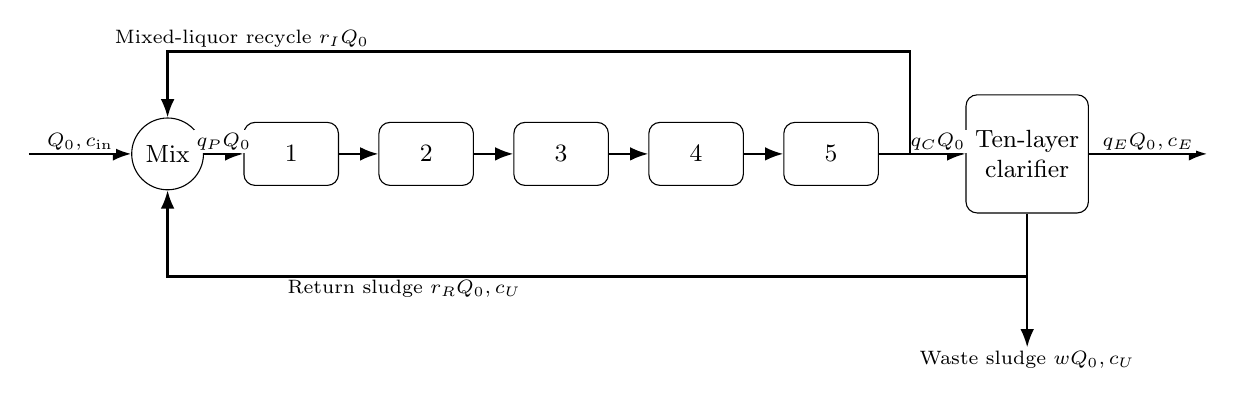
\begin{tikzpicture}[>=Latex,node distance=5mm,
unit/.style={draw,rounded corners,minimum width=12mm,minimum height=8mm,align=center,font=\small},
mix/.style={draw,circle,minimum size=9mm,font=\small},
flow/.style={->,thick},lab/.style={font=\scriptsize,fill=white,inner sep=1pt}]
\node[mix] (m) {Mix};
\node[unit,right=of m] (r1) {1};
\node[unit,right=of r1] (r2) {2};
\node[unit,right=of r2] (r3) {3};
\node[unit,right=of r3] (r4) {4};
\node[unit,right=of r4] (r5) {5};
\coordinate[right=4mm of r5] (split);
\node[unit,right=7mm of split,minimum height=15mm] (cl) {Ten-layer\\clarifier};
\draw[flow] ([xshift=-13mm]m.west)--(m.west) node[midway,above,lab] {$Q_0,c_{\rm in}$};
\draw[flow] (m)--(r1) node[midway,above,lab] {$q_PQ_0$};
\draw[flow] (r1)--(r2); \draw[flow] (r2)--(r3);
\draw[flow] (r3)--(r4); \draw[flow] (r4)--(r5);
\draw[thick] (r5)--(split);
\draw[flow] (split)--(cl) node[midway,above,lab] {$q_CQ_0$};
\draw[flow] (split)--++(0,13mm)-|(m.north) node[pos=.45,above,lab] {Mixed-liquor recycle $r_IQ_0$};
\draw[flow] (cl.east)--++(15mm,0) node[midway,above,lab] {$q_EQ_0,c_E$};
\draw[thick] (cl.south)--++(0,-8mm) coordinate (u);
\draw[flow] (u)--++(0,-9mm) node[below,lab] {Waste sludge $wQ_0,c_U$};
\draw[flow] (u)--++(-9mm,0)-|(m.south) node[pos=.35,below,lab] {Return sludge $r_RQ_0,c_U$};
\end{tikzpicture}
\caption{Connected plant configuration used for the operating study. Reactors 1 and 2 are unaerated. Reactors 3--5 have independent aeration controls.}
\label{fig:plant_configuration}
\end{figure}

The diagram shows why the reactor-train and clarifier-feed flows differ. Mixed-liquor recycle leaves before the clarifier, while return sludge leaves the clarifier underflow. Their concentrations consequently come from different locations. The mixer calculation uses each stream's own flow and concentration rather than assigning one shared recycle concentration.

The mixer balance is a component balance rather than a balance of a single water-quality total. For component $f$, its incoming and outgoing mass rates satisfy
\begin{equation}
Q_Pm_f=Q_0c_{{\rm in},f}+r_IQ_0c_{n_r,f}+r_RQ_0c_{U,f}.
\end{equation}
Each product has units of g d$^{-1}$ when the component basis is g m$^{-3}$. Divide by $Q_0$ and then by $q_P$ to obtain
\begin{equation}
m_f=\frac{c_{{\rm in},f}+r_Ic_{n_r,f}+r_Rc_{U,f}}{1+r_I+r_R}.
\end{equation}
For two components, the same calculation is performed independently in each row,
\begin{equation}
\begin{bmatrix}q_P&0\\0&q_P\end{bmatrix}
\begin{bmatrix}m_1\\m_2\end{bmatrix}
=\begin{bmatrix}c_{{\rm in},1}+r_Ic_{n_r,1}+r_Rc_{U,1}\\
c_{{\rm in},2}+r_Ic_{n_r,2}+r_Rc_{U,2}\end{bmatrix}.
\end{equation}
The complete concentration vector therefore satisfies
\begin{equation}
q_Pm=c_{\rm in}+r_Ic_{n_r}+r_Rc_U.
\label{eq:plant_mixer}
\end{equation}
A high mixer concentration can therefore result from internal circulation. It does not imply that an external pollutant load has been created. The component-resolved framework of \citet{Zhang2026} treats these recirculation and discharge streams explicitly.

A hypothetical mixing calculation makes the units and recycle effect explicit. Let $Q_0=10{,}000$ m$^3$ d$^{-1}$, $r_I=2$, $r_R=0.5$, and $w=0.02$. The four physical flows are $35{,}000$, $15{,}000$, $5{,}200$, and $9{,}800$ m$^3$ d$^{-1}$ in the order $Q_P,Q_C,Q_U,Q_E$. For one particulate component, specify fresh, final-reactor, and underflow concentrations of 200, 1{,}000, and 2{,}000 g m$^{-3}$. The mixer calculation is
\begin{align}
q_Pm_f&=200+2(1{,}000)+0.5(2{,}000)=3{,}200,\\
m_f&=3{,}200/3.5=914.29\ \mathrm{g\,m^{-3}}.
\end{align}
The physical incoming mass rates are 2{,}000, 20{,}000, and 10{,}000 kg d$^{-1}$. Their sum is the 32{,}000 kg d$^{-1}$ leaving the mixer. The mixer concentration exceeds the fresh concentration because the two return streams contain concentrated material. These specified streams illustrate mixing and do not constitute a complete calculated plant state.

The nominal stage HRT is measured on the fresh-flow basis. A volume divided by a flow gives time. Thus $V_i/Q_0$ has units of days, and multiplying by 24 converts it to hours. The actual flow through the reactor is $Q_P=Q_0q_P$, so its actual residence time is $V_i/Q_P$. The inverse of that actual time is the dilution rate. With reactor volume $V_i$,
\begin{equation}
h_i=\frac{24V_i}{Q_0},\qquad H=\sum_{i=1}^{n_r}h_i,\qquad
d_i=\frac{Q_0q_P}{V_i}=\frac{24q_P}{h_i}.
\label{eq:plant_residence}
\end{equation}
The factors $h_i$ and $H$ are in hours. The dilution rate $d_i$ is in d$^{-1}$. The actual residence time during one passage through stage $i$ is $h_i/q_P$. For a hypothetical plant with $H=24$ h, $r_I=2$, and $r_R=0.5$, the reactor-train flow ratio is 3.5. Its train residence time per passage is about 6.86 h. Equal tanks then have a residence time per passage of about 1.37 h. These illustrative numbers explain why nominal HRT and recycle flow must be interpreted together.

Fixed stage fractions can be represented by $h_i=f_i^V H$, where $f_i^V>0$ and $\sum_i f_i^V=1$. The case study uses equal fractions. Varying $H$ at fixed $Q_0$ varies biological reactor volume. The resulting problem combines capacity selection and operating decisions. For an existing plant with installed tanks, the volumes would be fixed and $H$ would be removed from the free-control vector.

Let $\vartheta$ collect only settings that vary freely. A constant setting remains a parameter. Treating it as a varying regression coordinate would create a zero-variance feature. A carbon or chemical addition may also enter the control vector. An addition represented only by a source term has negligible liquid carrier flow. An appreciable carrier flow requires a new hydraulic stream and revised downstream dilution rates.

\subsection{Biological conversion and non-negativity}

The reaction network uses the component and process representation of Chapter~\ref{ch:foundations}. Its stoichiometric matrix is $\nu\in\mathbb R^{P\times F}$ and its process-rate vector in stage $i$ is $\rho_i\in\mathbb R_+^P$. For component $f$, the dynamic mass balance is
\begin{equation}
V_i\frac{dc_{i,f}}{dt}=Q_Pc_{i-1,f}-Q_Pc_{i,f}
+V_i\sum_{p=1}^{P}\nu_{pf}\rho_{i,p}+V_i\omega_i(e_{S_O})_f+V_i\xi_{i,f}.
\end{equation}
The reaction sum combines the change caused by each process. A negative $\nu_{pf}$ consumes component $f$, while a positive entry produces it. The oxygen selector is one for the oxygen component and zero elsewhere. At steady state, the accumulation term is zero. Dividing the remaining equation by $V_i$ gives
\begin{equation}
0=d_i(c_{i-1,f}-c_{i,f})+\sum_{p=1}^{P}\nu_{pf}\rho_{i,p}
+\omega_i(e_{S_O})_f+\xi_{i,f}.
\end{equation}
Putting all $F$ component equations into one vector gives the steady reactor equation, with $c_0=m$,
\begin{equation}
0=d_i(c_{i-1}-c_i)+\nu^\top\rho_i(c_i,\vartheta)
+k_La_i(a_i)(S_O^*-c_{i,S_O})e_{S_O}+\xi_i(\vartheta).
\label{eq:plant_reactor}
\end{equation}
The vector $e_{S_O}$ selects dissolved oxygen. The parameter $S_O^*$ is its saturation concentration. The vector $\xi_i$ represents declared stage additions. Each term has units of component concentration per day. The treatment-model framework of \citet{Henze2006} separates hydraulic transport, stoichiometric conversion, and external sources in this way.

At a zero component concentration, the combined reaction and external-source terms must not direct that component below zero. With non-negative inflow and a locally Lipschitz balance function defined on the boundary, this condition preserves the non-negative state space of the dynamic model \citep{Haddad2010}. A numerical integrator does not inherit this property automatically. Acceptance therefore checks concentrations and reaction rates independently of the solver's stopping message.

The same distinction matters for a surrogate. A fitted quadratic equation can predict a negative concentration even when every training state is non-negative. Polynomial approximation imposes no sign restriction. The work of \citet{KircherVotsmeier2025} addresses the simultaneous requirements of mass conservation and non-negativity in kinetic surrogates. Both requirements need explicit treatment.

\subsection{Stage invariants and the external plant balance}

Consider a hypothetical reaction that transfers material from component 1 to component 2 without changing their combined amount. Its stoichiometric and inventory rows are
\begin{equation}
\nu=\begin{bmatrix}-1&1\end{bmatrix},\qquad
A=\frac1{\sqrt2}\begin{bmatrix}1&1\end{bmatrix}.
\end{equation}
The factor $1/\sqrt2$ gives the inventory row unit length. Matrix multiplication shows the cancellation directly,
\begin{equation}
A\nu^\top=\frac1{\sqrt2}\left[1(-1)+1(1)\right]=0.
\end{equation}
At an illustrative dilution rate of 2 d$^{-1}$, take upstream concentrations $(12,3)$ and downstream concentrations $(8,7)$ g m$^{-3}$, with a reaction rate of 8 g m$^{-3}$ d$^{-1}$. The component equations are
\begin{align}
0&=2(12-8)-8,\\
0&=2(3-7)+8.
\end{align}
Adding them removes the unknown reaction rate. Both upstream and downstream totals are 15 g m$^{-3}$. The normalized invariant is that total divided by $\sqrt2$. The full reactor model applies the same cancellation to more components and more processes.

Let $A\in\mathbb R^{K\times F}$ contain independent inventory rows such that
\begin{equation}
A\nu^\top=0,\qquad Ae_{S_O}=0,\qquad
\operatorname{rank}(A)=K.
\label{eq:plant_invariant_operator}
\end{equation}
The rows are normalized to unit Euclidean length. Unit row normalization does not make them orthogonal. Physically named inventories and an orthonormal basis can span the same subspace defined by mass conservation while using different coordinates. The stoichiometric fixed-layer formulation of \citet{SturmWexler2022} illustrates the value of separating quantities used for mass conservation from the rates that redistribute them.

For inventory row $k$, multiply component equation $f$ by $A_{kf}$ and sum over $f$. The reaction contribution becomes
\begin{equation}
\sum_{f=1}^{F}A_{kf}\sum_{p=1}^{P}\nu_{pf}\rho_{i,p}
=\sum_{p=1}^{P}\left(\sum_{f=1}^{F}A_{kf}\nu_{pf}\right)\rho_{i,p}=0.
\end{equation}
The inner sum is entry $(k,p)$ of $A\nu^\top$. Oxygen transfer also disappears because $Ae_{S_O}=0$. The remaining scalar equation is
\begin{equation}
d_i\left(\sum_fA_{kf}c_{i-1,f}-\sum_fA_{kf}c_{i,f}\right)
+\sum_fA_{kf}\xi_{i,f}=0.
\end{equation}
Moving the transport difference to the other side and dividing by the positive $d_i$ gives the remaining stage relation,
\begin{equation}
A(c_i-c_{i-1})=d_i^{-1}A\xi_i(\vartheta).
\label{eq:plant_invariant_transition}
\end{equation}
If there is no stage addition, $Ac_i=Ac_{i-1}$. For example, nitrification can transfer nitrogen from ammonium to oxidized forms while denitrification transfers it to dissolved nitrogen gas. These changes do not remove nitrogen from the model's complete nitrogen inventory. A reporting quantity that excludes dissolved nitrogen gas can decrease while the inventory used for mass conservation remains unchanged. Nutrient-form interpretation in \citet{USEPA2009} supports the need to inspect individual species as well as reported totals.

In the two-component example, adding component 1 at 2 g m$^{-3}$ d$^{-1}$ changes the downstream concentrations to $(9,7)$ when the same reaction rate is used. The two balances are $2(12-9)-8+2=0$ and $2(3-7)+8=0$. Their total changes by $2/2=1$ g m$^{-3}$. Thus the invariant transition must include a dose whenever that dose carries the quantity used for mass conservation. A zero invariant difference would incorrectly remove the added material.

Internal recycle streams also cancel from an external invariant balance. First add the stage transitions. Every intermediate $Ac_i$ appears once with a plus sign and once with a minus sign. This gives
\begin{align}
A(c_{n_r}-m)&=\sum_i\frac{V_i}{Q_0q_P}A\xi_i,\\
q_PAc_{n_r}-q_PAm&=D_{\rm add},\qquad
D_{\rm add}=\sum_i\frac{V_i}{Q_0}A\xi_i.
\end{align}
Next multiply the mixer balance by $A$ and substitute it for $q_PAm$,
\begin{align}
q_PAc_{n_r}&=Ac_{\rm in}+r_IAc_{n_r}+r_RAc_U+D_{\rm add},\\
(q_P-r_I)Ac_{n_r}&=Ac_{\rm in}+r_RAc_U+D_{\rm add}.
\end{align}
Since $q_P-r_I=q_C$, the left-hand side is the clarifier-feed inventory flow. The clarifier balance gives a second expression for that same quantity,
\begin{equation}
q_CAc_{n_r}=q_EAc_E+(r_R+w)Ac_U.
\end{equation}
Equating the expressions and subtracting $r_RAc_U$ cancels the return-sludge flow. The mixed-liquor recycle already canceled in $q_P-r_I$. The remaining external relation is
\begin{equation}
Ac_{\rm in}+\sum_{i=1}^{n_r}\frac{V_i}{Q_0}A\xi_i
=q_EAc_E+wAc_U.
\label{eq:plant_external_invariant}
\end{equation}
Only fresh feed, stage additions, effluent, and waste sludge remain. The recycle ratios still influence the state and treatment processes. Their cancellation means that they are internal transfers rather than external sources or sinks.

For ASM2d-TSN, $F=20$, $P=28$, and $K=5$. The five inventories concern soluble inert material, total nitrogen including dissolved nitrogen gas, total phosphorus, an alkalinity-related combination, and a metal-related combination. The last two unnormalized combinations are
\begin{align}
I_{\rm alk}&=S_{ALK}-\frac{S_{NH4}}{14}
+\frac{S_{NO2}}{14}+\frac{S_{NO3}}{14}-\frac{S_{PO4}}{31},\\
I_{\rm metal}&=3.45X_{MeP}+4.87X_{MeOH}.
\label{eq:plant_named_invariants}
\end{align}
The nitrogen and phosphorus rows use the constituent weights in Table~\ref{tab:component_basis_composites}. The nitrogen inventory also gives dissolved nitrogen gas unit weight. The stoichiometric rank is 15 under the stated parameterization. The inventory identities are audited rather than inferred from a reporting label such as TN.

\section{Clarification, component separation, and stored solids}

\subsection{A nonreactive separator with two outlet flows}

The clarifier uses a nonreactive settling representation. Soluble components follow the liquid. Particulate components can settle and concentrate in the underflow. \citet{Takacs1991} provide the settling and thickening formulation used for the aggregate solids profile. \citet{JeppssonDiehl1996} explain why component propagation through a clarifier requires attention beyond a single aggregate solids concentration.

Selection means taking designated entries of a vector without changing them. For the illustrative order $(S_A,S_{NH4},X_H,X_I)$, the two selector matrices are
\begin{equation}
E_S=\begin{bmatrix}1&0&0&0\\0&1&0&0\end{bmatrix},\qquad
E_X=\begin{bmatrix}0&0&1&0\\0&0&0&1\end{bmatrix}.
\end{equation}
Thus $E_Sc=(S_A,S_{NH4})^\top$ and $E_Xc=(X_H,X_I)^\top$. Transposing a selector puts selected entries back into their original positions and fills the other positions with zeros. In this example,
\begin{equation}
E_S^\top E_S=\operatorname{diag}(1,1,0,0),\qquad
E_X^\top E_X=\operatorname{diag}(0,0,1,1).
\end{equation}
Their sum is the identity matrix because every component belongs to exactly one group. Their cross-product is zero because the groups do not overlap. For the complete ordered model, $E_S=[I_{10}\ 0]$ and $E_X=[0\ I_{10}]$. In general, let $E_S\in\mathbb R^{F_S\times F}$ and $E_X\in\mathbb R^{F_X\times F}$ select soluble and particulate components. They satisfy
\begin{equation}
E_S^\top E_S+E_X^\top E_X=I_F,\qquad E_SE_X^\top=0.
\end{equation}
The column $t_X$ maps component concentrations to TSS. Its entries are non-negative and its soluble entries are zero.

For the four-component order above, $t_X=(0,0,0.90,0.75)^\top$. If $X_H=100$ and $X_I=40$ g COD m$^{-3}$, the TSS calculation is $0.90(100)+0.75(40)=120$ g TSS m$^{-3}$. The two factors convert component COD bases to suspended-solids mass. Adding the native numerical concentrations without these conversion factors would give a different quantity.

For one component, the clarifier mass balance in physical flows is
\begin{equation}
Q_Cc_{n_r,f}=Q_Ec_{E,f}+Q_Uc_{U,f}.
\end{equation}
The statistical response uses component flows divided by $Q_0$,
\begin{equation}
g_E=q_Ec_E,\qquad g_U=q_Uc_U.
\label{eq:plant_outlet_flows}
\end{equation}
Their units are the same as concentration because the flow ratios are dimensionless. The actual component discharge rates are $Q_0g_E$ and $Q_0g_U$. Writing balances in these coordinates avoids dividing by a small underflow ratio inside the equality system. The component balance and soluble pass-through are
\begin{equation}
g_E+g_U=q_Cc_{n_r},\qquad
E_Sg_U=q_UE_Sc_{n_r}.
\label{eq:plant_clarifier_equalities}
\end{equation}
The two relations imply $E_Sg_E=q_EE_Sc_{n_r}$. Settling therefore cannot remove a soluble nutrient directly in this model.

For a soluble component $f$, pass-through fixes $c_{U,f}=c_{n_r,f}$. Substitute $g_{U,f}=q_Uc_{n_r,f}$ into the total balance to obtain
\begin{align}
g_{E,f}&=(q_C-q_U)c_{n_r,f}=q_Ec_{n_r,f},\\
c_{E,f}&=g_{E,f}/q_E=c_{n_r,f}.
\end{align}
For a hypothetical feed concentration of 20 g m$^{-3}$ and flow ratios $q_C=1.5$, $q_U=0.52$, and $q_E=0.98$, the feed, underflow, and overflow component flows are 30, 10.4, and 19.6 g m$^{-3}$ on the fresh-flow basis. Both outlet concentrations remain 20 g m$^{-3}$.

The particulate densification requirement is
\begin{equation}
E_Xg_U\ge q_UE_Xc_{n_r}.
\label{eq:plant_densification}
\end{equation}
After division by $q_U$, each underflow particulate concentration is at least its feed concentration. Non-negative overflow and the total component balance also prevent the underflow from recovering more than the incoming particulate flow.

For an illustrative particulate component, take $q_C=1.5$, $q_U=0.52$, and feed concentration 100 g m$^{-3}$. Densification requires $g_U\ge52$ g m$^{-3}$ on the fresh-flow basis. Mass conservation and non-negative overflow require $g_U\le150$ g m$^{-3}$. Thus the underflow recovery fraction lies between $0.52/1.5$ and one. A soluble component with the same feed concentration instead has $g_U=52$ and unchanged soluble outlet concentrations. These examples concern the constraints alone and do not predict a settling-model outcome.

An admissible illustrative choice within that particulate interval is $g_U=140$. Mass conservation then gives $g_E=150-140=10$. Dividing by the respective flow ratios gives $c_U=140/0.52=269.23$ and $c_E=10/0.98=10.20$ g m$^{-3}$. The underflow has recovered $140/150=93.33\%$ of the incoming component flow. The concentrations alone do not give that recovery fraction because the outlet water flows differ.

For any particulate component with positive feed concentration, the same reasoning gives
\begin{equation}
\frac{q_U}{q_C}\le\frac{g_{U,f}}{q_Cc_{n_r,f}}\le1.
\end{equation}
Multiplication by the non-negative TSS weights preserves inequalities. Hence $X_U\ge X_N$. The solids balance $q_CX_N=q_EX_E+q_UX_U$ then gives
\begin{equation}
q_EX_E\le(q_C-q_U)X_N=q_EX_N.
\end{equation}
Division by $q_E>0$ establishes the other endpoint ordering.

Applying $t_X$ gives feed and outlet solids concentrations
\begin{equation}
X_N=t_X^\top c_{n_r},\qquad
X_E=\frac{t_X^\top g_E}{q_E},\qquad
X_U=\frac{t_X^\top g_U}{q_U}.
\label{eq:plant_tss_endpoints}
\end{equation}
The declared constraints imply $X_E\le X_N\le X_U$. They bound separation but do not determine its magnitude. The nonlinear settling calculation and an empirical endpoint model supply additional information through different routes.

\subsection{The layer-resolved mechanistic model}

Clarifier layers are numbered from the surface to the hopper. Their TSS concentrations are $s_1,\ldots,s_L$, with $s_1=X_E$ and $s_L=X_U$. The exact settling velocity at concentration $s$ is
\begin{equation}
v(s,X_N)=\max\left\{0,\min\left[v_{\max},
v_0\left(e^{-r_h(s-f_{\rm ns}X_N)}-e^{-r_p(s-f_{\rm ns}X_N)}\right)\right]\right\}.
\label{eq:plant_settling_velocity}
\end{equation}
The gravitational solids flux is $sv(s,X_N)$. The nonsettleable fraction $f_{\rm ns}$ makes the settling offset depend on the feed concentration. At an interface, a receiver concentration above $X_t$ activates a limitation by the smaller adjacent gravitational flux. Otherwise, the upper-layer gravitational flux passes to the receiver. Hydraulic transport uses the overflow velocity above the feed layer and the underflow velocity below it.

Each finite-volume layer equation is its incoming solids flux minus its outgoing solids flux, multiplied by $A_{\rm cl}/V_{{\rm cl},\ell}$. The feed layer also receives $Q_0q_CX_N/V_{{\rm cl},\ell_F}$. Internal interface fluxes cancel when these equations are summed. At steady state, the resulting total solids balance agrees with Equation~\eqref{eq:plant_clarifier_equalities} after application of $t_X$.

A three-layer illustration shows that cancellation without hiding it inside a summation. Place the feed in layer 2. Let $B_{12}$ be the net solids rate from layer 2 toward layer 1 and $B_{23}$ the net rate from layer 2 toward layer 3. These signed rates combine hydraulic and gravitational transport in g d$^{-1}$. The layer mass equations are
\begin{align}
V_1\dot s_1&=B_{12}-Q_Es_1,\\
V_2\dot s_2&=Q_CX_N-B_{12}-B_{23},\\
V_3\dot s_3&=B_{23}-Q_Us_3.
\end{align}
Adding them removes both interface rates. At steady state, the remaining equation is $Q_CX_N=Q_EX_E+Q_UX_U$. This cancellation holds even though the interface rates depend nonlinearly on the neighboring concentrations. Mass conservation of the whole clarifier therefore does not determine its internal fluxes or profile.

The mechanistic state retains one solids concentration per layer. It does not retain a separate transient concentration for every particulate species in every layer. At a steady state, particulate outlet components are reconstructed with the final-reactor particulate composition,
\begin{equation}
E_Xc_E=\frac{s_1}{X_N}E_Xc_{n_r},\qquad
E_Xc_U=\frac{s_L}{X_N}E_Xc_{n_r}.
\label{eq:plant_outlet_reconstruction}
\end{equation}
Soluble outlet components equal their feed concentrations. This reduced representation defines the physical scope of the mechanistic reference. Its steady component mapping is well defined when $X_N>0$. It does not establish the dynamic propagation of each particulate species considered in more detailed component-transport models \citep{JeppssonDiehl1996}.

\subsection{An exact interval for aggregate inventory under the endpoint envelope}

Inventory is concentration multiplied by volume, summed over the vessel. For an illustrative four-layer clarifier, it is
\begin{equation}
M=V_1X_E+V_2s_2+V_3s_3+V_4X_U.
\end{equation}
For example, four 100-m$^3$ layers with concentrations $(10,200,600,1{,}000)$ g m$^{-3}$ store $100(10+200+600+1{,}000)=181{,}000$ g, or 181 kg. The general clarifier's stored solids mass is
\begin{equation}
M_{\rm cl}=\sum_{\ell=1}^{L}V_{{\rm cl},\ell}s_\ell,\qquad
V_{\rm cl}=\sum_{\ell=1}^{L}V_{{\rm cl},\ell}.
\label{eq:plant_inventory_definition}
\end{equation}
An outlet concentration cannot determine this mass. Two clarifiers can have the same endpoints and different internal storage. Whole-plant solids retention time therefore requires the inventory as well as the two outlet solids flows. The benchmark formulation of \citet{Alex2008} includes reactor and settler inventories in its sludge-age calculation.

The mechanistic acceptance envelope requires
\begin{equation}
X_E\le s_\ell\le X_U,\qquad \ell=2,\ldots,L-1.
\label{eq:plant_layer_envelope}
\end{equation}
This is an endpoint envelope. It does not require monotonic concentration from one layer to the next. With positive layer volumes, minimizing the inventory assigns every internal layer $X_E$. Maximizing it assigns every internal layer $X_U$.

For four layers, the envelope bounds each of the two unknown terms separately,
\begin{align}
V_2X_E+V_3X_E&\le V_2s_2+V_3s_3\\
&\le V_2X_U+V_3X_U.
\end{align}
Adding the known endpoint terms gives
\begin{align}
(V_1+V_2+V_3)X_E+V_4X_U&\le M,\\
M&\le V_1X_E+(V_2+V_3+V_4)X_U.
\end{align}
For the hypothetical four equal layers above, these values are 103{,}000 and 301{,}000 g. The 181{,}000-g inventory lies inside the interval. If both internal concentrations were instead 400 g m$^{-3}$, the mass would still be 181{,}000 g. Thus matching endpoints and total inventory does not identify the internal distribution.

Figure~\ref{fig:plant_inventory_envelope} shows the same four-layer arithmetic as concentration bars. Changing the two internal layers changes stored mass while the surface and hopper concentrations remain fixed. The left and right panels attain the lower and upper interval endpoints derived from the envelope.

\begin{figure}[htbp]
\centering
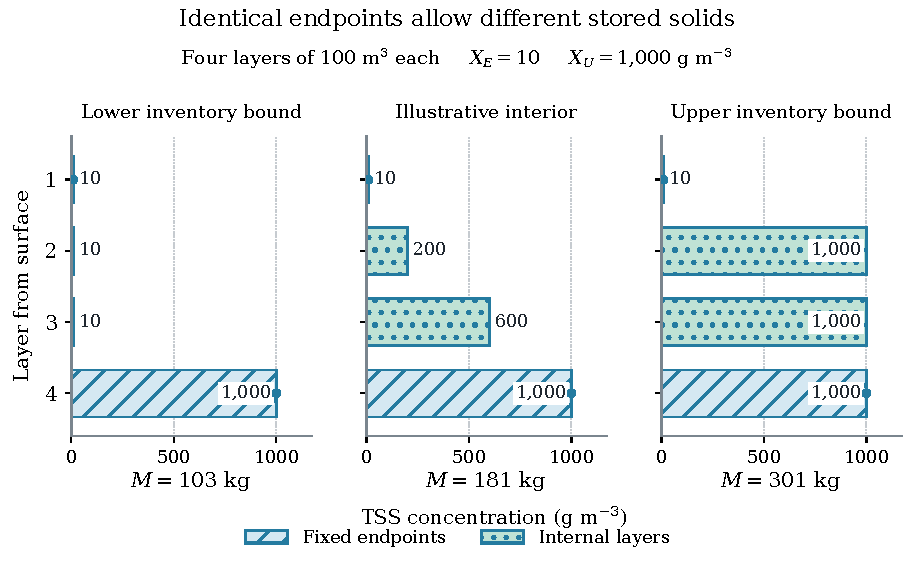
\includegraphics[width=\linewidth]{ch6_concept_inventory_envelope.pdf}
\caption{Hypothetical four-layer profiles with identical overflow and underflow concentrations. Each layer has volume 100 m$^3$. The lower-bound, illustrative interior, and upper-bound profiles store 103, 181, and 301 kg of solids. Hatching identifies the fixed endpoints, while dotted fills identify internal layers. The diagram represents the adopted endpoint envelope and does not assert satisfaction of nonlinear settling equations.}
\label{fig:plant_inventory_envelope}
\end{figure}

The internal layers in the middle panel need not resemble those of another profile with the same inventory. Their total mass is the retained scalar information. The nonlinear layer equations supply the additional information needed to determine a mechanistic profile.

With $L$ layers, the identical argument replaces $V_2+V_3$ by $\sum_{\ell=2}^{L-1}V_{{\rm cl},\ell}$. That internal-volume sum is $V_{\rm cl}-V_{{\rm cl},1}-V_{{\rm cl},L}$. Collecting coefficients of each endpoint gives the general interval,
\begin{align}
M_{\rm cl}^{-}&=(V_{\rm cl}-V_{{\rm cl},L})X_E+V_{{\rm cl},L}X_U,\\
M_{\rm cl}^{+}&=V_{{\rm cl},1}X_E+(V_{\rm cl}-V_{{\rm cl},1})X_U,\\
M_{\rm cl}^{-}&\le M_{\rm cl}\le M_{\rm cl}^{+}.
\label{eq:plant_inventory_bounds}
\end{align}

These bounds are necessary and sufficient for a profile with the prescribed endpoints and envelope to have the stated inventory. To see sufficiency, give every internal layer a common concentration $s_*$ between $X_E$ and $X_U$. The inventory is then
\begin{equation}
V_{{\rm cl},1}X_E+V_{{\rm cl},L}X_U
+\left(V_{\rm cl}-V_{{\rm cl},1}-V_{{\rm cl},L}\right)s_*.
\end{equation}
This expression moves continuously through the full interval as $s_*$ varies. For equal-volume layers, it also gives a simple constructive profile for any admitted inventory.

As an illustrative calculation, take ten layers of 600 m$^3$, $X_E=10$ g m$^{-3}$, and $X_U=5{,}000$ g m$^{-3}$. The allowable inventory interval is 3{,}054{,}000--27{,}006{,}000 g. The broad interval reflects how little the endpoints alone say about internal storage. An inventory inside it has an envelope-compatible profile. It may still have no profile that satisfies the nonlinear settling equations. Joint projection enforces the interval, while the layer-resolved mechanistic evaluation checks the flux equations.

For these ten equal layers, the calculation can be written out as
\begin{align}
M_{\rm cl}&=600(X_E+s_2+s_3+\cdots+s_9+X_U),\\
M_{\rm cl}^{-}&=600(9X_E+X_U),\\
M_{\rm cl}^{+}&=600(X_E+9X_U).
\end{align}
The lower endpoint has nine layers at $X_E$ and one at $X_U$. The upper endpoint has one layer at $X_E$ and nine at $X_U$. This explains both coefficients in the compact interval rather than treating them as fitted constants.

\section{Statistical prediction of the connected response}

\subsection{A response that preserves network and storage information}

For a teaching example with one reactor and two components, denote a soluble component by $S$ and a particulate component by $X$. The stored response is the explicit nine-entry column
\begin{equation}
\chi_{\rm toy}=
(m_S,m_X,c_{1,S},c_{1,X},g_{E,S},g_{E,X},g_{U,S},g_{U,X},M_{\rm cl})^\top.
\end{equation}
Adding a second reactor inserts $c_{2,S}$ and $c_{2,X}$ before the outlet coordinates and increases the length to eleven. Every reactor contributes $F$ entries. The mixer and two outlets each contribute another $F$, while the clarifier inventory contributes one. The connected surrogate therefore predicts
\begin{equation}
\chi=\operatorname{col}(m,c_1,\ldots,c_{n_r},g_E,g_U,M_{\rm cl})
\in\mathbb R^{n_\chi},\qquad n_\chi=(n_r+3)F+1.
\label{eq:plant_joint_response}
\end{equation}
Here $\operatorname{col}$ stacks its arguments into one column. The response preserves concentrations needed for stage inventories, outlet flows needed for material balances, and clarifier storage needed for solids retention time. It omits the internal layer profile. The full mechanistic state is
\begin{equation}
y=\operatorname{col}(c_1,\ldots,c_{n_r},s_1,\ldots,s_L)
\in\mathbb R_+^{n_y},\qquad n_y=n_rF+L.
\label{eq:plant_mechanistic_state}
\end{equation}
The mapping from $y$ to $\chi$ reconstructs the mixer, both outlets, and inventory deterministically. This mapping lets two different response dimensions support the same engineering calculations.

For the five-reactor case, the response count is $20+5(20)+20+20+1=161$. The full-state count is $5(20)+10=110$. Table~\ref{tab:plant_response_positions} makes the response ordering explicit. A position identifies a coordinate and does not imply that neighboring entries have the same physical unit.

\begin{table}[htbp]
\centering\small
\caption{Blocks in the 161-coordinate connected response.}
\label{tab:plant_response_positions}
\begin{tabular}{lll}
\toprule Block & Positions & Coordinates\\\midrule
Mixer & 1--20 & $m_1,\ldots,m_{20}$\\
Reactor 1 & 21--40 & $c_{1,1},\ldots,c_{1,20}$\\
Reactor 2 & 41--60 & $c_{2,1},\ldots,c_{2,20}$\\
Reactor 3 & 61--80 & $c_{3,1},\ldots,c_{3,20}$\\
Reactor 4 & 81--100 & $c_{4,1},\ldots,c_{4,20}$\\
Reactor 5 & 101--120 & $c_{5,1},\ldots,c_{5,20}$\\
Overflow flows & 121--140 & $g_{E,1},\ldots,g_{E,20}$\\
Underflow flows & 141--160 & $g_{U,1},\ldots,g_{U,20}$\\
Clarifier inventory & 161 & $M_{\rm cl}$\\
\bottomrule
\end{tabular}
\end{table}

\subsection{Complete second-order features and ridge estimation}

The statistical input includes every free control and every fresh-influent component. Standardization first subtracts a fitting-set mean and then divides by a fitting-set standard deviation. For one operating coordinate and one influent coordinate,
\begin{equation}
z_1=\frac{\vartheta_1-\bar\vartheta_1}{s_{\vartheta_1}},\qquad
z_2=\frac{c_{{\rm in},1}-\bar c_{{\rm in},1}}{s_{{\rm in},1}}.
\end{equation}
These are dimensionless coordinates. For hypothetical aeration $0.8$, fitting mean $0.5$, and fitting scale $0.1$, the standardized value is 3. For hypothetical ammonium concentration 40 g m$^{-3}$ with mean 30 and scale 10 g m$^{-3}$, the value is 1. The different native units no longer determine the regression penalty. For fitting-set centers and positive diagonal scales, define
\begin{equation}
z=\operatorname{col}\left[D_{\vartheta,\rm fit}^{-1}(\vartheta-\bar\vartheta),
D_{{\rm in},\rm fit}^{-1}(c_{\rm in}-\bar c_{\rm in})\right]
\in\mathbb R^{d_z},\qquad d_z=d_\vartheta+F.
\label{eq:plant_standardized_input}
\end{equation}
For two standardized inputs, their symmetric product matrix is
\begin{equation}
zz^\top=\begin{bmatrix}z_1^2&z_1z_2\\z_2z_1&z_2^2\end{bmatrix}.
\end{equation}
Because multiplication commutes, $z_1z_2$ and $z_2z_1$ are the same feature. One triangular copy therefore gives the unique quadratic entries $(z_1^2,z_1z_2,z_2^2)$. Including the linear entries and intercept produces six terms,
\begin{equation}
(1,z_1,z_2,z_1^2,z_1z_2,z_2^2)^\top.
\end{equation}
Three inputs would give an intercept, three linear terms, three squares, and three distinct cross-products, for ten features. In general there are $d_z$ squares and $d_z(d_z-1)/2$ cross-products. Their sum is $d_z(d_z+1)/2$. The complete quadratic feature family is
\begin{align}
r(z)&=\operatorname{col}\left[z,\operatorname{vech}(zz^\top)\right],\\
\phi(\vartheta,c_{\rm in})&=\operatorname{col}\left[1,D_{r,\rm fit}^{-1}(r(z)-\bar r)\right],\\
n_\phi&=1+d_z+\frac{d_z(d_z+1)}{2}.
\label{eq:plant_features}
\end{align}
The operator $\operatorname{vech}$ retains one triangular copy of the symmetric matrix. It includes every square and every pairwise product once. A product between ammonium loading and aeration allows their joint effect to differ from the sum of their separate effects. A square of the recycle coordinate permits local curvature. These terms are statistical approximations. They are not a replacement for kinetic rate laws.

Quadratic features undergo their own fitting-set centering and scaling after they are constructed. For the hypothetical standardized inputs $(3,1)$, the unscaled nonconstant terms are $(3,1,9,3,1)$. If the first squared feature has fitting mean 1 and standard deviation 2, its final value is $(9-1)/2=4$. If the cross-product has fitting mean 0.2 and standard deviation 0.5, its final value is $(3-0.2)/0.5=5.6$. This second standardization prevents squares with large variance from receiving a weaker effective ridge penalty merely because they are numerically larger.

The unique-monomial representation spans the same quadratic functions as an ordered representation that retains both $z_1z_2$ and $z_2z_1$. Their two coefficients enter prediction only through their sum. For an effective cross-product coefficient $b$, an ordered representation can assign $b/2$ to each duplicate. The squared coefficient penalty is then $b^2/2$, compared with $b^2$ for one unique coefficient. Thus removing duplicates preserves the polynomial family but changes the regularization convention unless the penalty is adjusted. The connected fit selects its penalty for the stated unique-feature representation. For 27 inputs, the count is $1+27+378=406$.

For response coordinate $k$, write its standardized target as $\widetilde\chi_{ik}=(\chi_{ik}-\bar\chi_k)/s_{\chi,k}$. Its fitted value is $C_{k0}+\sum_{j=1}^{n_\phi-1}C_{kj}\phi_{ij}$. The scalar ridge objective for all responses is
\begin{equation}
\frac1{n n_\chi}\sum_{i=1}^{n}\sum_{k=1}^{n_\chi}
\left(\widetilde\chi_{ik}-\sum_{j=0}^{n_\phi-1}C_{kj}\phi_{ij}\right)^2
+\frac{\gamma}{n_\chi}\sum_{k=1}^{n_\chi}\sum_{j=1}^{n_\phi-1}C_{kj}^2.
\end{equation}
The index $j=0$ is the intercept, with feature value one. It appears in prediction and does not appear in the penalty sum. Dividing a physical prediction error by $s_{\chi,k}$ is equivalent to weighting its squared error by $1/s_{\chi,k}^2$. Response scaling therefore gives each coordinate comparable importance in the joint statistical score.

For example, an illustrative concentration error of 10 g m$^{-3}$ with a response scale of 20 g m$^{-3}$ contributes $0.5^2=0.25$ before averaging. An inventory error of 10{,}000 g with a scale of 200{,}000 g contributes $0.05^2=0.0025$. Comparing the unscaled numbers would give the opposite impression. The scales define what counts as a large error.

Let $\Phi_{\mathcal I}$ contain the feature rows for fitting indices $\mathcal I$ and let $\widetilde Y_{\mathcal I}$ contain standardized joint responses. With $R_\phi=\operatorname{diag}(0,1,\ldots,1)$, the coefficient matrix solves
\begin{equation}
\widehat C_\gamma=\arg\min_C
\left\{\frac{\|\widetilde Y_{\mathcal I}-\Phi_{\mathcal I}C^\top\|_F^2}
{|\mathcal I|n_\chi}+\frac{\gamma}{n_\chi}\|CR_\phi\|_F^2\right\}.
\label{eq:plant_ridge_fit}
\end{equation}
The intercept is unpenalized. A positive $\gamma$ regularizes correlated quadratic features. \citet{Hastie2009} explain this stabilization and the corresponding trade-off between model flexibility and coefficient shrinkage. The raw prediction is
\begin{equation}
\chi_{\rm raw}=\bar\chi+D_\chi\widehat C_\gamma\phi(\vartheta,c_{\rm in}).
\label{eq:plant_raw_prediction}
\end{equation}
The response scale $D_\chi$ is fixed from fitting data. It places the inventory, component concentrations, and outlet flows on comparable statistical scales. The raw prediction still has no enforced physical constraints.

Differentiating the scalar ridge objective for one response column with coefficient vector $\beta$ gives its normal equations,
\begin{equation}
(\Phi^\top\Phi+n\gamma R_\phi)\widehat\beta=\Phi^\top\widetilde\chi.
\end{equation}
The term $n\gamma R_\phi$ adds positive curvature to the nonintercept coefficient directions. In a hypothetical one-feature teaching problem, take three feature and target values both equal to $(-\sqrt{3/2},0,\sqrt{3/2})$. Their means are zero and their population standard deviations are one. Symmetry gives a zero intercept. With slope $b$, the objective becomes $(1-b)^2+\gamma b^2$. Differentiation gives $2(b-1)+2\gamma b=0$, so $\widehat b=1/(1+\gamma)$. For $\gamma=1$, the fitted slope is $0.5$ rather than the unpenalized value of one. This simple calculation shows coefficient shrinkage without claiming that a plant response follows one feature.

Finally, the physical prediction is recovered coordinate by coordinate as $\chi_{{\rm raw},k}=\bar\chi_k+s_{\chi,k}\sum_j\widehat C_{kj}\phi_j$. A hypothetical mean of 100 g m$^{-3}$, scale of 20 g m$^{-3}$, and standardized prediction of 0.5 give 110 g m$^{-3}$. This return to physical units is required before imposing component balances.

The quadratic feature family is retained from ICSOR \citep{Selerio2026}. Its coefficients describe the raw statistical relation. If projection is active, a raw coefficient alone does not give the derivative of the final projected response. That derivative also depends on the constraints, their control dependence, and the active inequalities.

\subsection{A separate positive model for overflow solids}

Low overflow TSS calls for a different error scale from large reactor solids concentrations. An absolute error of 1 g m$^{-3}$ is 1\% of 100 g m$^{-3}$ and 100\% of 1 g m$^{-3}$. A joint standardized response score may not adequately describe this distinction at the discharge point. The relative-error argument of \citet{Tofallis2015} motivates a separate logarithmic model.

For positive mechanistic targets, define
\begin{equation}
\ell_E=\log(X_E/X_\star),\qquad X_\star=1\ \mathrm{mg\,L^{-1}}.
\label{eq:plant_log_target}
\end{equation}
The ratio inside the logarithm is dimensionless. The scalar ridge fit uses the same complete quadratic features,
\begin{equation}
\widehat\beta_{E,\gamma_E}=\arg\min_\beta
\left\{\frac{\|\ell_{E,\mathcal I}-\Phi_{\mathcal I}\beta\|_2^2}{|\mathcal I|}
+\gamma_E\|R_\phi\beta\|_2^2\right\}.
\end{equation}
Its concentration-scale prediction is
\begin{equation}
\widehat X_{E,\log}=X_\star\exp\left(\widehat\beta_{E,\gamma_E}^\top\phi\right)>0.
\label{eq:plant_log_prediction}
\end{equation}
A twofold concentration error has the same logarithmic discrepancy at low and high concentrations. Exponentiation guarantees a positive prediction. It does not guarantee an accurate concentration, a mechanistic minimum, or a effluent estimate consistent with mass conservation.

For hypothetical targets of 2 and 8 mg L$^{-1}$, the dimensionless logarithms are $\log2$ and $\log8$. If a single fitted log value represents both equally, squared log error is minimized at
\begin{equation}
\frac{\log2+\log8}{2}=\log4.
\end{equation}
Back-transformation gives $1\times\exp(\log4)=4$ mg L$^{-1}$. The arithmetic mean is 5 mg L$^{-1}$, which explains why exponentiation is not an unbiased concentration-scale mean adjustment. A fitted log value of $-2$ instead gives $0.1353$ mg L$^{-1}$. It remains positive even though it is below the reference concentration $X_\star$. The reference establishes units and does not impose a lower bound.

Under squared logarithmic error, direct exponentiation represents a conditional geometric center rather than an unbiased concentration-scale mean. No concentration-scale bias adjustment is applied. The separate model also avoids imposing a constant solids-removal fraction across all influents and controls. Such a fraction would disregard variation in feed composition, hydraulics, recycle, and biological state. Its fitted endpoint remains an empirical closure rather than a mass conservation law.

\section{Joint projection onto the declared plant constraints}

\subsection{Equalities and inequalities at fixed controls}

The projection adjusts every connected response block together. The required matrix rows can first be assembled for a hypothetical one-reactor, two-component plant. Use the nine-coordinate order already given for $\chi_{\rm toy}$. Let $r_I=1$, $r_R=0.5$, and $w=0.1$, so $q_P=2.5$, $q_C=1.5$, $q_U=0.6$, and $q_E=0.9$. These values are teaching inputs and do not define the five-reactor study domain. The soluble component is $S$ and the particulate component $X$ has unit TSS weight. Suppose their sum is fixed by mass conservation in the reactor and the fresh concentrations are $(30,20)$ g m$^{-3}$.

The two mixer rows, one inventory row, two clarifier rows, soluble pass-through, and fitted endpoint are then
\begin{align}
2.5m_S-c_{1,S}-\tfrac56g_{U,S}&=30,\\
2.5m_X-c_{1,X}-\tfrac56g_{U,X}&=20,\\
c_{1,S}+c_{1,X}-m_S-m_X&=0,\\
g_{E,S}+g_{U,S}-1.5c_{1,S}&=0,\\
g_{E,X}+g_{U,X}-1.5c_{1,X}&=0,\\
g_{U,S}-0.6c_{1,S}&=0,\\
g_{E,X}&=0.9(10)=9.
\end{align}
The last row illustrates a fitted overflow concentration of 10 g m$^{-3}$. The inventory row is written without its harmless unit-length factor to keep the numbers clear. Multiplying a zero equality by a positive factor does not change its solutions. In the same coordinate order, the explicit equality matrix is
\begin{equation}
\left[\begin{array}{rrrrrrrrr}
2.5&0&-1&0&0&0&-5/6&0&0\\
0&2.5&0&-1&0&0&0&-5/6&0\\
-1&-1&1&1&0&0&0&0&0\\
0&0&-1.5&0&1&0&1&0&0\\
0&0&0&-1.5&0&1&0&1&0\\
0&0&-0.6&0&0&0&1&0&0\\
0&0&0&0&0&1&0&0&0
\end{array}\right]\chi_{\rm toy}
=\begin{bmatrix}30\\20\\0\\0\\0\\0\\9\end{bmatrix}.
\end{equation}
Every row expresses one previously derived relation. A zero entry means that the coordinate is absent from that relation. The inventory coordinate has a zero column because these equalities do not determine stored solids.

The illustrative response
\begin{equation}
\chi_{\rm toy}=(30,50,30,50,27,9,18,66,18{,}000)^\top
\end{equation}
satisfies all seven rows. For example, its particulate mixer row is $2.5(50)-50-(5/6)(66)=20$. Its clarifier particulate row is $9+66=1.5(50)$. Underflow concentration is $66/0.6=110$ g m$^{-3}$. These are direct arithmetic checks of the linear constraints and do not verify reaction kinetics.

The full physical equality operator $\mathcal H(\vartheta)\chi=b(\vartheta,c_{\rm in})$ collects
\begin{equation}
\operatorname{col}\left[
\begin{array}{c}
q_Pm-r_Ic_{n_r}-(r_R/q_U)g_U-c_{\rm in}\\
\{A(c_i-c_{i-1})-d_i^{-1}A\xi_i\}_{i=1}^{n_r}\\
g_E+g_U-q_Cc_{n_r}\\
E_Sg_U-q_UE_Sc_{n_r}
\end{array}\right]=0.
\label{eq:plant_projection_equalities}
\end{equation}
The empirical overflow relation is appended as
\begin{equation}
t_X^\top g_E=q_E\widehat X_{E,\log}(\vartheta,c_{\rm in}).
\label{eq:plant_overflow_closure}
\end{equation}
The complete operator is denoted $\mathcal H_{\log}$ with right-hand side $b_{\log}$. It has $2F+n_rK+F_S+1$ rows. The last row fixes total overflow TSS. It does not prescribe its particulate composition.

The remaining teaching-plant requirements are also individual matrix rows. With three 100-m$^3$ layers, $V_{\rm cl}=300$ m$^3$ and $V_1=V_3=100$ m$^3$. Densification is $0.6c_{1,X}-g_{U,X}\le0$. The inventory inequalities follow by substituting $X_E=g_{E,X}/0.9$ and $X_U=g_{U,X}/0.6$ into the endpoint bounds and multiplying by $0.9(0.6)=0.54$,
\begin{align}
120g_{E,X}+90g_{U,X}-0.54M_{\rm cl}&\le0,\\
-60g_{E,X}-180g_{U,X}+0.54M_{\rm cl}&\le0.
\end{align}
The lower row has coefficient $120=0.6(300-100)$ and coefficient $90=0.9(100)$. These are hydraulic and volume factors. They are not regression coefficients. At the illustrative response above, densification gives $30-66=-36$, while both inventory rows give $-2{,}700$. The corresponding inventory interval is 13{,}000--23{,}000 g, which contains 18{,}000 g.

The three inequality rows can also be displayed in the response order,
\begin{equation}
\left[\begin{array}{rrrrrrrrr}
0&0&0&0.6&0&0&0&-1&0\\
0&0&0&0&0&120&0&90&-0.54\\
0&0&0&0&0&-60&0&-180&0.54
\end{array}\right]\chi_{\rm toy}\le0.
\end{equation}
Non-negativity would add one row $-\chi_{{\rm toy},k}\le0$ for each of the nine coordinates. The inequality matrix has the same column order as the equality matrix. Changing that order in one operator would constrain the wrong physical quantities.

For any plant size, collecting the same row patterns gives the physical inequality operator,
\begin{equation}
\mathcal G(\vartheta)\chi=
\operatorname{col}\left[
\begin{array}{c}
q_UE_Xc_{n_r}-E_Xg_U\\
q_U(V_{\rm cl}-V_{{\rm cl},L})t_X^\top g_E
+q_EV_{{\rm cl},L}t_X^\top g_U-q_Eq_UM_{\rm cl}\\
q_Eq_UM_{\rm cl}-q_UV_{{\rm cl},1}t_X^\top g_E
-q_E(V_{\rm cl}-V_{{\rm cl},1})t_X^\top g_U
\end{array}\right]\le0.
\label{eq:plant_projection_inequalities}
\end{equation}
The first block enforces particulate densification. The last two rows are the inventory bounds multiplied by the positive product $q_Eq_U$. This multiplication removes divisions without changing feasibility. Non-negativity requires $\chi\ge0$ separately.

At fixed $(\vartheta,c_{\rm in})$, every constraint is affine in $\chi$. This remains true for the overflow closure because its fitted right-hand side is then a known scalar. The endpoint-envelope inequalities also remain affine even though their coefficients depend on the controls. The distinction between fixed-control linearity and control dependence is central to the numerical formulation.

\subsection{The scaled nearest-response problem}

Projection size is first defined for an individual response coordinate. If the raw value is $\chi_{{\rm raw},k}$ and its positive scale is $s_k$, then
\begin{equation}
u_k=\frac{\chi_k-\chi_{{\rm raw},k}}{s_k}.
\end{equation}
The scalar projection objective is $\tfrac12\sum_{k=1}^{n_\chi}u_k^2$. Thus a change of two scale units in one component costs $\tfrac12(2)^2=2$, while a change of half a scale unit costs $\tfrac12(0.5)^2=0.125$. With $D_\chi=\operatorname{diag}(s_1,\ldots,s_{n_\chi})$, the response relation becomes $\chi=\chi_{\rm raw}+D_\chi u$.

For a mixer component row, the substitution is explicit,
\begin{align}
q_P(m_{{\rm raw},f}+s_{m,f}u_{m,f})
&-r_I(c_{{\rm raw},n_r,f}+s_{n_r,f}u_{n_r,f})\\
&-\frac{r_R}{q_U}(g_{{\rm raw},U,f}+s_{U,f}u_{U,f})
=c_{{\rm in},f}.
\end{align}
The scales multiply unknown projections, while all raw values are known at the current inputs. Moving the raw terms to the right gives one linear equation in $u$. The other balances are transformed in the same way. Let $D_b$ and $D_g$ be positive diagonal row scales. The projected standardized displacement solves
\begin{align}
\widehat u=\arg\min_{u\in\mathbb R^{n_\chi}}\quad&\tfrac12u^\top u,\\
\text{subject to}\quad&
D_b^{-1}\{\mathcal H_{\log}(\vartheta)(\chi_{\rm raw}+D_\chi u)
-b_{\log}(\vartheta,c_{\rm in})\}=0,\notag\\
&\chi_{\rm raw}+D_\chi u\ge0,\notag\\
&D_g^{-1}\mathcal G(\vartheta)(\chi_{\rm raw}+D_\chi u)\le0,\notag\\
\widehat\chi&=\chi_{\rm raw}+D_\chi\widehat u.
\label{eq:plant_joint_projection}
\end{align}
The identity Hessian defines a strictly convex quadratic program. In physical coordinates, its metric is $D_\chi^{-\top}D_\chi^{-1}$. Response scaling determines which physical changes count as large projections. Positive constraint-row scaling changes numerical conditioning while leaving the feasible set unchanged. \citet{SturmSilva2024} motivate species-sensitive weighting for projection. \citet{Boyd2004} supply the convex optimization principles used for feasibility, uniqueness, and optimality.

The physically constrained surrogate combines the original ICSOR separation of prediction and projection with a connected plant response \citep{Selerio2026}. The manifold projection developed by \citet{Valente2025} provides related output-projection context. Analytic neural-output constraints in \citet{Beucler2021}, flux learning for mass conservation in \citet{SturmWexler2020}, and constrained training in \citet{Ruckstuhl2021} provide alternative locations for physical enforcement. \citet{Li2024} include governing-equation residuals in physics-informed unit-operation models, including an activated sludge reactor. A residual penalty makes disagreement costly during fitting. It differs from an equality that each admitted prediction must satisfy. These studies do not supply the present plant balances or inventory interval. Here those constraints follow from the declared process model.

For a nonempty feasible set, closedness, coercivity, and strict convexity give a unique projected response. Nonemptiness is an assumption that must be checked. Positive outlet flows and a full-rank inventory operator alone do not guarantee it. The fitted endpoint may conflict with mass conservation, non-negativity, or densification. For instance, demanding overflow solids above every feed solids concentration allowed by the other balances contradicts $X_E\le X_N$. The empirical closure is therefore capable of making an otherwise feasible physical polyhedron empty. A failed projection is retained as a failure. It is not changed by clipping the endpoint or relaxing a balance.

Figure~\ref{fig:plant_projection_architecture} distinguishes the three inputs to the joint projection. The raw response supplies the starting point for projection. Derived physical relations define balance and envelope requirements. The separate logarithmic prediction supplies a fitted endpoint equality. Its empirical origin remains relevant even though it enters the same equality system as the physical balances.

\begin{figure}[htbp]
\centering
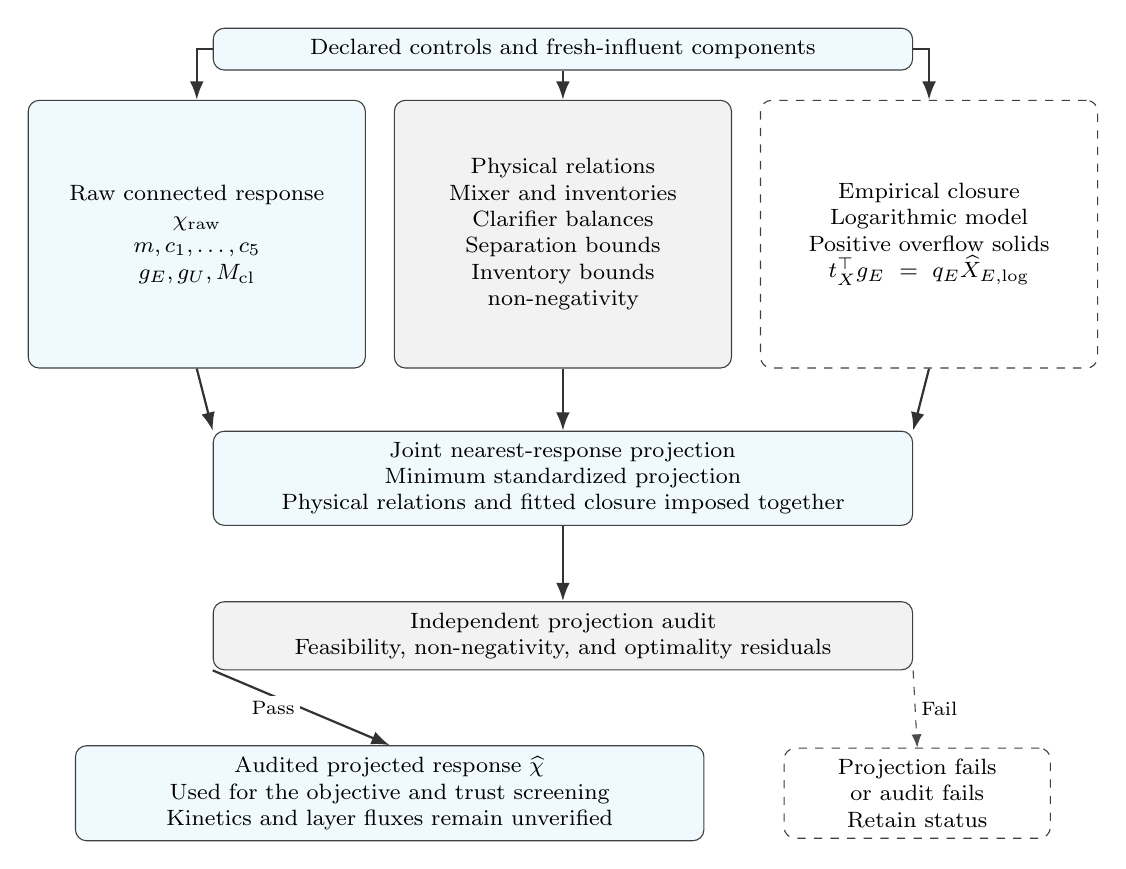
\begin{tikzpicture}[>=Latex,
block/.style={draw=black!75,rounded corners,fill=cyan!6,align=center,font=\footnotesize,inner sep=4pt},
physical/.style={block,fill=black!5},
empirical/.style={block,dashed,fill=white},
flow/.style={->,thick,draw=black!80},
failflow/.style={->,dashed,draw=black!70},
lab/.style={font=\scriptsize,fill=white,inner sep=2pt}]
\node[block,text width=8.6cm] (inputs) at (0,0) {Declared controls and fresh-influent components};
\node[block,text width=4.0cm,minimum height=3.4cm] (raw) at (-4.65,-2.35)
{Raw connected response\\$\chi_{\rm raw}$\\$m,c_1,\ldots,c_5$\\$g_E,g_U,M_{\rm cl}$};
\node[physical,text width=4.0cm,minimum height=3.4cm] (phys) at (0,-2.35)
{Physical relations\\Mixer and inventories\\Clarifier balances\\Separation bounds\\Inventory bounds\\non-negativity};
\node[empirical,text width=4.0cm,minimum height=3.4cm] (closure) at (4.65,-2.35)
{Empirical closure\\Logarithmic model\\Positive overflow solids\\$t_X^\top g_E=q_E\widehat X_{E,\log}$};
\node[block,text width=8.6cm] (projection) at (0,-5.45)
{Joint nearest-response projection\\Minimum standardized projection\\Physical relations and fitted closure imposed together};
\node[physical,text width=8.6cm] (audit) at (0,-7.45)
{Independent projection audit\\Feasibility, non-negativity, and optimality residuals};
\node[block,text width=7.7cm] (output) at (-2.2,-9.45)
{Audited projected response $\widehat\chi$\\Used for the objective and trust screening\\Kinetics and layer fluxes remain unverified};
\node[empirical,text width=3.1cm] (failure) at (4.5,-9.45)
{Projection fails\\or audit fails\\Retain status};
\draw[flow] (inputs.south)--(phys.north);
\draw[flow] (inputs.west)-|(raw.north);
\draw[flow] (inputs.east)-|(closure.north);
\draw[flow] (raw.south)--(projection.north west);
\draw[flow] (phys.south)--(projection.north);
\draw[flow] (closure.south)--(projection.north east);
\draw[flow] (projection)--(audit);
\draw[flow] (audit.south west)--(output.north) node[midway,left,lab] {Pass};
\draw[failflow] (audit.south east)--(failure.north) node[midway,right,lab] {Fail};
\end{tikzpicture}
\caption{Conceptual information flow in the connected projection. The dashed closure block denotes an empirically fitted relation rather than a physical identity. Projection corrects all response blocks jointly. An audited solution satisfies the imposed relations to their numerical tolerances, while original-model evaluation remains necessary for complete kinetic and settling verification.}
\label{fig:plant_projection_architecture}
\end{figure}

The projected response is therefore a constrained prediction, not a solved layer profile. Its smallest standardized projection is meaningful only for the stated response scales and feasible set. Keeping the empirical closure visible also explains why an original mechanistic target can lie outside that set.

\subsection{An independently auditable optimality certificate}

Consider a separate hypothetical two-component projection. The raw prediction is $(-2,9)$, its coordinate scales are $(1,2)$, and the required total fixed by mass conservation is 10. The physical-coordinate problem is
\begin{equation}
\min_{c_1,c_2}\ \frac12(c_1+2)^2+\frac18(c_2-9)^2,
\qquad c_1+c_2=10,\quad c_1\ge0,\quad c_2\ge0.
\end{equation}
The second coefficient is $1/(2\times2^2)$. A change of one physical unit in component 2 costs less than the same change in component 1 because its scale is larger.

First omit non-negativity and introduce an equality multiplier $\lambda$. Stationarity and the total fixed by mass conservation give
\begin{align}
c_1+2+\lambda&=0,\\
\tfrac14(c_2-9)+\lambda&=0,\\
c_1+c_2&=10.
\end{align}
The first two equations imply $c_1=-2-\lambda$ and $c_2=9-4\lambda$. Their sum gives $7-5\lambda=10$, so $\lambda=-0.6$ and $(c_1,c_2)=(-1.4,11.4)$. mass conservation alone leaves a negative component.

Now impose the active boundary $c_1=0$, which forces $c_2=10$. Use multiplier $\mu_1\ge0$ for $-c_1\le0$ and $\mu_2\ge0$ for $-c_2\le0$. The Lagrangian is the objective plus $\lambda(c_1+c_2-10)-\mu_1c_1-\mu_2c_2$. Since component 2 is positive, its inequality is inactive and $\mu_2=0$. Its stationarity equation gives $\lambda=-0.25$. Component 1 then gives $2-0.25-\mu_1=0$, so $\mu_1=1.75$. Both inequality multipliers are non-negative, and both products $\mu_jc_j$ vanish. These checks certify the boundary solution rather than merely declaring it plausible.

In standardized coordinates, $u=(2,0.5)^\top$. The same problem has
\begin{equation}
E=\begin{bmatrix}1&2\end{bmatrix},\quad e=3,\quad
G_u=\begin{bmatrix}-1&0\\0&-2\end{bmatrix},\quad
g=\begin{bmatrix}-2\\9\end{bmatrix}.
\end{equation}
The equality is $u_1+2u_2=3$. The inequality rows are the two physical non-negativity requirements after substitution. This example explains the standardized form before its use for the larger plant.

At fixed inputs, write the standardized problem as
\begin{equation}
\min_u\tfrac12u^\top u,\qquad Eu=e,\qquad G_uu\le g.
\label{eq:plant_standard_projection}
\end{equation}
Let $\lambda^=$ be unrestricted equality multipliers and $\lambda^\le\ge0$ inequality multipliers. The optimality conditions are primal feasibility, dual feasibility, stationarity, and complementarity,
\begin{align}
u+E^\top\lambda^=+G_u^\top\lambda^\le&=0,\\
\lambda^\le_j(g_j-(G_uu)_j)&=0\quad\text{for every }j.
\label{eq:plant_projection_optimality}
\end{align}
To derive the dual value, collect the linear terms in the Lagrangian. Define $v=E^\top\lambda^=+G_u^\top\lambda^\le$. Completing the square gives
\begin{align}
\tfrac12u^\top u+v^\top u-e^\top\lambda^=-g^\top\lambda^\le
&=\tfrac12\|u+v\|_2^2-\tfrac12\|v\|_2^2\\
&\quad-e^\top\lambda^=-g^\top\lambda^\le.
\end{align}
The first term has minimum zero at $u=-v$. Minimizing over $u$ therefore gives the dual value,
\begin{equation}
d(\lambda^=,\lambda^\le)=
-\tfrac12\|E^\top\lambda^=+G_u^\top\lambda^\le\|_2^2
-e^\top\lambda^=-g^\top\lambda^\le.
\end{equation}
For primal- and dual-feasible quantities, the gap is
\begin{equation}
\Gamma=\tfrac12\|u+E^\top\lambda^=+G_u^\top\lambda^\le\|_2^2
+(\lambda^\le)^\top(g-G_uu)\ge0.
\label{eq:plant_projection_gap}
\end{equation}
It vanishes exactly when stationarity and complementarity hold. This gives a mathematical certificate of the unique projection \citep{Boyd2004}. Numerical acceptance checks the individual residuals independently. A small reported gap does not replace a non-negativity or equality check.

The hypothetical two-component example permits every certificate number to be checked. With $\lambda^{=}=-0.25$ and $\lambda^\le=(1.75,0)^\top$,
\begin{align}
E^\top\lambda^=+G_u^\top\lambda^\le&=(-2,-0.5)^\top=-u,\\
g-G_uu&=(0,10)^\top,\\
\tfrac12u^\top u&=\tfrac12(4+0.25)=2.125,\\
d&=-2.125-3(-0.25)-[-2(1.75)]=2.125.
\end{align}
The primal and dual values agree. Stationarity is zero coordinate by coordinate, and the complementarity sum is $1.75(0)+0(10)=0$. The gap is consequently zero. A multiplier with the wrong sign would fail dual feasibility even if some other residual happened to be small.

Every distinct trial receives a projection solve from an independent initialization. An operator-splitting quadratic solver of the type studied by \citet{Stellato2020} supplies a numerical candidate. Multipliers are reconstructed independently through bounded-variable least squares for the audit. Numerical retries change the solver settings while preserving the mathematical problem.

\subsection{The conditional error guarantee}

Let $\mathcal C$ be the fixed-input feasible set and use the norm
$\|v\|_{D_\chi^{-1}}=\|D_\chi^{-1}v\|_2$. This norm has the scalar meaning
\begin{equation}
\|v\|_{D_\chi^{-1}}^2=\sum_{k=1}^{n_\chi}\frac{v_k^2}{s_k^2}.
\end{equation}
To see the error argument, temporarily work in standardized coordinates. Write $a_k=\chi_{{\rm raw},k}/s_k$, $q_k=\widehat\chi_k/s_k$, and $t_k=\chi_{{\rm ref},k}/s_k$. The transformed feasible set is convex because the scales define an invertible linear change of coordinates.

For any feasible comparison point $z$, the segment $q+\tau(z-q)$ remains feasible for $0\le\tau\le1$. The projection objective cannot decrease when leaving its minimizer along that segment. Its derivative at zero must therefore satisfy
\begin{equation}
\sum_k(q_k-a_k)(z_k-q_k)\ge0.
\end{equation}
When the reference itself is feasible, take $z=t$. Reversing both signs gives $\sum_k(a_k-q_k)(q_k-t_k)\ge0$. The componentwise identity
\begin{align}
(a_k-t_k)^2&=(a_k-q_k)^2+(q_k-t_k)^2\\
&\quad+2(a_k-q_k)(q_k-t_k)
\end{align}
then implies, after summing over coordinates,
\begin{equation}
\sum_k(q_k-t_k)^2\le\sum_k(a_k-t_k)^2-\sum_k(a_k-q_k)^2.
\end{equation}
The last sum is exactly the squared standardized projection. Returning to the physical-coordinate notation, if a mechanistic reference $\chi_{\rm ref}$ belongs exactly to $\mathcal C$, the projection variational inequality gives
\begin{equation}
\|\widehat\chi-\chi_{\rm ref}\|_{D_\chi^{-1}}^2
\le\|\chi_{\rm raw}-\chi_{\rm ref}\|_{D_\chi^{-1}}^2
-\|\widehat u\|_2^2.
\label{eq:plant_projection_error_exact}
\end{equation}
Thus the projection cannot increase aggregate squared error in this particular metric to an exactly feasible target. It does not guarantee improvement in every component, an unweighted physical-unit score, or the operating objective.

In the hypothetical weighted two-component problem, take the feasible reference $(3,7)$. Raw squared error is $(-2-3)^2+(9-7)^2/4=26$. Projected squared error is $(0-3)^2+(10-7)^2/4=11.25$. Projection size squared is $2^2+0.5^2=4.25$. The bound reads $11.25\le26-4.25=21.75$. The second component's absolute error increases from 2 to 3 even though the aggregate weighted error decreases. This is why the guarantee cannot be restated as improvement of every coordinate.

The fitted overflow equality usually differs from the mechanistic endpoint. A physically consistent mechanistic target can therefore lie outside $\mathcal C$. Define
\begin{equation}
\delta_{\rm feas}=\|P_{\mathcal C}(\chi_{\rm ref})-\chi_{\rm ref}\|_{D_\chi^{-1}}.
\end{equation}
Let $p$ be the closest feasible point to $t$ in standardized coordinates. The previous segment argument now applies to $z=p$. Split the remaining inner product into a feasible-point part and a reference-distance part,
\begin{align}
\sum_k(a_k-q_k)(q_k-t_k)
&=\sum_k(a_k-q_k)(q_k-p_k)\\
&\quad+\sum_k(a_k-q_k)(p_k-t_k).
\end{align}
The first term is non-negative. The magnitude of the second is at most
\begin{equation}
\left[\sum_k(a_k-q_k)^2\right]^{1/2}
\left[\sum_k(p_k-t_k)^2\right]^{1/2}
=r_{\rm corr}\delta_{\rm feas}.
\end{equation}
This is the scalar Cauchy--Schwarz inequality. It bounds how far an infeasible reference can weaken the projection argument. Let $r_{\rm corr}=\|\chi_{\rm raw}-P_{\mathcal C}(\chi_{\rm raw})\|_{D_\chi^{-1}}$. Apply the projection variational inequality with the feasible comparison point $P_{\mathcal C}(\chi_{\rm ref})$. Expanding the squared error and bounding the remaining inner product gives
\begin{align}
\|P_{\mathcal C}(\chi_{\rm raw})-\chi_{\rm ref}\|_{D_\chi^{-1}}^2
&\le\|\chi_{\rm raw}-\chi_{\rm ref}\|_{D_\chi^{-1}}^2
-r_{\rm corr}^2+2r_{\rm corr}\delta_{\rm feas}\\
&\le\|\chi_{\rm raw}-\chi_{\rm ref}\|_{D_\chi^{-1}}^2+\delta_{\rm feas}^2.
\end{align}
Taking square roots therefore gives the more easily interpreted bound
\begin{equation}
\|P_{\mathcal C}(\chi_{\rm raw})-\chi_{\rm ref}\|_{D_\chi^{-1}}
\le\|\chi_{\rm raw}-\chi_{\rm ref}\|_{D_\chi^{-1}}+\delta_{\rm feas}.
\label{eq:plant_projection_error_general}
\end{equation}
The distance includes any finite numerical infeasibility of the reference. The guarantee cannot be invoked by checking only the physical identities and ignoring the empirical equality. The weighted-projection discussion in \citet{SturmSilva2024} likewise separates mass conservation from predictive improvement. Biological kinetics, nonlinear settling, and dynamic stability remain outside the projected set.

For a hypothetical illustration of the empirical-closure issue, let the total fixed by mass conservation still be 10 but also require the first component to equal a fitted value of 4. The feasible set then contains only $(4,6)$. Suppose the mechanistic reference and raw prediction are both $(2,8)$ with scales $(1,2)$. They satisfy the physical total and non-negativity but do not satisfy the fitted equality. Raw error is zero. Projection introduces weighted error $\sqrt{(4-2)^2+(6-8)^2/4}=\sqrt5$. The reference distance to the set is also $\sqrt5$, so the general bound is met exactly. Physical identities alone would have given the wrong premise for the stronger guarantee.

\subsection{Control-dependent sensitivities}

With fixed constraint matrices and an affine parameter-dependent right-hand side, a parametric quadratic projection can have a piecewise affine solution \citep{Tondel2003}. That more restrictive setting is not assumed here. Hydraulic coefficients, inverse flow ratios, the input features, and the exponential endpoint all depend on $\vartheta$. The projected plant response is generally piecewise smooth where regularity holds. It need not be globally piecewise affine or differentiable at an active-set change.

The differentiation can first be seen in a scalar hypothetical projection,
\begin{equation}
\min_u\tfrac12u^2,\qquad b(\theta)u=e(\theta),
\end{equation}
where $\theta$ is one control and $b(\theta)\ne0$. Stationarity and feasibility are $u+b\lambda=0$ and $bu=e$. Written together, they form the two-by-two system
\begin{equation}
\begin{bmatrix}1&b\\b&0\end{bmatrix}
\begin{bmatrix}u\\\lambda\end{bmatrix}
=\begin{bmatrix}0\\e\end{bmatrix}.
\end{equation}
Differentiate the two scalar equations with respect to $\theta$. The product rule gives $u'+b'\lambda+b\lambda'=0$ and $b'u+bu'=e'$. Moving known products to the right leaves
\begin{equation}
\begin{bmatrix}1&b\\b&0\end{bmatrix}
\begin{bmatrix}u'\\\lambda'\end{bmatrix}
=\begin{bmatrix}-b'\lambda\\e'-b'u\end{bmatrix}.
\end{equation}
The matrix is unchanged. Its right-hand side now contains derivatives of both coefficients and targets.

For $b=1+\theta$ and $e=\theta$, the solution is $u=\theta/(1+\theta)$ and $\lambda=-\theta/(1+\theta)^2$. At the hypothetical control $\theta=1$, the values are $u=0.5$ and $\lambda=-0.25$. The derivative system becomes
\begin{equation}
\begin{bmatrix}1&2\\2&0\end{bmatrix}
\begin{bmatrix}u'\\\lambda'\end{bmatrix}
=\begin{bmatrix}0.25\\0.5\end{bmatrix}.
\end{equation}
Its second row gives $u'=0.25$ and its first gives $\lambda'=0$. Direct differentiation of $u=\theta/(1+\theta)$ gives the same $u'=1/(1+\theta)^2$. Ignoring $b'$ would instead differentiate a problem whose constraint coefficient did not vary.

For a stable active set, stack equality rows and active inequality rows into $B(\vartheta)$ and their right-hand sides into $b_a(\vartheta)$. The stationary system is
\begin{equation}
\begin{bmatrix}I&B^\top\\B&0\end{bmatrix}
\begin{bmatrix}u\\\lambda_a\end{bmatrix}
=\begin{bmatrix}0\\b_a\end{bmatrix}.
\label{eq:plant_active_system}
\end{equation}
The componentwise product rule is now applied to $u+B^\top\lambda_a=0$ and $Bu=b_a$,
\begin{align}
\partial_j u+B^\top\partial_j\lambda_a&=-(\partial_jB)^\top\lambda_a,\\
B\partial_j u&=\partial_jb_a-(\partial_jB)u.
\end{align}
For a control $\vartheta_j$, putting these derivative equations into one block system gives
\begin{equation}
\begin{bmatrix}I&B^\top\\B&0\end{bmatrix}
\begin{bmatrix}\partial_j u\\\partial_j\lambda_a\end{bmatrix}
=\begin{bmatrix}-(\partial_jB)^\top\lambda_a\\
\partial_jb_a-(\partial_jB)u\end{bmatrix}.
\label{eq:plant_active_sensitivity}
\end{equation}
Since $D_\chi$ is fixed after fitting, the physical response derivative is $\partial_j\widehat\chi=\partial_j\chi_{\rm raw}+D_\chi\partial_j\widehat u$. For the endpoint, first differentiate the scalar fitted logarithm, which gives $\partial_j(\widehat\beta^\top\phi)=\widehat\beta^\top\partial_j\phi$. Exponential differentiation then gives $\partial_j\widehat X_{E,\log}=\widehat X_{E,\log}\widehat\beta^\top\partial_j\phi$. Applying the product rule to its flow-weighted value gives the endpoint derivative,
\begin{equation}
\partial_j(q_E\widehat X_{E,\log})
=(\partial_jq_E)\widehat X_{E,\log}
+q_E\widehat X_{E,\log}\widehat\beta_{E,\gamma_E}^\top\partial_j\phi.
\end{equation}
Ignoring this term would differentiate a different optimization problem.

These derivatives are used only when active rows are independent, the stationary matrix is well conditioned, active inequality multipliers are strictly positive, and independent perturbation checks pass. Near degeneracy, different active descriptions can correspond to the same unique response. Uniqueness of the projection therefore does not ensure a reliable classical derivative. A value-only outer method remains available when the derivative chain cannot be validated.

\section{Treatment priorities, resource measures, and operating safeguards}

\subsection{A common engineering objective}

The effluent-quality map in Table~\ref{tab:component_basis_composites} gives
\begin{equation}
z_E=I_{\rm comp}c_E=\operatorname{col}(\mathrm{COD},\mathrm{TN},\mathrm{TP},\mathrm{TSS}).
\end{equation}
Let the four diagonal entries of $D_T$ be $T_{COD},T_{TN},T_{TP},T_{TSS}$. Dividing each effluent quantity by its own scale gives a dimensionless quality contribution. The scalar weighted sum is
\begin{equation}
\begin{aligned}
j_Q={}&\varpi_{Q,COD}\frac{z_{E,COD}}{T_{COD}}
+\varpi_{Q,TN}\frac{z_{E,TN}}{T_{TN}}\\
&+\varpi_{Q,TP}\frac{z_{E,TP}}{T_{TP}}
+\varpi_{Q,TSS}\frac{z_{E,TSS}}{T_{TSS}}.
\end{aligned}
\end{equation}
For positive fixed normalization $D_T$ and quality priorities $\varpi_Q\ge0$ with $\mathbf1^\top\varpi_Q=1$, this sum is written compactly as
\begin{equation}
j_Q=\varpi_Q^\top D_T^{-1}z_E.
\label{eq:plant_quality_objective}
\end{equation}
The four totals describe different treatment concerns. They do not identify which individual nutrient transformations occur. A nearly constant TN across a reactor can accompany conversion of ammonium to nitrite. A decrease in overflow TP can arise from particulate separation rather than an additional clarifier reaction. The nutrient-control guidance of \citet{USEPA2009} and component-resolved treatment framework of \citet{Zhang2026} support inspecting species and solids flows alongside aggregate quality measures.

Normalizing a bounded setting subtracts its lower bound and divides by the full range. This gives zero at the lower bound and one at the upper bound. For example, $H=18$ h within 6--36 h gives $(18-6)/(36-6)=0.4$. Aeration instead sums physical transfer capacities. Each product $V_i k_La_i$ has units m$^3$ d$^{-1}$, so its fixed reference has the same units. Wasted solids are proportional to $Q_0wX_U$. Dividing this rate by its fixed reference $Q_0w^UX_U^{\rm ref}$ cancels $Q_0$. The resource terms are
\begin{align}
j_H&=\frac{H-H^L}{H^U-H^L},\qquad
j_A=\frac{\sum_{i\in\mathcal A}V_i k_La_i}{E_A^{\rm ref}},\\
j_I&=\frac{r_I-r_I^L}{r_I^U-r_I^L},\qquad
j_R=\frac{r_R-r_R^L}{r_R^U-r_R^L},\\
j_W&=\frac{wX_U}{w^UX_U^{\rm ref}}.
\label{eq:plant_resource_objective}
\end{align}
The set $\mathcal A$ contains stages that can be aerated. The aeration reference $E_A^{\rm ref}>0$ is fixed before optimization. It is the maximum transfer-capacity numerator over the declared operating box. A fixed reference prevents an increase in selected volume from being canceled by a changing denominator.

The aeration proxy measures transfer capacity. Actual oxygen transfer also depends on the dissolved-oxygen deficit in Equation~\eqref{eq:plant_reactor}. The energy-management model of \citet{Miederer2025} distinguishes aeration and other energy demands. The treatment model of \citet{Zhang2026} makes the oxygen-transfer driving force explicit. The present dimensionless terms do not constitute a monetary cost calculation or a measurement of energy consumption.

Write the overall coefficients in the same order as the six terms. The complete scalar objective is
\begin{equation}
J=\varpi_1j_Q+\varpi_2j_H+\varpi_3j_A+\varpi_4j_I+\varpi_5j_R+\varpi_6j_W.
\end{equation}
Its compact vector form is
\begin{equation}
J(\vartheta,\chi,\varpi)=\varpi^\top
\operatorname{col}(j_Q,j_H,j_A,j_I,j_R,j_W),\qquad
\varpi\ge0,\quad\mathbf1^\top\varpi=1.
\label{eq:plant_engineering_objective}
\end{equation}
The overall vector $\varpi$ separates quality from capacity and resource priorities. The vector $\varpi_Q$ separates priorities among the quality measures. These coefficients are choices about trade-offs. They are not percentages of the objective attained at an operating point.

For the equal-volume case,
\begin{equation}
j_A=\frac{H}{36\ \mathrm{h}}\frac{a_3+a_4+a_5}{3}.
\label{eq:plant_aeration_proxy_example}
\end{equation}
This follows from $V_i=Q_0H/(24n_r)$ and $k_La_i=47a_i$. For hypothetical settings with all three aeration coordinates equal to one, reducing $H$ from 36 h to 12 h reduces this proxy from one to one-third. The normalized aeration settings have stayed the same, but the total transfer capacity has changed with volume. A comparison based only on the aeration coordinates would miss this effect.

The baseline priority vectors are
\begin{equation}
\varpi=(0.50,0.15,0.20,0.05,0.05,0.05)^\top,\qquad
\varpi_Q=\tfrac14\mathbf1_4.
\label{eq:plant_objective_priorities}
\end{equation}
Quality has the largest individual coefficient. Aeration has the largest resource coefficient. The importance of oxygen supply and solids age to treatment and energy use is discussed by \citet{Leu2012}. The exact coefficients remain case-study preferences. Changes in those preferences define separate operating questions and require separately reported decisions.

A hypothetical objective calculation can now be followed through all six terms. Use effluent values $(40,5,1,4)$ mg L$^{-1}$ and illustrative fixed quality scales $(100,10,2,20)$ mg L$^{-1}$. With equal quality priorities, $j_Q=(0.4+0.5+0.5+0.2)/4=0.4$. These illustrative scales are not estimated study quantities. Let $H=18$ h, $(a_3,a_4,a_5)=(0.8,0.6,0.4)$, $r_I=1$, $r_R=0.5$, $w=0.02$, and $X_U=6{,}000$ g m$^{-3}$.

The total biological volume is $Q_0H/24=7{,}500$ m$^3$, so each equal tank has volume 1{,}500 m$^3$. Aeration capacity is $1{,}500(47)(0.8+0.6+0.4)=126{,}900$ m$^3$ d$^{-1}$. Table~\ref{tab:plant_hypothetical_objective} gives every normalized term and weighted contribution. Their sum is 0.353. This arithmetic illustrates the declared objective and does not report a selected operating decision.

\begin{table}[htbp]
\centering\small
\caption{Hypothetical calculation of dimensionless objective contributions.}
\label{tab:plant_hypothetical_objective}
\begin{tabular}{llll}
\toprule Term & Calculation & Value & Weighted value\\\midrule
$j_Q$ & $(0.4+0.5+0.5+0.2)/4$ & 0.4 & 0.200\\
$j_H$ & $(18-6)/(36-6)$ & 0.4 & 0.060\\
$j_A$ & $126{,}900/423{,}000$ & 0.3 & 0.060\\
$j_I$ & $(1-0)/(4-0)$ & 0.25 & 0.0125\\
$j_R$ & $(0.5-0.25)/(1.25-0.25)$ & 0.25 & 0.0125\\
$j_W$ & $(0.02)(6{,}000)/[(0.05)(15{,}000)]$ & 0.16 & 0.008\\
\bottomrule
\end{tabular}
\end{table}

The overall priority of 0.50 for quality multiplies $j_Q$ after its four internal quality weights have been applied. A quality priority of one-quarter is therefore not an overall objective coefficient of one-quarter. Also, a resource reference need not be a hard maximum. In particular, $j_W$ can exceed one if its numerator exceeds the declared reference. A denominator used for normalization does not itself impose feasibility.

\subsection{Solids retention time and clarifier loading}

Stored solids and lost solids have different units. For two reactors, the stored mass would be $V_1X_1+V_2X_2+M_{\rm cl}$ in grams. Its loss rate would be $Q_EX_E+Q_0wX_U$ in grams per day. Dividing mass by mass per day gives days. The same accounting applies to all five reactors.

External solids leave in the overflow and waste-sludge streams,
\begin{equation}
\dot M_X=Q_0(q_EX_E+wX_U).
\label{eq:plant_external_solids_loss}
\end{equation}
Return sludge does not count as an external loss. With $X_i=t_X^\top c_i$, the whole-plant solids retention time is
\begin{equation}
\theta_X=\frac{\sum_{i=1}^{n_r}V_iX_i+M_{\rm cl}}{\dot M_X},
\qquad\dot M_X\ge\epsilon_X>0.
\label{eq:plant_solids_age}
\end{equation}
Its numerator includes the clarifier inventory. Omitting that mass would underestimate solids age for the same external loss rate. A wasting ratio alone also does not determine solids age because $wX_U$ and the stored mass both matter \citep{Alex2008}.

For a hypothetical accounting example, use $Q_0=10{,}000$ m$^3$ d$^{-1}$, $w=0.02$, $X_E=10$, and $X_U=6{,}000$ g m$^{-3}$. The two external loss contributions are
\begin{align}
Q_0q_EX_E&=10{,}000(0.98)(10)=98{,}000\ \mathrm{g\,d^{-1}},\\
Q_0wX_U&=10{,}000(0.02)(6{,}000)=1{,}200{,}000\ \mathrm{g\,d^{-1}}.
\end{align}
Their sum is 1{,}298{,}000 g d$^{-1}$. At a total reactor volume of 7{,}500 m$^3$, assigning every reactor 3{,}000 g TSS m$^{-3}$ gives 22{,}500{,}000 g in the reactors. If the clarifier inventory is 7{,}500{,}000 g, the total inventory is 30{,}000{,}000 g. The illustrative solids retention time is $30{,}000{,}000/1{,}298{,}000=23.11$ d. This ratio concerns the stated mass accounting and does not assert that these concentrations solve the mechanistic equations.

Clarifier surface loading divides the overflow volume rate by area. Clarifier solids loading divides the feed solids mass rate by area. Since one gram is $10^{-3}$ kilograms, its conversion appears before the area division. The descriptive clarifier loading measures are
\begin{equation}
\ell_{\rm surface}=\frac{Q_0q_E}{A_{\rm cl}},\qquad
\ell_{\rm solids}=\frac{10^{-3}Q_0q_CX_N}{A_{\rm cl}}.
\label{eq:plant_loading_measures}
\end{equation}
The factor $10^{-3}$ converts grams to kilograms. The surface quantity is in m d$^{-1}$ and the solids quantity is in kg m$^{-2}$ d$^{-1}$. These quantities and $\theta_X$ are descriptive measures in the baseline comparison. They are not additional optimization limits.

For the same hypothetical flow with $r_R=0.5$, $q_C=1.5$, $A_{\rm cl}=1{,}500$ m$^2$, and $X_N=3{,}000$ g m$^{-3}$, the surface loading is $9{,}800/1{,}500=6.53$ m d$^{-1}$. The feed solids rate is $10{,}000(1.5)(3{,}000)=45{,}000{,}000$ g d$^{-1}$, or 45{,}000 kg d$^{-1}$. Dividing by area gives 30 kg m$^{-2}$ d$^{-1}$. Using underflow instead of clarifier-feed solids in this formula would calculate a different loading quantity.

The common engineering safeguards are
\begin{equation}
X_U\le X_U^{\max},\qquad X_N\ge X_F^{\min}>0,\qquad
\dot M_X\ge\epsilon_X>0.
\label{eq:plant_engineering_safeguards}
\end{equation}
The positive feed-solids limit keeps particulate outlet reconstruction defined. The positive external-loss limit keeps solids retention time defined. The underflow bound represents the admitted thickening or solids-handling range. Their numerical values are plant-specific problem inputs selected before search. An underflow limit should be based on accepted sludge-handling conditions. The feed and loss floors should prevent undefined calculations without excluding physically relevant low-solids operation. These engineering inputs are distinct from the fixed $X_U^{\rm ref}=15{,}000$ g m$^{-3}$ used only to normalize the wasted-solids objective.

\subsection{Trust diagnostics without a mechanistic-accuracy guarantee}

The imposed physical balances alone admit states that do not satisfy all mechanistic equations. The empirical closure can also exclude mechanistic states. An optimizer might exploit an admitted response that does not solve the full kinetics or settling equations. The projection diagnostic first squares each standardized movement, averages these squares over the response coordinates, and takes the square root. For the hypothetical two-component projection $u=(2,0.5)$, it is $\sqrt{(4+0.25)/2}=1.458$. Dividing by the number of coordinates makes its interpretation comparable across response dimensions.

Feature leverage uses the feature vector and the regularized fitting geometry. In a hypothetical intercept-plus-one-feature example with three standardized feature values $(-\sqrt{3/2},0,\sqrt{3/2})$ and $\gamma=1$,
\begin{equation}
\Phi^\top\Phi+3\gamma R_\phi=
\begin{bmatrix}3&0\\0&6\end{bmatrix}.
\end{equation}
Its inverse is $\operatorname{diag}(1/3,1/6)$. At query feature $(1,z)$, leverage is $1/3+z^2/6$. It is $1/3$ at the center, $1/2$ at $z=1$, and $11/6$ at $z=3$. The largest development value in this teaching example is $7/12$. These numbers illustrate weaker joint feature support away from the observed range. They do not supply the plant's calibrated threshold.

The split diagnostic compares each particulate underflow flow with the flow expected from a common recovery factor. In a hypothetical two-particulate example with unit TSS weights, let the feed component concentrations be $(40,60)$, so $X_N=100$. An underflow component-flow vector $(20,30)$ has total 50 and gives numerators $100(20)-50(40)=0$ and $100(30)-50(60)=0$. Changing the outlet allocation to $(25,25)$ preserves total underflow solids but gives numerators 500 and $-500$. With illustrative fixed split scales of 500, the standardized values are 1 and $-1$, and their root mean square is one. Total solids consistency therefore need not establish composition consistency.

The reactor diagnostic first evaluates the kinetic balances, then divides each residual by its fixed balance scale, and finally computes their root mean square. In the hypothetical two-component reactor, a projected state $(9,6)$ preserves the upstream total of $(12,3)$. With $d=2$ and the reaction rate held at 8 for this illustration, its two residuals are $2(12-9)-8=-2$ and $2(3-6)+8=2$. A balance scale of 10 for each component gives standardized residuals $(-0.2,0.2)$ and a diagnostic of 0.2. The invariant is satisfied even though the kinetic equations are not.

These four fixed diagnostics are written compactly as
\begin{align}
\kappa_{\rm corr}&=\frac{\|D_\chi^{-1}(\widehat\chi-\chi_{\rm raw})\|_2}{\sqrt{n_\chi}},\\
\kappa_{\rm lev}&=\phi^\top(\Phi^\top\Phi+n_{\rm dev}\gamma R_\phi)^{-1}\phi,\\
\kappa_{\rm split}&=\left[\frac1{F_X}\sum_{f\in X}
\left\{\frac{X_Ng_{U,f}-(t_X^\top g_U)c_{n_r,f}}{d_{{\rm split},f}}\right\}^2\right]^{1/2},\\
\kappa_{\rm reac}&=\frac{\|D_{\rm bal}^{-1}f_{{\rm sm},\rm reactor}(\vartheta,\widehat\chi)\|_2}{\sqrt{n_rF}}.
\label{eq:plant_trust_diagnostics}
\end{align}
The first measures standardized projection size. A large value identifies a raw response that requires a large movement to satisfy the imposed constraints. It does not establish that the projected response is inaccurate. The projection is constrained and reported separately from the engineering objective.

The second diagnostic is regularized feature leverage. It measures input support within the fitted quadratic feature map. \citet{Sahigara2012} compare applicability-domain assessments and motivate checking where a statistical model is being used. Feature leverage does not detect every form of response error. A control vector inside its coordinate bounds may still have weak support in the joint feature space.

The third diagnostic checks the common particulate-recovery assumption in Equation~\eqref{eq:plant_outlet_reconstruction}. If every particulate component has the same recovery, its numerator vanishes. The projection enforces component mass conservation and densification but does not enforce that composition exactly. This diagnostic therefore checks a relation that can hold in the reduced mechanistic mapping while remaining outside the projection equalities.

The fourth diagnostic checks smooth reactor kinetics at the projected concentrations. It includes hydraulic transport, net biological conversion, and oxygen transfer on separate scales. It cannot supply a clarifier-layer residual because the surrogate has no internal layer concentrations. Its smoothing width is $10^{-8}$ under the definitions given below.

A row scale is based on the sizes of its separate physical terms before cancellation. Suppose a hypothetical row has terms $(100,-100)$ in one development state and $(200,-200)$ in another. Its net balance is zero in both states, but its terms have substantial magnitude. Their mean squared magnitude is $(100^2+100^2+200^2+200^2)/4=25{,}000$, giving a root mean square of 158.11. Scaling only the canceled net balance would lose this information. For a constraint row with $p$ terms $b_{ij}$ over $n_{\rm dev}$ development states, its fixed scale is
\begin{equation}
d_b=\max\left\{1,\left[\frac1{n_{\rm dev}p}
\sum_{i=1}^{n_{\rm dev}}\sum_{j=1}^{p}b_{ij}^2\right]^{1/2}\right\}.
\label{eq:plant_term_scales}
\end{equation}
The same convention defines inequality and split scales. The overflow row uses the mechanistic overflow flow and the out-of-fold fitted endpoint flow as its two terms. The floor of one is in the corresponding numerical row units. It is not a concentration floor.

Projection, split, and reactor limits use nearest-rank 95th percentiles of grouped out-of-fold development diagnostics. If sorted values are $v_{(1)},\ldots,v_{(n_{\rm dev})}$, the limit is $v_{(\lceil0.95n_{\rm dev}\rceil)}$. The leverage limit is the maximum development leverage under the final fitted feature map. These quantities are fixed before optimization. They are empirical guardrails rather than confidence bounds. A diagnostic with zero limit remains constrained to zero and uses one only as a numerical row scale.

The surrogate decision problem is consequently
\begin{equation}
\begin{aligned}
\min_{\vartheta}\quad&J(\vartheta,\widehat\chi(\vartheta,c_{\rm in}),\varpi),\\
\text{subject to}\quad&\vartheta\in\mathcal V,\\
&g_{\rm eng}(\vartheta,\widehat\chi)\le0,\\
&g_{\rm trust}(\vartheta,\chi_{\rm raw},\widehat\chi)\le0,\\
&\widehat\chi\text{ satisfies Equation~\eqref{eq:plant_joint_projection}}.
\end{aligned}
\label{eq:plant_surrogate_optimization}
\end{equation}
The lower problem is a convex quadratic projection. The upper problem is generally nonconvex. This distinction follows the nested-problem perspective described by \citet{Colson2007}. A best retained feasible candidate is not a certified global optimum. The trust-region analysis of \citet{Alexandrov1998} explains why reliable approximation management needs more than a small average prediction error. The four fixed diagnostics here do not establish the fully linear approximation conditions of a convergent adaptive trust-region method.


\section{Bounded products and the limits of a convex relaxation}

Flow and concentration products help explain why process optimization remains nonlinear even when a surrogate is linear in its fitted coefficients. A bounded product provides a simple example. Let $x_L\leq x\leq x_U$, $y_L\leq y\leq y_U$, and let $z$ represent the product $xy$. The four products
\[
(x-x_L)(y-y_L),\quad (x_U-x)(y_U-y),\quad
(x_U-x)(y-y_L),\quad (x-x_L)(y_U-y)
\]
are non-negative. Expanding the first gives $xy-x_Ly-y_Lx+x_Ly_L\geq0$. Replacing $xy$ by $z$ gives one lower bound on $z$. Expanding the other three products gives the remaining bounds. Together they form the McCormick relaxation \citep{McCormick1976}
\begin{equation}
\begin{aligned}
z&\geq x_Ly+y_Lx-x_Ly_L,\\
z&\geq x_Uy+y_Ux-x_Uy_U,\\
z&\leq x_Uy+y_Lx-x_Uy_L,\\
z&\leq x_Ly+y_Ux-x_Ly_U.
\end{aligned}
\label{eq:teaching_mccormick_relaxation}
\end{equation}
The four inequalities are linear in the variables $x$, $y$, and $z$. Every exact product within the stated bounds satisfies them. Their intersection nevertheless permits points that do not satisfy $z=xy$.

For a hypothetical pair with $0\leq x,y\leq1$, the bounds become $z\geq0$, $z\geq x+y-1$, $z\leq x$, and $z\leq y$. At $x=y=0.5$, they permit $0\leq z\leq0.5$. The exact product is only $z=0.25$. A favorable objective obtained at another permitted value of $z$ is therefore not, by itself, an attainable process response. Tighter variable bounds can improve the relaxation, but they do not generally replace the exact product relation. Process-network optimization uses this distinction when constructing bounds and assessing solutions \citep{RubioCastro2010,YangNetwork2014}.

This example separates a convex relaxation from the physical projection used here. The relaxation enlarges a nonlinear feasible set to obtain an optimization bound. The projection selects a response satisfying the declared mass conservation and non-negativity conditions near a predicted response. Neither operation alone proves that a control vector is a global optimum of the full mechanistic plant. The present fixed-configuration plant retains the surrogate-assisted and direct mechanistic searches described below. It does not substitute a mixed-integer network-design formulation for those searches.

\section{A direct mechanistic comparator}

\subsection{The full-state constrained optimization problem}

The direct route retains the controls and full reduced mechanistic state. It reconstructs $\chi(\vartheta,c_{\rm in},y)$ and evaluates the same engineering objective. Its finite-volume clarifier equations require a positive feed-solids denominator at solver iterates. An auxiliary variable $\widetilde X_F\ge X_F^{\min}$ supplies that denominator, with equality $\widetilde X_F=t_X^\top c_{n_r}$ imposed at feasibility.

In a hypothetical one-reactor, two-component, three-layer illustration, the full state is $(c_S,c_X,s_1,s_2,s_3)$. It has five entries rather than the nine entries of the reduced statistical response. A simple conversion rate $kc_S$ gives two reactor equations,
\begin{align}
0&=d(m_S-c_S)-kc_S,\\
0&=d(m_X-c_X)+kc_S.
\end{align}
The three layer equations are those obtained from the interface-flow balances above, divided by their own volumes. The direct problem imposes all five equations rather than replacing the two reactor equations by only their sum fixed by mass conservation. Its three-layer envelope contains two scalar inequalities, $s_1-s_2\le0$ and $s_2-s_3\le0$. Four layers would require $(s_1-s_2,s_1-s_3,s_2-s_4,s_3-s_4)\le0$. This ordering explains how the envelope is assembled for ten layers.

The auxiliary denominator also has a concrete role. An infeasible trial can have zero feed solids while a nonzero layer concentration is being adjusted. Division by the actual feed value would then be undefined. An independently bounded $\widetilde X_F$ keeps the trial calculation defined. The equality $\widetilde X_F=X_N$ must subsequently hold, so this device does not allow a zero-feed trial to be accepted as a feasible physical state. It provides a usable calculation during the search, not an alternative physical feed concentration.

Let $f_{\rm sm}$ collect all $n_rF$ reactor equations and all $L$ smoothed layer equations. Let
\begin{equation}
g_{\rm env}(y)=\operatorname{col}
(s_1\mathbf1_{L-2}-s_{2:L-1},\ s_{2:L-1}-s_L\mathbf1_{L-2}).
\end{equation}
The direct nonlinear program is
\begin{equation}
\begin{aligned}
\min_{\vartheta,y,\widetilde X_F}\quad&J(\vartheta,\chi(\vartheta,c_{\rm in},y,\widetilde X_F),\varpi),\\
\text{subject to}\quad&f_{\rm sm}(\vartheta,c_{\rm in},y,\widetilde X_F)=0,\\
&\widetilde X_F=t_X^\top c_{n_r},\quad\widetilde X_F\ge X_F^{\min},\\
&\vartheta\in\mathcal V,\quad y\ge0,\quad g_{\rm env}(y)\le0,\\
&g_{{\rm eng},\rm red}(\vartheta,\chi)\le0.
\end{aligned}
\label{eq:plant_direct_optimization}
\end{equation}
The reduced engineering vector removes the feed-solids row already imposed by the auxiliary equality and lower bound. The auxiliary does not alter a feasible physical state. It keeps the outlet mapping defined while a nonlinear solver moves through infeasible trial states.

\subsection{Smooth switches and continuation}

The exact kinetic and settling functions contain minima, maxima, positive parts, possible zero denominators, and a receiver switch. Derivative-based optimization benefits from smooth approximations to these operations. The chemical-process optimization treatment of \citet{BuzziFerraris2013} provides the general derivative and conditioning context. The exact identities
\begin{equation}
\max(a,b)=\frac{a+b+|a-b|}{2},\qquad
\min(a,b)=\frac{a+b-|a-b|}{2}
\end{equation}
show where the nondifferentiable absolute value enters. Replacing $|r|$ by $\sqrt{r^2+\delta^2}$ removes its corner for every $\delta>0$. The positive part uses the same replacement in $(v+|v|)/2$. A denominator regularization instead replaces $1/b$ by $b/(b^2+\delta^2)$. These are different operations chosen for different numerical difficulties. For positive width $\delta=\epsilon S$, define
\begin{align}
\max_\delta(a,b)&=\tfrac12\left[a+b+\sqrt{(a-b)^2+\delta^2}\right],\\
\min_\delta(a,b)&=\tfrac12\left[a+b-\sqrt{(a-b)^2+\delta^2}\right],\\
[v]_{+,\delta}&=\tfrac12\left[v+\sqrt{v^2+\delta^2}\right],\\
\left(\frac ab\right)_\delta&=\frac{ab}{b^2+\delta^2}.
\label{eq:plant_smooth_operations}
\end{align}
For negative $v$, the positive-part expression is evaluated as $\delta^2/[2(\sqrt{v^2+\delta^2}-v)]$ to avoid subtraction of nearly equal values. These approximations change the equations near a switch. They do not make the exact and smooth models equivalent.

For hypothetical values $a=2$, $b=1$, and $\delta=0.1$, the smooth maximum is $(3+\sqrt{1.01})/2=2.00249$ and the smooth minimum is 0.99751. The exact values are 2 and 1. For $v=-0.2$, the smooth positive part is $(-0.2+\sqrt{0.05})/2=0.01180$, while the exact positive part is zero. At $b=0$, the regularized quotient $ab/(b^2+\delta^2)$ is defined and equals zero. At $a=1$ and $b=0.1$, it is 5 for $\delta=0.1$, compared with the exact quotient 10. These differences illustrate why smaller widths and an independent exact-model evaluation are needed.

The stable positive-part expression follows by rationalization,
\begin{align}
\frac{v+\sqrt{v^2+\delta^2}}2
&=\frac{(v+\sqrt{v^2+\delta^2})(\sqrt{v^2+\delta^2}-v)}
{2(\sqrt{v^2+\delta^2}-v)}\\
&=\frac{\delta^2}{2(\sqrt{v^2+\delta^2}-v)}.
\end{align}
The numerator becomes $v^2+\delta^2-v^2=\delta^2$. This form avoids canceling a negative $v$ against a nearly equal square root.

For the receiver switch, first measure where the receiver concentration lies across its transition band. Subtracting the lower edge $X_t-h$ and dividing by the band width $2h$ maps that band to $[0,1]$. For receiver concentration $s$, the smooth switch is zero below $X_t-h$, one above $X_t+h$, and
\begin{equation}
6\zeta^5-15\zeta^4+10\zeta^3,\qquad
\zeta=\frac{s-X_t+h}{2h}
\label{eq:plant_receiver_switch}
\end{equation}
within the transition band. This polynomial matches the values and first two derivatives at the band endpoints. It gives smooth interpolation between the two gravitational-flux rules.

For the illustrative band $X_t=3{,}000$ and $h=10$ g m$^{-3}$, concentrations 2{,}990, 3{,}000, and 3{,}010 correspond to $\zeta=0,0.5,1$. The switch values are 0, 0.5, and 1. At 2{,}995, $\zeta=0.25$ and the switch is 0.10352. At 3{,}005, it is 0.89648. If the unrestricted gravitational flux is $J_1$ and the receiver-limited flux is $J_2$, interpolation gives $(1-\sigma)J_1+\sigma J_2$ for switch value $\sigma$. The switch therefore changes a flux rule gradually rather than only replacing a reported concentration.

Each argument scale $S$ is its development-set root mean square with a floor of one. Reactor arguments are pooled across stages. They include total oxidized nitrogen, fermentable substrate plus acetate, the hydrolysis denominator, the polyphosphate and stored-carbon denominators, and remaining storage capacity. Clarifier arguments include $s-f_{\rm ns}X_N$ and gravitational solids flux. The velocity scale is 250 m d$^{-1}$. These scales stay fixed throughout continuation.

The direct route reduces smoothing through three stages,
\begin{equation}
(\epsilon,h)=(10^{-6},10),\ (10^{-7},3),\ (10^{-8},1),
\label{eq:plant_continuation_sequence}
\end{equation}
where $h$ is in g TSS m$^{-3}$. Each stage initializes from the preceding stage. Continuation helps a solver approach sharper switches while preserving a usable starting state. The final smooth candidate still requires an exact-model evaluation.

\subsection{Jacobian structure and globalization}

The Jacobian entry $J_{jk}$ is the partial derivative of residual $f_j$ with respect to state coordinate $y_k$. It describes how one balance changes when one coordinate changes while the others are held fixed. For a hypothetical two-reactor soluble conversion with rate $kc_{i,S}$, soluble pass-through in the recycle gives
\begin{equation}
m_S=\frac{c_{{\rm in},S}+(r_I+r_R)c_{2,S}}{q_P}.
\end{equation}
The two soluble residuals are $f_{1,S}=d_1(m_S-c_{1,S})-kc_{1,S}$ and $f_{2,S}=d_2(c_{1,S}-c_{2,S})-kc_{2,S}$. Their two-by-two state block is
\begin{equation}
\frac{\partial(f_{1,S},f_{2,S})}{\partial(c_{1,S},c_{2,S})}
=\begin{bmatrix}
-(d_1+k)&d_1(r_I+r_R)/q_P\\
d_2&-(d_2+k)
\end{bmatrix}.
\end{equation}
The off-diagonal upper-right entry is created by recycle. Dropping it would treat the mixer as independent of the final reactor. For hypothetical values $d_1=d_2=2$, $k=1$, $r_I=1$, $r_R=0.5$, and $q_P=2.5$, the block is $\begin{bmatrix}-3&1.2\\2&-3\end{bmatrix}$. Its entries have units d$^{-1}$ because the residual has concentration-per-day units and its derivative is with respect to concentration.

Finite differences permit an independent check of those entries. Increasing $c_{1,S}$ by 0.01 g m$^{-3}$ changes $f_{1,S}$ by $-0.03$ g m$^{-3}$ d$^{-1}$, giving $-0.03/0.01=-3$. Increasing $c_{2,S}$ by the same amount changes $m_S$ by 0.006 and $f_{1,S}$ by 0.012, giving 1.2. These values are exact for the hypothetical linear teaching equations. In a nonlinear residual, the check instead uses a small step $h$,
\begin{equation}
J_{jk}\approx\frac{f_j(y+he_k)-f_j(y-he_k)}{2h}.
\end{equation}
Here $e_k$ changes only coordinate $k$. Near a non-negative boundary, a central step can leave the allowed state region. A second-order forward alternative is
\begin{equation}
J_{jk}\approx\frac{-3f_j(y)+4f_j(y+he_k)-f_j(y+2he_k)}{2h}.
\end{equation}
The step has the physical unit of $y_k$. Scaling coordinates makes its relative size comparable across different component bases.

For three layers at fixed feed conditions, only neighboring concentrations enter each interface flux. Their layer Jacobian therefore has the pattern
\begin{equation}
J_{\rm layer}=\begin{bmatrix}\star&\star&0\\\star&\star&\star\\0&\star&\star\end{bmatrix},
\end{equation}
where a star denotes an entry that may be nonzero. Feed solids and outlet reconstruction add connections to reactor coordinates. The zeros describe the declared dependency structure and are not approximations made to reduce computation.

The direct residual is sparse in its mechanistic state. A reactor balance depends on its own component vector and the preceding stage. Recycle reconstruction adds dependencies on final-reactor and underflow quantities. A layer balance depends on nearby layer concentrations, feed solids, and hydraulic controls. The inventory and reporting maps are linear aggregations. These dependencies provide a structured Jacobian rather than a dense arbitrary response map.

Scaling is applied before testing Jacobian conditioning or comparing residual sizes. Different component bases include oxygen, COD, nitrogen, phosphorus, solids, and charge equivalents. An unscaled norm could be dominated by a large solids balance and conceal a nutrient-balance defect. Analytic derivatives or differentiated smooth equations supply the optimization Jacobian. Independent finite differences are retained for derivative checks. Sparse linear algebra exploits the local reactor and layer connections without omitting recycle terms.

The direct search uses the interior-point filter method studied by \citet{WachterBiegler2006}. Its line search manages progress in objective and constraint violation. This numerical globalization controls acceptance of local steps. It does not make a nonconvex plant objective globally convex or establish a global optimum. The surrogate route similarly separates numerical search progress from the final feasibility and stationarity audits.

\section{Case-study domain and fixed parameters}

\subsection{Topology and free controls}

The case study has five equal-volume reactors and ten clarifier layers. Reactors 1 and 2 are unaerated. Reactors 3--5 have independent aeration controls. The free-control vector is
\begin{equation}
\vartheta=(H,a_3,a_4,a_5,r_I,r_R,w)^\top\in\mathbb R^7.
\label{eq:plant_case_controls}
\end{equation}
For every stage, $h_i=H/5$. The unaerated settings are $a_1=a_2=0$, the aerated transfer coefficients are $k_La_i=47a_i$ d$^{-1}$, and $\xi_i=0$. These are case-study conditions rather than structural restrictions on the connected formulation.

\begin{table}[htbp]
\centering\small
\caption{Plant geometry and operating domain.}
\label{tab:plant_operating_domain}
\begin{tabular}{p{0.47\linewidth}p{0.40\linewidth}}
\toprule
Quantity & Value or interval\\
\midrule
Fresh-influent flow $Q_0$ & 10{,}000 m$^3$ d$^{-1}$\\
Reactors $n_r$, layers $L$, feed layer $\ell_F$ & 5, 10, 5\\
Reactor volume fraction $f_i^V$ & $1/5$ for every stage\\
Clarifier area and total depth & 1{,}500 m$^2$ and 4.0 m\\
Clarifier total and individual layer volumes & 6{,}000 m$^3$ and 600 m$^3$\\
Nominal total HRT $H$ & 6--36 h\\
Each of $a_3,a_4,a_5$ & 0--1 independently\\
Mixed-liquor recycle $r_I$ & 0--4\\
Return-sludge ratio $r_R$ & 0.25--1.25\\
Waste-sludge ratio $w$ & 0.001--0.05\\
Aeration reference $E_A^{\rm ref}$ & 423{,}000 m$^3$ d$^{-1}$\\
Wasted-solids reference $X_U^{\rm ref}$ & 15{,}000 g TSS m$^{-3}$\\
\bottomrule
\end{tabular}
\end{table}

The equal volumes provide a compact unaerated-to-aerated train. The layer depth is 0.4 m. The operating intervals preserve both positive clarifier outlet flow ratios. Together with 20 influent coordinates, the seven controls give 27 statistical inputs, 406 features, and 161 reduced-response coordinates. The mechanistic state has 110 coordinates. The projection has 76 equality rows and 12 physical inequality rows. Adding response non-negativity gives 173 inequality rows.

Changing the number of reactors or free controls changes the statistical dimensions. Changing the layer count changes the mechanistic dimension and inventory mapping but does not add coordinates to the aggregate surrogate response. In either case, physical and predictive validation must be repeated. A small aggregate response does not establish insensitivity to the clarifier discretization.

\subsection{Fresh-influent intervals}

Table~\ref{tab:plant_influent_intervals} defines independent intervals for the plant experiment. The nominal influent is their componentwise midpoint. The concentration bases and quality-map weights are those in Table~\ref{tab:component_basis_composites}. The plant alkalinity interval is 1.6--5.2 mol charge equivalents m$^{-3}$. It belongs to this connected-plant design and is not interchangeable with an interval specified for an isolated-reactor experiment.

\begin{table}[htbp]
\centering\small
\caption{Independent fresh-influent intervals for the connected plant.}\label{tab:plant_influent_intervals}
\begin{tabular}{lrrl}
\toprule
Component & Lower & Upper & Constituent basis\\
\midrule
$S_O$ & 0 & 0.5 & oxygen\\
$S_F$ & 20 & 180 & COD\\
$S_A$ & 5 & 80 & COD\\
$S_{NH4}$ & 12 & 55 & nitrogen\\
$S_{NO2}$ & 0 & 3 & nitrogen\\
$S_{NO3}$ & 0 & 8 & nitrogen\\
$S_{N2}$ & 0 & 2 & nitrogen\\
$S_{PO4}$ & 2 & 18 & phosphorus\\
$S_I$ & 10 & 90 & COD\\
$S_{ALK}$ & 1.6 & 5.2 & charge equivalents\\
$X_I$ & 20 & 120 & COD\\
$X_S$ & 60 & 280 & COD\\
$X_H$ & 15 & 100 & COD\\
$X_{PAO}$ & 5 & 60 & COD\\
$X_{PP}$ & 2 & 20 & phosphorus\\
$X_{PHA}$ & 1 & 30 & COD\\
$X_{AOB}$ & 0.5 & 8 & COD\\
$X_{NOB}$ & 0.5 & 8 & COD\\
$X_{MeP}$ & 0 & 12 & solids\\
$X_{MeOH}$ & 0 & 12 & solids\\
\bottomrule
\end{tabular}
\end{table}

All concentration values are in grams of the stated constituent per m$^3$, apart from alkalinity. Numerically, g m$^{-3}$ equals mg L$^{-1}$. Independent interval sampling is an experimental design. It does not assert that all sampled influent combinations occur with equal frequency at a real plant.

\subsection{Stoichiometric, kinetic, and settling parameters}

The constants in Tables~\ref{tab:plant_stoichiometric_constants}--\ref{tab:plant_settling_constants} define the plant case. They are fixed parameters rather than fitted kinetic estimates. A parameter's concentration basis follows the associated component. Symbols with several process subscripts on the same row have equal values. The two nitrifier populations remain separate, with different growth rates and oxygen half-saturation constants.

\begin{table}[htbp]
\centering\small
\caption{Fixed yields, constituent contents, and conversion factors.}\label{tab:plant_stoichiometric_constants}
\begin{tabular}{p{0.38\linewidth}p{0.13\linewidth}p{0.38\linewidth}}
\toprule Parameter & Value & Unit or interpretation\\\midrule
$Y_H,Y_{PAO}$ & 0.625 & g biomass COD per g substrate COD\\
$Y_{PHA}$ & 0.20 & g stored COD per g phosphorus\\
$Y_{PO4}$ & 0.40 & g phosphorus per g stored COD\\
$Y_{AOB}$ & 0.18 & g biomass COD per g nitrogen\\
$Y_{NOB}$ & 0.08 & g biomass COD per g nitrogen\\
$f_{SI}$ & 0 & soluble inert fraction\\
$f_{XI}$ & 0.10 & particulate inert fraction\\
$i_{N,SI}$ & 0.01 & g nitrogen per g COD\\
$i_{N,SF},i_{N,XS}$ & 0 & g nitrogen per g COD\\
$i_{N,XI}$ & 0.02 & g nitrogen per g COD\\
$i_{N,BM}$ & 0.07 & g nitrogen per g biomass COD\\
$i_{P,SI},i_{P,SF},i_{P,XS}$ & 0 & g phosphorus per g COD\\
$i_{P,XI}$ & 0.01 & g phosphorus per g COD\\
$i_{P,BM}$ & 0.02 & g phosphorus per g biomass COD\\
$i_{P,MeP}$ & $1/4.87$ & g phosphorus per g metal-phosphate solids\\
$\gamma_{OH}$ & 3.45 & g metal-hydroxide solids per g phosphorus\\
\bottomrule
\end{tabular}
\end{table}

\begin{table}[htbp]
\centering\small
\caption{Fixed hydrolysis and heterotrophic rate and saturation constants.}
\label{tab:plant_kinetic_constants}
\begin{tabular}{p{0.48\linewidth}p{0.10\linewidth}p{0.31\linewidth}}
\toprule Parameter & Value & Unit\\\midrule
$K_H$ & 3.0 & d$^{-1}$\\
$\eta_{{\rm hyd},NO3},\eta_{{\rm hyd},NO2}$ & 0.6 & dimensionless\\
$\eta_{{\rm hyd},fe}$ & 0.4 & dimensionless\\
$K_{O,\rm hyd},K_{O,H},K_{O,PAO}$ & 0.20 & g oxygen m$^{-3}$\\
$K_{NO3,\rm hyd},K_{NO2,\rm hyd},K_{NOx,\rm hyd}$ & 0.5 & g nitrogen m$^{-3}$\\
$K_X$ & 0.10 & g substrate COD per g biomass COD\\
$\mu_H$ & 6.0 & d$^{-1}$\\
$q_{fe}$ & 3.0 & d$^{-1}$\\
$b_H$ & 0.40 & d$^{-1}$\\
$\eta_{H,NO3},\eta_{H,NO2}$ & 0.9 & dimensionless\\
$K_F,K_{fe},K_A$ & 4.0 & g COD m$^{-3}$\\
$K_{NO3,H},K_{NO2,H},K_{NOx,H}$ & 0.5 & g nitrogen m$^{-3}$\\
$K_{NH4,H},K_{NH4,PAO},K_{NH4,NOB}$ & 0.05 & g nitrogen m$^{-3}$\\
$K_{PO4,H},K_{PO4,PAO},K_{PO4,\rm nit}$ & 0.01 & g phosphorus m$^{-3}$\\
$K_{ALK,H},K_{ALK,PAO}$ & 0.10 & mol equivalents m$^{-3}$\\
\bottomrule
\end{tabular}
\end{table}

\begin{table}[htbp]
\centering\small
\caption{Fixed storage, nitrifier, and chemical rate and saturation constants.}
\label{tab:plant_storage_nitrifier_constants}
\begin{tabular}{p{0.48\linewidth}p{0.10\linewidth}p{0.31\linewidth}}
\toprule Parameter & Value & Unit\\\midrule
$q_{PHA}$ & 5.0 & g stored COD per g biomass COD per d\\
$q_{PP}$ & 0.60 & g phosphorus per g biomass COD per d\\
$\mu_{PAO}$ & 0.56 & d$^{-1}$\\
$\eta_{PAO,NO3}$ & 0.07 & dimensionless\\
$\eta_{PAO,NO2}$ & 0.90 & dimensionless\\
$b_{PAO},b_{PP},b_{PHA},b_{AOB}$ & 0.20 & d$^{-1}$\\
$K_{NO3,PAO},K_{NO2,PAO},K_{NOx,PAO}$ & 0.5 & g nitrogen m$^{-3}$\\
$K_{PS}$ & 0.20 & g phosphorus m$^{-3}$\\
$K_{PP}$ & 0.01 & g phosphorus per g biomass COD\\
$K_{\max}$ & 0.34 & g phosphorus per g biomass COD\\
$K_{IPP}$ & 0.02 & g phosphorus per g biomass COD\\
$K_{PHA}$ & 0.01 & g stored COD per g biomass COD\\
$\mu_{AOB}$ & 1.81 & d$^{-1}$\\
$\mu_{NOB}$ & 1.52 & d$^{-1}$\\
$b_{NOB}$ & 0.17 & d$^{-1}$\\
$K_{O,AOB}$ & 0.74 & g oxygen m$^{-3}$\\
$K_{O,NOB}$ & 1.75 & g oxygen m$^{-3}$\\
$K_{NH4,AOB},K_{NO2,NOB}$ & 0.5 & g nitrogen m$^{-3}$\\
$K_{ALK,\rm nit},K_{ALK,PRE},K_{ALK,\rm chem}$ & 0.50 & mol equivalents m$^{-3}$\\
$k_{PRE}$ & 1.0 & m$^3$ per g solids per d\\
$k_{RED}$ & 0.60 & d$^{-1}$\\
\bottomrule
\end{tabular}
\end{table}

\begin{table}[htbp]
\centering\small
\caption{Fixed settling and oxygen-transfer parameters.}
\label{tab:plant_settling_constants}
\begin{tabular}{p{0.46\linewidth}p{0.39\linewidth}}
\toprule Quantity & Value\\\midrule
Maximum settling velocity $v_{\max}$ & 250 m d$^{-1}$\\
Theoretical settling velocity $v_0$ & 474 m d$^{-1}$\\
Hindered-settling coefficient $r_h$ & 0.000576 m$^3$ per g TSS\\
Low-concentration coefficient $r_p$ & 0.00286 m$^3$ per g TSS\\
Nonsettleable fraction $f_{\rm ns}$ & 0.00228\\
Receiver threshold $X_t$ & 3{,}000 g TSS m$^{-3}$\\
Oxygen saturation $S_O^*$ & 8.5 g oxygen m$^{-3}$\\
Maximum aerated-stage $k_La$ & 47 d$^{-1}$\\
\bottomrule
\end{tabular}
\end{table}

\section{Mechanistic sampling, fitting, and prediction assessment}

\subsection{Separate simulation streams and acceptance-conditioned data}

The joint domain has seven control coordinates and twenty influent coordinates. Strength-one Latin-hypercube sampling places one point in each stratum of every coordinate. Independent random stratum orderings prevent a shared ordering from forcing artificial coordinate correlations. Open-unit jitter places a point inside each selected stratum. The comparison of sampling designs by \citet{McKay1979} provides the basis for this coverage-oriented design.

The study design attempts 8{,}000 development candidates and 2{,}000 holdout candidates from separate seeded streams. Rejected candidates are retained in the accounting and are not replaced. The two-start physical acceptance procedure determines which candidates enter a statistical partition. These attempted design sizes do not imply any accepted sample total.

\begin{table}[htbp]
\centering\small
\caption{Randomization and fitting settings specified before assessment.}
\label{tab:plant_design_settings}
\begin{tabular}{p{0.54\linewidth}p{0.32\linewidth}}
\toprule Setting & Value\\\midrule
Development Latin-hypercube seed & 100042\\
Holdout Latin-hypercube seed & 100043\\
Influent-scenario Latin-hypercube seed & 314159\\
Grouped-fold permutation seed & 271828\\
Number of fitting folds & 5\\
Raw-response and logarithmic ridge grids & $\{10^{-8},10^{-7},\ldots,10^2\}$\\
Standard-deviation divisor & fitting-set size\\
Near-constant coordinate cutoff & $10^{-12}\max(1,\max_i|v_i|)$\\
Low-overflow group & at or below development 25th percentile\\
High-overflow group & at or above development 90th percentile\\
\bottomrule
\end{tabular}
\end{table}

The sampling arithmetic can be understood with four strata in one hypothetical coordinate. Each stratum has width $1/4$ in the unit interval. Number the strata from zero to three. Selecting stratum two and a within-stratum fraction of 0.6 gives $(2+0.6)/4=0.65$. For an illustrative physical interval from 10 to 20, this becomes $10+0.65(20-10)=16.5$. Applying independent permutations to the other coordinates retains one observation in each marginal stratum without forcing the same combinations in every coordinate.

The exact jitter expression uses the same idea at a much finer resolution. The floor operation $\lfloor v\rfloor$ means the largest integer no greater than $v$. Dividing $U$ by $2^{11}$ and taking its floor yields an integer from zero to $2^{53}-1$. Adding 0.5 selects the midpoint of the corresponding fine stratum. Division by $2^{53}$ places that midpoint inside the unit interval. In exact arithmetic, the extreme values are $2^{-54}$ and $1-2^{-54}$. Both are strictly inside the interval. Endpoint checks remain necessary when values are represented with finite numerical precision.

For an exact numerical randomization convention, each coordinate uses a descending Fisher--Yates permutation of its strata. The jitter from an unsigned 64-bit random integer $U$ is
\begin{equation}
\zeta_U=\frac{\lfloor U/2^{11}\rfloor+0.5}{2^{53}}\in(0,1).
\end{equation}
This definition excludes exact stratum boundaries. Accepted states retain their candidate ordering before the grouped-fold permutation is applied.

Conditioning on mechanistic acceptance changes the population represented by the data. Regions with frequent integration, balance, branch, or stability failures may contribute few accepted states. The fitted model therefore represents the accepted portion of the design. A prediction score on that portion is not a reliability estimate for the complete rectangular operating domain.

\subsection{Two initial states and the nonsmoothed steady solve}

The first initial state assigns $c_{\rm in}$ to every reactor and fresh-influent TSS to every clarifier layer. The second retains the influent soluble concentrations and multiplies the particulate concentrations in reactors 1--5 by $(1.5,2,2.5,3,3.5)$. Its final-reactor TSS sets a layer profile with multipliers
\begin{equation}
(0.002,0.005,0.01,0.03,0.10,0.50,1.25,2.25,3.25,4.00)
\label{eq:plant_initial_layer_multipliers}
\end{equation}
from surface to hopper. The different solids distributions probe sensitivity to the initial biomass and storage state. Agreement from two starts is a finite numerical check. It is not a proof of a unique steady state for all possible initial conditions.

The positive-state transformation follows from the scalar chain rule. Treat $y_f$ as the numerical concentration in its assigned native unit and introduce $\eta_f=\log y_f$ for $y_f>0$. The logarithm therefore acts on the numerical coordinate, with one native unit as its implicit reference. Differentiating its inverse gives
\[
\begin{aligned}
y_f&=\exp(\eta_f),\\
\frac{\mathrm d y_f}{\mathrm dt}
&=\exp(\eta_f)\frac{\mathrm d\eta_f}{\mathrm dt}
=y_f\frac{\mathrm d\eta_f}{\mathrm dt}.
\end{aligned}
\]
The original component balance requires $\mathrm d y_f/\mathrm dt=f_f(y)$. Equating the two expressions and dividing by positive $y_f$ gives $\mathrm d\eta_f/\mathrm dt=f_f(y)/y_f$. The balance is transformed rather than replaced by another physical process.

For a hypothetical concentration of two native units and a balance rate of $-0.4$ native units per day, the transformed rate is $-0.4/2=-0.2$ per day. A simple half-day illustrative step in logarithmic coordinates gives
\[
\eta_{new}=\log2+0.5(-0.2),\qquad
y_{new}=\exp(\eta_{new})=2\exp(-0.1)\approx1.8097.
\]
This example explains the algebra of a positive coordinate. The prescribed numerical integration retains the backward differentiation method and its error controls. Strict positivity of the exponential in exact arithmetic does not certify an accurate time step or an accepted steady state.

Time integration uses the original nonsmoothed equations. A logarithmic state transformation keeps integrated coordinates positive. Before this transformation alone, an initial coordinate smaller than $10^{-8}$ is raised to $10^{-8}$ in its own physical unit. For $y_f=\exp(\eta_f)$, the transformed balance is $\dot\eta_f=f_f(y)/y_f$. This initialization safeguard is distinct from clipping a final predicted concentration.

The integration horizon contains two nested choices. First, the wasting coordinate is bounded below by 0.001 for this horizon calculation. Second, its reciprocal term is compared with a minimum horizon of 400 days. At a hypothetical $w=0.01$, the inner maximum is 0.01, so the reciprocal term is $50/0.01=5000$ and the horizon is 5000 days. At $w=0.20$, that term is 250, so the horizon is 400 days. At $w=0$, the inner floor gives $50/0.001=50{,}000$ days. These arithmetic examples illustrate the declared rule and are not claims about actual convergence durations.

The values zero and 0.20 illustrate the branches of the horizon rule and lie outside the case-study wasting interval. They are not admitted operating candidates.

The backward differentiation method provides an integration route for stiff equations \citep{CurtissHirschfelder1952}. The horizon is
\begin{equation}
T=\max\{400,50/\max(w,0.001)\}\ \mathrm{d}.
\label{eq:plant_integration_horizon}
\end{equation}
The calculation can stop early when its scaled residual falls below $10^{-9}$. Dynamic relaxation supplies an initial state for algebraic steady calculation, consistent with the continuation rationale of \citet{KelleyKeyes1998} and its activated sludge use in \citet{Selerio2026}. A bounded least-squares polishing calculation is applied only if the integrated endpoint fails the physical audit. Solver convergence and physical acceptance use separate tolerances.

\begin{table}[htbp]
\centering\small
\caption{Steady-state generation and physical acceptance settings.}\label{tab:plant_generation_settings}
\begin{tabular}{p{0.61\linewidth}p{0.25\linewidth}}
\toprule Setting & Value\\\midrule
Integration relative tolerance & $10^{-7}$\\
Transformed integration absolute tolerance & $10^{-9}$\\
Maximum integration step & $T/100$\\
Polishing evaluation limit & 5{,}000\\
Polishing step, function, and gradient tolerances & $10^{-9}$ each\\
Term-scaled balance tolerance & $10^{-6}$\\
State non-negativity tolerance & $10^{-10}$\\
Reaction-rate non-negativity tolerance & $10^{-12}$\\
Two-start scaled state agreement & $10^{-6}$\\
Rightmost reduced-state Jacobian eigenvalue & at most $-10^{-8}$ d$^{-1}$\\
Eigenvalue agreement between two step sizes & $10^{-6}$ d$^{-1}$\\
Matrix mass conservation and rank audit tolerance & $10^{-10}$\\
\bottomrule
\end{tabular}
\end{table}

A residual first adds the signed physical terms in a balance. For hypothetical incoming, consumption, and outgoing contributions of $100$, $-60$, and $-39.99999$ in one consistent component-rate unit, the remaining imbalance is
\[
100-60-39.99999=0.00001.
\]
The largest absolute term is 100. Dividing the absolute imbalance by that scale gives $0.00001/100=10^{-7}$. The floor of one in the scale prevents division by a very small reference when all terms are near zero. The resulting dimensionless ratio assesses cancellation relative to the terms in that component equation. It is evaluated separately for each balance rather than obtained by adding balances with different constituent units.

For a balance with separately evaluated terms $b_j$, the acceptance residual is
\begin{equation}
r_{\rm bal}=\frac{|\sum_jb_j|}{\max(1,\max_j|b_j|)}.
\label{eq:plant_acceptance_balance}
\end{equation}
Reactor generation scales repeat $\max(1,c_{{\rm in},f}^U)$ for each component. Layer scales use $\max(1,X_N)$. State agreement is tested in these scaled coordinates.

Local stability asks what happens to a small perturbation about an equilibrium. A first-order expansion of the dynamic equations has the form $\dot{\delta y}=J_{dyn}\delta y$, where entry $(f,j)$ of $J_{dyn}$ is the derivative of balance $f$ with respect to state $j$. In a hypothetical independent two-coordinate example,
\[
\begin{bmatrix}\dot{\delta y}_1\\\dot{\delta y}_2\end{bmatrix}
=\begin{bmatrix}-0.2&0\\0&0.05\end{bmatrix}
\begin{bmatrix}\delta y_1\\\delta y_2\end{bmatrix}.
\]
The scalar equations are $\dot{\delta y}_1=-0.2\delta y_1$ and $\dot{\delta y}_2=0.05\delta y_2$. Their perturbations evolve as $\delta y_1(0)\exp(-0.2t)$ and $\delta y_2(0)\exp(0.05t)$ when time is in days. One decays and the other grows. The two diagonal eigenvalues are $-0.2$ and $0.05$ per day, so the rightmost eigenvalue is positive and this hypothetical equilibrium fails the stability condition.

For a coupled system, an eigenvector gives a combination of coordinates that behaves as one local mode. The real part of its eigenvalue determines growth or decay. The rightmost eigenvalue means the largest real part among all modes. This is a local test because the linear expansion describes small perturbations. Checking derivatives with two finite-difference steps tests numerical sensitivity of the estimated modes, while the stated negative threshold tests their local decay.

Reduced-state local stability is assessed by the rightmost eigenvalue of the dynamic Jacobian. Finite differences use normalized steps $\epsilon_{\rm mach}^{1/3}$ and $2\epsilon_{\rm mach}^{1/3}$. Central differences are used away from the non-negative boundary. Second-order forward differences are used near it. Both eigenvalue estimates must pass the upper-bound and agreement checks. This is stability evidence for the reduced reactor-and-aggregate-layer model. It does not establish stability of unrepresented species profiles or of a real plant.

Both starts must provide finite states, satisfy non-negativity and rate checks, pass component and invariant mass conservation checks, obey the operating domain and layer envelope, and meet the layer-flux residual tolerance. Generation also requires identical branch-classification tuples between the two starts. These tuples record the active kinetic and settling branches. A state that meets a residual test but fails another physical check is not admitted as a training target.

\subsection{Fold-local fitting and two separately selected penalties}

Every component and location from one accepted plant state stays in the same fold. This grouping prevents the same simulated plant from contributing training information and an assessment target within a fold. Fold sizes differ by at most one. Centers, input scales, quadratic-feature scales, and response scales are recomputed inside each fitting fold. The holdout contributes none of these quantities. The information-leakage analysis of \citet{Kaufman2012} explains why assessment information must be kept outside fitting choices.

The one-standard-error rule can be followed with a hypothetical five-fold comparison. Suppose the candidate with the smallest mean score has fold scores $0.40$, $0.42$, $0.38$, $0.41$, and $0.39$. Their mean is 0.40. The sum of squared deviations from that mean is
\[
0^2+0.02^2+(-0.02)^2+0.01^2+(-0.01)^2=0.001.
\]
The sample standard deviation is $\sqrt{0.001/4}\approx0.01581$. The standard-error summary is $0.01581/\sqrt5\approx0.00707$. The admissible mean-score threshold is consequently $0.40+0.00707=0.40707$.

If a stronger hypothetical penalty has mean score 0.406, it lies within the threshold. A still stronger candidate with mean score 0.430 lies outside. The rule retains the largest candidate penalty within the threshold. It does not select the numerical score 0.40707 as a penalty. This example explains the regularization choice and does not give fitting outcomes for the plant. The standard-error summary used by this selection rule is not a confidence guarantee for a new prediction.

Each candidate penalty is assessed by the standardized root mean square error of the complete raw response. The largest penalty within one standard error of the smallest mean score is selected. The rule favors stronger regularization when the score does not clearly distinguish the smaller penalty \citep{Hastie2009}. Projected errors do not choose the raw-response penalty. The logarithmic model uses the same folds, grid, and one-standard-error rule but is scored on its logarithmic target. Its penalty is selected separately.

The augmented ridge equations are solved with column-pivoted orthogonal-triangular factorization and audited using singular-value decomposition. A coordinate whose standard deviation meets the near-constant cutoff in Table~\ref{tab:plant_design_settings} is rejected rather than assigned an arbitrary scale. Positive ridge penalties and the unpenalized intercept give a unique coefficient solution under the stated fitting design. The fitted penalties and coefficient matrices are retained as estimation quantities. They cannot be inferred from the candidate grid alone.

After selection, both models are refitted once on all accepted development states. Grouped out-of-fold predictions supply trust calibration and projection assessment. The overflow equality for an out-of-fold state uses the corresponding out-of-fold logarithmic model, not the final fit that has seen that state. The final models supply holdout predictions and optimization evaluations.

The overflow target must be strictly positive before logarithmic fitting. Predicted logarithms and their back-transformations must be finite. The development-set low-overflow and high-overflow strata are fixed by the percentiles in Table~\ref{tab:plant_design_settings}. Separate stratum assessment can reveal an error pattern concealed by a central concentration range. The imbalanced-regression analysis of \citet{Shahbazi2026} motivates attention to sparse or extreme response ranges. It does not establish imbalance as the cause of an error in this plant experiment.

\subsection{Scientific admission and projection audits}

Admission of the connected surrogate requires finite and independently audited out-of-fold projections for all accepted development states. The complete raw-response normalized root mean square error and the raw clarifier-inventory normalized error must each be below one. Because errors use development response scales, the threshold requires aggregate error below one scale unit. It is a case-specific admission criterion. It is not a universal standard of surrogate quality.

Every projection is assessed for equality feasibility, physical inequalities, non-negativity, dual feasibility, stationarity, and complementarity. The overflow-closure residual is also reported separately. A failed admission criterion remains a failure rather than triggering an unreported refit or changed penalty selection rule.

\begin{table}[htbp]
\centering\small
\caption{Projection solve and independent audit settings.}
\label{tab:plant_projection_settings}
\begin{tabular}{p{0.62\linewidth}p{0.24\linewidth}}
\toprule Setting & Value\\\midrule
Solver absolute and relative tolerances & $10^{-12}$ each\\
Initial iteration limit & 100{,}000\\
Polishing & enabled\\
Retry values of algorithm parameter $\rho_{\rm alg}$ & 0.01 and 10\\
Retry iteration limit & 200{,}000 each\\
Adaptive $\rho_{\rm alg}$ during retries & disabled\\
Scaled equality and inequality tolerances & $10^{-8}$ each\\
Dual, stationarity, and complementarity tolerances & $10^{-8}$ each\\
Physical non-negativity tolerance & $10^{-10}$\\
Active-set identification tolerance & $10^{-7}$\\
\bottomrule
\end{tabular}
\end{table}

\subsection{Prediction metrics and their denominators}

The error calculations can be expanded with two hypothetical observations of one concentration coordinate. Let the reference values be 2 and 6 and the predictions be 3 and 4 in the same native unit. Subtracting reference from prediction gives residuals $3-2=1$ and $4-6=-2$. Their different summaries are
\[
\begin{aligned}
\text{mean squared error}&=\frac{1^2+(-2)^2}{2}=2.5,\\
\text{root mean square error}&=\sqrt{2.5}\approx1.5811,\\
\text{mean absolute error}&=\frac{|1|+|-2|}{2}=1.5,\\
\text{bias}&=\frac{1+(-2)}{2}=-0.5.
\end{aligned}
\]
The mean squared error has squared concentration units. The other three quantities have concentration units. Bias retains the signs and can be small when positive and negative errors cancel.

For the same illustrative values, the reference mean is $(2+6)/2=4$. The squared error of the two predictions is $1^2+(-2)^2=5$. Always predicting the reference mean instead would give squared error $(2-4)^2+(6-4)^2=8$. Their ratio is $5/8$, so the coefficient of determination is $1-5/8=0.375$. The denominator describes variation of the assessment reference. It is not a training scale or a concentration limit. The general formulas record these same operations over all assessed observations.

For a response coordinate $f$ and assessment state $i$, define the signed error $a_{if}=p_{if}-t_{if}$, where $p$ is predicted and $t$ is mechanistic. Physical-unit root mean square error, mean absolute error, and bias are
\begin{equation}
\left(\operatorname{mean}_i a_{if}^2\right)^{1/2},\qquad
\operatorname{mean}_i|a_{if}|,\qquad
\operatorname{mean}_i a_{if}.
\end{equation}
Normalized joint-response metrics replace $a_{if}$ by $a_{if}/(D_\chi)_{ff}$ and state whether they pool errors across coordinates. Coordinatewise coefficients of determination use
\begin{equation}
R_f^2=1-\frac{\sum_i(p_{if}-t_{if})^2}{\sum_i(t_{if}-\bar t_f)^2}.
\end{equation}
A constant assessment target has an undefined denominator and is recorded accordingly. An arithmetic mean of coordinate scores is distinct from a score calculated on pooled observations.

Normalization changes the numerical comparison by assigning a denominator to each coordinate. In the preceding hypothetical error example, suppose the training response scale is two native units. Dividing residuals 1 and $-2$ by two gives 0.5 and $-1$. Their standardized root mean square error is
\[
\sqrt{\frac{0.5^2+(-1)^2}{2}}=\sqrt{0.625}\approx0.7906.
\]
If a descriptive holdout report instead uses the observed range $6-2=4$, its normalized residuals are 0.25 and $-0.5$. Their root mean square summary is approximately 0.3953. The predictions have not changed. The denominator has changed. This explains why a training-scale admission score and a holdout-range reporting score must be identified separately.

Location-quality summaries cover the mixer, five reactors, overflow, and underflow. Outlet flows are divided by their own positive flow ratios before applying the quality map. For location $\ell$ and composite $j$, define the holdout reporting range and normalized error as
\begin{equation}
r_{\ell j}=\max_it_{i\ell j}-\min_it_{i\ell j},\qquad
e_{i\ell j}=\frac{p_{i\ell j}-t_{i\ell j}}{r_{\ell j}}.
\end{equation}
For positive ranges, an aggregate score pools the $8\times4$ location-composite coordinates. A location score pools four composites and a composite score pools eight locations. The displayed $R^2$ summaries average the corresponding coordinatewise scores. The holdout ranges serve only reporting. They do not enter fitting, admission, objective normalization, or trust calibration.

The overflow model receives concentration-scale and logarithmic assessment separately. The concentration report includes root mean square error, mean absolute error, bias, normalized error, and $R^2$. The logarithmic report includes root mean square error and bias. Strict positivity of Equation~\eqref{eq:plant_log_prediction} does not replace these assessments.

The experimental design includes knowledge from exploratory simulation when specifying its response, closure, and acceptance rules. The separate holdout stream therefore supports descriptive post-selection assessment. It is not independent external confirmation. Holdout and optimization responses do not change the fitted coefficients, preprocessing, priorities, trust limits, engineering safeguards, or numerical settings. This separation controls later information leakage while preserving the appropriate limits on interpretation \citep{Kaufman2012}.

\section{Operating searches and convergence evidence}

\subsection{A common baseline and an explicit basin-sensitivity experiment}

A normalized control measures a fraction of its permitted interval. Consider an illustrative interval from 10 to 30 physical units. A control value of 15 lies five units above its lower bound in an interval of width twenty, so its normalized value is $5/20=0.25$. The midpoint 20 maps to 0.5, and the upper bound 30 maps to one. Conversely, a normalized value of 0.75 maps back to $10+0.75(30-10)=25$. The general forward and inverse relations therefore use the same interval width,
\[
\vartheta_j=\vartheta_j^L+(\vartheta_j^U-\vartheta_j^L)\eta_j.
\]
This transformation allows operating variables with different units to use comparable numerical step sizes. It does not assign them equal importance in the engineering objective.

The baseline search for each route starts at the center of the normalized operating box. For each coordinate,
\begin{equation}
\eta_j=\frac{\vartheta_j-\vartheta_j^L}{\vartheta_j^U-\vartheta_j^L}\in[0,1].
\label{eq:plant_normalized_controls}
\end{equation}
The nominal influent is the midpoint of the fresh-influent intervals. The baseline explores one initial basin. Its interpretation remains local even if the numerical search terminates successfully.

For seven controls, the normalized center has seven entries equal to 0.5. Moving only the first coordinate upward by one quarter of its interval makes that coordinate 0.75. Moving it downward makes that coordinate 0.25. The six other entries remain 0.5 in both cases. Writing out the entries gives
\[
\begin{aligned}
\eta_{\mathrm{first},+}&=(0.75,0.5,0.5,0.5,0.5,0.5,0.5)^\top,\\
\eta_{\mathrm{first},-}&=(0.25,0.5,0.5,0.5,0.5,0.5,0.5)^\top,\\
e_1&=(1,0,0,0,0,0,0)^\top.
\end{aligned}
\]
The unit coordinate vector $e_1$ records which coordinate moves. Two signs for each of seven coordinates give fourteen displaced starts. Adding the center gives fifteen. The compact expression below writes this same collection without listing every vector.

A planned multistart sensitivity experiment evaluates basin dependence separately from this baseline. It uses the same 15 starting control vectors for both routes,
\begin{equation}
\eta^{(0)}=\tfrac12\mathbf1_7,\qquad
\eta^{(j,\pm)}=\tfrac12\mathbf1_7\pm\tfrac14e_j,
\qquad j=1,\ldots,7.
\label{eq:plant_multistart_design}
\end{equation}
Each start receives the same route-specific budget and audit rules. A direct start obtains its mechanistic initial state from an independently accepted solve at those fixed controls. Failed initial states remain failures. The best independently validated feasible candidate is retained, with all starting-point outcomes and total search work reported. This planned sensitivity analysis does not replace the single-start baseline or claim exhaustive basin coverage.

The distinction matters when interpreting a faster search. An algorithm that visits fewer basins can finish quickly while missing a better candidate. The expensive-function benchmarking study of \citet{Bliek2023} motivates keeping objective quality, evaluation work, and computational time as separate comparison dimensions.

\subsection{Surrogate search and derivative fallback}

The initial surrogate outer method is sequential least squares programming, based on the constrained optimization approach of \citet{Kraft1988}. Each trial obtains a fully audited joint projection. The active-set derivative chain is used only after the rank, conditioning, multiplier, and independent derivative checks pass. An active-set change requires reconstruction of the projection and its derivatives.

When that chain cannot be validated, a deterministic value-only quadratic-approximation method continues within the normalized bounds \citep{Ragonneau2022}. It uses the same audited projection and does not substitute an approximate lower solve. Finite differences are used for independent derivative audits rather than as an unqualified derivative replacement. The best feasible visited point is solved again from an independent projection initialization before retention.

\begin{table}[htbp]
\centering\small
\caption{Surrogate search, sensitivity, and finite-poll settings.}\label{tab:plant_surrogate_search_settings}
\begin{tabular}{p{0.64\linewidth}p{0.23\linewidth}}
\toprule Setting & Value\\\midrule
Initial outer iteration limit & 250\\
Initial outer function tolerance & $10^{-10}$\\
Active slack tolerance & $10^{-7}$\\
Required active inequality multiplier & greater than $10^{-8}$\\
Domain-aware active-set perturbation & $10^{-6}$\\
Stationary-system condition number times machine precision & at most $10^{-8}$\\
Sensitivity residual and scaled state reproduction & $10^{-8}$ each\\
Independent derivative steps & $10^{-6}$ and $5\times10^{-7}$\\
Derivative relative-error tolerance & $10^{-5}$\\
Upper feasibility and stationarity tolerance & $10^{-6}$ each\\
Value-only fallback iteration and evaluation limits & 250 each\\
Initial and final fallback trust radii & 0.25 and $10^{-6}$\\
Fallback feasibility tolerance & $10^{-6}$\\
Coarse and fine poll radii & $10^{-3}$ and $10^{-4}$\\
Coarse and fine direction counts & 14 and 106\\
Absolute and relative sufficient-decrease tolerances & $10^{-8}$ each\\
Direction-rank tolerance & $10^{-10}$\\
Certification evaluation limit & 10{,}000\\
Ray growth factor and maximum probes & 2 and 16\\
Objective relative tie tolerance & $10^{-10}$\\
\bottomrule
\end{tabular}
\end{table}

\subsection{First-order evidence and finite-resolution polling}

A candidate receives first-order stationarity evidence only when the derivative chain, lower projection certificate, and upper constrained-stationarity audit pass. This is a statement about the declared surrogate optimization problem at that candidate. It does not establish a local minimum, a global optimum, or stationarity of the original mechanistic objective.

Coordinate and coupled directions can have different feasibility near an active constraint. Consider a hypothetical two-control problem with $x+y=1$, non-negative controls, and objective $J=x$. At $(0.5,0.5)$, any nonzero move in $x$ alone or $y$ alone violates the equality. A diagonal move that lowers $x$ and raises $y$ by the same amount preserves it. For a unit direction $(-1,1)^\top/\sqrt2$ and illustrative step radius 0.1, the trial is
\[
\begin{aligned}
x_{trial}&=0.5-0.1/\sqrt2\approx0.4293,\\
y_{trial}&=0.5+0.1/\sqrt2\approx0.5707,\\
x_{trial}+y_{trial}&=1.
\end{aligned}
\]
The objective decreases by approximately 0.0707. An axis-only poll would contain no feasible nonzero trial in this example, even though a feasible improving direction exists.

In seven coordinates, each of the seven axes has a positive and a negative direction, giving fourteen. There are $7(6)/2=21$ unordered coordinate pairs. Each pair admits four sign combinations, giving $4(21)=84$ pairwise directions. Eight regular-simplex directions supplement them. A regular simplex is the higher-dimensional counterpart of an equilateral triangle. Its directions distribute around a center rather than following only the coordinate axes. The fine direction count is $14+84+8=106$. These finite collections test particular moves. They do not enumerate every feasible direction.

If the derivative evidence is unavailable, the convergence procedure performs complete feasible-direction polls at normalized radii $10^{-3}$ and $10^{-4}$. The coarse poll contains the 14 signed coordinate directions. The fine poll adds 84 signed pairwise diagonals and eight regular-simplex directions from a Helmert construction. The pairwise count is $4\binom72$. Coupled directions can reveal feasible improvements that an axis-only test misses near a constraint.

Each complete poll must contain a feasible nonzero displacement. A rank calculation is diagnostic because active constraints can reduce the dimension of the feasible cone. An accepted improvement triggers a new complete poll. A fine-radius move also triggers revalidation at the coarse radius. After an improving step, up to 16 search-only probes grow along the same ray by successive factors of two. These probes may accelerate search but supply no convergence certificate.

Absence of sufficient decrease in both complete revalidated polls gives evidence only for the tested directions and radii. An incomplete poll, a failed calculation, or an exhausted certification budget leaves stationarity unresolved. The limiting direct-search analysis of \citet{AudetDennis2006} requires suitable refining directions and an asymptotic argument. Two finite polls do not provide that argument. Neither convergence tier establishes global optimality.

\subsection{Direct continuation, recovery, and endpoint checks}

The direct route uses the interior-point filter algorithm of \citet{WachterBiegler2006} through the three smoothing stages. Its endpoint audit independently checks all smooth reactor and layer equations, inequalities, non-negativity, multipliers, and stationarity. The full-state audit is separate from the final solver status.

If the initial direct search fails, one recovery may start from the same influent's certified surrogate controls and repeat the same smoothing sequence. Recovery is not attempted after an initially successful search or from an uncertified surrogate candidate. Because this recovery uses a surrogate decision, it is a dependent rescue calculation rather than independent basin exploration. Its status and computational cost are reported separately.

\begin{table}[htbp]
\centering\small
\caption{Direct continuation and exact-evaluation qualification settings.}\label{tab:plant_direct_settings}
\begin{tabular}{p{0.64\linewidth}p{0.23\linewidth}}
\toprule Setting & Value\\\midrule
Interior-point iteration limit per smoothing stage & 2{,}500\\
Convergence and constraint tolerances & $10^{-8}$ each\\
Dual and complementarity tolerances & $10^{-6}$ each\\
Endpoint equality acceptance & $10^{-8}$\\
Endpoint inequality and stationarity acceptance & $10^{-6}$ each\\
Endpoint active-set tolerance & $10^{-7}$\\
Receiver-switch ambiguity distance from $X_t$ & 1 g TSS m$^{-3}$\\
Other branch ambiguity distances & $10^{-6}S$\\
Two-start agreement under both prescribed state scales & $10^{-6}$\\
Engineering feasibility tolerance after exact evaluation & $10^{-6}$\\
\bottomrule
\end{tabular}
\end{table}

A validated feasible candidate can be retained when its search budget is exhausted or stationarity remains unresolved. Its convergence qualification remains visible. A case with no validated feasible candidate remains a search failure. A favorable success flag alone is insufficient for either route.

\section{Independent mechanistic verification and fair comparison}

The two searches use different response calculations but must be assessed on the same original-model basis. Figure~\ref{fig:plant_route_verification} separates the search, native-candidate audit, independent physical evaluation, and comparison eligibility. A failure at one stage does not imply that every other stage is undefined or successful.

\begin{figure}[htbp]
\centering
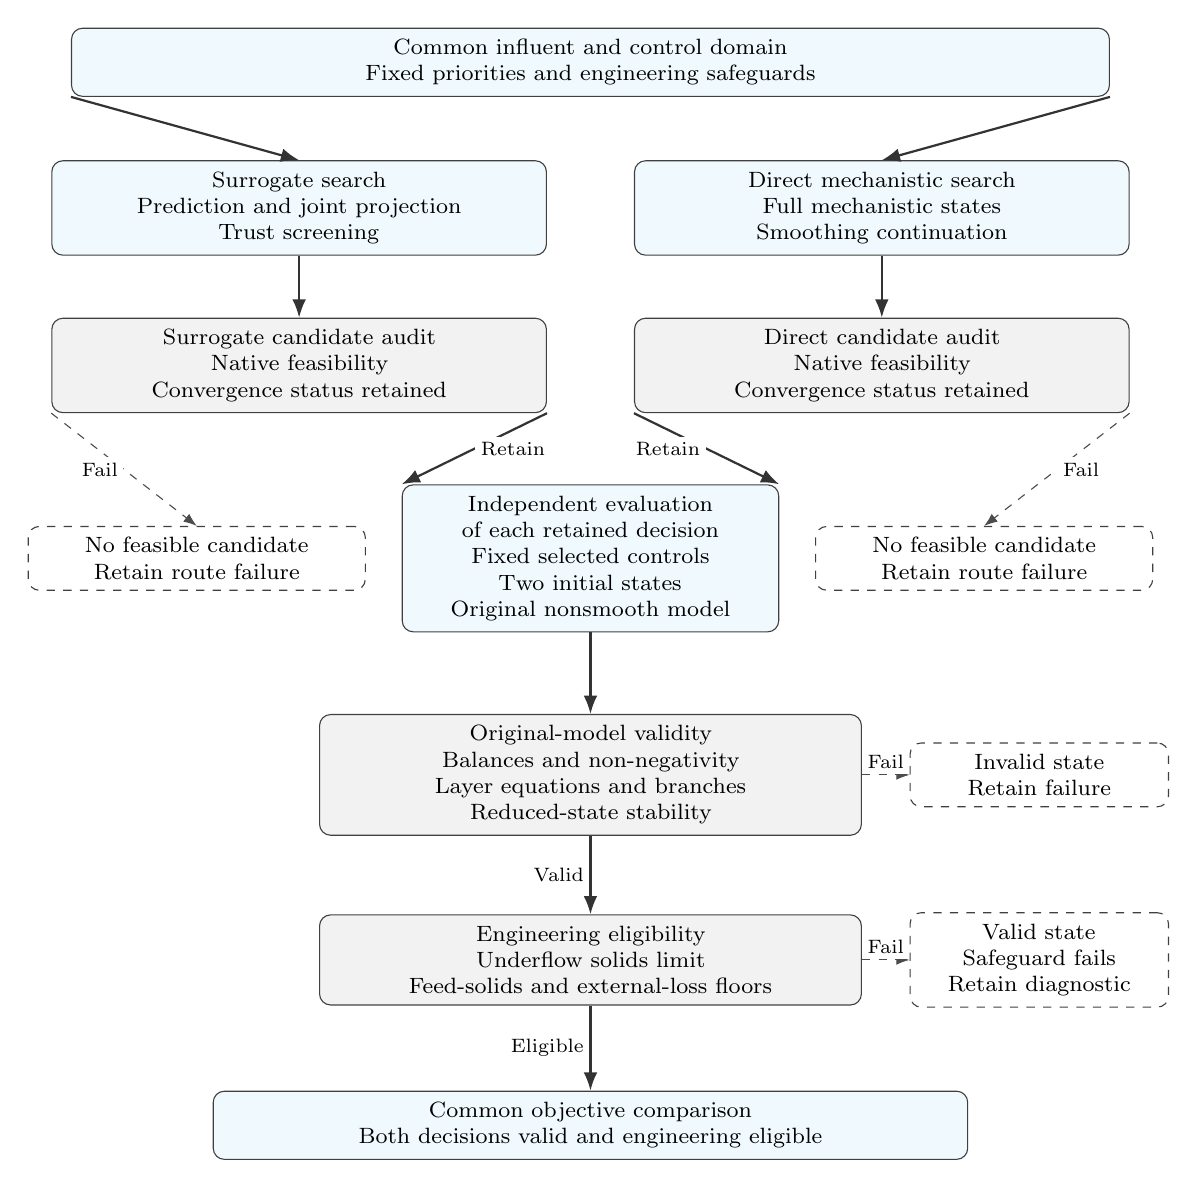
\begin{tikzpicture}[>=Latex,
block/.style={draw=black!75,rounded corners,fill=cyan!6,align=center,font=\footnotesize,inner sep=4pt},
audit/.style={block,fill=black!5},
failure/.style={block,dashed,fill=white},
flow/.style={->,thick,draw=black!80},
failflow/.style={->,dashed,draw=black!70},
lab/.style={font=\scriptsize,fill=white,inner sep=2pt}]
\node[block,text width=12.9cm] (common) at (0,0)
{Common influent and control domain\\Fixed priorities and engineering safeguards};
\node[block,text width=6.0cm] (surrogate) at (-3.7,-1.85)
{Surrogate search\\Prediction and joint projection\\Trust screening};
\node[block,text width=6.0cm] (direct) at (3.7,-1.85)
{Direct mechanistic search\\Full mechanistic states\\Smoothing continuation};
\node[audit,text width=6.0cm] (snative) at (-3.7,-3.85)
{Surrogate candidate audit\\Native feasibility\\Convergence status retained};
\node[audit,text width=6.0cm] (mnative) at (3.7,-3.85)
{Direct candidate audit\\Native feasibility\\Convergence status retained};
\node[failure,text width=4.0cm] (sfail) at (-5.0,-6.3)
{No feasible candidate\\Retain route failure};
\node[failure,text width=4.0cm] (mfail) at (5.0,-6.3)
{No feasible candidate\\Retain route failure};
\node[block,text width=4.5cm] (evaluate) at (0,-6.3)
{Independent evaluation\\of each retained decision\\Fixed selected controls\\Two initial states\\Original nonsmooth model};
\node[audit,text width=6.6cm] (valid) at (0,-9.05)
{Original-model validity\\Balances and non-negativity\\Layer equations and branches\\Reduced-state stability};
\node[failure,text width=3.0cm] (invalid) at (5.7,-9.05)
{Invalid state\\Retain failure};
\node[audit,text width=6.6cm] (engineering) at (0,-11.4)
{Engineering eligibility\\Underflow solids limit\\Feed-solids and external-loss floors};
\node[failure,text width=3.0cm] (engfail) at (5.7,-11.4)
{Valid state\\Safeguard fails\\Retain diagnostic};
\node[block,text width=9.3cm] (comparison) at (0,-13.5)
{Common objective comparison\\Both decisions valid and engineering eligible};
\draw[flow] (common.south west)--(surrogate.north);
\draw[flow] (common.south east)--(direct.north);
\draw[flow] (surrogate)--(snative);
\draw[flow] (direct)--(mnative);
\draw[flow] (snative.south east)--(evaluate.north west) node[midway,right,lab] {Retain};
\draw[flow] (mnative.south west)--(evaluate.north east) node[midway,left,lab] {Retain};
\draw[failflow] (snative.south west)--(sfail.north) node[midway,left,lab] {Fail};
\draw[failflow] (mnative.south east)--(mfail.north) node[midway,right,lab] {Fail};
\draw[flow] (evaluate)--(valid);
\draw[flow] (valid)--(engineering) node[midway,left,lab] {Valid};
\draw[failflow] (valid)--(invalid) node[midway,above,lab] {Fail};
\draw[flow] (engineering)--(comparison) node[midway,left,lab] {Eligible};
\draw[failflow] (engineering)--(engfail) node[midway,above,lab] {Fail};
\end{tikzpicture}
\caption{Conceptual paired-search and verification workflow. Each retained control vector receives its own independent original-model evaluation. The surrogate and smooth-direct native responses do not supply the reference treatment outcome. Original-model validity and engineering eligibility are distinct checks. Only eligible pairs enter the common-objective comparison, while failed or qualified cases remain in the accounting.}
\label{fig:plant_route_verification}
\end{figure}

The common evaluation stage supplies treatment responses at fixed controls rather than returning information to the fitted models. A valid physical response can still violate a retained engineering safeguard and remain useful as a diagnostic. Separating these outcomes prevents numerical convergence, physical validity, and decision eligibility from being treated as the same property.

\subsection{Evaluation at fixed selected controls}

Every available selected decision is evaluated with its controls and influent held fixed. Both initial states are solved on the original nonsmoothed reactor and ten-layer clarifier equations. This calculation does not use the statistical prediction as its treatment outcome. It also does not use the smooth direct state as proof of an exact steady state. The role of an original-model check follows the feasibility and validation requirements discussed by \citet{BhosekarIerapetritou2018}.

Exact evaluation uses the physical checks in Table~\ref{tab:plant_generation_settings}. Two-start state agreement is tested under both generation scales and fixed state scales. The fixed scales are development-set coordinatewise median absolute deviations with a floor of one. A valid evaluation must pass mass conservation, non-negativity, layer residuals, the domain, the endpoint envelope, and the reduced-state stability test.

Branch tuples must agree unless an evaluation start is boundary-ambiguous. Ambiguity bands cover the receiver threshold, zero storage capacity, zero settling offset, zero or maximum settling velocity, and equal adjacent gravitational fluxes. An ambiguity flag qualifies the state-level branch comparison. It does not prove that every mismatching branch falls within its own ambiguity band. Agreement of the physical states and all other audits is still required. Smooth stationarity or smooth-reference equivalence near such a boundary requires that qualification.

This verification is especially relevant near a prescribed nutrient limit. The aeration-scheduling framework of \citet{Ren2026} explicitly considers influent disturbances and effluent ammonium safeguards. Its safety setting is not identical to the present TN or TP objective. It reinforces the need to evaluate the particular effluent quantity and limit that governs a decision. A non-negative or mass conservation-projected concentration can still misclassify compliance.

\subsection{Native and common-reference objectives}

Let route $S$ denote the connected surrogate and route $M$ the direct smooth mechanistic search. Their native responses are $\chi_{{\rm nat},S}=\widehat\chi$ and $\chi_{{\rm nat},M}=\chi_{{\rm sm},M}$. The independently solved responses are $\chi_{{\rm ref},S}$ and $\chi_{{\rm ref},M}$. Raw and projected surrogate predictions are also evaluated, where defined, at both retained control vectors.

Route-specific normalization can change an objective even when the physical response is identical. Consider an illustrative two-quality case with positive development standard deviations 0.5 and 2 in the corresponding native units. A scale with a floor of one gives denominators 1 and 2. The unfloored scale retains 0.5 and 2. For a hypothetical response of 0.8 and 4, their standardized coordinates are
\[
\begin{aligned}
\text{floored scale}&=(0.8/1,\,4/2)=(0.8,2),\\
\text{unfloored scale}&=(0.8/0.5,\,4/2)=(1.6,2).
\end{aligned}
\]
With equal quality weights, the means are 1.4 and 1.8. This difference arises entirely from the normalization. Writing the diagonal matrices makes the componentwise denominators explicit,
\[
D_{T,S}^{\rm toy}=\begin{bmatrix}1&0\\0&2\end{bmatrix},\qquad
D_{T,M}^{\rm toy}=\begin{bmatrix}0.5&0\\0&2\end{bmatrix}.
\]
These matrices illustrate the two general definitions. The comparison of selected decisions uses one common reference normalization so that such a numerical choice is not mistaken for better treatment.

For positive development-set effluent standard deviations $\sigma_j$, native quality normalization is
\begin{equation}
D_{T,S}=\operatorname{diag}(\max(1,\sigma_j)),\qquad
D_{T,M}=\operatorname{diag}(\sigma_j).
\label{eq:plant_route_normalization}
\end{equation}
The unit floor is in the physical unit of each quality coordinate. The common reference objective uses $D_{T,M}$ for both decisions. Actual fitted standard deviations are estimation quantities and are not specified as theoretical constants.

Two distinct subtractions are needed in decision assessment. In a hypothetical surrogate route with native objective 0.90 and independent reference objective 1.10, the native-minus-reference difference is $0.90-1.10=-0.20$. This negative sign means the native calculation presents a smaller objective. It does not mean that the independently evaluated decision improves on another decision.

For an illustrative direct-route decision with native objective 0.95 and reference objective 0.98, its native-minus-reference difference is $-0.03$. Comparing the independently evaluated decisions instead gives $1.10-0.98=0.12$. On the shared objective basis, this positive difference means the surrogate-selected decision has the larger objective among these two choices. The compact expressions distinguish within-route prediction differences from between-route decision differences.

The native-to-reference and route-to-route differences are
\begin{align}
\Delta J_{{\rm nat-ref},k}&=
J_{{\rm nat},k}(\vartheta_k,\chi_{{\rm nat},k})
-J_{\rm ref}(\vartheta_k,\chi_{{\rm ref},k}),\quad k\in\{S,M\},\\
\Delta J_{S-M}&=J_{\rm ref}(\vartheta_S,\chi_{{\rm ref},S})
-J_{\rm ref}(\vartheta_M,\chi_{{\rm ref},M}).
\label{eq:plant_objective_comparison}
\end{align}
The first can reflect both response approximation and route normalization. The second compares independently evaluated decisions using a common objective basis. Neither is called regret because a global optimal objective is unavailable.

An objective comparison and a control comparison also have different denominators. A hypothetical objective difference of 0.12 with reference direct objective 0.98 has direct-relative percentage $100(0.12)/0.98\approx12.24\%$. The symmetric scaled difference uses the denominator $\max(1,1.10,0.98)=1.10$ and gives $0.12/1.10\approx0.1091$. The first uses one route as its reference. The second uses a symmetric magnitude scale with a floor.

For an illustrative control interval from 10 to 30, two selected settings of 25 and 20 differ by five physical units. Their normalized difference is $5/(30-10)=0.25$. If this is the only differing coordinate among seven, the root mean square difference is $\sqrt{0.25^2/7}\approx0.0945$, while the maximum absolute difference is 0.25. The average spreads one change over all seven coordinates. The maximum keeps the largest change visible.

Standardized response errors at each decision retain the raw, projected, and native quantities separately. A symmetric relative objective difference divides $\Delta J_{S-M}$ by $\max(1,|J_S|,|J_M|)$. A direct-relative percentage divides $100\Delta J_{S-M}$ by $J_M$ only when that denominator is nonzero. Normalized control differences are
\begin{equation}
d_j=\frac{\vartheta_{S,j}-\vartheta_{M,j}}{\vartheta_j^U-\vartheta_j^L},\qquad
d_{\rm rms}=\left(\frac17\sum_{j=1}^7d_j^2\right)^{1/2},\qquad
d_{\max}=\max_j|d_j|.
\end{equation}
These summaries distinguish similar objective values from similar controls.

Removal follows from the material entering and leaving on the stated concentration basis. For a hypothetical fresh-influent concentration of 200 mg L$^{-1}$ and an effluent concentration of 2 mg L$^{-1}$, the concentration reduction is $200-2=198$ mg L$^{-1}$. Dividing by 200 gives a fraction of 0.99, and multiplying by one hundred gives 99\%. Algebraically,
\[
100\frac{z_{{\rm in},j}-z_{E,j}}{z_{{\rm in},j}}
=100\left(1-\frac{z_{E,j}}{z_{{\rm in},j}}\right).
\]
This step requires a positive influent denominator. It compares concentrations on one reporting basis. A component inventory balance additionally uses the appropriate flow rates and represented outlets.

Selected-decision removal for composite $j$ is
\begin{equation}
\mathcal R_j=100\left(1-\frac{z_{E,j}}{z_{{\rm in},j}}\right),
\end{equation}
when the fresh-influent denominator is positive. Predicted-to-reference removal differences use percentage points. Concentration percentage errors instead divide by the mechanistic effluent concentration. For a hypothetical influent of 200 mg L$^{-1}$ and effluent values of 2 and 4 mg L$^{-1}$, the effluent prediction error is 100\% relative to 2. The removal difference is only one percentage point. Reporting both makes their different denominators clear.

\subsection{Validity, engineering eligibility, and failures}

A paired objective comparison requires both routes to supply natively feasible candidates, valid exact evaluations, and satisfaction of the common retained engineering safeguards after evaluation. A valid physical evaluation that violates an underflow, feed-solids, or external-loss safeguard still retains its diagnostic objective and treatment response. It does not enter the eligible paired comparison. Solids retention time and loading measures are reported for every finite evaluation and do not add eligibility thresholds.

\begin{table}[htbp]
\centering\small
\caption{Distinct questions retained in failure and qualification accounting.}
\label{tab:plant_failure_classes}
\begin{tabular}{p{0.31\linewidth}p{0.55\linewidth}}
\toprule Assessment & Question answered\\\midrule
Generation acceptance & Did both original-model starts pass the required physical and numerical checks?\\
Projection feasibility & Did the fitted closure and physical constraints admit an audited joint response?\\
Native engineering feasibility & Did the search candidate satisfy its declared optimization constraints?\\
Convergence qualification & Did derivative audits or complete finite polls supply their stated evidence?\\
Exact-model validity & Did independent original-model evaluation converge to an accepted state?\\
Retained engineering feasibility & Did the exact response pass the common safeguards?\\
Paired eligibility & Were both decisions available and admissible on the common reference basis?\\
\bottomrule
\end{tabular}
\end{table}

These status fields are not collapsed into one success label. Missing or nonfinite quantities, an undefined feature scale, a failed factorization, or an inconsistent numerical audit remain computational failures. A finite state that fails a scientific threshold remains a diagnostic state with the failed criterion identified. Generation rejection, optimization failure, projection infeasibility, and branch qualification have different causes and denominators.

\subsection{Influent scenarios and time accounting}

Ten influent vectors from a separate twenty-dimensional Latin hypercube define the scenario experiment. They use the seed in Table~\ref{tab:plant_design_settings} and do not enter fitting, calibration, or tuning. Both routes are attempted for the nominal influent and every scenario. Available selected decisions receive exact evaluation even when the other route fails. These cases examine sensitivity within a specified set. They do not estimate population-level reliability under arbitrary disturbances.

Optimization time is the duration of the route's initial search. For the surrogate, it includes regression, projection, and any value-only fallback inside that search. For the direct route, it includes the initial three-stage smoothing sequence. Development sampling, fitting, convergence certification, conditional recovery, and exact-model evaluation are outside this interval. Failed initial attempts remain in the time accounting. Scenario aggregates use the ten influent cases and keep the nominal case separate. Both routes use the same processor allocation and thread count.

Search time is accompanied by evaluated points, iterations, projection retries, fallback use, completed smoothing stages, recovery status, and convergence qualification. The benchmark concerns identified by \citet{Bliek2023} make these workload quantities useful when comparing expensive-function methods. Time alone cannot establish equal decision quality or equal completeness of a search.

A complete workflow account additionally includes development, certification, recovery, and verification. These costs are reported separately rather than silently absorbed into a search-speed claim. Repeated use can amortize development effort, but the relevant number of later decisions depends on the full per-decision cost and on acceptable mechanistic decision quality. A reduction in the selected search interval therefore does not by itself establish a reduction in the complete computational task.

The effect of repeated use can be shown with hypothetical total costs. Suppose development requires 100 seconds, and each later surrogate-assisted decision requires three seconds in total for search, qualification, and verification. Suppose a directly evaluated decision requires six seconds for the corresponding complete task. For twenty decisions, the costs are $100+20(3)=160$ seconds and $20(6)=120$ seconds. For fifty decisions, they are 250 and 300 seconds. These numbers illustrate amortization and are not measured computational performance.

More generally, let $n_{dec}$ be the number of later decisions, $T_{dev}$ the development cost, and $T_S$ and $T_M$ the complete per-decision costs. Expanding the comparison gives
\[
\begin{aligned}
T_{dev}+n_{dec}T_S&<n_{dec}T_M,\\
T_{dev}&<n_{dec}(T_M-T_S),\\
n_{dec}&>\frac{T_{dev}}{T_M-T_S}\qquad\text{when }T_M>T_S.
\end{aligned}
\]
The illustrative threshold is $100/(6-3)=33\tfrac13$, so at least thirty-four complete decisions are needed to cross it. If the complete per-decision cost is not smaller, a positive development cost cannot be recovered by this timing argument. The calculation also assumes that the compared decisions meet the required quality and feasibility conditions. Cost arithmetic alone does not establish that condition.

The resulting evaluation keeps four types of evidence separate. Statistical assessment concerns approximation of accepted mechanistic states. Projection audits concern the imposed network and inventory constraints. Search audits concern local numerical evidence for the declared optimization problem. Original-model verification concerns treatment and feasibility at the selected controls. This separation allows a connected surrogate to be studied as a decision aid while preserving the limits of its empirical closure and aggregate clarifier representation.

\chapter{Integrated Assessment and Research Boundaries}
\label{ch:assessment}

\section{A common basis for evaluating the prediction chain}

The research links a mechanistic component representation, statistical approximation, physical enforcement, interpretation, and operating choice. Each part introduces a specific question about credibility. The mechanistic representation defines the reference system. The statistical predictor approximates its response. The projection restricts the returned state to the imposed feasible set. Interpretation describes selected parts of the prediction map. Optimization uses the returned response to select controls. Evidence is needed at each point where the intended claim changes.

The raw benchmark and the projection benchmark share a particular prediction. This permits a paired assessment of what changes when enforcement is applied. A comparison between two independently trained models answers a different question because it also contains differences in fitting and hyperparameter selection. The structured regression adds another distinction. Its raw head, affine projection, and final constrained output are separately assessable objects. Reporting only the final output would leave the contribution of the learned structure unclear.

The connected plant adds several linked outputs. Its projection must be assessed across the mixer, reactor train, clarifier outlets, and solids inventory. A change that improves one location can worsen another while preserving joint constraints. Location-specific errors therefore remain necessary alongside a plant aggregate. This follows the general principle that approximation quality must be assessed in the quantities used by the intended decision \citep{BhosekarIerapetritou2018,McBride2019}.

\begin{table}[htbp]
\centering
\caption{Claims and the evidence required to assess them.}
\label{tab:claim_evidence}
\small
\begin{tabular}{p{0.25\textwidth}p{0.34\textwidth}p{0.31\textwidth}}
\toprule
Claim & Assessment evidence & Limit of the inference \\
\midrule
Accurate approximation & Held-out component and composite errors with defined scales & Agreement concerns the selected reference model and tested domain \\
Physical admissibility & Original equality residuals, non-negativity checks, and inventory bounds & Unimposed kinetic and dynamic relations remain unverified \\
Sample efficiency & Common learning curves and variation across partitions & The conclusion depends on the sampling and fitting budget \\
Transparent structure & Named blocks, physical-unit coefficients, and sensitivity calculations & Coefficients are predictive associations rather than identified causal laws \\
Reliable operating choice & Independent mechanistic solve at selected controls & A local search does not establish a global optimum \\
Computational benefit & Separate development, search, prediction, projection, and verification costs & Search-time savings alone do not establish a lower total cost \\
\bottomrule
\end{tabular}
\end{table}

\section{Examples that separate the assessment questions}

\subsection{Mass conservation and prediction error in the same calculation}

Consider a hypothetical two-component prediction problem in which both components use one material basis. The first reference concentration is 6 and the second is 4 in arbitrary concentration units. Their sum is $6+4=10$. The raw prediction gives 8 for the first component and 3 for the second. Its sum is $8+3=11$, so its inventory residual is $11-10=1$. Both coordinates are non-negative, but the state is inconsistent with mass conservation under the specified equality.

Suppose a hypothetical projection for mass conservation lowers the first prediction by one unit and leaves the second unchanged. The projected sum is $7+3=10$. This is one admissible projection and is not asserted to be the nearest projection under every metric. The component errors can be calculated directly,
\[
\begin{aligned}
\text{raw errors}&=(8-6,\,3-4)=(2,-1),\\
\text{projected errors}&=(7-6,\,3-4)=(1,-1),\\
\text{raw squared distance}&=2^2+(-1)^2=5,\\
\text{projected squared distance}&=1^2+(-1)^2=2.
\end{aligned}
\]
The corresponding Euclidean distances are $\sqrt5\approx2.236$ and $\sqrt2\approx1.414$. Their values follow from comparison with the reference state. The mass conservation test instead uses the predicted sums. In compact component notation, the raw state is $(8,3)^\top$, the reference state is $(6,4)^\top$, and the chosen projected state is $(7,3)^\top$. This calculation illustrates how feasibility and error are assessed on the same prediction without treating either calculation as a measured treatment outcome.

\subsection{Why the two physical requirements are simultaneous}

Now let the first hypothetical concentration be 11 and the second be $-1$. Their sum is $11+(-1)=10$, so the inventory equality is satisfied. The second component fails non-negativity. Replacing it by zero changes the sum to $11+0=11$. To return to the non-negative part of the line defined by mass conservation, both coordinates can be changed. The state with first concentration 10 and second concentration zero has sum ten and passes both checks.

The individual adjustments make the distinction explicit,
\[
\begin{aligned}
\text{raw state}&=(11,-1)^\top,\\
\text{clipped state}&=(11+0,-1+1)^\top=(11,0)^\top,\\
\text{jointly feasible state}&=(11-1,-1+1)^\top=(10,0)^\top.
\end{aligned}
\]
Clipping changes only the second coordinate. The joint projection also compensates in the first coordinate. An equality projection alone can retain a negative component, while clipping alone can violate an equality. The final assessment therefore checks both properties on the same returned state \citep{KircherVotsmeier2025,Haddad2010}.

Figure~\ref{fig:assessment_feasible_segment} places the three states on the line defined by mass conservation and its non-negative segment. Their positions show which requirement each state satisfies.

\begin{figure}[htbp]
\centering
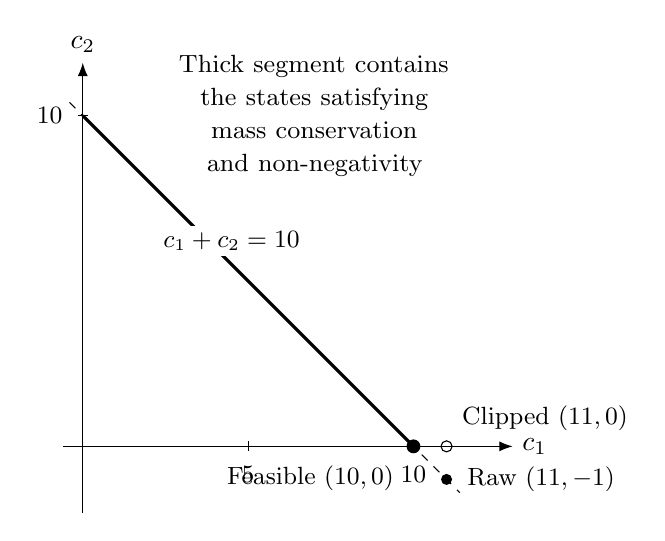
\begin{tikzpicture}[x=0.42cm,y=0.42cm,>=Latex]
\draw[->] (-0.6,0)--(13,0) node[right] {$c_1$};
\draw[->] (0,-2)--(0,11.6) node[above] {$c_2$};
\draw[dashed] (-0.4,10.4)--(11.4,-1.4);
\draw[very thick] (0,10)--(10,0);
\foreach \x in {5,10} {\draw (\x,0.15)--(\x,-0.15) node[below=2pt] {\small\x};}
\draw (0.15,10)--(-0.15,10) node[left=2pt] {\small 10};
\fill (11,-1) circle (2pt) node[right=4pt] {\small Raw $(11,-1)$};
\draw (11,0) circle (2pt) node[above right=3pt] {\small Clipped $(11,0)$};
\fill (10,0) circle (2.5pt);
\node[below left=5pt] at (10,0) {\small Feasible $(10,0)$};
\node[fill=white,inner sep=2pt] at (4.5,6.2) {\small $c_1+c_2=10$};
\node[align=center,text width=4cm] at (7,10) {\small Thick segment contains the states satisfying mass conservation and non-negativity};
\end{tikzpicture}
\caption{Hypothetical two-component geometry showing why clipping a negative concentration can violate a sum fixed by mass conservation.}
\label{fig:assessment_feasible_segment}
\end{figure}

The raw point is on the extended line defined by mass conservation but below the concentration boundary. The clipped point reaches a non-negative second coordinate while leaving that line. The jointly projected point lies at the end of the thick feasible segment. The geometry therefore makes the two simultaneous tests visible without replacing their numerical checks.

Separate marginal summaries can also be misleading. If one prediction satisfies only mass conservation and another satisfies only non-negativity, neither is jointly feasible. For a hypothetical collection of two such states, each marginal compliance frequency is one half, while the joint compliance frequency is zero. The correct denominator is the number of states checked, and both conditions are tested within each state before counting joint compliance.

\subsection{Objective comparisons at selected decisions}

A hypothetical decision comparison uses two operating choices with surrogate-predicted dimensionless objectives of $0.90$ and $0.95$. Smaller values are preferred, so prediction favors the first choice by $0.95-0.90=0.05$. Suppose independent mechanistic evaluation instead gives $1.10$ and $0.98$. On that common reference, the first choice has a larger objective by $1.10-0.98=0.12$. Relative to the second reference value, the difference is $100(0.12)/0.98\approx12.24\%$.

Both projected surrogate states could satisfy every imposed balance while this ordering changes. The value $0.12$ compares the two tested choices. It is not a gap from a known global optimum. These hypothetical arithmetic steps explain why physical consistency and average prediction error cannot establish the ordering of selected decisions \citep{Alexandrov1998,Pedrozo2025}.

\subsection{Following sensitivity through projection}

Interpretation also depends on the complete map. A positive quadratic aeration coefficient in a raw driver does not imply that every final effluent quantity increases with aeration. Coupling transforms the driver into component predictions. The reporting map combines components. The active output constraints can alter local derivatives again. Physical-unit interpretation must therefore identify whether it concerns a driver coefficient, a raw prediction derivative, or a derivative of the final projected response \citep{Brunton2016,Shen2023}.

A simplified calculation isolates the effect of projection. Let a dimensionless operating input be $a$, and let two hypothetical raw concentration equations be
\[
c_{raw,1}(a)=4+a,\qquad c_{raw,2}(a)=3+2a.
\]
The raw first-component slope is one and the second-component slope is two. At $a=2$, the concentrations are 6 and 7, with a total of 13. Suppose the required total is ten and the projection minimizes the sum of squared adjustments with equal weights. If the first adjustment is $d_1$ and the second is $d_2$, mass conservation requires $d_1+d_2=-3$. Substitute $d_2=-3-d_1$ into the squared-adjustment objective and differentiate,
\[
\begin{aligned}
d_1^2+d_2^2&=d_1^2+(-3-d_1)^2,\\
\frac{\mathrm d}{\mathrm d d_1}\bigl[d_1^2+(-3-d_1)^2\bigr]
&=4d_1+6=0.
\end{aligned}
\]
Both adjustments are $-1.5$, giving a state satisfying mass conservation with concentrations 4.5 and 5.5. For a general $a$, the excess total is $(4+a)+(3+2a)-10=3a-3$. Equal-weight projection subtracts one half of that excess from each coordinate,
\[
\begin{aligned}
c_{aff,1}(a)&=4+a-\frac{3a-3}{2}=5.5-0.5a,\\
c_{aff,2}(a)&=3+2a-\frac{3a-3}{2}=4.5+0.5a.
\end{aligned}
\]
The projected slopes are $-0.5$ and $0.5$. The first changes sign even though its raw slope is positive. The sum of the projected slopes is zero, consistent with a total that does not depend on $a$.

Non-negativity introduces another stage. The affine first component reaches zero at $a=11$. For $a>11$, the affine state lies outside the segment satisfying mass conservation and non-negativity. In this equal-weight two-component example, the nearest jointly feasible state is then $(0,10)^\top$. Both local output slopes are zero while that boundary remains active. The slope changes at the transition point. This calculation illustrates why a raw coefficient, an affine sensitivity, and a final constrained sensitivity have distinct meanings. It does not identify an aeration response of the activated sludge model.

Figure~\ref{fig:assessment_branch_sensitivity} plots the hypothetical first-component equations and the slopes calculated from them. The left panel shows the concentration returned at each stage. The right panel shows the corresponding local rate of change with respect to the operating input.

\begin{figure}[htbp]
\centering
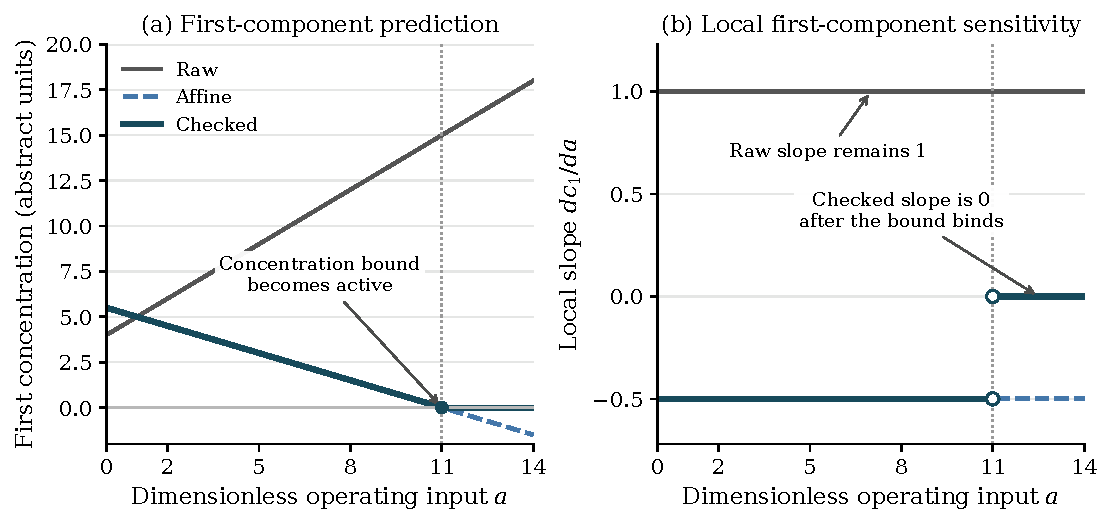
\includegraphics[width=\textwidth]{ch7_concept_branch_sensitivity.pdf}
\caption{Hypothetical first-component response and sensitivity before and after mass conservation and non-negativity enforcement. Open circles mark the two one-sided checked slopes at the active-boundary transition.}
\label{fig:assessment_branch_sensitivity}
\end{figure}

Before the boundary becomes active, the affine and checked curves coincide. Their negative first-component slope differs from the positive raw slope because mass conservation redistributes the operating response between the two components. After the boundary becomes active, the checked concentration stays at zero and its local slope is zero. The checked map has no single classical derivative at the transition itself. These visual relationships belong to the analytical illustration and do not represent fitted treatment behavior.

\section{Data separation and the status of operating evidence}

All quantities learned from data require a declared fitting reference. Input transformations, output scales, hyperparameters, regularization, overflow solids fitting, and trust calibration belong to the development information. The final assessment information is reserved for evaluating the specified procedure. This separation must remain consistent when the procedure contains a learned model followed by a constrained calculation \citep{Kaufman2012}.

The standalone reactor benchmark uses nested cross-validation to separate model selection from outer assessment. Its beyond-domain samples are simulated separately and are not used to tune the fitted predictor. The structured-regression protocol uses its declared training and holdout partitions and repeated learning-curve assessment. These designs answer related questions with different units of evidence. Their scores should not be pooled into one model ranking as if they arose from a common assessment sample.

The connected plant design distinguishes development, holdout prediction assessment, and operating verification. It also recognizes that engineering choices can be informed by earlier inspection of a simulated response. Where an analysis setting follows such inspection, mechanistic evaluation of the selected controls provides conditional evidence for that declared setting. It does not become a fully prospective assessment merely because another solve is performed. A later independent evaluation with frozen choices is needed for a stronger prospective claim \citep{Kaufman2012,Zhang2026}.

Failure accounting is part of this evidence. A failed mechanistic solve, an infeasible projection, an operating search that fails a stopping criterion, and a control that violates the original engineering constraints are different events. Omitting them changes the apparent domain and the apparent computational cost. Acceptance rules and failure counts must therefore accompany empirical assessment when it is undertaken.

\section{Limits of physical guarantees}

The reactor invariant constraints follow from the stoichiometric matrix and the compatibility of the external forcing with those invariants. They apply to the declared component representation and reactor boundary. They do not establish that every feasible concentration vector is a reachable reactor steady state. The feasible set generally contains many states that satisfy inventories and non-negativity without satisfying the nonlinear rate equations.

The plant constraints extend this logic to connected unit outputs. Mixing, flow-weighted clarifier balances, soluble-component continuity, and solids inventory bounds address specified physical relationships. Their satisfaction does not reconstruct the full layered clarifier or prove dynamic stability. The direct reference equations remain necessary for judging the selected operating controls.

Numerical feasibility also needs a declared tolerance. Exact equalities describe the mathematical formulation. Finite arithmetic and iterative solvers return approximate numerical states. A solver termination message is insufficient without residual checks in the original units or in a clearly stated scaled form. The same principle applies to the direct mechanistic comparator \citep{Boyd2004,BuzziFerraris2013}.

\section{Limits of generalization and interpretation}

Simulated training data reflect the selected process model, parameter values, and input design. A wide numerical range does not guarantee coverage of every important joint condition. A steady-state input description does not encode all dynamic or historical influences. The distinct standalone and plant alkalinity ranges also prevent an automatic transfer claim between those domains. Domain checks need to refer to the actual training representation.

Interpretation is conditional on the fitted predictor. Second-order blocks support transparent inspection, but correlated inputs and the coupling variables can produce nonunique coefficient combinations. Resampling can assess stability of structural patterns. It cannot turn a predictive coefficient into a causal biological constant. Sensitivity analysis should identify the input unit, the operating point, and the projection stage to which it applies \citep{Machado2014,Brunton2016}.

A projected point prediction also lacks an automatic uncertainty guarantee. Model ensembles, probabilistic reconciliation, and hard-constrained probabilistic learning provide other approaches to uncertainty \citep{Lakshminarayanan2017,Hansen2024,Utkarsh2025}. Their existence does not make a deterministic projection a calibrated distribution. Uncertainty remains a separate extension requiring its own assumptions and validation.

\section{Engineering interpretation of the planned assessment}

The intended assessment can identify which prediction procedures are suitable for particular uses. A rapid unconstrained approximation may be useful for exploratory analysis if its limitations are visible. A projected component state can support screening that requires declared balances and non-negativity. An interpretable constrained procedure can support inspection of named response terms. A connected plant surrogate can support an operating search when selected controls are independently checked.

The assessment must retain these different uses when interpreting empirical evidence. A smaller error does not settle every engineering requirement. A stronger physical guarantee does not settle every accuracy question. A faster search does not settle every cost question. The methodological contribution lies in making each requirement explicit and connecting it to evidence that can assess it. Treatment outcomes and empirical performance remain questions for the subsequent evaluation.


\backmatter
\bibliographystyle{apacite}
\bibliography{references}
\end{document}
